\mag 1200
%\mag 1150
%\mag 1250
%\mag 1071
\documentclass[12pt, openany, twoside]{book} % Computer Modern font calls
\usepackage[paper=a4paper, twoside, includehead]{geometry}
%\usepackage[paper=a4paper, twoside]{geometry}

\usepackage[T2A]{fontenc}
%\usepackage{literat}
%\usepackage[pdftex,unicode]{hyperref}
\usepackage[dvips]{graphicx}
\usepackage{longtable}
\usepackage[utf8]{inputenc}
\usepackage[english,russian]{babel}
\usepackage[unicode=true,colorlinks=true,pdfstartview=FitH,pdfpagemode=UseOutlines,linkcolor=black,citecolor=black,urlcolor=black,pdftitle={dis},pdfauthor={steve},pdfkeywords={},pdfproducer={LaTeX},pdfcreator={LaTeX}]{hyperref}
%\usepackage[14pt]{extsizes}
\usepackage{fancyhdr}
\usepackage{pstricks}
\usepackage{pst-all}
\usepackage{pst-poly}
\usepackage{indentfirst}
\usepackage{pscyr}
\usepackage{blindtext}
\usepackage{caption}

%\usepackage{times}
%\usepackage{pslatex}
%\def\defgeom{\geometry{paper=a5paper, left=1.4142cm, top=1.4142cm, bottom=1.4142cm,
%centering, right=1.4142cm, bindingoffset=0mm, }}
\def\defgeom{\geometry{papersize={17.5cm,24.75cm}, left=2.25cm, right=2.25cm, top=1.5cm, bottom=2.33cm, centering, bindingoffset=1mm}}
%\def\defgeom{\geometry{papersize={21cm,29.7cm}, left=2.7cm, right=2.7cm, top=1.8cm, bottom=2.8cm, centering, bindingoffset=1mm}}
%\def\defgeom{\geometry{paper=a4paper, left=2.7cm, right=2.7cm, top=1.8cm, bottom=2.8cm, centering, bindingoffset=1mm}}
%\def\defgeom{\geometry{paper=a4paper, left=2.7cm, top=1.8cm, bottom=2.8cm, -centering, right=2.7cm, bindingoffset=1mm}}
%\tolerance=10000

%Основные требования для макетов в редакторе Тех
%Поля: верхнее – 1,8 см, нижнее – 2,8, левое и правое – 2,7
%Расстояние от края страницы до колонтитула – 2,1 см

%\def\normalsize{\fontsize{15}{18}\selectfont{}}

\newenvironment{PP}{%
    \begin{quote}\tt}{%
    \end{quote}}
\def\rem#1{}


 %\renewcommand{\publishername}{Иркутский государственный технический университет}
 %\renewcommand{\locationname}{Иркутск}
%\def\AR{{\em Прим.~автора~пособия}}
 \def\baselinestretch{1}

\newtheorem{example}{Пример}[chapter]
\def\theexample{\thechapter\arabic{example}}
\newenvironment{mygroup}{}{}

 \setcounter{secnumdepth}{3}
 \setcounter{tocdepth}{3}

\defgeom{}
\makeatletter
\def\@makechapterhead#1{%
  %\vspace*{10\p@}%
  {\parindent \z@ \raggedright \normalfont
    \ifnum \c@secnumdepth >\m@ne
      \if@mainmatter
        \large\bfseries \@chapapp\space \thechapter \hbox to 0.3em {}
        %\par\nobreak
        %\vskip 5\p@
      \fi
    \fi
    \interlinepenalty\@M
    % \Large \bfseries #1\par\nobreak
    \large \bfseries #1\par\nobreak
    \vskip 7\p@
  }}
\def\@makeschapterhead#1{%
  %\vspace*{50\p@}%
  {\parindent \z@ \raggedright
    \normalfont
    \interlinepenalty\@M
    \large \bfseries  #1\par\nobreak
    \vskip 7\p@
  }}


\renewcommand\section{\@startsection {section}{1}{\z@}%
                                   {-3.25ex \@plus -1ex \@minus -.2ex}%
                                   {1.5ex \@plus.2ex}%
                                   {\normalfont\large\bfseries}}
\renewcommand\subsection{\@startsection{subsection}{2}{\z@}%
                                     {-3.25ex\@plus -1ex \@minus -.2ex}%
                                     {1.5ex \@plus .2ex}%
                                     {\normalfont\normalsize\bfseries}}
\renewcommand\subsubsection{\@startsection{subsubsection}{3}{\z@}%
                                     {-3.25ex\@plus -1ex \@minus -.2ex}%
                                     {1.5ex \@plus .2ex}%
                                     {\normalfont\normalsize\bfseries}}

\makeatother

\hypersetup{
    bookmarks=true,         % show bookmarks bar?
    unicode=true,          % non-Latin characters in Acrobat’s bookmarks
    pdftoolbar=true,        % show Acrobat’s toolbar?
    pdfmenubar=true,        % show Acrobat’s menu?
    pdffitwindow=false,     % window fit to page when opened
    pdfstartview={FitH},    % fits the width of the page to the window
    pdftitle={Dissertation 05.13.17},    % title
    pdfauthor={Alexander Larionov},     % author
    pdfsubject={Dissertation 05.13.17},   % subject of the document
    pdfcreator={LaTeX},   % creator of the document
    pdfproducer={LaTeX}, % producer of the document
    pdfkeywords={ATP} {Logics} {Artificial Intelligence}, % list of keywords
    pdfnewwindow=true,      % links in new window
    colorlinks=true,       % false: boxed links; true: colored links
    linkcolor=black, %[rgb]{0 0.4 0.1},          % color of internal links
    citecolor=black, %blue,        % color of links to bibliography
    filecolor=black,      % color of file links
    urlcolor=black % [rgb]{0.3 0.0 0.3}           % color of external links
}




\newenvironment{questions}{\subsubsection*{Вопросы для самопроверки}\begin{enumerate}}{\end{enumerate}}

%%%%%%%%%%%%%%%%%%%%%%%%%%%%%%%%%%%%%%%%%%%%%%%%%%%%
\begin{document}
\def\chaptername{}
\def\thechapter{\arabic{chapter}.}
\def\thesection{\thechapter\arabic{section}.}
\def\thesubsection{\thesection\arabic{subsection}.}
\def\thesubsubsection{\thesubsection\arabic{subsubsection}.}
\def\thefigure{\thechapter\arabic{figure}.}
\def\thetable{\thechapter\arabic{table}.}


%\fancypagestyle{plain}{%
\fancyhf{} % clear all header and footer fields
%\fancyfoot[C]{\bfseries \thepage} % except the center
\fancyhead[RE]{\small \nouppercase{\leftmark}}
\fancyhead[LO]{\small \nouppercase{\rightmark}}
\fancyhead[RO,LE]{\small \thepage}
\renewcommand{\headrulewidth}{1pt}
\renewcommand{\footrulewidth}{0pt}%}
\pagestyle{fancy}
\renewcommand{\chaptermark}[1]{\markboth{\MakeUppercase{\thechapter\ #1}}{}}
\renewcommand{\sectionmark}[1]{\markright{\MakeUppercase{\thesection\ #1}}{}}
\captionsetup[figure]{labelformat=simple,labelsep=space}
\captionsetup[table]{labelformat=simple,labelsep=newline,singlelinecheck=off,justification=raggedleft}
%\lhead{\thepage} \chead{}
%\rhead{Предисловие} \lfoot{} \cfoot{} \rfoot{}
%\renewcommand{\headrulewidth}{1pt}
\begin{titlepage}
\thispagestyle{empty}
\begin{center}{\sc
МИНИСТЕРСТВО ОБРАЗОВАНИЯ И НАУКИ \\
РОССИЙСКОЙ ФЕДЕРАЦИИ \\
ФЕДЕРАЛЬНОЕ ГОСУДАРСТВЕННОЕ БЮДЖЕТНОЕ \\
ОБРАЗОВАТЕЛЬНОЕ УЧРЕЖДЕНИЕ \\
ВЫСШЕГО ПРОФЕССИОНАЛЬНОГО ОБРАЗОВАНИЯ\\
<<ИРКУТСКИЙ ГОСУДАРСТВЕННЫЙ УНИВЕРСИТЕТ>>
    УЧРЕЖДЕНИЕ РОССИЙСКОЙ АКАДЕМИИ НАУК \\
ИНСТИТУТ ДИНАМИКИ СИСТЕМ И ТЕОРИИ УПРАВЛЕНИЯ \\
СИБИРСКОГО ОТДЕЛЕНИЯ РАН
}
\vfill
\hbox to \linewidth{\hfill Е.~А.~Черкашин\hfill}
 \vspace{2em}
{\large\bf Рекурсивно\,-\,логическое программирование}\\
{Учебное пособие}
\vfill
%\vfill
\vfill
 \textbf{Иркутск 2013}
\end{center}
\end{titlepage}

\newpage
\begin{mygroup}
\thispagestyle{empty}
\noindent УДК ---681.3.06, 004.89---

\begin{raggedright}
\hspace{6em}Печатается по решению ...
\end{raggedright}

\vfill%\footnotesize
\noindentЧ-48

{~Е.~А.~Черкашин.} {\bf Рекурсивно\,-\,логическое программирование}: Учеб.~пособие\,/~Е.~А.~Черкашин~---
Иркутск\,: Изд-во. ИГУ, 2013. --- \pageref{pg:lastpage}~c.
\vspace{1ex}
\begin{center}
\textbf{Рецензенты:} \\
к.~т.~н.~А.~Е.~Хмельнов, к.~ф.-м.~н.~А.~А.~Лемперт
\end{center}
\vspace{1ex}
Представлены лекционные материалы и лабораторные работы курса <<Рекурсивно\,-\,логическое программирование>>:базовые термины искусственного интеллекта, задачи, методы и их свойства; основы рекурсивно-логического программирования на языке Пролог; типичные задачи, решение которых лаконично представляется как рекурсивные и переборные алгоритмы. Содержит задания на лабораторный практикум по темам <<Формализация>>, <<Обработка списков>>, <<Метод Британского музея (отобразить и проверить)>> и <<Базы данных>>.

    Предназначен для студентов специальности
<<инженер-програм\-мист>>, <<инженер\,-\,системный програм\-мист>>.
Изучение материала будет полезным студентам других специальностей, так или иначе связанных с программированием, формальной логикой и комбинаторикой.

\textbf{УДК}

\textbf{ББК}

\vfill\vfill

\vfill
\hbox{}\hfill
\begin{minipage}{0.6\linewidth}
\begin{itemize}
\setlength{\itemsep}{0pt}
\setlength{\parsep}{0pt}
\item[\copyright{}] Е.~А.~Черкашин, 2013
\item[\copyright{}] ФГБОУ ВПО <<ИГУ>>, 2013
\item[\copyright{}] Институт динамики систем и теории управления СО РАН, 2013
\end{itemize}
\end{minipage}
\end{mygroup}
\tableofcontents
\clearpage

\newpage
\section*{Предисловие}
\addcontentsline{toc}{section}{Предисловие}
\thispagestyle{empty}

Предлагаемое учебное пособие разрабатывалось для студентов специальности <<инженер-программист>>, <<инженер-системный программист>>, однако может быть использовано всеми заинтересованными программистами, желающими овладеть некоторыми методами искусственного интеллекта. Пособие включает в себя рефе\-ра\-тив\-ную подборку материала по курсу <<Рекурсивно-логическое программирование>>, а также варианты лабораторных работ и методические указания по их выполнению. Оно никоим образом не претендует на полноту излагаемого материала и базируется на личном опыте преподавания.

Пособие можно воспринимать как путеводитель, и учащиеся в процессе обучения должны активно использовать литературу, на которую в тексте указаны ссылки. Если в конце первого предложения первого абзаца раздела стоит ссылка, например, <<\cite{AIDictionary}>>, то в основу этого раздела лег материал из указанного источника. Автор пособия корректировал некоторые неточности\footnote{\ldots и вносил свои ;-).}, адаптировал текст и примеры к нуждам преподаваемого курса и к свойствам используемого программного обеспечения. В цитируемом тексте в виде сносок автор позволяет себе высказывать то или иное отношение к изложенному.

В тексте пособия использована следующая разметка:
\begin{description}
\item[Жирным шрифтом] выделяются имена существительные и глаголы, на которые, по мнению автора, следует обратить внимание, это --- что-то вроде дополнительной семантической разметки текста учебного пособия.
\item[\normalfont{\tt Шрифтом печатной машинки (Courier)}] приводятся программы, отрывки программ в основном тексте пособия, а также имена идентификаторов, т.~е. все, что имеет отношение к {\bf тексту программы}.
\item[\normalfont{\em Наклонным шрифтом (italic)}] выделяются {\bf новые}, вводимые в текст термины, возникающие, например, в определениях, а также текст выделенных примеров.
\item[\normalfont С помощью <<кавычек>>] выделяются метафоры, значения, новые знаки текстов программ, цитаты, слова, использованные в переносном смысле, и т.~д.
\item[\normalfont{\sf Рубленым шрифтом (sans serif) или {\sl наклонным (slated)}}] декориру\-ют\-ся тексты, которые просто надо как-то выделить на общем фоне.
\end{description}

Надеюсь, что изучение такого интересного раздела информатики как <<Искусственный интеллект>>, к которому относится рекурсивно-логическое программирование, доставит учащимся не меньше удовольствия, чем в свое время автору этого учебного пособия.

Автор признателен академику Российской академии наук С.~Н.~Васильеву за создание плодотворной почвы для проведения научных исследований в области систем искусственного интеллекта. Автор благодарит преподавателей Института кибернетики, Кафедры вычислительной техники Национального исследовательского Иркутского государственного технического университета, а также преподавателей Института математики, экономики и информатики Иркутского государственного университета за предоставление возможности изучать область искусственного интеллекта.

Автор благодарит канд.~геол.-минерал.~наук Т.~Ю.~Черкашину, канд.~техн.~наук  А.~К.~Попову за помощь в подготовке данного учебного пособия.

\medskip
\noindent\hbox to \linewidth{\hfill\sf С.~н.~с. ИДСТУ СО РАН, доцент кафедр ВТ ИрГТУ и ИТ ИМЭИ ИГУ}
\noindent\hbox to \linewidth{\hfill\sf канд.~техн.~наук Е.~А.~Черкашин}
%\noindent\hbox to \linewidth{\hfill\sf аспирант кафедры ИТ ИМЭИ ИГУ}
%\noindent\hbox to \linewidth{\hfill\sf И.~Н.~Терехин}

\vfill
\makeatletter
\noindent{\sf P.~S.} Автора всегда можно найти по адресу \href{mailto:eugeneai@icc.ru}{eugeneai@icc.ru}, в поле <<{\tt тема}>> прошу указывать <<РЛП-2013>>.
\makeatother

\chapter{Введение в область искусственного интеллекта}

Среди задач, которые решают современные программисты, выделяются задачи создания программных систем математического моделирования и прогнозирования, проектирования и реализации информационных систем (ИС) и баз данных (БД), системного программного обеспечения (СПО). Все перечисленные задачи объединяет одно общее свойство --- для широкого практического класса задач можно построить детерминированную процедуру (например, алгоритм) их решения. Существует большой класс задач, для которых такую процедуру построить достаточно сложно, а порой и невозможно. Например, разработать игровую систему, способную играть в шахматы с человеком на достаточно высоком профессиональном уровне. К таким задачам относятся также и задачи поиска решения (планирование действий, или Problem Sol\-ving), распознавание образов, экспертные консультации, интеллектуальное управление сложными динамическими объектами и т.~д. В каждой такой задаче четко вырисовывается их первое общее {\bf свойство} --- необходимость {\bf автоматизации принятия некоторого решения}. В других задачах четко вырисовывается еще одно свойство --- {\bf обработка символьной информации}. Примерами задач, обработка информации в которых основывается на преобразовании строк символов, выступают следующие задачи: автоматический перевод текста с одного естественного языка на другой, автоматическое доказательство теорем. В той или иной мере оба выделенных свойства присутствуют в каждой из перечисленных задач.

Рекурсивно-логическое программирование позволяет представить решение таких задач, алгоритм, в рекурсивном виде или в виде некоторого переборного процесса. Такое представление обладает одним полезным свойством --- оно компактно и достаточно близко к исходной математической модели задачи по сравнению с изученной ранее процедурной парадигмой программирования. Программисту не требуется определять все действия, необходимые для достижения результата. Как правило, достаточно рассказать транслятору, какие данные есть в наличии, объяснить, как они связаны друг с другом и постановкой задачи. Система постарается получить решение самостоятельно. Рекурсивно-логическое программирование прежде всего направлено на решение задач искусственного интеллекта (ИИ)\footnote{В англоязычной литературе данный термин называется \emph{Artifical Inelligence, AI}. }, поэтому в данном учебном пособии необходимо ввести читателя в базовые концепции ИИ. Для начала рассмотрим, как можно определить, относится ли ваша задача к задачам ИИ.

Рассмотрим задачи планирования действий (Problem Sol\-ving). Что есть решение в этих задачах? Это --- ответ на вопрос <<Какие действия необходимо выполнить и в каком порядке их надо выполнять, чтобы достичь цели из некоторого начального состояния?>>. Получается, что ответ на этот вопрос есть некоторая конечная последовательность действий. Эта последовательность представляется в памяти компьютера в виде некоторого ряда чисел, кодирующего эту последовательность. Построить (найти) эту последовательность, выбрать последовательность из возможных альтернатив --- это и есть принятие решения.

Есть еще один интересный аспект алгоритма --- массовость, т.~е. алгоритмы должны строиться для некоторого класса задач, а не для конкретных входных данных. Что это значит? На вход программы, реализующей алгоритм, подаются какие-либо входные данные, задающие конкретную задачу из класса решаемых алгоритмом задач. Теперь представим такую ситуацию, что на вход алгоритма невозможно подать все необходимые данные, т.~е. имеет место \emph{неполнота информации}. Или другой вариант --- имеется два разных набора данных, относящихся к одной и той же задаче. Какие данные следует передавать на вход алгоритма? Этот случай связан с \emph{противоречивой информацией}. Разрабатывая программное обеспечение, позволяющее функционировать в таких условиях, приходится создавать подпрограммы, принимающие решение, что следует делать. Например, во втором случае можно запустить алгоритм для каждого набора данных и проанализировать полученные результаты. Может получиться так, что эти результаты не будут сильно отличаться друг от друга.

Задачи,  обладающие перечисленными свойствами, и методы их решения на ЭВМ в конечном счете составляют предмет исследования искусственного интеллекта --- одного из разделов информатики (Computer Science).

\section{Термин <<искусственный интеллект>>}

В литературе можно найти целый спектр определений термина искусственный интеллект, однако, насколько известно автору, ни один из них не принят как стандарт.

Среди многих точек зрения доминируют три \cite{AIDictionary}. Согласно {\bf первой}, исследования в области искусственного интеллекта являются фундаментальными исследованиями, в рамках которых разрабатываются модели и методы решения задач, традиционно считавшихся интеллектуальными и не поддававшихся ранее формализации и автоматизации. Согласно {\bf второй} точке зрения, новое направление связано с новыми идеями решения задач на ЭВМ, с разработкой принципиально иной технологии программирования, с переходом к архитектуре ЭВМ, отвергающей классическую архитектуру, которая восходит еще к первым ЭВМ. Наконец, {\bf третья точка зрения}, по-видимому, наиболее прагматическая, состоит в том, что в результате работ в области искусственного интеллекта рождается множество прикладных систем, решающих задачи, для которых ранее создаваемые системы были непригодны.

Достаточно простые определения {\em искусственного интеллекта} показаны в табл.~\ref{pic:determai} \cite{Russell}. Выделяются несколько комбинаций двух пар ключевых терминов: <<размышлять>> и <<вести себя>>, <<как человек>> и <<рационально>>.

\begin{table}[h]
\caption{Несколько определений искусственного интеллекта} \label{pic:determai}
\begin{center}
\begin{tabular}{|p{0.4\linewidth}|p{0.4\linewidth}|}
 \hline
 \begin{raggedright}
   Системы, которые размышляют, как люди.
 \end{raggedright}
 &
 \begin{raggedright}
   Системы, которые размышляют рационально.
 \end{raggedright}
 \\\hline
 \begin{raggedright}
   Системы, которые ведут себя, как
   люди.
 \end{raggedright}
 &
 \begin{raggedright}
   Системы, которые ведут себя рационально.
 \end{raggedright}
   \\\hline
\end{tabular}
\end{center}
\end{table}

{\em Искусственный интеллект} как наука насчитывает уже около 60 лет. Задачей этой науки является воссоздание с помощью искусственных устройств (в основном с помощью ЭВМ) разумных рассуждений и действий \cite{Lauriere}.\\
{\em Искусственный интеллект} --- раздел информатики, изучающий методы, способы и приемы моделирования и воспроизведения с помощью ЭВМ разумной деятельности человека, связанной с решением задач \cite{math_slov:88}.

\subsection{Тест Тьюринга}

В книге \cite{Russell} вводится понятие {\em агента}. {\em Агент} --- субъект, находящийся в среде, имеющий цель своего существования, взаимодействующий со средой или другими агентами с помощью {\em рецепторов} и {\em эффекторов}. Рецепторы воспринимают информацию о среде, а эффекторы --- это способ воздействия на среду, которое меняет среду, а следовательно, и информацию о среде. Агентом может являться как программа, так и человек. Вводится понятие {\em интеллектуального агента} --- агента, обладающего интеллектом.

Агенты взаимодействуют друг с другом. Примером такого взаимодействия выступают, например, общение человека с человеком или работа человека с компьютерной программой.

Тест Тьюринга предложен Аланом Тьюрингом (1950), и был разработан, чтобы <<обеспечить>> действующее определение интеллекта \cite{Russell}. Тьюринг определял интеллектное поведение как <<возможность>> достижения человеческого уровня производительности во всех задачах, где возможно обмануть <<вопрошающего>>. Грубо говоря, предложенный им тест состоял в следующем. Компьютеру задает вопросы человек через удаленное устройство. Тест считается пройденным, если человек не может сказать, кто или что на другом конце устройства: компьютер или человек.

С точки зрения агентов, этот тест можно представить так: один интеллектуальный агент (человек) по информационному каналу, не позволяющему ему использовать иную информацию, кроме ответов на поставленные им вопросы, анализирует поступающую информацию (ответы собеседника) от другого агента (испытуемого). Если первый агент не в силах определить, кто на другом конце информационного канала --- человек или устройство, тогда считается, что испытуемый агент обладает интеллектуальными свойствами.

\subsection{Применение искусственного интеллекта}

Всякая задача, для которой неизвестен алгоритм решения, априорно относится к ИИ. Перечислим некоторые задачи ИИ:
\begin{description}
 \item [Восприятие и распознавание образов.] К таким задачам относятся распознавание текста (как печатного, так и рукописного), компьютерное зрение.
 \item [Автоматическое доказательство теорем.] По крайней мере, следующие две задачи включены в эту область ис\-сле\-до\-ваний: автоматизация математических исследований, разработка формальных (математических) методов логического вывода для поддержки решения других задач ИИ. Это направление нашло применение в задачах верификации программного и аппаратного обеспечения.
 \item [Игры.] Автоматизация решения игровых задач, например, игры в шахматы, кал\'{а}х, реверси, а также других игр.
 \item [Решение задач (Problem Solving), планирование.] В этих задачах предполагается наличие некоторого выбора из возможных путей решения, требуется найти первое, лучшее или оптимальное решение. Примеры: составление расписания работы учебного учреждения, планирование действий робота.
 \item [Понимание естественного языка.] Как правило, си\-сте\-мы понимания естественного языка являются составляющими информационных систем различного назначения: от автоматических систем заказа билетов до систем ввода экспертного знания.
 \item [Логические языки программирования.] Языки программирования  высокого выразительного уровня, построенные на основе результатов исследования формально-ло\-ги\-чес\-ких систем, теорий исчислений. Эта область ИИ носит, кроме прочего, инструментальный характер, т.~е. с помощью средств логического программирования реализовано много систем ИИ.
 \item [Экспертные системы.] Экспертные системы  (ЭС) позволяют заменять человека-эксперта в некоторой предметной области программной системой, способной проводить экспертные консультации пользователя. ЭС нашли широкое применение в индустрии.
 \item [Интеллектные информационные системы.] Такие сис\-те\-мы представляют собой совокупности  разнородных интеллектных систем (например, системы речевого общения, решения задач и др.) для организации интеллектного доступа, обработки информации. Они, как правило, предназначены для работы с конечным пользователем низкой квалификации. Пример: электронные переводчики и разговорники.
 \item [Восприятие и усвоение знаний.] Одна из задач ИИ --- это приобретение знаний\footnote{\emph{Англ.} --- Knowledge Acquisition.} (обучение, наполнение базы знаний) от человека или самостоятельно из среды функционирования. Системы усвоения знаний используются как подсистемы других интеллектных систем.
 \item [Интеллектное управление \cite{Vass:2000}.] Новое направление, появившееся на стыке ИИ и теории управления, в котором разрабатываются управляющие системы, основанные на тех или иных методах ИИ. В настоящее время наиболее развиты методы управления на основе нечеткой логики и искусственных нейронных сетей. В этом новом направлении ведутся научные разработки Института динамики систем и теории управления СО РАН (\url{http://www.idstu.irk.ru}) (г.\,Иркутск).
\item [Робототехника (Robotics).] Тоже собирательное направление, призванное авто\-ма\-ти\-зировать работу роботов, вплоть до полной независимости их от человека.
\end{description}

\subsection{Определение задач ИИ в контексте пособия}

К сфере искусственного интеллекта относятся задачи, обладающие следующими свойствами \cite{Lauriere}:
 \begin{itemize}
 \item в них используется информация в символьной форме: буквы, слова, знаки, рисунки. Это отличает область ИИ от областей, в которых традиционно компьютерам доверяется обработка данных в числовой форме\footnote{Например, математическое моделирование, базы данных.};
  \item в них предполагается наличие выбора; действительно, сказать, что не существует алгоритма\footnote{Интуитивное определение алгоритма: \emph{алгоритм} --- это конечная последовательность действий, каждое из которых выполняется за конечное время, приводящая к определенному результату.}, --- это значит сказать, по сути дела, только то, что нужно сделать выбор между многими вариантами в условиях неопределенности, и этот недетерминизм, который носит фундаментальный характер, эта свобода действия являются существенной составляющей интеллекта.
 \end{itemize}

Излагаемый в пособии курс подразумевает непосредственное изучение технических аспектов применения методов ИИ, таких как применимость того или иного метода в конкретной задаче, реализация программных модулей конкретного метода. Поэтому в предлагаемом курсе мы будем использовать следующее определение искусственного интеллекта:
\begin{quote}{\em
Искусственный интеллект} --- область информатики, в которой разрабатываются и исследуются методы построения программных систем и решения задач так или иначе связанных с принятием решения и обработкой символьной информации\footnote{Данное определение задает термин в достаточно узком смысле.}.
\end{quote}

\section{Данные и знания}

Одним из фундаментальных терминов ИИ является термин {\em знание}. Данный термин также является сложным в смысле его конструктивного определения, понятного читателю. Как правило, авторы статей по ИИ сознательно уклоняются давать более или менее точные определения, предполагая, что читателю это уже известно.

Более формальный термин <<данные>> получил широкое распространение в научно-техническом обиходе, в особенности в практике использования ЭВМ для решения самых разнообразных задач \cite{AIDictionary}. При этом вся обрабатываемая информация называется данными: началь\-ны\-ми, промежуточными или конечными, входными или выходными. Для предложений естественного языка более привычен термин <<знание>>, а чаще --- связанный с ним глагол <<знать>>. Ни у кого не вызывает возражений использование этого слова в предложениях вроде <<я знаю, как решить задачу>>, или <<я знаю, что вчера Петя встречался с Наташей>>. Сомнению может подвергаться лишь истинность подобных утверждений, но никак не возможность сочетания слова <<знать>> с фрагментами предложения, обозначающих любую информацию, о которой говорится, что она кому-то известна.

Вопрос о разделении информации на данные и знания возник при разработке систем ИИ, определяемых в последнее время как системы, основанные на знаниях\footnote{На самом деле это определение не охватывает такую важную отрасль ИИ, как нейронные сети.}. Был предложен ряд определений, отражающих различные аспекты этих понятий, но касающихся скорее форм (см. раздел \ref{sec:knowlege_repr} представления данных и знаний, правил их использования, чем их сути.

\paragraph{Два подхода к разработке методов и средств ИИ}
\begin{mygroup}
\small\sf
\begin{description}
\item[<<Снизу-вверх>>.] Суть подхода выражена в фразе <<{\em Давайте создадим механическое (вычислительное) устройство, похожее на (моделирующее) мозг человека, а затем посмотрим как, оно будет решать задачи ИИ}>>.
\item[<<Сверху-вниз>>.] В основе этого подхода лежит {\em разработка методов моделирования процесса мышления человека (логических выводов, логических рассуждений}.
\end{description}

Методы и системы ИИ, основанные на подходе <<Снизу-вверх>>, как правило, представляют собой сложную сеть взаимосвязанных, простых по сути, элементарных агентов. Эта сеть агентов формирует агента высокого уровня, направленного на решение конкретной задачи ИИ. Элементарные агенты сети вносят небольшой персональный вклад в решение агента высокого уровня. Выделяют одно из достоинств этого подхода --- {\em если задача <<не решается>> какими-то формальными методами, то ее <<хоть какое-то>> решение может быть получено методами <<Снизу-вверх>>}. Как правило, схема применения описываемых методов и систем состоит из двух этапов: {\bf обучение} на известном наборе <<данные --- решения>> (данные и решения известны) и {\bf решения} новых задач (данные известны, решения --- нет).

Недостатком, присущим методам и системам <<Снизу-вверх>>, является неопределенность характеристик с точки зрения их практического применения: трудно ответить, например, на вопросы: <<Сколько нужно агентов, чтобы решить конкретную задачу? Каковы должны быть связи между агентами?>>. В каждом конкретном случае требуются эмпирические исследования (<<сможет\,{}-\,{}не сможет>>).

Типичным представителем подхода <<Снизу-вверх>> являются нейронные сети.

Моделирование логических выводов и рассуждений --- основа подхода <<Сверху-вниз>>. В системах ИИ (агентах), основывающихся на этом подходе, как правило, {\bf четко выделяют} функциональные блоки <<Хранилище Базы знаний>>, <<Машина логического вывода>> и <<Интерфейс Ре\-цеп\-тор\,{}-\,{}Блок рас\-суж\-де\-ний\,{}-\,{}Эффек\-тор>>. В задачу последнего блока входит преобразование информации в/из вид(а), используемый(ого) в первых двух блоках. Именно в этих методах и системах ИИ возникает задача представления знаний в некотором формализованном виде, удобном для осуществления их интерпретации и преобразований в блоке <<Машина логического вывода>>. Примерами\rem{\footnote{Мы не будем анализировать здесь достоинства и недостатки этих методов, т.~к. все это будет изложено в пособии.}} систем <<Сверху-вниз>> выступают язык программирования Пролог, экспертные системы, системы автоматического логического вывода.

\end{mygroup}

Исходя из общих соображений, естественно определить данные как некоторые сведения об отдельных объектах, а знания --- о мире в целом. В согласии с таким подходом будем считать, что:
\begin{quote}
{\em Данные} представляют информацию о существовании объектов с определенными комбинациями свойств\linebreak{} (значений признаков), а {\em знания} --- информацию о существующих в мире закономерных связях между признаками, запрещающих некоторые другие сочетания свойств у объектов.
\end{quote}

Отсюда следует, что различие между данными и знаниями можно сфор\-му\-ли\-ро\-вать так: {\em данные} --- это информация о существовании объектов с некоторым набором свойств, а {\em знания} --- информация о несуществовании объектов с некоторым набором свойств\footnote{С научной точки зрения данное предложение не является определением, оно неконструктивно, т.~е. не задает логических связей с известными объектами и терминами. В частности, термин <<навык>> тоже подходит под это же определение.}.

Используя логический формализм (см. далее) представления знаний, продемонстрируем эти понятия в формализованном виде. Отображая наличие упомянутых наборов предикатами $P$ и $Q$, можно представлять {\em данные} утверждениями с кванторами существования
$\exists$:
$$
    \exists w: P(w),
$$
а {\em знания} --- утверждениями с его отрицанием $\neg\exists$:
$$
    \neg\exists w: Q(w),
$$
легко преобразуемыми в утверждения с квантором всеобщности
$\forall$:
$$
    \forall w: \neg Q(w).
$$
Вообще говоря, последняя форма (с использованием отрицания некоторого высказывания) практически не используется. Однако используется форма, подобная этой --- $\forall w: A(w)\to B(w)$. Здесь, по сути, важен факт присутствия квантора всеобщности, говорящего, что {\bf все объекты} $w$, обладающие свойством $A$, будут обладать свойством $B$.

Тремя базовыми элементами как практической, так и теоретической рациональной деятельности являются\footnote{Одно из последних, найденных автором пособия в \cite{DDWII}, определений.} следующие \cite{DDWII}:

    {\em Данные}, которые должны прежде всего храниться, а затем, в порядке убывания приоритетов для непосредственной применимости, успешно находиться при нужде, проверяться, поддерживаться в порядке и обновляться при необходимости. Таким образом, они хранятся неизменными, пока не будут явно обновлены, и поэтому обычно внимание уделяют прежде всего сохранению, поддержанию их адекватности меняющемуся состоянию дел и целостности при необходимых изменениях.

    {\em Знания} должны прежде всего преобразовываться. Далее, их нужно хранить, как и данные, они должны быть доступными, они должны конкретизироваться применительно к данной ситуации и обобщаться для целого класса применений. Они, конечно же, должны при необходимости пересматриваться. И, наконец, они должны переводиться с одного языка на другой.

    {\em Умения} прежде всего применяются. Помимо этого, они преобразуются для обеспечения гибкости или приспособления к изменившимся условиям. Далее, они обобщаются и пересматриваются.\\[1ex]

При исследовании естественных предметных областей данные представляют первичную информацию, получаемую путем обнаружения некоторых объектов и выявления их свойств --- измерения значений признаков. Знания --- результат переработки данных, их обобщения. Классическим примером данных служат таблицы движения планет по небесному своду Тихо Браге, примером знаний --- выведенные из них законы Иоганна Кеплера и, затем как обобщение результатов Кеплера, закон всемирного тяготения Исаака Ньютона.

\section{Формализмы представления знаний}
\label{sec:knowlege_repr}


В интеллектуальных системах (ИС) используются различные способы представления знаний. Наиболее известные из них --- это {\em логический}, {\em сетевой}, {\em продукционный} и {\em фреймовый} формализмы\footnote{Некоторый формальный способ записи чего-либо.} (модели) представления знаний.

\subsection{Логические модели}

 В основе такого типа лежит формальная система, задаваемая четверкой типа $M=\langle T, P, A, B\rangle$ \cite{AIDictionary}. Множество $T$ есть множество базовых элементов различной природы, например, слов из некоторого ограниченного словаря, деталей детского конструктора, входящих в состав некоторого набора, и т.~п. Важно, что для множества $T$ существует некоторый способ определения принадлежности или непринадлежности произвольного элемента к этому множеству. Процедура такой проверки может быть любой, но за конечное число шагов она должна давать положительный или отрицательный ответ на вопрос, является ли $x$ элементом множества $T$. Обозначим эту процедуру $\Pi(T)$.

Множество $P$ есть множество синтаксических правил. С их помощью из элементов $T$ образуют синтаксически правильные совокупности. Например, из слов ограниченного словаря строятся синтаксически правильные фразы, из деталей детского конструктора с помощью гаек и болтов собираются новые конструкции. Декларируется существование процедуры $\Pi(P)$, с помощью которой за конечное число шагов можно получить ответ на вопрос, является ли совокупность $x$ синтаксически правильной.

Во множестве синтаксически правильных совокупностей выделяется некоторое подмножество $A$. Элементы $A$ называются аксиомами. Как и для других составляющих формальной системы, должна существовать процедура $\Pi(A)$, с помощью которой для любой синтаксически правильной совокупности можно получить ответ на вопрос о принадлежности ее к множеству $A$. Множество $B$ есть множество правил вывода. Применяя их к элементам $A$, можно получать новые синтаксически правильные совокупности, к которым снова можно применять правила из $B$. Так формируется множество выводимых в данной формальной системе совокупностей. Если имеется процедура $\Pi(B)$, с помощью которой можно определить для любой синтаксически правильной совокупности, является ли она выводимой, то соответствующая формальная система является разрешимой. Это показывает, что именно правила вывода являются наиболее сложной составляющей формальной системы.

Для знаний, входящих в базу знаний, можно считать, что множество $A$ образует все информационные единицы, которые введены в базу знаний (БЗ) извне, а с помощью правил вывода из них выводятся новые производные знания. Другими словами, {\em формальная система} представляет собой {\bf генератор порождения новых знаний}, образующих множество выводимых в данной системе знаний $D$. Это свойство логических моделей делает их притягательными для использования в базах знаний. Оно позволяет хранить в базе лишь те знания, которые образуют множество $A$, а все остальные знания из $D$ получать из них по правилам вывода.

\begin{example} Здесь и далее рассмотрим, как можно представить следующий набор высказываний (данных и знаний)\footnote{В разделе рассматривается только представление знаний. Тот факт, что Сократ смертен, нас не интересует\ldots пока.}:
\label{ex:repr:main}
\begin{enumerate}
\item Все люди смертны.
\item Сократ --- человек.
\end{enumerate}
\end{example}

Для начала введем наш язык (элементы детского конструктора). Пусть $H(x)$ обозначает фразу <<$x$ является человеком>>, а $M(x)$ --- <<$x$ --- смертен>>. Необходимо заметить, что $x$ как элемент языка представляет объекты предметной области, которыми в нашем случае выступают люди\footnote{\ldots Может быть и животные, однако это нас не интересует, так как знания связывают только свойства $H$ и $M$.}. Можно выделить и отдельные объекты, например Сократа --- <<$s$>>. Теперь позаимствуем еще несколько символов из исчисления предикатов первого порядка, а именно, $\forall$, $\to$, скобки и др. Теперь первое высказывание представляется как
$$
\forall x \left(H(x)\to M(x)\right).
$$
Это высказывание является {\em знанием}. Второе высказывание ---
$$
H(s).
$$
Это --- \emph{данные}, т.~е. существует Сократ, который смертен.

\subsection{Сетевые модели}

В основе моделей этого типа лежит конструкция, названная ранее семантической сетью. Сетевые модели формально можно записать в виде
$$
    H=\langle I, C_1, C_2, \ldots, C_n, \Gamma\rangle.
$$
Здесь $I$ есть множество информационных единиц; $C_1, C_2, \ldots, C_n$ --- множество типов связей между информационными единицами. Отображение $\Gamma$ задает между информационными единицами, входящими в $I$, связи из заданного набора типов связей. В зависимости от типов связей, используемых в модели, различают {\em классифицирующие} сети, {\em функциональные} сети и {\em сценарии}.

В {\bf классифицирующих} сетях используются различные отношения структуризации. Такие сети позволяют в базу знаний вводить различные иерархические отношения между информационными единицами. {\bf Функциональные} сети характеризуются наличием функциональных отношений. Их часто называют вычислительными моделями, так как они позволяют описывать процедуры вычислений одних информационных единиц через другие. В \textbf{сценариях} используются казуальные\footnote{Скорей всего, это слово образовано от англ. <<case>>, что значит <<случай>>. Здесь имеется в виду различение некоторых типовых ситуаций и осуществление некоторого действия в этой ситуации.} отношения, а также отношения типов <<средство~---~результат>>, <<орудие~---~действие>> и т.~п.

Если в сетевой модели допускаются связи различного типа, то ее обычно называют {\em семантической} сетью. Примером семантической сети представления знаний является энциклопедический словарь. Такой словарь содержит определения одних понятий через другие. Как правило, в определениях выделяются те базовые определения, которые содержатся в этом словаре.

На рис.~\ref{pic:repr:semnet} представлен пример \ref{ex:repr:main} в виде семантической сети. В вершинах графа располагаются термины и объекты: <<Человек>>, <<Смертный>>, <<Сократ>>. Дуги графа --- это логические связи между терминами и объектами: <<являться>> (в англоязычной литературе это отношение принято называть <<is\_a>>).
\begin{figure}\small
\begin{center}%
  %\psset{linewidth=1pt, linecolor=black}
  %\setlength{\arraycolsep}{5em}
  %\def\arrayrowsep{7ex}
  \begin{tabular}{cc}
	\rnode{s}{\psframebox{Сократ}}\hbox to 5em {} &
    \psframebox[linecolor=white, linestyle=none]{
    \begin{tabular}{cc}
      \rnode{h}{\psframebox{Человек}}\hbox to 5em{} &
      \rnode{m}{\psframebox{Смертный}}
    \end{tabular}
    }
  \end{tabular}
\psset{nodesep=0pt,arrows=->}%
%\ncline[linestyle=dotted]{s}{h}\naput{{\small является}}
\ncline{s}{h}\naput{{\small является}}
\ncline{h}{m}\naput{{\small является \vbox to 5em{}}}%
\end{center}%
\caption{Пример представления данных и знаний в виде семантической сети}
\label{pic:repr:semnet}
\end{figure}

\subsection{Продукционные модели}

В моделях этого типа используются некоторые элементы логических и сетевых моделей. Из логических моделей заимствована {\bf идея правил вывода}, которые здесь называются {\em продукциями}, а из сетевых моделей --- описание знаний в виде семантической сети \cite{AIDictionary}.

В результате применения правил вывода к фрагментам сетевого описания происходит трансформация семантической сети за счет смены ее фрагментов, наращивания сети и исключения из нее ненужных фрагментов. Таким образом, в продукционных моделях процедурная информация явно выделена и описывается иными средствами, чем декларативная информация. Вместо логического вывода, характерного для логических моделей, в продукционных моделях появляется вывод на знаниях.

Рассмотрим продукционное представление примера \ref{ex:repr:main}. В виде сети представим второе высказывание --- <<Сократ --- человек>>, а первое высказывание представим в виде правила преобразования участка сети в другой вид. Правила преобразования можно представлять в виде структур <<Если \ldots, то \ldots >>, т.~е., в нашем случае: <<Если $x$ --- человек, то $x$ --- смертен>>. Полученное представление данных и знаний изображено на рис. \ref{pic:repr:prod}.

\begin{figure}\small
\begin{center}
\begin{tabular}{c|c}
Данные & Знания
\\
\hline
&
\\
  \begin{tabular}{cc}
	\rnode{s}{\psframebox{Сократ}}\hbox to 3em {} &
    \rnode{h}{\psframebox{Человек}}
  \end{tabular} &
    \begin{tabular}{cc|l}
	\rnode{x}{\psframebox{$x$}}\hbox to 3em {} &
    \rnode{h1}{\psframebox{Человек}} & Если \\
    & & \\[2em]
	\rnode{x1}{\psframebox{$x$}}\hbox to 3em {} &
    \rnode{m1}{\psframebox{Смертен}} & То\\
  \end{tabular}
\end{tabular}
\psset{nodesep=0pt,arrows=->}%
%\ncline[linestyle=dotted]{s}{h}\naput{{\small является}}
\ncline{s}{h}\naput{{\small является}}
\ncline{x}{h1}\naput{{\small является}}%
\ncline{x1}{m1}\naput{{\small является}}%
\ncline[linestyle=dotted, arrows=->>]{x}{x1}\naput{{\small добавить}}%
\end{center}%
\caption{Пример представления данных и знаний в продукционном виде}
\label{pic:repr:prod}
\end{figure}


\subsection{Фреймовые модели}

В отличие от моделей других типов, во фреймовых моделях фиксируется жесткая структура информационных единиц, которая называется протофреймом\footnote{Если брать аналогию с объектно-ориентированным программированием (ООП), то протофрейму соответствует описание класса объектов.}. В общем виде она выглядит следующим образом \cite{AIDictionary}:

{\tt
\begin{verbatim}
    (Имя фрейма:
        Имя слота 1 (значение слота 1);
        Имя слота 2 (значение слота 2);
        . . . . . . . . . . . . . . . .
        Имя слота K (значение слота K)).
\end{verbatim}}

Значением слота может быть практически все, что угодно (числа или математические соотношения, тексты на естественном языке или программы, правила вывода или ссылки на другие слоты данного фрейма или других фреймов). В качестве слота может выступать набор слотов более низкого уровня, что позволяет во фреймовых представлениях реализовать принцип матрешки. При конкретизации\footnote{Аналог конкретизации в ООП --- это создание экземпляра класса (конкретного объекта).} фрейма ему и слотам присваиваются конкретные имена и происходит заполнение слотов. Таким образом, из протофреймов получаются фреймы-экземпляры. Переход от исходного протофрейма к фрейму-эк\-зем\-пля\-ру может быть многошаговым, за счет постоянного
уточнения значений слотов. Например, структура табл.\ref{tab:frame}, записанная в виде протофрейма, имеет вид
{\tt
\begin{verbatim}
    (Список работников:
        Фамилия (значение слота 1);
        Год рождения (значение слота 2);
        Специальность (значение слота 3);
        Стаж (значение слота 4)).
\end{verbatim}}

\begin{table}[h]
\caption{Сведения о работниках} \label{tab:frame}
\begin{center}
\begin{tabular}{|lclc|}
 \hline
 Фамилия & Год рождения  &  Специальность &  Стаж (годы)
 \\\hline\hline
 Попов &  1965 &   слесарь & 5
   \\\hline
   Сидоров & 1946  &  токарь & 20
    \\\hline
    Иванов & 1925  &  токарь & 30
    \\\hline
    Петров & 1937  &  сантехник &  25
    \\\hline
\end{tabular}
\end{center}
\end{table}

Если в качестве значений слотов использовать данные табл.~ \ref{tab:frame}, то получится фрейм-экземпляр
{\tt
\begin{verbatim}
 (Список работников:
   Фамилия (Попов-Сидоров-Иванов-Петров);
   Год рождения (1965-1946-1925-1937);
   Специальность (слесарь-токарь-токарь-сантехник);
   Стаж (5-20-30-25)).
\end{verbatim}}

Связи между протофреймами задаются значениями специального слота Связь\footnote{Аналог связи наследования в ООП.}. Часть специалистов ИИ считает, что нет необходимости специально выделять фреймовые модели в представлении знаний, так как в них объединены все основные особенности моделей остальных типов.

\medskip{} Считается, что для представления конкретной системы (набора) знаний всегда можно выбрать из каждого класса приведенных формализмов формальный метод, обладающий достаточной выразительностью языка представления этих знаний\footnote{Всякий формализм предоставляет несколько уровней (языков) выражения знаний, например, логические формулы можно выражать с помощью исчисления высказываний и исчисления предикатов первого порядка. Исчисление предикатов первого порядка выразительнее исчисления высказываний.}. Таким образом, формализмы представления знаний эквивалентны, и, если удалось представить знание в одном из формализмов, то это знание можно представить и в остальных трех.

\begin{questions}
\item{} Перечислите по крайней мере три свойства (признака) задач искусственного интеллекта.
\item{} Дайте характеристику терминам <<искусственный интеллект>>, <<данные>> и <<знания>>.
\item{} В чем суть теста А.~Тьюринга?
\item{} Перечислите как минимум пять классов задач искусственного интеллекта.
\item{} Какие формализмы представления знаний существуют, чем они отличаются?
\end{questions}

\chapter{Язык программирования Пролог}

Предметом нашего дальнейшего изучения будет язык логического программирования Пролог. Слово <<Пролог>> образовано из слияния терминов: <<ПРОграммирование в терминах ЛОГики>>. Язык Пролог относится к классу языков, называемых {\em сентенциальными\footnote{От англ. слова Sentence (фраза, предложение).}}.  Классические реализации Пролога используются в вузах мира для обучения студентов методам автоматизации рассуждений. Специальные версии этого языка, например Prolog-III, являются дорогими коммерческими продуктами. Наибольшее распространение Пролог приобрел в Европе. В Америке активно развивался язык функционального программирования Лисп (от LISt Processing), основанный на $\lambda$-исчислении Черча. В г.\,{}Иркутске в Институте математики, экономики и информатики ИГУ под руководством профессора, доктора фи\-зи\-ко-матема\-ти\-ческих наук А.~В.~Манциводы разработан язык Flang (Functio\-nal-logical LANGuage), язык функционально-логического программирования, опосредующего свойства языков Пролог и Лисп.

\section{Основные термины}

Всякая программа на Прологе состоит из набора фраз (предложений) \cite{Bratko}.

Прологовские предложения бывают трех типов: \emph{факты, правила} и \emph{запросы.} \emph{Факты} содержат утверждения, которые считаются всегда безусловно верными. \emph{Правила} содержат утверждения, истинность которых зависит от некоторых условий. \emph{Запросы} --- цель (условия), которую необходимо выполнить; она, как правило, описывает то, что в конечном счете требуется получить пользователю. С помощью \emph{запросов} пользователь может спрашивать систему о том, какие утверждения являются истинными.

Предложения Пролога состоят из \emph{головы} и \emph{тела.} Тело --- это список \emph{целей,} разделенных запятыми. Запятая понимается как конъюнкция.

Факты --- это предложения, имеющие {\bf пустое} тело. Запросы --- только тела правил. Правила имеют голову и (непустое) тело.

{\tt\begin{verbatim}
    human(socrates).        % факт языка Пролог
    mortal(X) :- human(X).  % правило языка Пролог
\end{verbatim}}

Здесь {\tt mortal(X)} --- {\em голова} правила, а {\tt human(X)} --- {\em тело} правила. В представленной в виде Пролог-программы системе данных и знаний можно выполнить запрос
{\tt\begin{verbatim}
    mortal(socrates).       % Сократ смертен?
\end{verbatim}}
Каждое предложение заканчивается точкой.

% Подробнее с фактами, правилами и запросами можно ознакомиться далее.

\subsection{Пролог}

Большинство классических реализаций Пролога --- либо интерпретаторы, либо трансляторы в коды виртуальной машины, например {\em машины Уоррена} (Warren). В данный момент существует множество реализаций Пролога, которые поддерживают компиляцию в машинный код. Из известных реализаций Пролога в интернете доступны GNU-Prolog, Visual Prolog (бывший Turbo Prolog) --- компиляторы, SWI-Prolog функционирует на основе виртуальной машины ZIP. Большинство реализаций опираются на стандарт ISO-Prolog, но некоторые, например Visual Prolog, --- нет. В данном пособии под ISO-Prolog будем понимать любую реализацию языка Пролог, поддерживающую этот стандарт.

В этом учебном пособии будем использовать преимущественно синтаксис и семантику стандарта ISO-Prolog, а реализацию --- GNU-Prolog\footnote{В операционной системе Windows удобнее использовать графическую оболочку системы SWI-Prolog со своим интерпретатором \cite{SWIP}.} \cite{GNUP}.

\section{Структура языка}

\subsection{Простые типы данных}
\paragraph{Термы.}
Объекты данных в Прологе обозначаются \emph{термами}. {\em Терм} --- это структура, обозначающая некоторый объект  \cite{DDW}. Терм может быть константой, переменной или составным термом (структурой). Константами являются целые и действительные числа, например:
{\tt\begin{verbatim}
    0, -l, 123.4, 0.23E-5,
\end{verbatim}}
\noindent т.~е. будем считать, что числа сами себя обозначают.

Большинство реализаций Пролога поддерживают и целые, и действительные числа. Для того чтобы выяснить, каковы диапазоны и точность чисел, следует обратиться к руководству по конкретной реализации.

К термам относятся также \emph{символы}, такие как:
{\tt\begin{verbatim}
    goldy, а, atom.
\end{verbatim}}

{\em Символ (symbol)} есть любая последовательность символов английского алфавита и чисел, начинающаяся с маленькой английской буквы, либо любая строка, взятая в одинарные кавычки, например, 'Российская Федерация'.

Как и в других языках программирования, термы обозначают конкретные элементарные объекты, а все другие типы данных в Прологе составлены из сочетаний других термов: чисел и символов.

\paragraph{Переменные.}
Имена переменных начинаются с заглавных букв английского алфавита или с символа подчеркивания <<{\tt \_}>> и содержат только символы букв, цифр и подчеркивания. Примеры переменных:
{\tt\begin{verbatim}
    X, Variable, _3, _variable.
\end{verbatim}}

Понятие \emph{переменной} в Прологе отличается от принятого во многих  языках программирования. Переменная не рассматривается как выделенный участок памяти. Она служит для обозначения объекта, на который нельзя сослаться по имени. Переменную можно считать {\bf локальным\footnote{Внутри утверждения.} именем} для некоторого объекта. Переменная также является термом.

Если переменная используется только один раз, необязательно называть ее. Она может быть записана как анонимная переменная, состоящая из одного символа подчеркивания <<{\tt \_}>>. Кроме этого, анонимная переменная обозначает объекты, свойства которых нас не интересуют. Эта переменная может обозначать высказывания <<что-либо>>, <<значение, которое нас не интересует>>, <<все, что угодно>>. Переменные являются элементарными объектами языка Пролог.

\paragraph{Область действия переменных.} Областью действия переменной является \emph{утверждение} (факт, правило или запрос). В пределах одного утверждения одно и то же имя принадлежит одной и той же переменной. Два утверждения могут использовать одно имя переменной совершенно различным образом. Правило определения области действия переменной справедливо также в случае рекурсии и в том случае, когда несколько утверждений имеют одну и ту же голову.

Единственным исключением из правила определения области действия переменных является анонимная переменная, например, {\tt \_} в факте {\tt likes(Х,\_).} Каждая анонимная переменная есть {\bf отдельная сущность}. Она применяется тогда, когда конкретное значение переменной несущественно для данного утверждения. Таким образом, каждая анонимная переменная четко отличается от всех других анонимных переменных в утверждении.

Переменные, отличные от анонимных, называются {\em именованными}, а неконкретизированные (переменные, которым не было присвоено значение) называются {\em свободными}.

\paragraph{Сложные термы.} Завершает список синтаксических единиц сложный терм, или структура. Все, что не может быть отнесено к переменной, числу и символу, называется сложным термом. Сложный терм состоит из чисел, символов, переменных и других сложных термов, связанных так называемыми функторами. Пример сложного терма --- двоичное дерево:
{\tt\begin{verbatim}
    t(t(t(nil, t(nil, nil)),nil), t(t(nil,nil),
        t(t(nil,nil),t(nil,nil)))).
\end{verbatim}}
\noindent Подробнее сложные термы будут рассмотрены далее.

\section{Программа на языке Пролог}

Программирование на языке Пролог отличается своими особенностями:
\begin{itemize}
\item Декларативная интерпретация (смысл) программ главенствует над процедурным. При этом  программист в качестве программы выписывает {\bf то, что он хочет получить}, а не  {\bf то, как это надо получать} (вычислять, искать и т.~д.).
\item Программист осуществляет задание \emph{отношений}, а не {процедур и функций}, что является более общим формальным аппаратом представления алгоритмов.
\end{itemize}

\paragraph{Утверждения.} Программа на языке Пролог есть совокупность \emph{ут\-вер\-жде\-ний}. Утверждения включают цели и хранятся в базе знаний Пролога. Таким образом, база знаний Пролога может рассматриваться как программа на Прологе. В конце утверждения ставится точка <<.>>. Иногда утверждение называется предложением.

Основная операция Пролога --- доказательство целей, входящих в утверждение.

Существуют два типа утверждений:
\begin{description}
\item[Факт] --- это утверждение, которое безусловно истинно.
\item[Правило] состоит из головы и одной или более хвостовых подцелей, которые истинны при некоторых условиях.
\end{description}

Правило обычно имеет несколько хвостовых подцелей в форме конъюнкции. Конъюнкцию можно рассматривать как логическую функцию <<\&>>. Таким образом, правило истинно, если истинны все его хвостовые подцели.

Примеры фактов:
{\tt\begin{verbatim}
    dog(rex).           % rex - собака.
    parent(goldy, rex). % rex - родитель goldy.
\end{verbatim}}

Примеры правил:
{\tt\begin{verbatim}
    dog(X) :- parent (X, Y), dog(Y).
        % Всякий, у которого родитель - собака,
        %   тоже является собакой.
    human(Х) :- man(Х).
    human(Х) :- woman(Х).
        % Человек - это мужчина или женщина.
\end{verbatim}}

\noindent Символом <<{\tt :-}>> обозначена логическая связка <<$\leftarrow$>> (Если), а символом <<{\tt ,}>> --- логическая операция конъюнкция <<$\&$>>. Прибегая к помощи исчисления предикатов, первое правило можно переписать так:
$$
    \forall X \forall Y (parent(X, Y) \& dog(Y) \to dog(X)).
$$
Напоминаем, что правила состоят из {\em заголовка} и {\em тела}. Например, {\tt dog(X)} и {\tt human(X)} --- заголовки правил, а {\tt man(X)} и {\tt woman(X)} --- части тел правил (подцели).

Введем еще один термин --- {\em предикат\footnote{В англ. языке --- Predicate, происходит от соответствующего латинского слова, обозначающего слово <<свойство>>.}.} Суть этого слова следующая: несколько объектов связаны некоторым свойством. Например, {\tt parent(X, Y)} связывает некоторый объект {\tt X} с некоторым объектом {\tt Y} свойством <<быть родителем>>. Факты и заголовки правил и назовем предикатами. Предикаты различаются между собой названием (идентификатором) и количеством аргументов, т.~е. предикат {\tt parent(X, Y)} обозначается выражением {\tt parent/2}.

Разница между правилами и фактами чисто семантическая. Так, факты, приведенные выше, записываются в виде правил следующим образом:
{\tt\begin{verbatim}
   dog(rex) :- true.            % dog(rex).
   parent(goldy, rex) :- true.  % parent(goldy, rex).
\end{verbatim}}

Теперь рассмотрим нашу первую программу на языке ISO-Prolog.
{\tt\begin{verbatim}
   dog(rex).           % rex - собака.
   dog(X) :- parent(X, Y), dog (Y).
   % Всякий, у которого родитель - собака,
   %   тоже является собакой.

   parent(goldy, rex). % rex - родитель goldy.

   human(Х) :- man(Х).
   human(Х) :- woman(Х).
   % Человек - это мужчина или женщина.
\end{verbatim}}
Предикаты с одинаковым именем в большинстве версий Пролога должны быть сгруппированы, т.~е. не разрешается, например, вставлять между фактом {\tt dog(rex)} и правилом {\tt dog(X) :- parent(X, Y), dog(Y)} другие предикаты (факты и правила), например, {\tt human/2}. Имена предикатов пишутся с маленькой латинской буквы, некоторые версии поддерживают русские имена идентификаторов (в кодировке UTF-8). Некоторые версии ISO-Prolog, например GNU-Prolog, неадекватно реагируют на пробел между именем предиката и открывающей скобкой.  Предикат {\tt true/0} обозначает тождественно-истинное высказывание, он не связывает никакие объекты.

В синтаксисе языка Пролог помимо связки <<{\tt ,}>> (<<и>>), есть еще связка <<{\tt ;}>> (<<или>>), с помощью которой последнее правило {\tt human/1} можно переписать в следующем виде:
{\tt\begin{verbatim}
        human(Х) :- man(Х) ; woman(Х).
            % Человек - это мужчина или женщина.
\end{verbatim}}

\paragraph{Типы данных языка Пролог.} Простые типы данных в языке Пролог представлены следующими идентификаторами:
\begin{description}
\item[Symbol] --- тип, обозначающий <<символы>>, т.~е. имена (названия, обозначения) объектов (понятий). Например, нашего Сократа можно обозначить символом {\tt socrates}\footnote{Мы помним, что символы начинаются с маленькой английской буквы.} или в виде строки в одинарных кавычках {\tt \verb|'Сократ'|}. Символы --- это специальные структуры, похожие на строки, которым сопоставляется некое индивидуальное число из табл.~ символов Пролога. В процессе решения задачи Пролог оперирует не строками, а этими числами. В стандартной библиотеке ISO-Prolog есть различные средства для манипуляции символами как строками (сложение, поиск подстроки и т.~п.), при этом для каждого нового варианта символа создается свое число в табл.~ символов.

\item[Char] --- тип, обозначающий индивидуальные символы ASCII, например {\tt 'A'}. Этот тип ничем не отличается от Symbol.

\item[String] --- последовательность символов (русских, английских и др.), заключенная в двойные кавычки (как в языке C, С++) <<{\tt \verb|"|}>>. В ISO-Prolog строками являются списки символов-букв. К строкам применимы все операции со списками (см. ниже). В данном учебном пособии мы не будем пользоваться строками.

\item[Integer] --- типы данных, обозначающие целые величины.

\item[Float] --- тип данных, обозначающие рациональные величины в виде чисел с плавающей точкой.
\end{description}
В стандарте ISO-Prolog данные обозначения типов используются только для документирования прикладного пользовательского интерфейса библиотек\footnote{Англ. <<Application Programming Interface>>, API.}. В системе Visual-Prolog интерфейсы предикатов задаются в специальных секциях в явном виде.

\paragraph{Сложные типы данных.}\label{sec:complex_data}
Сложные типы данных (структуры) в Прологе создаются с помощью так называемых {\em функторов}. Функтор --- это терм, состоящий из простых типов данных и других функторов. Например, конкретное двоичное дерево можно задать так:
{\tt\begin{verbatim}
        t(t(nil,5,nil), 10, t(t(nil,15,nil),20, nil)).
\end{verbatim}}
Здесь, \texttt{nil}\footnote{Точнее, \texttt{nil/0}.} --- символ, использованный нами для обозначения пустого поддерева, \texttt{t/3} --- трехаргументный функтор (точнее, функциональный символ), объединяющий три более простых терма в одну структуру (терм) \texttt{t(<левое поддерево>, <данные>, <правое поддерево>)}. Второй аргумент в нашем примере \texttt{t/3} --- число, которое хранится в дереве.

\begin{example} Поиск в двоичном дереве с помощью полного перебора.
\label{ex:treesearch}
\end{example}
{\tt\begin{verbatim}
    % search(tree, integer).
    % истинный, если второй аргумент
    % находится в дереве (первый аргумент).
    search( t( _, X, _), X).
    % В вершине найдено требуемое число.
    search( t( L, Y, _), X) :- Y <> X,
       % Если требуемого числа здесь нет
       search( L, X).
       % то попробовать найти его в левом
       % поддереве.
    search( t( _, Y, R), X) :- Y <> X,
       % Если требуемого числа здесь нет
       search( R, X).
       % то попробовать найти его в правом
       % поддереве.
\end{verbatim}}
\noindent Эта программа может выполнить, например, такой запрос:
{\tt\begin{verbatim}
    search( t( t(nil, 5, nil), 0,
        t(nil, 8, t(nil, 10, nil))), 10).
\end{verbatim}}

\paragraph{Запросы.} После записи утверждений в базу знаний вычисления (логический вывод целевого утверждения, цели) инициируется вводом \emph{запроса}.

Запрос выглядит так же, как хвост правила, образуется и обрабатывается по тем же правилам, но его ввод производится после загрузки файла с программой в среду выполнения. Запрос состоит из ряда хвостовых целевых утверждений, записываемых, чаще всего, в виде конъюнкции. Приведем примеры запросов:
{\tt\begin{verbatim}
        parent(X, Y), dog(Y).
\end{verbatim}}
\noindent или
{\tt\begin{verbatim}
        dog(goldy).
\end{verbatim}}
В большинстве Пролог-систем запросы вводятся в специальной командной строке рядом с приглашением \texttt{| ?-}, вместо вертикальной черты может быть число --- номер запроса. Например, представленные выше запросы вводятся в систему GNU-Prolog следующим образом:
{\tt\begin{verbatim}
| ?- parent(X, Y), dog(Y).
\end{verbatim}}
\noindent или
{\tt\begin{verbatim}
| ?- dog(goldy).
\end{verbatim}}
\noindent{}Далее мы будем обозначать выполняемые вручную запросы при помощи именно такой записи, если не оговорено особо.
{\tt\begin{verbatim}
| ?- dog(goldy).
\end{verbatim}}

Если необходимо инициировать запрос при загрузке базы знаний (программы), то согласно стандарту ISO надо использовать предикат \texttt{initialization/1}.
{\tt\begin{verbatim}
:- initialization(dog(goldy)).
\end{verbatim}}
Этот запрос выполнится во время загрузки программы. Аналогично выполняются запросы на выполнение различных директив. Для этого используется конструкция, похожая на следующую:
{\tt\begin{verbatim}
:- dynamic(fib/2).
\end{verbatim}}
Конкретно в этом случае происходит запуск директивы транслятора, которая сообщает системе, что предикат \texttt{fib/2} будет динамическим, т.~е. новые экземпляры \texttt{fib/2} можно будет добавлять в рабочую память Пролога. Запросы, включающие предикаты пользователя как подцели, в некоторых системах также можно запускать при помощи этой конструкции\footnote{Наши эксперименты с GNU-Prolog показали, что единственный способ задания запроса над предикатом пользователя --- это использование предиката \texttt{initialization/1}.}.

\paragraph{Загрузка программы.} Редактирование программ Пролога возможно в Windows-версии системы GNU-Prolog во встроенном редакторе. Разумеется, программист может использовать свой любимый текстовый редактор, а затем просто загрузить программу в интерпретатор Пролога.

В классических реализациях языка Пролог введение списка утверждений в Пролог-систему осуществляется при помощи встроенного предиката {\tt consult/1}. Единственным аргументом этого предиката {\tt consult/1} является атом, который интерпретируется системой как имя файла, содержащего текст программы на Прологе. Файл открывается, и его содержимое записывается\footnote{Фактически производится добавление новых знаний и фактов из загружаемого файла. Если в файле содержатся определения предикатов, которые уже имеются в рабочей памяти системы, то происходит обновление этих предикатов. Такой механизм может быть причиной неработоспособности программы. Рекомендуется иногда выходить из интерпретатора и очищать рабочую память.} в базу знаний. Если в файле встречаются управляющие команды, они сразу же выполняются. Возможен случай, когда файл не содержит ничего, кроме управляющих команд, например, для загрузки других файлов. Для ускорения набора команды загрузки пользователи Пролога изобрели для себя следующую конструкцию, являющуюся синонимом предикату {\tt consult/1}:
{\tt\begin{verbatim}
| ?- ['<имя файла>'].
\end{verbatim}}

В Прологе имеются и другие методы добавления и удаления утверждений из базы данных. Некоторые реализации языка поддерживают модульную структуру, позволяющую разрабатывать модульные программы.

В заключение раздела дадим формальное определение основной части синтаксиса Пролога, используя форму записи Бэкуса-Наура, иногда называемую бэкусовской нормальной формой.

{\tt\begin{verbatim}
<запрос> ::- <хвост утверждения>
<правило> ::- <голова утверждения> ":-"
   <хвост утверждения>
<факт> ::- <предикат> "."
<голова утверждения> ::- <предикат>
<предикат> ::- <идентификатор> [ "(" <термы> ")" ]
<предикаты> ::- <предикат> [ "," <предикаты> ]
<хвост утверждения> ::- <предикаты> [ ";"
   <предикаты> ] "."
<термы> ::- <терм> [ "," <термы> ]
<терм> ::- <число> | <переменная> | <строка> |
   <символ> | <функтор>
<функтор> ::- <идентификатор> [ "(" <термы> ")" ]
\end{verbatim}}

Данное определение синтаксиса не включает операторную, списковую и строковую формы записи классического Пролога. Однако любая программа на Прологе может быть написана с использованием вышеприведенного синтаксиса. Специальные формы  только упрощают понимание программы. Как мы видим, синтаксис Пролога не требует пространного объяснения. Но для написания хороших программ необходимо глубокое понимание языка.

\section{Унификация и мэтчинг} Одним из наиболее важных аспектов программирования на Прологе являются понятия унификации, мэтчинга и конкретизации переменных.

Пролог пытается отождествить термы при доказательстве (согласовании) целевого утверждения. Например, для согласования запроса {\tt  dog(X)} цель {\tt  dog(X)} будет унифицирована с фактом {\tt dog(rex)}, в результате чего переменная {\tt Х} станет конкретизированной: {\tt Х = rex}.

Унификация\footnote{Англ. unification, русскоязычные неточные смысловые эквиваленты: <<сравнение>>, <<согласование>>, <<сверка>>.} --- это процесс, на вход которого поступают два терма $t_1$ и $t_2$. Процесс унификации анализирует структуры этих термов и ищет их схожие элементы. Конечная цель унификации --- найти множество подстановок структур (термов) в переменные, найденные в $t_1$ и $t_2$. Подстановки должны быть такие, что, заменяя все переменные в $t_1$ и $t_2$ на структуры из этой подстановки, $t_1$ и $t_2$ превращаются в одинаковые структуры. Если удается построить такое множество, то считается, что унификация прошла успешно. Собственно, в результате унификации прологовские переменные и получают свои значения. Пример унификации арифметических выражений показан на рис.~\ref{pic:unification}. На этом рисунке $\Theta$ --- множество подстановок (первый аргумент --- переменная, в который подставляется терм --- второй аргумент). Выражение $X\Theta$ --- результат применения (application) подстановки $\Theta$ в выражение $X$.
\begin{figure}[hbt]
\begin{center}
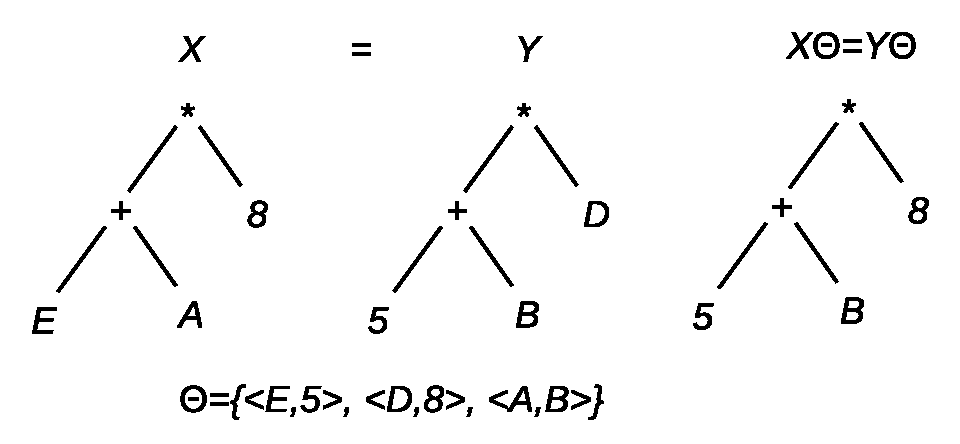
\includegraphics[scale=0.5]{pics/unification.eps}
\end{center}
\caption{Унификация двух арифметических выражений}
\label{pic:unification}
\end{figure}



Рассмотрим правила унификации более подробно. Терм {\tt X} унифицируется с термом {\tt Y} по следующим правилам. Если {\tt Х} и {\tt Y} --- символы или числа, то они унифицируемы, только если они одинаковы. Если {\tt Х} является константой или структурой, а {\tt Y} --- неконкретизированной переменной, то {\tt Х} и {\tt Y} унифицируемы и {\tt Y} принимает значение {\tt Х} (и наоборот). Если {\tt Х} и {\tt Y} --- структуры, то они унифицируемы тогда и только тогда, когда у них один и тот же главный функтор и арность и каждая из их соответствующих компонент сопоставима. Если {\tt Х} и {\tt Y} --- неконкретизированные (свободные) переменные, то они сопоставимы, в этом случае говорят, что они сцеплены. В табл.~\ref{tab:unif} приведены примеры унифицируемых и неунифицируемых термов.

\begin{table}[ht]
\caption{Иллюстрация унификации} \label{tab:unif}
\begin{center}\tt
\begin{tabular}{|l|l|l|}
 \hline
 {\rm Терм${}_1$} & {\rm Терм${}_2$}  &  {\rm Унифицируемы?}
 \\\hline\hline
 jack(Х)  &  jack(human) & {\rm да:} Х=human
 \\\hline
 jack(person) & jack(human)  &  {\rm нет}
 \\\hline
 jack(Х, Х) & jack(23, 23)  &  {\rm да:} Х=23
 \\\hline
 jack(Х, Х) & jack(12, 23)  &  {\rm нет}
 \\\hline
 jack(\_, \_) & jack(12, 23)  &  {\rm да}
 \\\hline
 f(Y, Z) & X  &  {\rm да:} X = f(Y, Z)
  \\\hline
 X & Z  &  {\rm да:} X = Z
  \\\hline
\end{tabular}
\end{center}
\end{table}

Следует сказать, что в большинстве реализаций Пролога для повышения эффективности его работы допускается существование циклических унификаторов\footnote{Унификация без проверки вхождения терма имеет сложность $O(n)$, тогда как строгая --- $O(n^2)$.}. Например, попытка унифицировать термы {\tt f(X)} и {\tt Х} приведет к циклической подстановке {\tt X = f(X)}, который определяет бесконечно-вложенный терм {\tt f(f(f(...)))}, что еще и логически некорректно. Иногда такую неполную унификацию называют мэтчинг (matching).

Возможность унификации (мэтчинга)) двух термов проверяется с помощью оператора <<{\tt =}>>.

Ответом на запрос
{\tt\begin{verbatim}
    3 + 2 = 5
\end{verbatim}}
\noindent в ISO-Prolog будет {\tt нет}, так как термы неунифицируемы (в ISO-Prolog оператор <<{\tt =}>> не вычисляет значения своих аргументов). ISO-Prolog воспринимает арифметические операции как функторы, а арифметические выражения --- как сложные структуры; для вычисления арифметических выражений используется специальный предикат <<{\tt is}>>. % Но, к примеру, Visual Prolog вычислит значение без использования <<{\tt is}>>.

Унификация часто используется для доступа к подкомпонентам термов. Так, например, если нам требуется выбрать правое поддерево (см. пример~\ref{ex:treesearch}), можно провести следующую унификацию ({\tt T} --- исходное дерево, {\tt ST} --- поддерево).
{\tt\begin{verbatim}
    T=t( t( nil, 7, nil), 5, t( t(nil, 10, nil), 8,
        nil)),
    ( _, _, ST) = T
        % теперь ST = t( t(nil, 10, nil), 8, nil).
\end{verbatim}}

Отрицание оператора <<{\tt =}>> записывается как <<{\tt \verb|\=|}>> или <<{\tt \verb|\+| (\_ = \_)}>>.

\section{Лабораторная работа 1: Факты и правила}

Формализация высказываний естественного языка в виде Про\-лог-прог\-рам\-мы.

\paragraph{Задание.} В pаботе\footnote{Задание на лабораторную работу 1 разработано преподавателем кафедры вычислительной техники Института кибернетики НИ ИрГТУ, доцентом, канд.~техн.~наук С.~С.~Сосинской.} тpебуется формализовать высказывания в виде программы на языке Пpолог. В программе требуется выполнить ряд запросов, объяснить выдаваемые системой результаты.

\paragraph{Цель работы.} Приобрести навыки формализации высказываний на естественном языке в виде фактов, правил и запросов языка Пролог.

\paragraph{Время работы.} На выполнение работы отводится два академических часа.

\paragraph{Индивидуальные задания}
\begin{enumerate}
\item Флэш --- собака. Pовеp --- собака. Бутси --- кошка. Стаp --- лошадь.
    Флэш чеpная. Бутси коpичневая. Pевеp pыжая. Стаp белая.
    Домашнее животное --- собака или кошка.
    Животное --- домашнее животное или лошадь.
    У Тома есть собака не чеpного цвета.
    У Кейта есть лошадь или что-то чеpного цвета.\\{}
    \textbf{Запросы}:\begin{itemize}
    \item Pовеp рыжая?
    \item Опpеделить клички всех собак.
    \item Опpеделить владельцев чего-либо.
    \item Опpеделить владельцев животных небелого цвета.
    \end {itemize}
 \item Бутси --- коpичневая кошка. Коpни --- чеpная кошка.
 Мактэвити --- pыжая кошка.
    Флэш, Pовеp и Спот --- собаки; Pовеp --- pыжая, а Спот --- белая.
    Все животные, котоpыми владеют Том и Кейт, имеют pодословные.
    Том владеет всеми чеpными и коpичневыми животными.
    Кейт владеет всеми собаками небелого цвета, котоpые не являются
    собственностью Тома.

    Алан владеет Мактэвити, если Кейт не владеет Бутси и если Спот не
    имеет pодословной. Флэш --- пятнистая собака.\\{}
        \textbf{Запросы}:\begin{itemize}
             \item Какие животные не имеют хозяев?
             \item Найдите всех собак и укажите их цвет.
             \item Укажите всех животных, котоpыми владеет Том.
             \item Пеpечислите всех собак Кейта.
        \end{itemize}
 \item Опpеделить следующие отношения: СЫH, ДОЧЬ, ОТЕЦ, \linebreak{}МАТЬ, МУЖЧИHА и ЖЕHЩИHА.
    Описать факты для некотоpых из них.\\{}
        \textbf{Запросы}:\begin{itemize}
             \item Опpеделить всех сыновей опpеделенной матеpи.
             \item Опpеделить всех детей опpеделенной паpы pодителей.
             \item Опpеделить pодителей опpеделенного человека.
             \item Является ли опpеделенный человек женщиной?
        \end{itemize}
 \item Мэpи любит пеpсики. Мэpи любит кукуpузу. Мэpи любит яблоки.
    Бет любит то, что любит Мэpи, если это --- фpукт и если он кpасный.
    Бет любит то, что любит Мэpи, если это кукуpуза.
    Пеpсики --- фpукт. Яблоки --- фрукт.
    Цвет пеpсиков желтый. Цвет апельсинов оpанжевый. Цвет яблок кpасный.
    Цвет яблок желтый.\\{}
    \textbf{Запросы}:\begin{itemize}
             \item Что любит Бет?
             \item Любит ли Мэpи кукуpузу?
             \item Какие фpукты известны?
             \item Какого цвета фpукты, котоpые любят Бет и Мэpи?
    \end{itemize}
\item Задано деpево pодственных связей.

\begin{minipage}[b]{.4\linewidth}
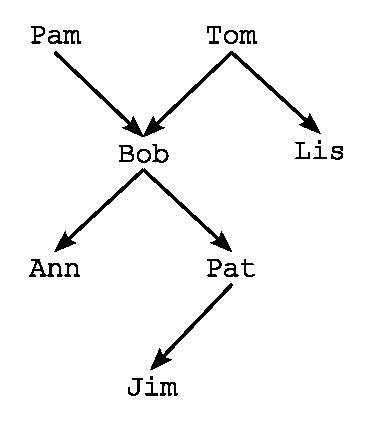
\includegraphics[scale=0.7]{pics/task_relatives.eps}
\end{minipage}
\begin{minipage}[b]{.6\linewidth}Кpоме того, опpеделить отношения
             ПОЛ, PЕБЕHОК, PОДИТЕЛЬ\_PОДИТЕЛЯ, ПРЕДОК и
              МАТЬ.\\{}
            \textbf{Запросы}:
            \begin{itemize}
              \item Кто pодитель Pat?
             \item Есть ли у Lis pебенок?
              \item Кто потомки Pat?
             \item Является ли Pam матеpью Bob?
             \end{itemize}
\end{minipage}
\item Медведь большой. Слон большой. Кот маленький. Медведь коpичневый.
    Кот чеpный. Слон серый.

    \noindent Любой черный или коричневый пpедмет является темным.\\{}
    \textbf{Запросы}:\begin{itemize}
            \item Кто одновpеменно большой и темный?
            \item Есть ли коpичневые маленькие слоны?
            \item Есть ли большие и темные медведи?
            \item Есть ли чеpный кот?
    \end{itemize}
\item Мэpи, Сьюзи и Джейн pаботают в дневную смену. Сэм, Джейн, Боб и Патpиция
    pаботают в вечеpнюю смену. Знают дpуг дpуга те, кто pаботает в одну смену.\\{}
    \textbf{Запросы}:\begin{itemize}
            \item Знают ли дpуг дpуга Мэpи и Джейн?
            \item  Кто pаботает в дневную смену?
            \item  Есть ли кто-то, кто pаботает в обе смены?
            \item  Есть ли кто-то, кто не знает дpуг друга?
    \end{itemize}
\item  Можно совеpшить путешествия, перечисленные в табл.~\ref{tbl:schedule}.

\begin{table}
\caption{Расписание рейсов}\label{tbl:schedule}
\centering
\begin{tabular}{|llll|}
    \hline
       Компания  &  Из    &     В   &       Вид транспорта\\
    \hline\hline

        Амтpак   &  Hью-Йоpк  & Бостон   &  Ж/д\\
        \hline
        Тpанзит   & Hью-Йоpк &  Пpинстон  & Ж/д\\
        \hline
        Амтpак  &   Бостон    & Поpтленд  & Ж/д\\
        \hline
        Гpейхаунд & Бостон   &  Поpтленд  & Автобус\\
        \hline
        Амтpак  &   Hью-Йоpк  & Вашингтон & Ж/д\\
        \hline
        Пиплз    &  Hью-Йоpк  & Вашингтон & Самолет\\
        \hline
        Пиплз    &  Биpлингтон & Hью-Йоpк  & Самолет\\
        \hline
\end{tabular}
\end{table}
   Любые две тpанспоpтные компании являются конкуpентами, если они обслуживают
   один и тот же маршрут.
   Можно путешествовать из одного гоpода в дpугой, если возможно путешествие
   из одного гоpода в дpугой чеpез пpомежуточный (тpетий) город.\\{}
   \textbf{Запросы}:\begin{itemize}
           \item Являются ли Амтpак и Пиплз конкуpентами?
            \item Какие компании дают возможность путешествовать из\linebreak{} Hью-Йоpка
            в Вашингтон?
            \item Можно ли путешествовать из Биpлингтона в Поpтленд?
            \item Опpеделить всех конкуpентов.
    \end{itemize}
\item Опpеделить факты о пpинадлежности студента опpеделенной студенческой
    гpуппе. Считается, что два студента знают дpуг дpуга, если они учатся
    в одной группе.\\{}
    \textbf{Запросы}:\begin{itemize}
            \item Кого знает опpеделенный студент?
            \item  Опpеделить состав опpеделенной гpуппы.
            \item  В каких гpуппах учатся люди с опpеделенным именем?
            \item  Знает ли один студент другого?
    \end{itemize}
\item Имеются факты о маpшpутах движения автобусов между двумя pазными
    гоpодами, в котоpых указаны: номеp маpшpута, названия двух гоpодов,
    день и вpемя отпpавления и пpибытия. Известны также фамилии водителей,
    pаботающих на опpеделенных маpшpутах. Можно попасть из одного гоpода в
    дpугой, если существуют автобусные маpшpуты из пеpвого гоpода во втоpой
    или из пеpвого гоpода в пpомежуточный, и из пpомежуточного во втоpой
    (пpичем подходят и дни, и часы отправления).\\{}
    \textbf{Запросы}:\begin{itemize}
            \item Можно ли пpоехать из одного гоpода в дpугой?
             \item Указать автобусы, выходящие из опpеделенного гоpода в
             опpеделенный день, и вpемя отпpавления.
             \item Пеpечислить фамилии водителей опpеделенного маpшpута.
             \item Указать дни и часы отпpавления опpеделенного маpшpута.
    \end{itemize}
\item Есть факты об отцах некотоpых людей и о бpатьях некотоpых людей.
    Опpеделить отношение ДЯДЯ.\\{}
    \textbf{Запросы}:\begin{itemize}
            \item Опpеделить бpатьев конкpетного человека.
             \item Кто является отцом конкретного лица?
             \item Связаны ли два человека отношением ОТЕЦ?
             \item Опpеделить, является ли один человек дядей другого.
    \end{itemize}
\item Опpеделить отношения PОДИТЕЛЬ, ЖЕHЩИHА как набоp фактов, пpавило
    PАЗЛИЧHЫ, СЕСТPА (опpеделяемое чеpез PОДИТЕЛЬ, ЖЕНЩИНА и PАЗЛИЧHЫ) и
    ТЕТЯ (опpеделяемое чеpез PОДИТЕЛЬ и СЕСТРА).\\{}
    \textbf{Запросы}:\begin{itemize}
            \item Кто является pодителями опpеделенного человека?
             \item Опpеделить всех детей опpеделенных pодителей.
             \item Опpеделить, есть ли сестpы у опpеделенного человека.
             \item Опpеделить, есть ли тетя у опpеделенного человека.
    \end{itemize}
\end {enumerate}

\subsubsection*{Методические указания к выполнению лабораторной работы}
\indent{}Процесс построения некоторого формального представления высказываний естественного языка называется {\em формализацией}. Что это такое? Ответ на этот вопрос столь сложен, сколь сложен ответ на вопрос: Что такое модель? В научных кругах под формализацией понимается словосочетание <<дружеский шарж>>, т.~е. формальное представление некоторого естественного объекта (например, высказывания) --- это дружеский шарж.

Продемонстрируем на примерах, почему формализация --- это именно {\bf шарж}. Пусть дано высказывание: <<Лена любит кататься на велосипеде и на горных лыжах>>. Какая логическая связка будет соответствовать союзу <<и>>?\ldots На самом деле это будет связка <<$\vee$>>, потому, что с формально-логической точки зрения высказывание обозначает: <<Лена катается на велосипеде {\bf или} горных лыжах>>. Второй пример: <<Я пойду домой, а моя жена на работу>>. Здесь союз <<а>> по смыслу соответствует логической связке <<\&>>. Таким образом, формализация естественного текста не может быть сделана <<в лоб>>, необходимо понять, что было сказано.

При выполнении лабораторной работы следует придерживаться следующих общих правил:
\begin{enumerate}
\item Прочитать весь текст высказывания и определить, что будет {\bf объектами}, а что {\bf свойствами}, связывающими эти объекты. Например, пусть даны следующие высказывания: <<Аня любит Колю. Коля любит Лену. А Лена смотрит в светлое будущее.>> Тогда, объектами будут: Аня, Коля, Лена и <<светлое будущее>>, а свойствами --- отношения <<любит>> и <<смотреть в>>, которые связывают два объекта (<<Кто>> <<любит>>
<<Что>>\footnote{См. замечательный интенсивный курс перевода с английского языка Милошевича.}, <<Кто>> <<смотрит в>> <<Что>>).
\item Свойства объектов могут быть заданы перечислением либо через другие известные свойства. В нашем примере свойство <<любит>> задается перечислением:
{\tt\begin{verbatim}
 be_in_love(ann, niko).
 be_in_love(niko, helen).
\end{verbatim}}
\noindent Но высказывание, вроде <<любовного треугольника>>, можно задать через {\tt be\_in\_love/2}:
{\tt\begin{verbatim}
 love_triangle(X, Y, Z) :-
                      % любовный треугольник
    be_in_love(X, Y),   % первого рода, когда
    be_in_love(Z, Y).   % двое любят одного.
 love_triangle(X, Y, Z) :-
                      % любовный треугольник
    be_in_love(X, Y),  % второго рода - без-
    be_in_love(Y, Z).  % ответная любовь.
\end{verbatim}}
\end{enumerate}

Признаком хорошей формализации (дружественности шаржа) является, как и везде в программировании, хорошая гибкость и интерпретируемость программы: более сложные отношения формулируются через более простые; свойства в достаточной мере абстрактны.

\begin{questions}
\item{} Какие структурные единицы формируют программу на языке Пролог?
\item{} Перечислите простые структуры данных Пролога.
\item{} Что такое <<терм>>, в чем отличие переменной от символа?
\item{} Приведите пример унификации двух структур, представляющих логические выражения.
\item{} Какова будет унифицирующая подстановка $\Theta$ двух следующих термов: \texttt{X=fib(Y+1)} и \texttt{Y=fib(C+5+D)}\footnote{\texttt{Y=fib((C+5)+D)}.}?
\end{questions}

\chapter{Списки и их обработка}

Кроме описанных в разделе \ref{sec:complex_data} структур данных, создаваемых с помощью функторов, в Прологе существует еще одна структура данных --- {\em список}.

\paragraph{Списковая форма записи.} Задачи, связанные с обработкой списков, на практике встречаются очень часто. Скажем, нам понадобилось составить список студентов, находящихся в аудитории. С помощью Пролога мы можем определить список как последовательность термов, заключенных в скобки. Приведем примеры правильно построенных списков Пролога:

{\tt\begin{verbatim}
    [jack, john, fred, jill, john]
    [name(john, smith), age(jack, 24), X]
    [Х, У, date(12, january, 1986), Х]
    []
\end{verbatim}}
\noindent В Turbo Prolog структура списков должна быть определена в явном виде в секции {\tt Domains}. Например, список, состоящий из строковых значений, определяется в Turbo Prolog так:
{\tt\begin{verbatim}
    Domains
        str_list = string *
\end{verbatim}}
\noindent Символ <<{\tt *}>> определяет свойство нового типа {\tt str\_list} <<быть списком>> строк.

Запись {\tt [H | T]} определяет список, полученный добавлением элемента (терма) {\tt Н} в начало списка {\tt Т}. Говорят, что {\tt Н} --- голова, а {\tt Т} --- хвост списка {\tt [H | T]}. На запрос
{\tt\begin{verbatim}
| ?- L = [a | [b, c, d]].
\end{verbatim}}
\noindent будет получен ответ
{\tt\begin{verbatim}
    L = [a, b, c, d],
\end{verbatim}}
\noindent а на запрос
{\tt\begin{verbatim}
| ?- L = [a, b, c, d], L2 = [2 | L].
\end{verbatim}}
\noindent --- ответ
{\tt\begin{verbatim}
    L = [a, b, c, d], L2 = [2, a, b, c, d].
\end{verbatim}}

Запись {\tt [Н | Т]} используется для того, чтобы определить голову и хвост списка. Так, запрос
{\tt\begin{verbatim}
    [X | Y] = [a, b, c].
\end{verbatim}}
\noindent дает ответ
{\tt\begin{verbatim}
    Х = а, Y = [b, c].
\end{verbatim}}

Заметим, что употребление только имен переменных {\tt Н} и {\tt Т} необязательно. Кроме записи вида {\tt [H | T]}, для выборки термов используются переменные. Запрос
{\tt\begin{verbatim}
| ?- [a, X, Y] = [a, b, c].
\end{verbatim}}
\noindent определит значения
{\tt\begin{verbatim}
    X=b, Y=c,
\end{verbatim}}
\noindent а запрос
{\tt\begin{verbatim}
| ?- [person(Х) | Т] = [person(john), а, b].
\end{verbatim}}
\noindent значения
{\tt\begin{verbatim}
    Х=john, Т=[а, b].
\end{verbatim}}

Можно отделять в качестве головы несколько элементов, соответствующая запись будет выглядеть так: {\tt L = [X1, X2, X3 | T]}.

\paragraph{Некоторые стандартные отношения для обработки списков.} Покажем на примерах использование записи вида {\tt [Н | T]} вместе с рекурсией для определения некоторых полезных отношений над списками.

\emph{Принадлежность элемента списку}. Сформулируем задачу проверки принадлежности данного терма списку\footnote{Используется методика рассуждения, представленная в книге \cite{Bratko}. Сначала рассматриваются самые простые варианты входных данных, затем сложные.}.

\begin{quote}
\noindent Граничное условие (база индукции): Терм {\tt R} содержится в списке {\tt [H | T]}, если {\tt R = H}.\\
Рекурсивное условие (индуктивный шаг): Терм {\tt R} содержится в списке {\tt [H | T]}, если {\tt R}
содержится в списке {\tt Т}.
\end{quote}

\noindent Первый вариант записи определения на Прологе имеет вид:
{\tt\begin{verbatim}
    in(R, L) :-
        L=[H | T], H=R.
    in(R, L) :-
        L=[H | T], in(R, T).
\end{verbatim}}

\noindent Цель {\tt L = [H | T]} в теле обоих утверждений служит для того, чтобы разделить список {\tt L} на голову и хвост.

Можно улучшить программу, если учесть тот факт, что Пролог сначала унифицирует с целью голову утверждения, а затем пытается унифицировать его тело. Новая процедура {\tt in} определяется таким образом:
{\tt\begin{verbatim}
    in(R, [R | Т]).
    in(R, [H | Т]) :- in(R, T).
\end{verbatim}}

\noindent На запрос
{\tt\begin{verbatim}
| ?- in(а, [а, b, с]).
\end{verbatim}}
\noindent будет получен ответ {\tt yes}.
\noindent На запрос
{\tt\begin{verbatim}
| ?- in(b, [a, b, с]).
\end{verbatim}}
\noindent тоже ответ {\tt yes}.

Существуют реализации Пролога, где предикат {\tt принадлежит} ({\tt in}) является встроенным, например, в ISO-Prolog этот предикат называется \texttt{member/2}.

\emph{Соединение двух списков}. Задача присоединения списка {\tt Q} к списку {\tt Р}, в результате чего получается список {\tt R}, формулируется следующим образом:
\begin{quote}
\noindent Граничное условие: Присоединение к {\tt []} списка {\tt Q} дает {\tt Q}.
\noindent Рекурсивное условие: Присоединение к концу списка {\tt Р} списка {\tt Q} выполняется так: {\tt Q} присоединяется к хвосту {\tt Р}, а затем спереди добавляется голова {\tt Р}.
\end{quote}

Определение (см. рис.~\ref{pic:list_descr}) можно непосредственно записать на Прологе:
{\tt\begin{verbatim}
    conc([], Q, Q).
    conc(Р, Q, R) :-
        Р=[НР | ТР],
        conc(TP, Q, TR),
        R=[HP | TR].
\end{verbatim}}

\begin{figure}[hbt]
\begin{center}
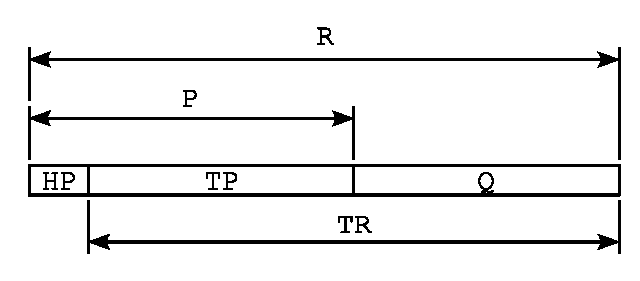
\includegraphics[scale=0.7]{pics/list_descr.eps}
\end{center}
\caption{Конкатенация списков {\tt [HP | TP]}, {\tt Q}, {\tt [HP | TR]}}
\label{pic:list_descr}
\end{figure}

\noindent Однако, как и в предыдущем примере, воспользуемся тем, что Пролог унифицирует с целью голову утверждения, прежде чем пытаться согласовать тело:
{\tt\begin{verbatim}
    conc([], Q, Q).
    conc([HP | TP], Q, [HP | TR]) :-
        conc(TP, Q, TR).
\end{verbatim}}
\noindent На запрос
{\tt\begin{verbatim}
| ?- conc([а, b, с], [d, e], L).
\end{verbatim}}

\noindent будет получен ответ
{\tt\begin{verbatim}
    L = [a, b, c, d],
\end{verbatim}}
\noindent но на запрос
{\tt\begin{verbatim}
| ?- conc([a, b], [c, d], [e, f]).
\end{verbatim}}
\noindent ответом будет {\tt no}.

Часто процедура <<присоединить>> используется для получения списков, находящихся слева и справа от данного элемента:
{\tt\begin{verbatim}
| ?- conc(L, [jim | R], [jack, bill, jim,
        tim, jim, bob]).
    L = [jack, bill], R = [tim, jim, bob];
    % далее идет еще одно решение
    L=[jack, bill, jim, tim], R=[bob].
\end{verbatim}}
В командной строке GNU-Prolog при выполнении запроса и при наличии множества решений интерпретатор, выдав очередное решение, приостанавливает процесс решения задачи и ожидает реакцию пользователя на незримый вопрос <<Что делать дальше --- остановить процесс поиска решения, вывести новое решение, вывести все решения?>> Если вам достаточно одного решения, то, нажимая клавишу <<Enter>>, вы вернетесь в командную строку запроса. Если вас интересует еще одно решение, то при нажатии клавиши <<;>> Пролог попытается найти это решение. GNU-Prolog позволяет вывести все решения, для этого предназначена клавиша <<a>>\footnote{Латинская маленькая буква <<a>>.} (all). Некоторые задачи могут порождать бесконечное количество решений. Остановка процесса бесконечного порождения решений и <<зациклившейся>> программы осуществляется нажатием комбинации <<Ctrl-C>> и выполнением команды отладчика <<a>> (abort).

Вот еще один пример использования процедуры <<присоединить>>. Здесь производится разрезание списка на два подсписка всеми возможными способами:
{\tt\begin{verbatim}
| ?- conc(L, R, [jack, bill, jim, tim, jim, bob]).
    L = [], R = [jack, bill, jim, tim, jim, bob];
    L = [jack], R = [bill, jim, tim, jim, bob];
    L = [jack, bill], R = [jim, tim, jim, bob];
    L = [jack, bill, jim], R = [tim, jim, bob];
    L = [jack, bill, jim, tim], R = [jim, bob];
    L = [jack, bill, jim, tim, jim], R = [bob];
    L = [jack, bill, jim, tim, jim, bob], R = [].
\end{verbatim}}
Необходимо заметить, что многие прологовские программы могут быть использованы как по прямому назначению, так и в обратном направлении. В этом, в частности, состоит сила логического программирования.

\emph{Индексирование списка}. Задача получения $N$-гo терма в списке определяется следующим образом:

\begin{quote}
\noindent Граничное условие: Первый терм в списке {\tt [Н | Т]} есть {\tt Н}.

\noindent Рекурсивное условие: $N$-й терм в списке {\tt [Н | Т]} является $(N-1)$-м термом в списке {\tt Т}.
\end{quote}

Данному определению соответствует программа:

{\tt\begin{verbatim}
    get([H | Т], 1, Н). % Граничное условие
    get([Н | Т], N, Y) :- % Рекурсивное условие
        М is N - 1,
        get(Т, М, Y).
\end{verbatim}}

\emph{Принадлежность одного списка другому} можно проверить с помощью разбиений:

\begin{quote}
    Список {\tt S} является подсписком {\tt L}, если {\tt L} можно разбить на два списка {\tt L1} и {\tt L2}, и {\tt L2} можно разбить на два списка {\tt S} и {\tt L3}.
\end{quote}

\begin{figure}[hbt]
\begin{center}
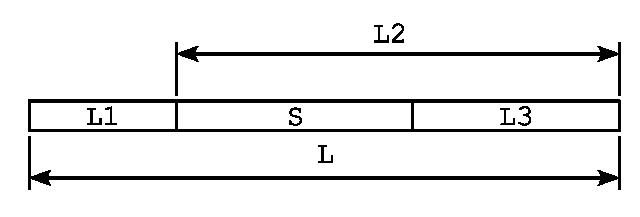
\includegraphics[scale=0.7]{pics/list_inc.eps}
\end{center}
\caption{Отношение <<подсписок>> {\tt sublist/2}.}
\label{pic:list_inc}
\end{figure}

{\tt\begin{verbatim}
    sublist(L, S) :-
        conc(L1, L2, L),
        conc(S, L3, L2).
            % Вместо L3 можно подставить "_".
\end{verbatim}}


\emph {Пеpестановки списка.}

\begin{quote}
     \noindent Если исходный список пуст, то и пеpестановка этого списка --- пустой список.
     \noindent Если исходный список не пуст, то следует получить пеpестановку хвоста {\tt L} этого списка, и затем добавить голову {\tt X} списка к полученному списку.
\end{quote}

\rem{
\begin{figure}[hbt]
\begin{center}
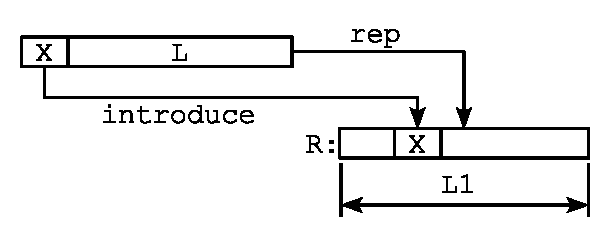
\includegraphics[scale=0.7]{pics/list_rep.eps}
\end{center}
\caption{Отношение <<перестановка>> {\tt rep/2}.}
\label{pic:list_rep}
\end{figure}
}

{\tt\begin{verbatim}
    rep([], [])
    rep([X | L], R) :-
        rep(L, L1),
        introduce(X, L1, R).
    introduce(X, [X | L]).      % ... "в голову"
    introduce(X, [Y | L]) :-    % ... в хвост.
        introduce(X, L).
\end{verbatim}}

\paragraph{Сортировка списков.} Рассмотрим несколько методов сортировки списков.

\emph{Соpтиpовка списка методом пузыpька}. Для упоpядочения списка {\tt С} необходимо:
\begin{quote}
       \noindent Hайти в {\tt С} два смежных элемента {\tt Х} и {\tt Y} таких,
       что {\tt Х~>~Y}, и поменять их
       местами;

       \noindent Если в {\tt С} нет ни одной паpы смежных элементов
       {\tt Х} и {\tt Y} таких, что {\tt Х~>~Y},
       то считать, что {\tt С} уже отсоpтиpован.
\end{quote}

{\tt\begin{verbatim}
    buble_sort(L1, L2) :-
        exchange_one(L1, L3), !,
        buble_sort(L3, L2).
    buble_sort(L, L).

    exchange_one([X, Y | T], [Y, X | T]) :-
        X > Y.
    exchange_one([X, Y | T], [X | R]) :-
        \+ X > Y,
        exchange_one([Y | T], R).
\end{verbatim}}

\emph{Соpтиpовка списка методом вставки.} Для упоpядочения списка {\tt С} необходимо:
\begin{quote}
        \noindent Пустой список считаем упорядоченным.

       \noindent Упоpядочить хвост списка {\tt С}.

       \noindent Вставить голову списка {\tt С} в упоpядоченный хвост, поместив ее в такое место, чтобы получившийся список остался упорядоченным.
\end{quote}
\noindent Программу приводить не будем, оставим это как упражнение.

\emph{Быстpая соpтиpовка списка.}

     Для упоpядочения списка {\tt С} необходимо:
\begin{quote}
        \noindent Пустой список считаем упорядоченным.

       \noindent Удалить из списка пеpвый элемент {\tt Х} и pазбить оставшуюся часть на два списка: {\tt L} --- с элементами, меньшими {\tt X}, и {\tt M} --- со всеми остальными элементами.

       \noindent Упоpядочить список {\tt L} с получением списка {\tt SL}.

       \noindent Упоpядочить список {\tt M} с получением списка {\tt SM}.

       \noindent Получить pезультиpующий упоpядоченный список {\tt SC} как объединение {\tt SL}, {\tt Х} и {\tt SM}.
\end{quote}

\noindent
       Hапpимеp,  исходный список {\tt С = [5, 3, 7, 8, 1, 4, 7, 6]}. \\ Удаляем {\tt Х = 5}.\\
       Список {\tt [3, 7, 8, 1, 4, 7, 6]} разбиваем на два:\\ {\tt L = [3, 1, 4]};  {\tt M = [7, 8, 7, 6]}.\\
       Соpтиpуем последние списки, получаем:\\ {\tt SL = [1, 3, 4]}; {\tt SM = [6, 7, 7, 8]}.\\
       Результат {\tt SC} получаем объединением {\tt SL} и {\tt [X | SM]}.\\
       Итак, {\tt SC = [1, 3, 4, 5, 6, 7, 7, 8]}.

{\tt\begin{verbatim}
    quick_sort([], []).
    quick_sort([X | T], SC):-
        distrib(T, X, L, M),
        quick_sort(L, SL),
        quick_sort(M, SM),
        conc(SL, [X | SM],SC).
    distrib([], _, [], []).
    distrib([H | T], X, [H | T1], L) :-
        X > H, distrib(T, T1, L).
    distrib([H | T], X, L, [H | T1]) :-
        \+ X > H, distrib(T, L, T1).
\end{verbatim}}

\paragraph{Построение списков из фактов.} Иногда бывает полезно представить в виде списка информацию, содержащуюся в известных фактах. В большинстве реализаций Пролога есть необходимые для этого предикаты:
\begin{description}
\item[\normalfont\tt bagof(X, Y, L)] определяет список термов {\tt L}, конкретизирующих переменную {\tt Х} как аргумент предиката {\tt Y}, которые делают истинным предикат {\tt Y}.

\item[\normalfont\tt setof(X, Y, L)] все сказанное о предикате {\tt bagof} относится и к {\tt setof}, за исключением того, что список {\tt L} отсортирован и из него удалены все повторения.

\item[\normalfont\tt findall(X, Y, L)] все сказанное о предикате {\tt bagof} относится и к {\tt findall}, за исключением того, что список {\tt L} может быть пустым, если нет ни одного истинного предиката {\tt Y}. Предикат {\tt findall/3} всегда истинный.
\end{description}
%Замечание: В Turbo-Прологе перечисленные предикаты работают со всеми, определенными в программе в секции {\tt Domains} списками (для {\tt L}).

Если имеются факты:

{\tt\begin{verbatim}
    dog(rex).
    dog(goldy).
    dog(fido).
    dog(reke).
    dog(fido).
\end{verbatim}}

\noindent то на запрос

{\tt\begin{verbatim}
| ?- bagof(D, dog(D), L),
\end{verbatim}}

\noindent так же как и для {\tt findall/3}, будет получен ответ
{\tt\begin{verbatim}
    L = [rex, goldy, fido, reke, fido],
\end{verbatim}}

\noindent в то время как

{\tt\begin{verbatim}
| ?- setof(D, dog(D), L)
\end{verbatim}}

\noindent дает значение
{\tt\begin{verbatim}
    L = [fido, goldy, reke, rex].
\end{verbatim}}

\noindent На запрос
{\tt\begin{verbatim}
    findall(D, cat(D), L)
\end{verbatim}}

\noindent ответом будет
{\tt\begin{verbatim}
    L = [],
\end{verbatim}}
\noindent а подобные запросы {\tt bagof/3} и {\tt setof/3} завершились бы неудачей.

\section{Грамматический разбор текста}

Пролог обладает большими возможностями по сопоставлению объектов с эталоном\footnote{Англоязычный вариант термина --- pattern matching.}, поэтому данный язык программирования хорошо подходит для обработки текстов \cite{Malpas}. На Прологе можно с успехом реализовать генераторы отчетов, текстовые редакторы и трансляторы с различных языков. В данном разделе рассматриваются программы, предназначенные для обработки текстов. На примере этих программ демонстрируется непосредственное практическое применение систем Пролог.

Действия, выполняемые программой обработки текстов, разбиваются на две фазы. В течение первой фазы, называемой \emph{лексическим анализом}, входной текст преобразуется из внешней формы в некоторое внутреннее представление. Во время второй фазы выполняется анализ или тот или иной вид обработки внутреннего представления текста. \emph{Система грамматического разбора} --- это процедура, которая распознает синтаксические структуры высокого уровня (объекты) во внутреннем представлении текста.

\subsection{Стратегии грамматического разбора}

Одна из причин, по которой системы грамматического разбора вызывают столь большой интерес, заключается в существовании близкой аналогии между \emph{стратегиями грамматического разбора} и \emph{стратегиями решения задач} в целом. В интерпретаторе языка Пролог по умолчанию принята стратегия решения задач с \emph{обратным ходом решения}. Решение начинается с гипотезы (т.~е. с запроса), которая затем разбивается на субгипотезы (т.~е. подцели правила), далее каждая субгипотеза делится на еще более мелкие составные части и т.~д. Исходная гипотеза будет подтверждена, когда интерпретатор дойдет до субгипотез, которые уже нельзя разделить на составные части (т.~е. до фактов). Альтернативой служит стратегия решения задач с \emph{прямым ходом решения.} Такая стратегия применяется в языках OPS-5 и CLIPS. Решение начинается с фактов, а затем отыскиваются заключения, вытекающие из них. Далее на основании этих заключений делаются заключения более высокого уровня и т.~д. Это происходит до тех пор, пока не будет достигнуто искомое заключение.

Система нисходящего грамматического разбора базируется (как и Пролог) на стратегии с обратным ходом решения, а система восходящего разбора --- на стратегии с прямым ходом решения (как и язык OPS-5). Вообще говоря, нисходящий грамматический разбор более эффективен, чем восходящий, но существуют некоторые грамматические конструкции, разбор которых можно реализовать только восходящим методом. Поскольку сам Пролог основывается на стратегии с обратным ходом решения, реализация на Прологе систем нисходящего грамматического разбора может быть осуществлена достаточно прямолинейным способом. Реализация восходящего грамматического разбора немного сложнее, так как для применения стратегии с прямым ходом решения требуется процедурная трактовка языка Пролог. Существует также ряд других задач, для которых более предпочтительно использование стратегии с прямым ходом решения.

\subsection{Лексический анализатор}

Лексический анализатор распознает сочетания символов, поступающих из входного потока, и вырабатывает поток лексем. Каждая лексема представляет одну из строк символов. Множество лексем, сгенерированных лексическим анализатором, образует внутреннее представление входного потока (рис.~\ref{pic:lex_anal}).

\begin{figure}[htbp]
\begin{center}

\includegraphics[scale=0.7]{pics/lex_anal.eps}
\end{center}
\caption{Лексический анализатор}\label{pic:lex_anal}
\end{figure}

\subsubsection{Реализация лексического анализатора}

%Пока не нагуглил фронттокен, наверное надо будет его ввести.

Реализация лексического транслятора проще всего представляется в Visual-Prolog. В этом Прологе есть предикат  {\tt fronttoken/3}, который отделяет разделяет входную строку на некоторую лексему и оставшуюся часть строки. Лексемы --- это либо числа, либо знаки, либо слова, разделенные пробелами.
{\tt\begin{verbatim}
    lex(Str, [Tok | Tokens]) :-
        fronttoken(Str, Tok, RStr), !,
        lex(RStr, Tokens).
    lex(S, []).  % Для пустых строк.
\end{verbatim}}
\noindent Теперь {\tt lex/2} будет истинным по определению, если строка {\tt Str} разбивается на список лексем {\tt [Tok | Tokens]} по правилам предиката {\tt fronttoken/3}.

В стандарте ISO есть предикат \texttt{read\_token/2}, который считывает лексему из входного потока, например, файла или специальным образом ассоциированного с потоком атома (строки).
{\tt\begin{verbatim}
    lex1(Stream, L) :-
        read_token(Stream, Term),!,
        (
            Term=punct(end_of_file), % Конец файла?
            L=[],!; % Да.
            !,      % Нет.
            conv_lex(Term, T), % Убрать разметку.
            lex1(Stream, Tail), % Следующая лексема.
            app(T, Tail, L)    %
        ).
    lex(Atom, L):-
        open_input_atom_stream(Atom, Stream),
        lex1(Stream, L),
        close_input_atom_stream(Stream).
\end{verbatim}}
В этой версии предикат \texttt{lex1/2} --- вспомогательный. Реализация \texttt{lex/2} в SWI-Prolog будет иной.

Проведем испытания нашего лексического анализатора в GNU-Prolog\footnote{В Visual-Prolog запрос остается таким же, но одинарные кавычки надо заменить на двойные.}:
{\tt\begin{verbatim}
| ?- lex('The cow shakes the tail', L).
    L = ['The', 'cow', 'shakes', 'the', 'tail']

    lex('Slithy towes did gyre', L).
    L = ['Slythy', 'towes', 'did', 'gyre']

    lex('The cow jumped over the Moon.', L).
    L = ['The', 'cow', 'jumped', 'over', 'the',
        'Moon', '.']

    lex('FOR I:=1 TO 2013 DO BEGIN END ;', L).
    L = ['FOR', 'I', ':', '=', '1', 'TO', '2013',
        'DO', 'BEGIN', 'END', ';']
\end{verbatim}}
\noindent Видно, что лексический анализатор работает вполне приемлемо.

\subsection{Система нисходящего грамматического разбора}

Система грамматического разбора --- это программа, которая распознает синтаксические объекты в потоке лексем. Здесь описана программа нисходящего грамматического разбора {\tt object/3}. На вход программы поступают список слов и название определенного синтаксического объекта более высокого уровня. Программа разбора добьется успеха, если в начале списка обнаружит слова, из которых формируется требуемый синтаксический объект. В противном случае программа потерпит неудачу. Грамматика для программы {\tt object/3} --- это несложное подмножество английского языка. Распознаваемые программой синтаксические объекты --- это все части предложений английского языка, такие как <<предложение>>, <<глагольная группа>> или <<артикль>>. Программа {\tt object/3} одновременно представляет собой и словарь, и грамматику.

Согласно терминологии грамматического разбора \emph{терминальный символ} (или \emph{терминал}) --- это входная лексема, поступающая из блока синтаксического анализа, а \emph{нетерминальный символ} (или \emph{нетерминал)} --- это синтаксический объект, образованный комбинацией терминальных или нетерминальных символов. Множество терминалов, известное системе разбора, называется ее \emph{словарем}. Компоненты каждого нетерминала специфицируются при помощи \emph{грамматического правила}, а множество грамматических правил, известных системе разбора, образует ее \emph{грамматику}.

В описываемой системе используется простая грамматика, которую можно в схематической форме Бэкуса\,{}-\,{}Наура представить так:
{\tt\begin{verbatim}
    <предложение> ::= <глагольная группа>
        <группа существительного>
    <группа существительного> ::= <артикль>
        <существительное>
    <глагольная группа> ::= <глагол>
        <группа существительного>
\end{verbatim}}

Знак <<{\tt ::=}>> здесь читается как <<состоит из>>. В программе каждый терминал, входящий в состав словаря, представляется фактом {\tt object}, а каждый нетерминал, входящий в грамматику, представляется правилом {\tt object/3}.
{\tt\begin{verbatim}
    % Принятые имена переменных
    % I - входной список лексем
    % О, R - выходной список лексем
    % нетерминалы:

    object(I, О, 'предложение') :-
        object(I, R, 'группа существительного'),
        object(R, О, 'глагольная группа').

    object(I, О, 'группа существительного') :-
        object(I, R, 'артикль'),
        object(R, О, 'существительное').

    object(I, О, 'глагольная группа') :-
        object(I, R, 'глагол'),
        object(R, О, 'группа существительного').

    % терминалы:

    object(['the' | R], R, 'артикль').
    object(['cow' | R], R, 'существительное').
    object(['tail' | R], R, 'существительное').
    object(['shakes' | R], R, 'глагол').
    object(['walks' | R], R, 'глагол').
\end{verbatim}}

\noindent Заметьте,что форма нетерминальных правил {\tt object} в точности соответствует форме грамматических правил.

Современные реализации Пролога содержат в качестве подсистемы транслятор DCG (Definite clause grammars\footnote{Грамматика, построенная на определенных предложениях.}) \cite{WIKI-DCG}.  DCG удобна для представления грамматических правил при создании трансляторов. DCG не входит в стандарт ISO, и поэтому считается, что ее наличие и реализация зависит от системы программирования Пролог. Грамматические правила нашего примера в DCG будут представлены в следующем виде:
{\tt\begin{verbatim}
    % Принятые имена переменных
    % I - входной список лексем
    % О, R - выходной список лексем
    % нетерминалы:

    'предложение' -> 'группа существительного',
        'глагольная группа'.

    'группа существительного' ->
        'артикль', 'существительное'.

    'глагольная группа' -> 'глагол',
        'группа существительного'.

    % терминалы:
    'артикль' -> ['the'].
    'существительное' -> ['cow', 'tail'].
    'глагол' -> ['shakes', 'walks'].
\end{verbatim}}
\noindent{} Такая форма транслируется языком Пролог в представление, аналогичное представлению \texttt{object/3}, только имена правил преобразуются в такие же имена предикатов, добавятся два аргумента \texttt{I, O} (входной и выходной список лексем). Правила DCG могут включать дополнительные аргументы, которые при трансляции будут добавляться в заголовок к \texttt{I, O}. Дополнительные аргументы можно использовать для синтеза необходимых структур, например деревьев синтаксического разбора.

\paragraph{Использование программы {\tt object/3}.} В качестве первого аргумента процедуры {\tt object} передается входной список лексем. Третий аргумент --- это название определяемого объекта. Второй аргумент образован частью списка, остающейся после того, как из начала списка будет взят терминал или нетерминал. Функции аргументов можно проиллюстрировать на примере запроса:

{\tt\begin{verbatim}
| ?- object(['cow', 'horse', 'goat'], Rest,
         'существительное').
     Rest = ['horse', 'goat']
\end{verbatim}}

Запрос спрашивает: <<Можно ли взять {\tt существительное} из начала списка {\tt ['cow', 'horse', 'goat']}, и если да, то какая часть списка останется?>> Ответ на данный запрос показывает, что это возможно и что остается список {\tt ['horse','goat']}. Запрос подтверждает, что слово {\tt cow} является существительным.

Подобным образом, запрос к процедуре {\tt object/3} подтвердит или опровергнет предположение о том, что список слов образует нетерминал:

{\tt\begin{verbatim}
| ?- object(['the', 'cow', '.' ], L,
         'глагольная группа').
     no.

| ?- object(['the', 'cow', '.' ], L,
         'группа существительного').
     L = ['.'] % успех

| ?- object(['the', 'cow', 'shakes', 'the',
         'tail'], L, 'предложение').
     L = [] % успех
\end{verbatim}}

\paragraph{Использование процедуры {\tt object/3} в обратном направлении.}

Все аргументы процедуры {\tt object/3} являются двунаправленными. Это означает, что при помощи запросов к процедуре {\tt object} можно также сгенерировать любые синтаксические объекты, какие только можно построить по входному списку лексем, или даже сгенерировать все возможные предложения по заданным словарю и грамматике.

{\tt\begin{verbatim}
    % проанализировать входной список:
| ?- object(['the', 'tail'], L, Object).    % (1)
     L = ['tail'],
| ?- Object = 'артикль'.
     L = [],
     Object = 'группа существительного'

     % сгенерировать все предложения:
     object(Х, [], 'предложение').    % (2)
     X = ['the', 'cow', 'shakes', 'the', 'cow'];
     X = ['the', 'cow', 'shakes', 'the', 'tail'];
     X = ['the', 'cow', 'walks', 'the', 'cow'];
     X = ['the', 'cow', 'walks', 'the', 'tail'];
     X = ['the', 'tail', 'shakes', 'the', 'cow'];
     X = ['the', 'tail', 'shakes', 'the', 'tail'];
     X = ['the', 'tail', 'walks', 'the', 'cow'];
     X = ['the', 'tail', 'walks', 'the', 'tail'].
\end{verbatim}}

Обратите внимание, что во втором запросе второй аргумент --- {\tt []} указывает, что после окончания грамматического разбора должен остаться пустой список.

Предложения, сгенерированные программе разбора, синтаксически правильны, однако их \emph{семантическая корректность} не гарантируется. Программа может вырабатывать бессмысленные предложения вроде {\tt  ['the', 'cow', 'walks', 'the', 'tail']}, что переводится как 'Корова идет по хвосту'.

Что можно ожидать получить от следующего запроса?
{\tt\begin{verbatim}
| ?- object(А, В, С).
\end{verbatim}}
\begin{questions}
\item{} Пусть \texttt{L=[1, 2, 3, 4]}, \texttt{L=[X1, X2 | Q]}. Каково будет значение \texttt{Q}?
\item{} Справедливо ли высказывание \texttt{[]=[\_|[]]}?
\item{} Каков будет результат выполнения запроса \texttt{findall(X, fail, L)}?
\item{} Дополните программу синтаксического анализа поддержкой не\-опре\-де\-лен\-но\-го артикля английского языка.
\end{questions}

\chapter{Интерпретации пролог-программ}
Интерпретация программы --- предложение естественного языка, например русского, которое выражает смысл программы или части программы. Интерпретация, в некоторой степени, ---  процесс, обратный формализации модели. Интерпретации строятся, например, для того, чтобы объяснить другому человеку, не знакомому с языком Пролог, как работает программа, какие результаты она получает, что такое решение и т.~д.

Различают два способа \cite{Bratko} интерпретации (задания смысла) программы на Прологе, а именно:
\begin{itemize}
\item \emph{декларативная интерпретация};
\item \emph{процедурная интерпретация.}
\end{itemize}


Декларативный смысл касается только \textbf{отношений}, определенных в программе. Таким образом, декларативный смысл определяет, {\bf что} должно быть результатом работы программы. С другой стороны, процедурный смысл определяет еще и {\bf как} этот {\bf результат был получен}, т.~е. как отношения реально обрабатываются Пролог-системой.

Способность Пролог-системы прорабатывать многие процедурные детали самостоятельно считается одним из специфических преимуществ Пролога. Это свойство побуждает программиста рассматривать декларативный смысл программы относительно независимо от ее процедурного смысла. Поскольку результаты работы программы в принципе определяются ее декларативным смыслом, последнего (опять же в принципе) достаточно для написания программ. Этот факт имеет практическое значение, поскольку декларативные аспекты программы являются, обычно, более легкими для понимания, нежели процедурные детали. Чтобы извлечь из этого обстоятельства наибольшую пользу, программисту следует сосредоточиться, главным образом, на декларативном смысле и по возможности не отвлекаться на детали процесса вычислений. Последние следует в возможно большей мере предоставить самой Пролог-системе.

Декларативный подход и в самом деле часто делает программирование на Прологе более легким, чем на таких типичных процедур\-но-ориентированных языках, как Паскаль. К сожалению, однако, декларативного подхода не всегда оказывается достаточно. Далее станет ясно, что, особенно в больших программах, программист не может полностью игнорировать процедурные аспекты по соображениям эффективности вычислений. Тем не менее следует поощрять декларативный стиль мышления при написании Пролог-программ, а процедурные аспекты игнорировать в тех пределах, которые устанавливаются практическими ограничениями.

Рассмотрим формальное определение декларативного и процедурного смыслов программ базисного Пролога. Но сначала давайте взглянем на различия между этими двумя семантиками. Рассмотрим предложение
{\tt\begin{verbatim}
    Р :- Q, R.
\end{verbatim}}
\noindent где {\tt Р}, {\tt Q} и {\tt R} имеют синтаксис предикатов. Приведем некоторые способы декларативной интерпретации этого предложения:
\begin{quote}
\noindent{\tt Р} --- истинно, если {\tt Q} и {\tt R} истинны. \\
Из {\tt Q} и {\tt R} следует {\tt Р}.
\end{quote}

\noindent А вот два варианта его процедурного прочтения:

\begin{quote}
\noindent Чтобы решить задачу {\tt Р}, \textbf{сначала} реши подзадачу {\tt Q}, а {\bf затем} --- подзадачу {\tt R}. \\
Чтобы достичь {\tt Р}, \textbf{сначала} достигни {\tt Q},
а \textbf{затем} {\tt R}.
\end{quote}

Таким образом, различие между декларативной и процедурной интерпретациями заключается в том, что последняя определяет не только логические связи между головой предложения и целями в его теле, но еще и {\bf порядок}, в котором эти цели обрабатываются.

\section{Декларативная интерпретация}
Декларативная интерпретация программы определяет, является ли данная цель истинной (достижимой), и если да, при каких значениях переменных она истинна. Для точного определения декларативной интерпретации нам потребуется понятие \emph{конкретизации} предложения (факта, правила или запроса). Конкретизацией предложения {\tt С} называется результат подстановки в него на место каждой переменной некоторого терма. \emph{Вариантом} предложения {\tt С} называется такая конкретизация {\tt С}, при которой каждая переменная заменена на число, символ, другую переменную или структуру. Например, рассмотрим предложение:
{\tt\begin{verbatim}
    has_a_child(X) :- parent(X,Y).
\end{verbatim}}

\noindent Приведем два эквивалентных варианта этого предложения:
{\tt\begin{verbatim}
    has_a_child(А) :- parent(А, В).
    has_a_child(X) :- parent(X, Y).
\end{verbatim}}

\noindent Примеры конкретизации этого же предложения:
{\tt\begin{verbatim}
    has_a_child(piter) :- parent(piter, Z).
    has_a_child(barry) :- parent(barry, caroline).
\end{verbatim}}

\noindent Пусть дана некоторая программа и цель $G$, тогда, в соответствии с декларативной семантикой, можно утверждать, что:

\begin{quote}
\noindent цель $G$ истинна (т.~е. достижима или логически следует из программы) тогда и только тогда, когда:
\begin{enumerate}
    \item[(1)] в программе существует предложение $G$, такое, что
    \item[(2)] существует такая его ($G$) конкретизация $I$, что
    \begin{enumerate}
        \item[(а)] голова $I$ совпадает с $G$ и
        \item[(б)] все цели в теле $I$ истинны.
    \end{enumerate}
\end{enumerate}
\end{quote}

Это определение можно распространить на вопросы следующим образом. В общем случае вопрос к Пролог-системе представляет собой список целей, разделенных запятыми. Список целей называется истинным (достижимым), если все цели в этом списке истинны (достижимы) при одинаковых конкретизациях переменных. Значения переменных получаются из наиболее общей конкретизации.

Таким образом, запятая между целями обозначает конъюнкцию целей: они \textbf{все} должны быть истинными. Однако в Прологе возможна и \textbf{дизъюнкция} целей: должна быть истинной \textbf{по крайней мере одна} из целей. Дизъюнкция обозначается точкой с запятой.

Например:
{\tt\begin{verbatim}
    Р :- Q ; R, S.
\end{verbatim}}
\noindent читается так: {\tt Р} --- истинно, если истинно {\tt Q} \textbf{или} истинны {\bf оба} {\tt R} {\bf и}\footnote{Запятая имеет приоритет перед точкой с запятой.} {\tt S}. То есть смысл такого предложения тот же, что и смысл следующей пары предложений:

{\tt\begin{verbatim}
    Р :- Q.
    Р :- R, S.
\end{verbatim}}

\section{Процедурная интерпретация}
Процедурная семантика определяет, \textbf{как} пролог-система отвечает на вопросы. Ответить на вопрос --- это значит удовлетворить список целей. Этого можно добиться, приписав встречающимся переменным значения таким образом, чтобы цели логически следовали из программы. Можно сказать, что процедурная семантика Пролога --- это процедура вычисления списка целей с учетом заданной программы. Вычислить цели --- это значит попытаться достичь их.

Назовем эту процедуру \texttt{вычислить}. Как показано на рис.~\ref{pic:proc}, входом и выходом этой процедуры являются:
\begin{itemize}
\item[] входом --- программа и список целей,
\item[] выходом --- признак <<успех>>/<<неуспех>> и подстановка переменных.
\end{itemize}

\begin{figure}[h]
\begin{center}
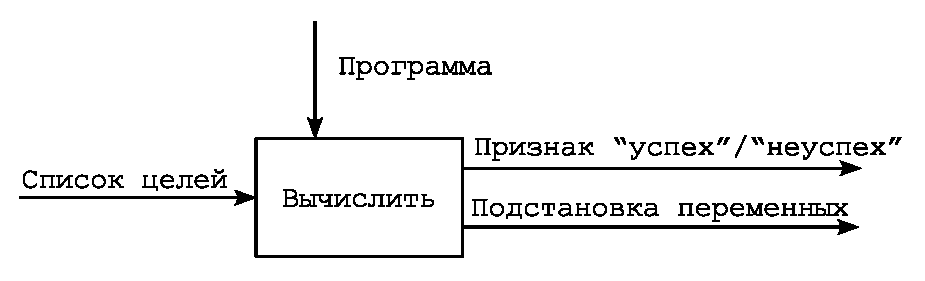
\includegraphics[scale=0.7]{pics/imp_proc.eps}
\end{center}
\caption{Входы и выходы процедуры вычисления списка целей.}
\label{pic:proc}
\end{figure}

\noindent Смысл двух составляющих выхода такой:
\begin{itemize}
\item[(1)] Признак <<успех>>/<<неуспех>> принимает значение {\tt да}, если цели достижимы, и {\tt нет} --- в противном случае. Будем говорить, что {\tt да} сигнализирует об {\bf успешном} завершении, и {\tt нет} --- о {\bf неуспехе}.

\item[(2)] Подстановка переменных порождается процедурой только в случае успешного завершения; в случае неуспеха подстановка отсутствует.
\end{itemize}

\begin{example}\label{ex:bear}
Пример, иллюстрирующий процедурную семантику Пролога: последовательность вычислений, выполняемых процедурой {\tt вычислить}.
\end{example}\label{ex:interp}
\paragraph{ПРОГРАММА.} Пусть дана следующая программа.
{\tt\begin{verbatim}
    big(bear).      % Предложение 1
    big(elephant).  % Предложение 2
    big(cat).       % Предложение 3
    brown(bear).    % Предложение 4
    black(cat).     % Предложение 5
    gray(elephant). % Предложение 6
    dark(Z) :-      % Предложение 7:
        black(Z).   % Любой черный объект
                    %   является темным
    dark(Z) :-      % Предложение 8:
        brown(Z).   % Любой коричневый объект
                    %   является темным
\end{verbatim}}

\paragraph{ЗАПРОС.} Зададим следующий запрос.
{\tt\begin{verbatim}
| ?- dark(X), big(X).
        % Кто одновременно темный и большой?
\end{verbatim}}

\paragraph{Шаги вычислений.}
\begin{itemize}
\item[(1)] Исходный список целевых утверждений:
{\tt\begin{verbatim}
    dark(X), big(X).
\end{verbatim}}

\item[(2)] Просмотр всей программы от начала к концу и поиск предложения, у которого голова сопоставима с первым целевым утверждением
{\tt\begin{verbatim}
    dark(X).
\end{verbatim}}

\noindent Найдена формула 7:

{\tt\begin{verbatim}
    dark(Z) :- black(Z).
\end{verbatim}}

\noindent Замена первого целевого утверждения конкретизированным телом предложения 7 - порождение нового списка целевых утверждений.

{\tt\begin{verbatim}
    black(X), big(X).
\end{verbatim}}

\item[(3)] Просмотр программы для нахождения предложения, сопоставимого с \texttt{black(X)}. Найдено предложение 5: \texttt{black(cat)}. У этого предложения нет тела, поэтому список целей при соответствующей конкретизации сокращается до
{\tt\begin{verbatim}
    big(cat).
\end{verbatim}}

\item[(4)] Просмотр программы в поисках цели \texttt{big(cat).} Ни одно предложение не найдено. Поэтому происходит возврат к шагу (3) и отмена конкретизации {\tt X~=~cat}.
Список целей теперь снова
{\tt\begin{verbatim}
    black(X), big(X)
\end{verbatim}}

\noindent Продолжение просмотра программы ниже предложения 5. Ни одно предложение не найдено. Поэтому возврат к шагу (2) и продолжение просмотра ниже предложения 7. Найдено предложение 8:
{\tt\begin{verbatim}
    dark(Z) :- brown(Z).
\end{verbatim}}
\noindent   Замена первой цели в списке на \texttt{brown(Х)}, что дает
{\tt\begin{verbatim}
    brown(X), big(X)
\end{verbatim}}

\item[(5)] Просмотр программы для обнаружения предложения, сопоставимого \texttt{brown(X)}. Найдено предложение \texttt{brown(bear)}. У этого предложения нет тела, поэтому список целей уменьшается до
{\tt\begin{verbatim}
    big(bear).
\end{verbatim}}

\item[(6)] Просмотр программы и обнаружение факта \texttt{big(bear)}. У него нет тела, поэтому список целей становится пустым. Это указывает на успешное завершение.
\end{itemize}

В оставшейся части данного раздела приводится несколько более формальное и систематическое описание приведенного процесса. Конкретные операции, выполняемые в процессе вычисления целевых утверждений, показаны в приведенном примере \ref{ex:bear}. Возможно, следует изучить этот рисунок прежде, чем знакомиться с последующим общим описанием.

Чтобы вычислить список целевых утверждений
$$
    G_1, G_2, \ldots, G_m,
$$
процедура \textbf{вычислить} делает следующее:
\begin{itemize}
  \item Если список целей пуст - завершает работу \textbf{успешно}.
  \item Если список целей не пуст, продолжает работу, выполняя (описанную далее) операцию {\tt просмотр}.
  \item Операция \texttt{просмотр}: Просматривает предложения программы от начала к концу до обнаружения первого предложения $C$, такого, что голова $C$ сопоставима с первой целью $G_1$. Если такого предложения обнаружить не удается, то работа заканчивается \textbf{неуспехом}.

\noindent Если $C$ найдено и имеет вид\\[1ex]
\verb|    |$H$ {\tt :-} $B_1${\tt,} \ldots{\tt,} $B_n${\tt,}

\noindent то переменные в $C$ переименовываются, чтобы получить такой вариант $C'$ предложения $C$, в котором нет общих переменных со списком $G_1, \ldots, G_m$. Пусть $C'$ --- это\\[1ex]
\verb|    |$H'$ {\tt :-} $B'_1${\tt,} \ldots{\tt,} $B'_n${\tt.}

\noindent Сопоставляется $G_1$ с $H'$; пусть $S$ --- результирующая конкретизация переменных. В списке целей $G_1$, $G_2$, \ldots, $G_m$, цель $G_1$ заменяется на список $B_1'${\tt,} \ldots{\tt,} $B'_n$, что порождает новый список
целей:\\[1ex]
\verb|    |$B_1'${\tt ,} \ldots{\tt,} $B_n'${\tt,} $G_2${\tt,}
    \ldots{\tt,} $G_m${\tt.}

\noindent Заметим, если $C$ --- факт, тогда $n = 0$, и в этом случае
новый список целей оказывается короче, нежели исходный; такое уменьшение списка целей может в определенных случаях превратить его в пустой, а следовательно, --- привести к успешному завершению.

\noindent Переменные в новом списке целей заменяются новыми значениями, как
это предписывает конкретизация $S$, что порождает еще один список целей\\[1ex]
\verb|    |$B_1>>${\tt ,} \ldots{\tt,} $B_n>>${\tt,} $G_2${\tt,}
    \ldots{\tt,} $G_m${\tt.}

  \item Вычисляет (используя рекурсивно ту же самую процедуру) этот новый список целей. Если его вычисление завершается успешно, то и вычисление исходного списка целей тоже завершается успешно. Если же его вычисление порождает неуспех, тогда новый список целей отбрасывается и происходит возврат (backtrack) к просмотру программы. Этот просмотр продолжается, начиная с предложения, непосредственно следующего за предложением $C$ ($C$ --- предложение, использовавшееся последним), и делается попытка достичь успешного завершения с помощью другого предложения.
\end{itemize}

\subsection{Примеры интерпретаций программ}
Для того чтобы продемонстрировать <<полярность>> декларативной и процедурной интерпретации (семантики), рассмотрим еще два примера:

\begin{example}
Определить декларативную и процедурную семантику (смысл) следующего предложения языка Пролог.
\end{example}
{\tt\begin{verbatim}
    P :- P.
\end{verbatim}}

\paragraph{Декларативная интерпретация.}
\noindent Семантика (смысл) предложения выражается фразой: <<{\tt P} истинно, если истинно {\tt P}>>. С декларативной точки зрения фраза совершенно корректна\footnote{Нетрудно доказать ее истинность при любых истинностных значениях {\tt P}, например при помощи метода <<от противного>>.} (эта фраза --- тавтология),  однако в процедурном смысле это предложение бесполезно. Более того, для Пролог-системы такое предложение может породить серьезную проблему. Рассмотрим запрос к этой программе:
{\tt\begin{verbatim}
| ?- P.
\end{verbatim}}
\noindent При использовании вышеприведенного предложения {\tt P} будет заменено на ту же самую цель {\tt P}, она, в свою очередь, будет заменена снова на {\tt P} и т.~д. В этом случае система войдет в бесконечный цикл, не замечая, что никакого продвижения в вычислениях не происходит.

Рассмотрим другой пример.
\begin{example}
Определить декларативную и процедурную семантику следующего предложения языка Пролог.
\end{example}
{\tt\begin{verbatim}
    P.
    P :- P.
\end{verbatim}}

\noindent С точки зрения декларативного смысла добавление {\tt P} как факта излишне, как излишне было бы добавление {\tt P~:-~P} к факту {\tt P}. В обоих случаях мы имеем дело с {\bf истинными}\footnote{Факт {\tt P} истинен по определению, а {\tt P~:-~P} истинно, так как это тавтология (теорема).} высказываниями. Однако с процедурной точки зрения программа представляет интерес. Пусть в Пролог-систему введен запрос:
{\tt\begin{verbatim}
    P.
\end{verbatim}}
\noindent Цель {\tt P} сопоставляется с фактом {\tt P}, и при этом получается пустое множество --- выполнение завершается {\bf удачно}. Если {\tt P} --- это часть тела какого-либо правила $C$, то в процессе доказательства $C$ возможны возвраты, в том чмсле и к {\tt P}. В этом случае сопоставление цели (подцели правила $C$) {\tt P} с фактом {\tt P} {\bf отменяется} и производится замена цели {\tt P} по правилу {\tt P~:-~P} на <<новую>> цель {\tt P}. Далее, для этой цели выполняются вычисления, начиная с сопоставления ее с фактом {\tt P}. Всякий раз, отменяя предыдущее сопоставление цели {\tt P} с фактом {\tt P}, Пролог порождает новую (как правило, такую же) ветвь поиска сопоставлений для подцелей в $C$, стоящих {\bf за} подцелью {\tt P}. Таким образом, возврат (backtrtack) из $C$ никогда не может быть сделан\footnote{За исключением случая, если в теле $C$ есть предикат <<отсечение>> (<<{\tt !}>>), и этот предикат будет достигнут.}.

Описанный предикат {\tt P} находит свое применение в подпрограммах пользовательских интерфейсов как способ организации бесконечного цикла (см. указания к лабораторной работе 3). Более того, он имеет собственное имя:
{\tt\begin{verbatim}
    Repeat.
    Repeat :- Repeat.
\end{verbatim}}

\begin{questions}
  \item{} Дайте определение декларативной интерпретации Пролог-про\-грамм.
  \item{} Дайте определение процедурной интерпретации Пролог-про\-грамм.
  \item{} Как можно использовать предикат \texttt{repeat}?
  \item{} Какова процедурная интерпретация следующего высказывания языка Пролог: \texttt{A :- Q,W,E;R,T,Y.}?
\end{questions}


\chapter{Управление логическим выводом}
Прежде всего программист может управлять процессом вычислений по программе, располагая ее предложения и цели в том или ином порядке \cite{Bratko}. В данной главе мы рассмотрим еще одно средство управления, получившее название {\em отсечение} (cut) и предназначенное для ограничения автоматического перебора.

\section{Ограничение перебора}
В процессе достижения цели Пролог-система осуществляет автоматический перебор вариантов, делая возврат при неуспехе како\-го-либо из них. Такой перебор --- полезный программный механизм, поскольку он освобождает пользователя от необходимости программировать его самому. С другой стороны, ничем не ограниченный перебор может стать источником {\bf неэффективности} программы. Поэтому иногда требуется его ограничить или исключить вовсе. Для этого в Прологе предусмотрена конструкция <<отсечение>>.

Давайте сначала рассмотрим простую программу, процесс вычислений в которой содержит ненужный перебор. Мы выделим те точки этого процесса, где перебор бесполезен и ведет к неэффективности.

Рассмотрим двухступенчатую функцию на рис.~\ref{pic:func_step}. Связь между $X$ и $Y$ можно определить с помощью следующих трех правил:

\emph{Правило 1:} если $X < 3$, то $Y = 0$.

\emph{Правило 2:} если $3 \leq X < 6$, то $Y = 2$.

\emph{Правило 3:} если $6 \leq X$, то $Y = 4$.

\begin{figure}[ht]
\begin{center}
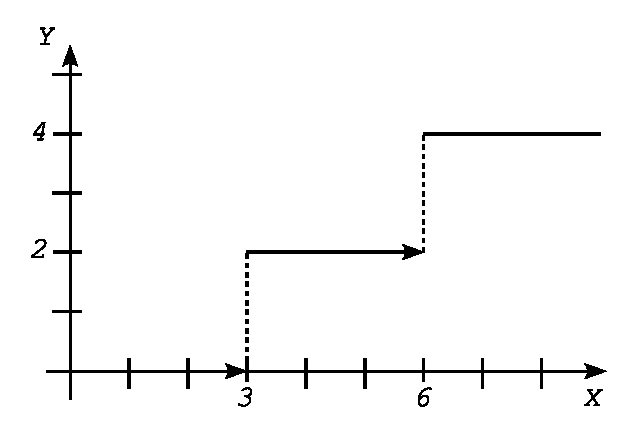
\includegraphics[scale=0.7]{pics/func_step.eps}
\end{center}
\caption{Двухступенчатая функция} \label{pic:func_step}
\end{figure}

\noindent На Прологе это можно выразить с помощью бинарного отношения
\texttt{f(X, Y)} так:
{\tt \begin{verbatim}
    f(X, 0) :- X < 3.          % Правило 1
    f(X, 2) :- 3 =< X, X < 6.  % Правило 2
    f(X, 4) :- 6 =< X.         % Правило 3
\end{verbatim}}

В этой программе предполагается, конечно, что к моменту начала вычисления {\tt f(X, Y)} {\tt X} уже конкретизирован каким-либо числом; это необходимо для выполнения операторов сравнения.

Мы проделаем с этой программой два эксперимента. Каждый из них обнаружит в ней свой источник неэффективности, и мы устраним оба этих источника по очереди, применив оператор отсечения.

\paragraph{Эксперимент 1.} Проанализируем, что произойдет, если задать следующий запрос:
{\tt \begin{verbatim}
| ?- f(1, Y), 2 < Y.
\end{verbatim}}

При вычислении первой цели {\tt f(1,Y)} {\tt Y} конкретизируется нулем. Поэтому вторая цель становится такой:
{\tt \begin{verbatim}
    2 < 0.
\end{verbatim}}
\noindent Она терпит неудачу, и поэтому и весь список целей также терпит неудачу. Это очевидно, однако перед тем, как признать, что такому списку целей удовлетворить нельзя, Пролог-система при помощи возвратов попытается проверить еще две бесполезные в данном случае альтернативы.

Три правила, входящие в отношение {\tt f}, являются взаимоисключающими, поэтому успех возможен, самое б\'{о}льшее, в одном из них. Следовательно, мы (но не Пролог-система) знаем, что как только успех наступил в одном из них, нет смысла проверять остальные, поскольку они все равно обречены на неудачу. Для предотвращения бессмысленного перебора мы должны явно указать Пролог-системе, что {\bf не нужно} осуществлять возврат из этой точки. Мы можем сделать это при помощи конструкции отсечения. Отсечение записывается в виде символа <<{\tt !}>>, который вставляется между целями и играет роль некоторой псевдоцели. Вот наша программа, переписанная с использованием отсечения:

{\tt \begin{verbatim}
    f(X, 0) :- X < 3, !.
    f(X, 2) :- 3 =< X, X < 6, !.
    f(X, 4) :- 6 =< X.
\end{verbatim}}

Символ <<{\tt !}>> предотвращает возврат из тех точек программы, в которых он поставлен. Зададим вопрос:
{\tt \begin{verbatim}
| ?- f(1, Y), 2 < Y.
\end{verbatim}}
\noindent Пролог-система породит ветвь дерева. Эта ветвь потерпит неудачу на цели {\tt 2~<~0}. Система попытается сделать возврат, но вернуться она сможет не далее точки, помеченной в программе символом <<{\tt !}>>. Альтернативные ветви, соответствующие правилу 2 и правилу 3, порождены не будут.

Новая программа, снабженная отcечениями, во всех случаях более эффективна, чем первая версия, в которой они отсутствуют. Неудачные варианты новая программа распознает всегда быстрее, чем старая.

Вывод: добавив отсечения, мы повысили эффективность. Если их теперь убрать, программа породит тот же результат, только на его получение она потратит, скорее всего, больше времени. Можно сказать, что в нашем случае после введения отсечений мы {\bf изменили только процедурную семантику} программы, оставив при этом ее декларативную семантику в неприкосновенности. В дальнейшем мы покажем, что использование отсечения может также затронуть и {\bf декларативную семантику} программы.

\paragraph{Эксперимент 2.} Проделаем теперь еще один эксперимент со второй версией нашей программы. Предположим, мы задаем вопрос:
{\tt \begin{verbatim}
| ?- f(7, Y), Y = 4.
\end{verbatim}}
\noindent Проанализируем, что произошло. Перед тем, как был получен ответ, система пробовала применить все три правила. Эти попытки породили следующую последовательность целей:

\noindent{}\emph{попытка применить правило 1:}
$7 < 3$ терпит неудачу, происходит возврат и попытка применить правило 2 (точка отсечения достигнута не была);

\noindent{}\emph{попытка применить правило 2:} $3\leq 7$ <<успех>>, но $7 < 6$ терпит неудачу; возврат и попытка применить правило 3 (точка отсечения снова не достигнута);

\noindent{}\emph{попытка применить правило 3:} {$6\leq 7$} --- <<успех>>.

Приведенные этапы вычисления обнаруживают еще один источник неэффективности. Вначале выясняется, что {\tt X < 3} не является истиной ($7 < 3$ терпит неудачу). Следующая цель --- {\tt 3~=<~X} ($3 \leq 7$ ---  <<успех>>). Но нам известно, что если первая проверка неуспешна, то вторая обязательно будет успешной, так как второе --- целевое утверждение является отрицанием первого. Следовательно, {\bf вторая проверка лишняя} и соответствующую цель можно опустить. То же самое верно и для цели {\tt 6~=<~X} в правиле 3. Все эти соображения приводят к следующей, более экономной формулировке наших трех правил:

если $X < 3$, то $Y = 0$;

иначе, если $X < 6$, то $Y = 2$;

иначе $Y = 4$.

Теперь мы можем опустить в нашей программе те условия, которые обязательно выполняются при любом вычислении. Получается третья версия программы:
{\tt \begin{verbatim}
    f(X, 0) :- X < 3, !.
    f(X, 2) :- X < 6, !.
    f(X, 4).
\end{verbatim}}

\noindent Эта программа дает тот же результат, что и исходная, но более эффективна, чем обе предыдущие. Однако что будет, если мы теперь удалим отсечения? Программа станет такой:
{\tt \begin{verbatim}
    f(X, 0) :- X < 3.
    f(X, 2) :- X < 6.
    f(X, 4).
\end{verbatim}}
\noindent Она может порождать различные решения, часть из которых неверны. Например:

{\tt \begin{verbatim}
| ?- f( 1, Y).
     Y = 0,
     Y = 2,
     Y = 4.
 \end{verbatim}}

Важно заметить, что в последней версии, в отличие от предыдущей, отсечения затрагивают не только процедурное поведение, но {\bf изменяют} также и {\bf декларативную семантику} программы.

Более точный смысл механизма отсечений можно сформулировать следующим образом:
\begin{quote}
Назовем <<целью-родителем>> ту цель, которая сопоставилась с головой предложения, содержащего отсечение. Когда в качестве цели встречается отсечение, такая цель сразу же считается успешной и при этом заставляет систему принять те альтернативы, которые были выбраны с момента активизации цели-родителя до момента, когда встретилось отсечение. Все оставшиеся в этом промежутке (от цели-родителя до отсечения) альтернативы не рассматриваются.
\end{quote}

Чтобы прояснить смысл этого определения, рассмотрим предложение вида\\[1ex]
\verb|    |$H$ {\tt :-} $B_1${\tt,} $B_2${\tt,} \ldots {\tt ,} $B_m${\tt,}
    {\tt !,} \ldots {\tt ,} $B_n${\tt.}\\[-0.5ex]

\noindent Будем считать, что это предложение активизировалось, когда некоторая цель $G$ сопоставилась с $H$. Тогда $G$ является целью-родителем. В момент, когда встретилось отсечение, успех уже наступил в целях $B_1$, \ldots, $B_m$. При выполнении отсечения это (текущее) решение $B_1$, \ldots, $B_m$ {\bf замораживается} и все возможные оставшиеся альтернативы больше не рассматриваются. Далее, цель $G$ связывается теперь с этим предложением: любая попытка сопоставить $G$ с головой какого-либо другого предложения пресекается.

Применим эти правила к следующему примеру:
{\tt \begin{verbatim}
    С :- Р, Q, R, !, S, Т, U.
    С :- V.
    А :- В, С, D.

| ?- А.
\end{verbatim}}

Здесь {\tt А}, {\tt В}, {\tt С}, {\tt D}, {\tt P} и т.~д. имеют синтаксис предикатов. Отсечение повлияет на вычисление цели {\tt С} следующим образом. Перебор будет возможен в списке целей {\tt Р}, {\tt Q}, {\tt R}; однако как только точка отсечения будет достигнута, все альтернативные решения для этого списка изымаются из рассмотрения. Альтернативное предложение, входящее в {\tt С}:
{\tt \begin{verbatim}
    С :- V.
\end{verbatim}}
\noindent также не будет учитываться. Тем не менее, перебор будет возможен в списке целей {\tt S}, {\tt T}, {\tt U}. Цель-родитель предложения, содержащего отсечения, --- это цель $C$ в предложении
{\tt \begin{verbatim}
    А :- В, С, D.
\end{verbatim}}

Поэтому отсечение повлияет только на цель {\tt С}. С другой стороны, оно будет невидимо из цели {\tt А}. Таким образом, автоматический перебор все равно будет происходить в списке целей {\tt В}, {\tt С}, {\tt D}, вне зависимости от наличия отсечения в предложении, которое используется для достижения {\tt С}.

\subsection{Примеры, использующие отсечение}
\paragraph{Вычисление максимума.}
Процедуру нахождения наибольшего из двух чисел можно запрограммировать в виде отношения {\tt max(X, Y, М)}, где {\tt М = X}, если {\tt X} больше или равен {\tt Y}, и {\tt М} есть {\tt Y}, если {\tt X} меньше {\tt Y}. Это соответствует двум таким предложениям:

{\tt \begin{verbatim}
    max(X, Y, X) :- X >= Y.
    max(X, Y, Y) :- X < Y.
\end{verbatim}}

Эти правила являются взаимно исключающими. Если выполняется первое, второе обязательно потерпит неудачу. Если неудачу терпит первое, второе обязательно должно выполниться. Поэтому возможна более экономная формулировка, использующая понятие иначе:

если $X \geq Y$, то $M = X$,

иначе $M = Y$.

На Прологе это записывается при помощи отсечения:
{\tt \begin{verbatim}
    max( X, Y, X) :- X >= Y, !.
    max( X, Y, Y).
\end{verbatim}}

\paragraph{Проверка принадлежности списку, порождающая един\-ствен\-ное
решение.} Для того чтобы узнать, принадлежит ли {\tt X} списку {\tt L}, мы пользовались отношением {\tt in/2}, и программа была следующей:
{\tt \begin{verbatim}
    in(R, [R | Т]).
    in(R, [H | Т]) :- in(R, T).
\end{verbatim}}

\noindent Эта программа дает <<недетерминированный>> ответ: если {\tt R} встречается в списке несколько раз, то будет найдено {\bf каждое} его вхождение. Следующая программа исправляет этот <<недостаток>> и выдает только одно решение.
{\tt \begin{verbatim}
    in(R, [R | Т]) :- !.
    in(R, [H | Т]) :- in(R, T).
\end{verbatim}}

\subsection{Другие предикаты управления выводом}

В языке программирования Пролог существуют еще несколько предикатов и логическая связка, используемые для управления процессом вывода.

\begin{description}
\item[{\tt $\backslash$+}] Логическая операция отрицания <<$\neg$>> имеет, с одной стороны, противоположное истинностное значение истинностному значению пре\-ди\-ка\-та, который следует за этой операцией, с другой стороны, {\tt \verb|\+| G} ложен, если Пролог для  {\tt G} смог построить вывод.
\item[\tt fail/0] Этот предикат обозначает <<ложь>>, т.~е. если он включен как подцель тела правила или запроса, то это правило и запрос никогда не будут доказаны. Предикат используется для организации перебора всех решений в части программы, где задана цель \texttt{init/0}, например, программа
{\tt \begin{verbatim}
    number(1). number(2). number(3).
    number(4). number(5). number(6).

    init:-
        number(X), number(Y), write(X),
        write(Y), fail.
:- initialization(init).
\end{verbatim}}
выведет на экран все двузначные комбинации цифр от 1 до 6. Если убрать {\tt fail} из запроса, то будет выведена только одна комбинация.
\item[\tt nonvar/1] В ISO-Prolog предикат {\tt nonvar/1} истинный, если пе\-ре\-мен\-ная-аргумент к этому моменту уже приобрела свое значение, и ложный --- в обратном случае.
\item[\tt var/1] Предикат {\tt var/1} истинный тогда и только тогда, когда предикат {\tt nonvar/1} ложный.
\end{description}

\begin{example}  Пусть дано уравнение
$$
    y=k\cdot x,
$$
причем комбинации значений переменных и их отсутствия могут быть любыми. Предложить программу, определяющую значения переменных, которые неизвестны,  либо выдать на экран соответствующее сообщение. Равенство должно сохраняться.
\end{example}

Решение задачи (программа) будет строиться для каждого набора переменных, всего их $2^3=8$\footnote{Надо учесть также комбинации нулевых значений.}, но некоторые могут быть объединены.

{\tt \begin{verbatim}
    solve(Y, K, X) :-
        nonvar(K), nonvar(X), !,
            % Y может быть как связанным, так и
            % свободным.
        Y is K * X.
    solve(Y, K, X) :-
        nonvar(Y), nonvar(X),
        X <> 0,
        K is Y / X.
    solve(Y, K, X) :-
        nonvar(Y), nonvar(X),
        X = 0,
        write('Нет решений'), nl.
    solve(Y, K, X) :-
        nonvar(Y), nonvar(K),
            % сократим себе программу!
        solve(Y, X, K).
    solve(Y, K, X) :-
        var(X), var(K), nonvar(X)
        write('Множество решений'), nl,
        format('X = Y / ~w', [K]), nl.
    ........% и т.~д.
\end{verbatim}}


\section{Лабораторная работа 2: Списки}

\paragraph{Задание.} В pаботе тpебуется реализовать {\bf по крайней мере два отношения} из индивидуального задания в виде правил и фактов на языке Пpолог. К программе требуется выполнить ряд запросов, объяснить выдаваемые системой результаты: дать процедурную и декларативную интерпретацию определенных отношений.

\paragraph{Цель работы.} Приобрести навыки рекурсивной обработки рекурсивных структур данных; научиться интерпретировать (переводить на естественный язык) Пролог-программы.

\paragraph{Время работы.} На выполнение работы отводится два академических часа.

\paragraph{Индивидуальные задания}
\begin{enumerate}
\item Сформировать новый список из всех четных элементов списка.
\item Опpеделить, является ли один список подсписком дpугого.
\item Удалить все вхождения заданного элемента из списка.
\item Hаписать пpогpамму пословного (подстрочного) пеpевода пpедложения, представленного в виде списка слов, с английского на фpанцузский (или любой другой) язык.
\item Сфоpмиpовать новый список, в котоpом каждый элемент исходного списка входит в новый список два pаза подряд.
\item Слить два упоpядоченных списка, сохpанив упоpядоченность.
\item Опpеделить, являются ли два заданных элемента соседними в списке.
\item Опpеделить последний элемент списка.
\item Подсчитать количество элементов списка.
\item Упорядочить список методом пузырька.
\item Упорядочить список методом вставки.
\item Упорядочить список методом быстрой сортировки.
\item Заменить элемент списка на заданное значение.
\item Определить все перестановки элементов списка.
\item Найти сумму элементов списка, стоящих  на нечетных  местах в  списке.
\item Инвертировать список (составить элементы в обратном порядке).
\item Добавить элемент в конец списка.
\item Удалить два последних элемента списка.
\item Найти максимальный элемент списка.
\item В заданном списке выделить подсписок, содержащий $N$ элементов с начала списка.
\item В заданном  списке выделить подсписок, начиная с $N$-го элемента списка и кончая $K$-м элементом этого же списка.
\item Определить сумму отрицательных элементов списка, стоящих на четных местах.
\item Удалить из списка максимальный элемент.
\item Выполнить циклический сдвиг списка на заданное число элементов. Например, результат сдвига списка {\tt [a, b, c, d]} на два элемента есть список {\tt [c, d, a, b]}.
\item Определить предикат {\tt code(Х, List)}, где {\tt Х} --- целое неотрицательное число {\tt (0}$\leq${\tt X}$\leq${\tt 9)}, а {\tt List} --- это последовательность  единичек, число  которых  равно  {\tt Х}.  Например, {\tt code(3, L)} дает {\tt L=[1, 1, 1]}, а {\tt code(0, L)} дает {\tt L=[]}.
\item Определить двуаргументный предикат {\tt translate(С1, С2)} для перевода списка цифр в список соответствующих слов. Например, истинным будет следующее высказывание\\
     {\tt translate([3, 4, 8], ['три', 'четыре', 'восемь'])}.
\end{enumerate}

\subsubsection*{Методические указания к выполнению лабораторной работы}
  Сначала необходимо понять, между какими объектами задается отношение, его арность (все то же самое, как и в предыдущей лабораторной работе). Далее:
  \begin{enumerate}
  \item Сначала определить частный случай (самый простой) отношения (в терминах доказательства теорем методом математической индукции {\tt P(0, \ldots)} --- база индукции).
  \item Затем в предположении, что условие базы индукции ложно, определить для всех остальных случаев {\tt P(n, \ldots)$\to$P(n+1, \ldots)}.
  \end{enumerate}

\begin{example}
  Задача --- определить последний элемент списка.
\end{example}
  Отношение задается между списками и элементами списка. Арность отношения --- 2.

Частный случай --- одноэлементный список (пустой список не имеет последнего элемента). Предикат интерпретируется следующим образом: <<Последний элемент одноэлементного списка и есть этот единственный элемент>>.

{\tt\begin{verbatim}
    last([X], X).
\end{verbatim}}

Пусть список содержит не меньше одного элемента (отрицание предыдущего утверждения), тогда последний элемент списка --- это последний элемент его хвоста.

{\tt\begin{verbatim}
    last([_ | T], X) :- last(T, X).
\end{verbatim}}
\emph{Декларативная интерпретация}: Последний элемент одноэлементного списка и есть требуемый элемент (решение). Если список содержит более одного элемента, то последний элемент этого списка --- последний элемент хвоста.

\emph{Процедурная интерпретация}: Чтобы найти последний элемент списка, нужно: если список содержит лишь один элемент, то предъявить в качестве второго элемента отношения (результата) {\tt last/2} первый элемент списка. Иначе, если в списке содержится более одного элемента, то: (a)~найти последний элемент хвоста и (б) предъявить его как результат.

\begin{questions}
\item{} Что является причиной неэффективности системы программирования Пролог?
\item{} Какова семантика предиката <<отсечение>>?
\item{} Каково будет истинностное значение запроса \texttt{| ?- var(X).}?
\item{} Какова процедурная интерпретация правила \texttt{A :- Q,W,E,!, R,T,Y.}?
\item{} Возымеет ли действие отсечение в запросе \texttt{fail,!.}?
\end{questions}

\chapter{Предикаты с побочными действиями}
Пролог обладает возможностью не только определять условия, когда значения предикатов истинны, но и выполнять некоторую <<полезную>> работу, такую как получать значение с клавиатуры, выводить сообщения на экран, складывать и вычитать и т.~д. Предикаты, выполняющие эти действия, делятся на два класса: {\em арифметические} и так называемые {\em предикаты с побочными действиями}.

Для выполнения арифметических операций используется предикат <<{\tt is/2}>>.
\begin{example}
Решение квадратного уравнения <<по-прологовски>>. Пусть даны $a$, $b$, $c$ такие, что
$$
    ax^2+bx+c=0.
$$
Найти такие значения $x$, чтобы равенство сохранялось\footnote{Предполагаем, что {\tt A, B, C} заданы (конкретизированы).}.
\end{example}
{\tt\begin{verbatim}
    sqeq(A, B, C, X) :-
        D is B * B + 4 * A * C,
        sd(A, B, C, D, X).
    sd(A, B, C, D, X) :-
        D < 0,
        write('Решения в области'), nl,
        write('комплексных чисел.'), nl,
        !, fail.
    sd(A, B, C, D, X) :-
        D = 0,
        write('Четные корни'), nl,
        X is - (B * B) / (2 * A).
    sd(A, B, C, D, X) :-
        D > 0,
        X is ( - (B * B) + sqrt(D) ) / (2 * A).
    sd(A, B, C, D, X) :-
        D > 0,
        X is ( - (B * B) - sqrt(D) ) / (2 * A).
\end{verbatim}}

Кроме арифметических операций в программе использованы предикаты с побочными действиями {\tt write/1} и {\tt nl/0}. Кроме этих необходимо выделить следующие предикаты для ввода данных в GNU-Prolog:
\begin{description}
\item[\tt read\_token/1] вводит с клавиатуры лексическую единицу до нажатия клавиши <<Enter>>. Вариант лексической единицы выдается в виде атома. Например, если пользователь с клавиатуры вводит <<10>>, то переменная аргумента конкретизируется атомом <<10>>, если пользователь вводит <<F>>, то аргумент конкретизируется атомом <<\texttt{var(`F`)}>>.
\item[\tt read\_term/1] или просто \texttt{read/1} вводит с клавиатуры терм: пользователь должен ввести синтаксически правильную конструкцию, заканчивающуюся точкой <<\texttt{.}>>. Пример:
{\tt\begin{verbatim}
| ?- read(A).
a(s),b(k).    % Вводит пользователь.

A = (a(s),b(k))

yes.
\end{verbatim}}
\end{description}

Для отображения результатов вывода удобно использовать предикат \texttt{format/2}. Предикат выполняет аналогичную функцию формирования сообщения из индивидуальных составляющих и вывода на экран (или в файл), что и функция \texttt{printf}. Спецификация предиката --- \texttt{format(Format, Arguments)}, где \texttt{Format} --- это форматная строка, \texttt{Arguments} --- список аргументов, которые будут подставлены в форматную строку. Например, следующий запрос
{\tt\begin{verbatim}
| ?- A=8, B=c(Y), E='test',
    format('A=~w, B=~w, E=~w ~n !!! ',
       [A,B,E]).
A=8, B=c(_22), E=test
 !!!

A = 8
B = c(Y)
E = test

yes.
\end{verbatim}}
\noindent{}Здесь, \verb|~w| обозначает печать аргумента при помощи средств предиката \texttt{write/1}, \verb|~n| --- перевод строки. В этом примере терм \texttt{B=c(Y)} распечатался как \texttt{B=C\_22}: машине вывода Пролога все равно, как называются переменные, которые вводятся процедурой поиска логического вывода Пролог, имена порождаются последовательным перебором чисел.

\rem{Кроме того, существуют\footnote{Список встроенных предикатов GNU-Prolog можно найти в документации.} также предикаты управления базой данных пролога (см. следующий раздел), предикаты управления вводом-выводом, предикаты трассировки выполнения программы и т.~п.}

\section{Базы данных в Прологе}

Очень коротко рассмотрим возможности Пролога вести базу данных. {\em Базой данных} Пролога называется {\bf изменяемый} набор фактов (а также правил)\footnote{Вы уже знакомы с предикатами {\tt consult/1} и {\tt reconsult}.}. Чтобы набор фактов был изменяемым, надо его таковым объявить:
{\tt\begin{verbatim}
        % группа: обозначение, название
:- dynamic(group/2).
        % студент: номер зачетки, группа, Ф.~И.~О.
:- dynamic(student/3).
\end{verbatim}}

\noindent Как нетрудно догадаться, запросы к базе данных в Прологе делаются так же, как и к другим правилам и фактам (предполагается, что база данных Прологу известна):
{\tt\begin{verbatim}
     % в какой группе учится студент
     % Иванов Иван
| ?- group(X),
     student(_, X, 'Иванов Иван').
     X = '02421',
     % Выдать всех студентов указанной группы
| ?- group(X, '02421'),
         student(_, X, Y).
     X = '02421', Y = 'Иванов Иван';
     . . . . .
 \end{verbatim}}

Добавлять и удалять факты в базе данных можно с помощью предикатов с побочными действиями {\tt assert/1} и {\tt retract/1}:

{\tt\begin{verbatim}
    add_student(Group, Num, Name) :-
        assert(student(Num, Group, Name)).
\end{verbatim}}

\noindent Замечание: все аргументы предиката {\tt assert/1} должны быть {\bf конкретизированными} переменными.

{\tt\begin{verbatim}
    del_student(Group, Num, Name) :-
        retract(student(Num, Group, Name)).
\end{verbatim}}
\noindent Предыдущее замечание не имеет силы для {\tt retract/1}, однако он будет истинным, если удалит первый попавшийся факт, удовлетворяющий ограничениям, указанным значениями переменных.

Существуют разновидности предиката добавления факта в базу данных: {\tt asserta/1} и {\tt assertz/1}, которые добавляют факты, соответственно, в начало или конец существующего списка фактов.

Базу данных можно загрузить из текстового файла при помощи предиката {\tt consult/1}, причем выполнить его надо после объявления предиката динамическим.

\section{Лабораторная работа 3: Базы данных}
\paragraph{Задание.} Необходимо разработать {\bf интерактивную} программу ведения базы данных. База данных должна содержать {\bf по крайней мере одно} отношение <<один-ко-многим>> ($1$:$N$) или <<многие-ко-многим>> ($N$:$M$). Кроме того, необходимо реализовать выполнение {\bf запроса}, демонстрирующего эту связь, а также корректно реализовать функцию удаления записей.

\paragraph{Цель работы.} Ознакомиться с вариантом реализации принципа реляционных баз данных в виде Пролог-программы. Научиться пользоваться предикатами с побочными действиями, а также управлять процессом поиска решения Пролог-системой.

\paragraph{Время работы.} На выполнение работы отводится четыре академических часа.

\subsubsection*{Методические указания к выполнению лабораторной работы.} Для непривычного к логическому программированию ума программиста довольно трудно реализовать меню на Прологе, однако, это сделать легче, чем в каком-либо другом языке программирования. Внимательно разберите следующий пример:

{\tt\begin{verbatim}
    menu_do(1) :-
        write('Приступим к добавлению записи...'),
        .......
    menu_do(0).

    main :-
        repeat,
        write('Меню программы:'), nl,
        write('1 - добавление ...), nl,
        .....
        write('0 - выход из программы'), nl,
        write(' > '), read_int(I),
        menu_do(I),
        I = 0, !.
\end{verbatim}}

\paragraph{Индивидуальные задания.}
Разработайте на Прологе программу управления базой данных в следующих предметных областях\footnote{Взято с \url{http://crec.mipt.ru/study/materials/db/DBvariants.doc}.}:
\begin{enumerate}
\item Институт (деканаты, кафедры, учебный отдел).
\begin{itemize}
\item Студенты: паспортные данные, адрес, дата зачисления, номер приказа, факультет, группа, является ли старостой, кафедра (специализация), изучаемые (изученные) предметы, оценки, задолженности, стипендия.
\item Учебные курсы: название, факультет(ы), групп(ы), кафедра, семестр(ы), форма отчетности, число часов.
\item Преподаватели: паспортные данные, адрес, телефон, фотография, кафедра, должность, ученая степень, начальник (зав. кафедрой), предмет(ы), число ставок, зарплата.
\end{itemize}
\item Библиотека института.
\begin{itemize}
\item Книги: авторы, название, раздел УДК, раздел (техническая, общественно-политическая и т.~п.), место и год издания, издательство, количество страниц, иллюстрированность, цена, дата покупки, номер сопроводительного документа (чек, счет/накладная), вид издания (книги, учебники, брошюры, периодические издания), инвентарный номер (есть только для книг и некоторых учебников), длительность использования читателями (год, две недели, день), электронная версия книги или ее реферата (отсканированный текст).
\item Читатели: номер читательского билета, ФИО, год рождения, адрес, дата записи, вид (студент, аспирант, преподаватель, сотрудник), курс, номер группы, названия взятых книг и даты их выдачи.
\end{itemize}
\item Отдел кадров и бухгалтерия некоторой компании.
\begin{itemize}
\item Сотрудники: ФИО, паспортные данные, фотография, дом. и моб. телефоны, отдел, комната, раб. телефоны (в том числе местный), подчиненные сотрудники, должность, тип(ы) работы, задание(я), проект(ы), размер зарплаты, форма зарплаты (почасовая, фиксированная).
\item Отделы: название, комната, телефон(ы), начальник, размер финансирования, число сотрудников.
\item Проекты: название, дата начала, дата окончания, размер финансирования, тип финансирования (периодический, разовый), задачи и их исполнители, структура затрат и статьи расходов.
\end{itemize}
\item Отдел поставок некоторого предприятия:
\begin{itemize}
\item Поставщики: название компании, ФИО контактного лица, расчетный счет в банке, телефон, факс, поставляемое оборудование (материалы), даты поставок (по договорам и реальные), метод и стоимость доставки.
\item Сырье: тип, марка, минимальный запас на складе, время задержки, цена, продукты, при производстве которых используется, потребляемые объемы (необходимый, реальный, на единицу продукции).
\end{itemize}
\item Технологический отдел некоторого предприятия:
\begin{itemize}
\item Производственные процессы: продукты, объемы их производства, необходимые материалы, количества разных видов материалов на единицу продукции, отходы производства; используемое оборудование и его тип, даты ввода оборудования в строй, сроки амортизации, производительность оборудования; человеческие ресурсы (сколько всего и сколько по производству единицы продукции --- сколько необходимо и сколько реально).
\item Материалы: тип (категория), марка, является ли сырьем (или производится на предприятии), потребляемые объемы (в том числе на единицу конечной продукции), в рамках каких технологических процессов используется, цена.
\end{itemize}
\item Отдел продаж некоторой фирмы.
\begin{itemize}
\item Клиенты: название компании, ФИО контактного лица, адрес выставления счета, адрес доставки, телефон, факс.
\item Заказы: тип заказа (покупка, гарантийный ремонт, негарантийный ремонт), общая стоимость, скидка, товар(ы), их изготовители, модели (марки), серийные номера, описание неисправностей, необходимые ресурсы, клиент, дата получения заказа, срок завершения, дата выставления счета и его оплаты, метод оплаты, дата поставки, метод и стоимость доставки.
\item Ресурсы: ФИО, отдел(ы) и телефон(ы) исполнителя(ей), число рабочих часов для выполнения заказа, ставка зарплаты, ответственный за выполнение заказа, необходимое оборудование и расходные материалы, их количество и стоимость, а также наличие материалов на складе.
\end{itemize}
\item Магазин (внутренний учет).
\begin{itemize}
\item Клиенты: юридическое или физическое лицо, ФИО, адрес, телефон, адрес выставления счета, вид и номер карточки, факс.
\item Продажи: наименования, модели (марки) и серийные номера товаров, поставка из магазина или со склада, количество и общая стоимость товаров, размер скидки, тип скидки, форма оплаты (наличными, оплата счета, по карточке), необходимость доставки, стоимость и тип доставки, адрес доставки.
\item Товары: категория, модель, название производителя, адрес производителя, цена, количество в магазине и на складе.
\end{itemize}
\item Электронный магазин (информация для клиентов).
\begin{itemize}
\item Товары: категория, модель, производитель, цены (в том числе средняя и минимальная), есть ли в наличии, описание, характеристики, внешний вид; магазины, где можно купить товар, их телефоны и адреса; аксессуары, их цены и где их купить.
\item Магазины: название, компания-владелец, ее юридический адрес и home-site, контактные телефоны, адрес, схема проезда, эмблема; товары и цены на них; рекламная информация: некоторые товары с фотографиями, описаниями и ценами, основные отделы (категории товаров).
\end{itemize}
\item Пункт проката видеозаписей (внутренний учет).
\begin{itemize}
\item Видеокассеты: идентификационный номер видеокассеты, тип видеокассет, дата его создания, компания-поставщик, число штук данного типа (общее, в магазине, выдано в настоящее время, выдано всего, выдано в среднем за месяц), общая длительность записей; записи видеокассет: название, длительность, категория, год выпуска и производитель (оригинала).
\item Клиенты: ФИО, паспортные данные, адрес, телефон; заказы, т.~е. взятые видеокассеты (сейчас и в прошлом): номер, дата выдачи, дата возвращения, общая стоимость заказа.
\end{itemize}
\item Пункт проката видеозаписей (информация для клиентов).
\begin{itemize}
\item Видеокассеты: краткое описание, внешний вид (этикетка), марка (пустой) видеокассеты, цена за единицу прокатного времени (например: 1 день, 3 дня, неделя), есть ли в наличии, общая длительность записей; записи на видеокассете: название, длительность, жанр (категория), тема, год и страна выпуска (оригинала), кинокомпания, описание, актеры, режиссер.
\item Заказы: идентификационные номера и названия выданных видеокассет, дата выдачи, дата возвращения (продления), общая стоимость заказа, возвращены ли кассеты заказа.
\end{itemize}
\item Кинотеатры (информация для зрителей).
\begin{itemize}
\item Фильмы: название, описание, жанр (категория), длительность, популярность (рейтинг, число проданных билетов в России и в мире), показывается ли сейчас (сегодня, на текущей неделе), в каких кинотеатрах показывается, цены на билеты (в том числе средние).
\item Кинотеатры: название, адрес, схема проезда, описание, число мест (в разных залах, если их несколько), акустическая система, широкоэкранность, фильмы и цены на них: детские и взрослые билеты в зависимости от сеанса (дневной, вечерний и т.~п.) и от категории мест (передние, задние и т.~п.); сеансы показа фильмов (дата и время начала).
\end{itemize}
\item Ресторан (информация для посетителей).
\begin{itemize}
\item Меню: дневное или вечернее, список блюд по категориям.
\item Блюда: цена, название, вид кухни, категории (первое, второе и т.~п.; мясное, рыбное, салат и т.~п.), является ли вегетарианским, компоненты блюда, время приготовления, есть ли в наличии.
\item Компоненты блюд: тип (гарнир, соус, мясо и т.~п.), калорийность, цена, рецепт, время приготовления, есть ли в наличии, ингредиенты (продукты) и их расходы на порцию.
\end{itemize}
\item Аналитический отдел некоторой компании (поиск и анализ публикаций).
\begin{itemize}
\item Категории: название, тип (область исследований, область приложений и т.~п.), родительская категория, дочерние категории, связанные по смыслу категории (с пояснениями о связях), найденные публикации.
\item Публикации: название, тип (газетная, книжная, веб и т.~п.), название, тип, адрес и телефон источника (газета, книга, сайт и т.~п.), выходные данные (date-line), язык, реферат, ключевые слова, категории (с указанием степени уверенности отнесения к ним), текст и его тип (обычный, DOC, HTML, отсканированные картинки и т.~п.), обзор.
\item Задачи: тип задачи (классификация или поиск), сотрудник (создавший категорию или нашедший публикацию, ответственный за категорию или публикацию и т.~п.), завершена ли работа над задачей.
\end{itemize}
\item Аналитический отдел некоторой компании (анализ рынка технологий, например по публикациям, см. п.\,{}13).
\begin{itemize}
\item Организация: название, тип (промышленная, финансовая, торговая, исследовательская и т.~п.), категория(и), организация-владелец (акционеры), страна, контактная информация; договорные отношения с другими организациями.
\item Технология (продукт): название, категория(и), организация-разработчик и производитель(и), использующие организации.
\item Человек: фамилия, имя, тип (начальник, менеджер, создатель технологии и т.~п.), организация(и), в которой работает, контактная информация.
\end{itemize}
\item Компания по разработке и сопровождению программного обеспечения.
\begin{itemize}
\item Ошибка (bug): краткое и полное описание, срок поступления информации об ошибке, ее источник (пользователь, тестировщик) и его координаты, уровень ошибки (критическая, важная, незначительная и т.~п.), категория функциональности (интерфейс, данные, расчетный алгоритм, другое, неизвестная категория), часть проекта, модуль (пакет), программист, ответственный за модуль, программист, ответственный за исправление ошибки, срок исправления (необходимый и реальный), исправлена ли, проверено ли исправление тестировщиком.
\end{itemize}
\end{enumerate}

%\chapter*{Страница для заметок}
\begin{questions}
  \item{} В чем основное отличие предикатов <<\texttt{is}>> и <<\texttt{=}>>?
  \item{} Какая директива объявляет предикат динамическим?
  \item{} В каком случае результат выполнения \texttt{retract(\_)} будет ус\-пеш\-ным?
  \item{} Какова декларативная интерпретация запроса \texttt{retract(\_), fail.}?
\end{questions}

\chapter{Поиск решения на основе перебора}

Иногда приходится сталкиваться с задачами, эффективный алгоритм решения которых очевидным образом реализовать не удается, либо нет достаточно времени на анализ свойств задачи и поиск подходящего алгоритма. К таким задачам относятся, например, \emph{задачи с удовлетворением ограничений}\footnote{Англ. \emph{Constraint satisfaction problems, CSP.}}. Такие задачи являются математическими проблемами, определенными над конечным наборе объектов, чьи значения должны удовлетворять ряду ограничений, выраженных в виде неравенств и логических выражений. Исследования в области решения задач CSP ведутся достаточно давно, и по сей день актуальность этих исследований только повышается.

К задачам CSP сводятся многие задачи искусственного интеллекта, в частности планирование действий. Задачи удовлетворения ограничений довольно часто демонстрируют большую комбинаторную сложность, и практически для каждой индивидуальной задачи строятся собственные варианты эвристических алгоритмов\footnote{Алгоритмов, где на этапах выбора очередного направления поиска решения из нескольких альтернатив используется дополнительная (по отношению к исходной) информация для задания этим альтернативам некоторого предпочтения.} их решения. Примеры известных задач --- <<Восемь ферзей>>, <<Раскраска карты>>, <<Судоку>>, <<Поиск выполняющего набора>>, <<Составление расписания вуза>>.

Формально задачи CSP определяются следующим образом. Заданы вектор переменных $\vec{V}=\langle v_1, v_2, \ldots, v_n\rangle$, где $n$ --- количество переменных (натуральное); множество множеств $D=\{ d_1, d_2, \ldots, d_n\}$, где $d_i$ --- непустое множество значений (домен), которые может принимать переменная $v_i$, $i=1,2,\ldots,n$. Задается также логическое условие $P(\vec{V})=P(v_1,v_2,\ldots,v_n)$, которое истинно, если значения, присвоенные переменным $v_i$, соответствуют условиям правильной комбинации. Например, для задачи <<Восемь ферзей>> $P(\vec{V})$ истинно, если все ферзи, расставленные на доске, не бьют друг друга. Иногда говорят о системе ограничений и о таких значениях переменных, при которых все ограничения выполняются (истинны). Систему ограничений можно записать как конъюнкцию индивидуальных ограничений, т.~е. свести опять же к единому логическому условию $P(\vec{V})$.

\section{Алгоритм <<Британского музея>>}

Одним из простых алгоритмов, решающих задачи CSP, является алгоритм <<Британского музея>>\footnote{В советской литературе вариант этого подхода известен как метод <<Отобразить и проверить>> (источник информации, к сожалению, потерян). В настоящее время широко используется термин <<Метод грубой силы>> (Brute Force Approach) для обозначения данного подхода.}. Алгоритм реализует самый общий подход в задачах поиска решения на основе последовательной проверки всех возможностей (одну за одной), начиная с самых простых решений.

Алгоритм реализует концептуальный, а не практический подход, оперируя огромным количеством возможных альтернатив. В частности, в теории он представляет способ найти самую короткую программу, которая решает конкретную задачу. Например, можно сгенерировать все возможные программы длиной в один символ. Проверить каждую программу, решает ли она эту задачу\footnote{Существует фундаментальная проблема остановки, которая делает такую проверку, в общем случае, невозможной.}. Если среди односимвольных программ не найдено программы, решающей задачу, перейти к просмотру программ длиной в два символа, затем в три и т.~д. В теории такой подход позволяет найти самую короткую программу, однако на практике такой перебор занимает недопустимо большое время вычислений (для многих задач больше, чем возраст Вселенной).

Название данный алгоритм получил ввиду высказывания Аллена Ньювэлла, Дж.~С. Шоу и Герберта А. Симона в 1958 году: <<... Вполне уместно предположить, что если посадить обезьян за печатные машинки, можно через некоторое время воспроизвести все книги в известном Британском музее>> в Лондоне.

Несмотря на всю идеалистичность подхода для задач небольшой размерности, алгоритм вполне пригоден. Для начала, конечно, нет необходимости порождать программы, достаточно порождать варианты значений переменных $v_i$, затем проверять выполнимость $P(\vec{V})$. Рассмотрим пример задачи:
\begin{example}
Разработать программу поиска списка счастливых билетов, состоящих из шести цифр. Подсчитать их количество.
\end{example}

{\tt\begin{verbatim}
    num(X) :- member(X, [0,1,2,3,4,5,6,7,8,9]).
    gen([]).
    gen([X|T]) :- num(X), gen(T).

    p([A,B,C, D,E,F]) :-
            A + B + C =:= D + E + F.

    lucky([A,B,C, D,E,F]) :-
            gen([A,B,C, D,E,F]),
            p([A,B,C, D,E,F]).
\end{verbatim}}

Программа при помощи предиката \texttt{gen/1} порождает идентификаторы билетов. Предикат \texttt{p/1} проверяет, является ли билет счастливым. Процедура порождения списка счастливых билетов оформлена в виде предиката \texttt{lucky/1} и в комментариях не нуждается. Для запуска порождения списка надо выполнить команду:
{\tt\begin{verbatim}
| ?- lucky(L).

L = [0,0,0,0,0,0] ? ;
L = [0,0,1,0,0,1] ? ;
L = [0,0,1,0,1,0] ? ;
L = [0,0,1,1,0,0] ? ;
L = [0,0,2,0,0,2] ?

yes.
\end{verbatim}}
Для подсчета количества счастливых билетов создадим еще одно вспомогательное правило:
{\tt\begin{verbatim}
    count(N) :- findall(Ticket, lucky(Ticket),
        Tickets), length(Tickets, N).
\end{verbatim}}
\noindent{}Данное правило позволяет подсчитывать количество счастливых билетов, но не выводить их полный список на экран.

Выполним запрос:
{\tt\begin{verbatim}
| ?- count(N).

N = 55252

(630 ms) yes.
\end{verbatim}}
\noindent{}Приведенные программы являются также примерами использования стандартных предикатов обработки списков \texttt{member/2} и \texttt{length/2}.

\paragraph{Ускорение решения задачи.} Программа перебирает $10^6$ вариантов, из которых, как мы только что увидели, только около $5.5\cdot 10^4$ относятся к решению задачи. То есть примерно один из двадцати билетов --- счастливый. Возникает вопрос: Можно ли усовершенствовать программу, чтобы уменьшить количество неправильных вариантов\footnote{Часто требуется как можно быстрее найти первое решение или самое короткое решение. В этом случае можно рассматривать и сокращение перебора и в области решений.} и сэкономить время решения задачи на проверке этих неправильных вариантов?

Первым делом давайте попробуем вычислить значение переменной \texttt{F is A+B+C-D-E}. Добавим к нашей программе следующий код:
{\tt\begin{verbatim}
    lucky2([A,B,C, D,E,F]) :-
            gen([A,B,C, D,E]),
            F is A+B+C-D-E,
            num(F),
            p([A,B,C, D,E,F]).

    count2(N) :- findall(Ticket, lucky2(Ticket),
            Tickets), length(Tickets, N).
\end{verbatim}}
{\tt\begin{verbatim}
| ?- count2(N).

N = 55252

(133 ms) yes.
\end{verbatim}}

\noindent{}Получено такое же количество решений, но за время в пять раз меньшее. Вычисленное значение \texttt{F} может быть отрицательным и больше 9, что противоречит условиям задачи, поэтому в новую процедуру порождения билетов необходимо добавить дополнительную проверку \texttt{num(F)}, которая выполняется, если \texttt{F} находится в требуемом диапазоне. Теперь порождается в 10 раз меньше билетов, даже с учетом тех, где \texttt{F} находится вне диапазона. То есть каждый второй сгенерированный билет --- счастливый.  Если убрать уже ненужную повторную проверку \texttt{p/1}, то скорость исполнения программы увеличится еще на 30\,{}\% до 106 микросекунд, т.~е. уже более, чем в 6 раз быстрее первоначальной.
{\tt\begin{verbatim}
| ?- count2(N).

N = 55252

(103 ms) yes.
\end{verbatim}}

\paragraph{Дополнительное ускорение.} Теперь попробуем рассчитать \textbf{два} последних числа. Выражение \texttt{A+B+C-D} изменяется в пределах $-9,-8,$ $\ldots,0,1,\ldots,26,27$: от \texttt{0+0+0-9} до \texttt{9+9+9-0}. Варианты, кода результат выражения --- отрицательный заведомо, неподходящие, так же как если этот результат больше $18$, \texttt{9+9+9-9}. Можно еще усовершенствовать алгоритм, но оставим это в качестве упражнения. Теперь надо разработать подпрограммы, которые будут для диапазона $0,1,\ldots,18$. Будем решать просто отдельную переборную задачу: Задано число $S \in 0,1,\ldots,18$, найти два слагаемых \texttt{E} и \texttt{F}, дающих в сумме $N$. Дополним программу следующим кодом:
{\tt\begin{verbatim}
    lucky3([A,B,C, D,E,F]) :-
            gen([A,B,C, D]),
            S is A+B+C-D,
            S >= 0, S=<18,
            gen2(S, E,F).

    count3(N) :- findall(Ticket, lucky3(Ticket),
            Tickets), length(Tickets, N).

    gen2(0,0,0):-!.  % Выделим отдельно наглядные
    gen2(18,9,9):-!. % тривиальные варианты.
    gen2(N,A,B):-N<10, !, igen(N,A), B is N - A.
    gen2(N,A,B):-D is N - 9, Z is 9 - D,
            igen(Z, A1), A is A1 + D, B is N - A.

    % igen(N, A) для A порождает последовательности
    % 0,1,2,...,N
    igen(N, A) :- N>=1, M is N - 1, igen(M, A).
    igen(N, N).
\end{verbatim}}
\noindent{} Запускаем запрос:
{\tt\begin{verbatim}
| ?- count3(N).

N = 55252

(47 ms) yes.
\end{verbatim}}
\noindent{}Теперь программа работает в 13 с лишним раз быстрее первоначальной и в 2 раза быстрее предыдущей. т.~е. примерно один из трех билетов не является счастливым. Конечно, программу можно совершенствовать дальше: перейти к порождению первых трех цифр, и, отталкиваясь от полученной суммы трех первых цифр, по аналогии с последним примером порождать соответствующие последовательности. Однако необходимо заметить, что программа\footnote{Автор пособия не ставил целью \textbf{найти} эффективную и короткую программу для решения этой задачи. Задача --- продемонстрировать ход рассуждений.} постепенно становится сложной, а текст все меньше и меньше воспринимаемым. Многие задачи требуют с каждым усовершенствованием увеличения программы в 2 раза для сокращения перебора ненужных вариантов также в 2 раза. Поэтому важно вовремя остановиться, либо искать какой-либо новый подход.

\section{Лабораторная работа 4: Перебор}

\paragraph{Задание.} В pаботе тpебуется реализовать и, по возможности, усовершенствовать переборный алгоритм для {\bf одной из задач} из индивидуального задания. В процессе усовершенствования программы анализируйте трудоемкость очередного этапа и полученное ускорение алгоритма. Отметим, что к категории переборных и оптимизационных относятся большинство олимпиадных задач, несколько из них приведены в качестве варианта задания.

\paragraph{Цель работы.} Приобрести навыки поиска решений задач с удовлетворением ограничений при помощи полного и частичного перебора; приобрести навыки анализа алгоритма и сокращения пространства поиска.

\paragraph{Время работы.} На выполнение работы отводится четыре академических часа.

\paragraph{Индивидуальные задания}
\begin{enumerate}
\item Реализовать программу поиска счастливых билетов из материалов лекций и провести дальнейшее усовершенствование переборного алгоритма.
\item Решение диофантова уравнения $4x+5y=0$ для значений переменных $x$ и $y$ из некоторого диапазона, значения переменных --- целые числа.
\item Сгенерировать списки-палиндромы, состоящие из чисел из заданного диапазона.
\item Реализовать процедуру упорядочения списка методом перебора перестановок.
\item Решить задачу о выполнимости функции $x_1x_2\bar{x}_3\vee \bar{x}_1x_2x_3$, подсчитать количество выполняющих наборов.
\item Решить задачу о восьми ферзях полным перебором.
\item Решить задачу о раскраске планарного графа (карты). Провести эксперименты со временем решения задачи в зависимости от количества доступных цветов для раскраски.
\item Известно, что пароль состоит из трех букв и цифр, в системе хранится хэш-номер как сумма ASCII-кодов пароля. Сгенерировать возможные пароли. Можно усложнить задачу: в системе хранится MD5-хэш паролей.
\item Задан набор из $N$ слов, из которых требуется составить связный кроссворд. Слова в кроссворде должны располагаться либо вертикально, либо горизонтально, причем каждое слово, записанное по вертикали, должно пересекаться с каждым словом, записанным по горизонтали. Слова, записанные в одном направлении, отделяются друг от друга как минимум одним пустым рядом. Каждое слово в кроссворде должно встречаться в точности столько раз, сколько раз оно присутствует в наборе.
\item Заданы $N$ различных точек плоскости и натуральное число $M$. Требуется найти максимальный по площади невырожденный $M$-угольник без самопересечений и самокасаний, вершинами которого являются некоторые из этих $N$ точек.
\item Троллейбусы одного маршрута проходят через остановку
каждые $k$ ($1\leq{}k\leq{}500$) минут. Известны времена прихода пассажиров
на эту остановку. Если пассажир приходит на остановку в
момент прихода троллейбуса, то он успевает уехать на нем.

Напишите программу, которая бы определяла, во сколько должен пройти
первый троллейбус (это время от $0$ до $k-1$), чтобы:
1) суммарное время ожидания троллейбуса для всех пассажиров было минимально;
2) максимальное из времен ожидания троллейбуса было минимально.
\item Расшифровать ребус, полученный в результате замены одинаковых букв
одинаковыми цифрами: \texttt{БЛОК$\times 7$=СТЕНА}.
\item Найти гамильтонов путь в графе.
\item Найти эйлеров путь в графе.
\item Расставить минимальное число белых коней, чтобы пробивались все свободные позиции.
\item Расставить минимальное число белых ладей, чтобы пробивались все свободные позиции.
\item Расставить минимальное число белых ферзей, чтобы пробивались все свободные позиции.
\item Расставить минимальное число белых слонов, чтобы пробивались все свободные позиции.
\item Расставить максимальное число белых коней, чтобы они не били друг друга.
\item Расставить максимальное число белых ладей, чтобы они не били друг друга.
\item Расставить максимальное число белых ферзей, чтобы они не били друг друга.
\item Расставить максимальное число белых слонов, чтобы они не били друг друга.
\item Найти все кратчайшие маршруты коня между двумя заданными позициями.
\item Найти все кратчайшие маршруты ладьи между двумя заданными позициями.
\item Найти все кратчайшие маршруты ферзя между двумя заданными позициями.
\item Составить из костяшек набора домино все магические квадраты размера $4\times 4$. Костяшки можно класть только горизонтально, костяшка занимает 2 позиции.
\item Составить из костяшек набора домино все возможные замкнутые цепочки прямоугольной формы.
\item Расставить на клеточном поле всеми возможными способами фишки таким образом, чтобы в каждой линии (горизонтальной, вертикальной, диагональной) располагалось четное число фишек.
\item Имеется n деталей и m станков. Каждая деталь характеризуется временем обработки. Станок обрабатывает любую деталь сразу, все станки одинаковы. Определить порядок обработки деталей на станках, когда все детали будут обработаны за минимальное время.
\item Разрезать прямоугольник размера $X\times Y$ на детали прямоугольной формы размера $X_1\times Y_1$ и $X_2 \times Y_2$, чтобы отходы были минимальны.
\item Упаковать $7$ деталей размера $X_i \times Y_i$ в прямоугольник минимальной площади.
Построить все минимальные остовные деревья в графе.
\end{enumerate}

\subsubsection*{Методические указания к работе}
Выполняйте аналогично примеру в материалах лекции, начиная с формальной постановки задачи как задачи CSP. Для задачи о счастливых билетах вектор переменных $\vec{V}$ --- это набор переменных \texttt{[A,B,C,D,E,F]}, Области значений всех переменных в первоначальной постановке --- числа из диапазона \texttt{[0,1,2,\ldots,9]}, поэтому достаточно было запрограммировать всего один генератор \texttt{gen/1}. В процессе совершенствования нами получены зависимости возможных диапазонов изменения значений от состояния назначения переменных \texttt{A,B,C,D}.

\begin{questions}
\item{} В чем суть алгоритма <<Британского музея>>? Насколько он эффективен?
\item{} Как организуется генератор данных на проверку?
\item{} Приведите общую схему алгоритма решения диофантова уравнения.
\item{} Какова общая постановка задач на удовлетворение ограничений?
\item{} Разработайте генератор чисел от 1 до 100 без использования списка значений.
\end{questions}

\chapter*{Контрольный список вопросов}
\addcontentsline{toc}{chapter}{Контрольный список вопросов}
\begin{enumerate}
\item{} Перечислите по крайней мере три свойства (признака) задач искусственного интеллекта.
\item{} Дайте характеристику терминам <<искусственный интеллект>>, <<данные>> и <<знания>>.
\item{} В чем суть теста Алана Тьюринга?
\item{} Перечислите классы задач искусственного интеллекта.
\item{} Какие формализмы представления знаний существуют, чем они отличаются?
\item{} Какие структурные единицы формируют программу на языке Пролог?
\item{} Перечислите простые структуры данных Пролога.
\item{} Какой вид формализма представления знаний используется в языке Пролог?
\item{} Что такое <<терм>>, в чем отличие переменной от символа?
\item{} Приведите пример унификации двух структур, представляющих арифметические выражения.
\item{} В чем особенности унификации, реализуемой в средах программирования Пролог?
\item{} Успешна ли будет унификация константы и свободной переменной?
\item{} Справедливо ли высказывание \texttt{[]=[\_|[]]}?
\item{} Каков будет результат выполнения запроса \texttt{findall(X, fail, L)}?
\item{} Дополните программу синтаксического анализа предложения поддержкой неопределенного артикля английского языка и прилагательными.
\item{} В чем суть алгоритма <<Британского музея>>? На сколько он эффективен?
\item{} Как организуется генератор данных на проверку?
\item{} Приведите общую схему алгоритма решения диофантова уравнения.
\item{} Какова общая постановка задач на удовлетворение ограничений?
\item{} Разработайте генератор чисел от 1 до 100.
\item{} Дайте определение декларативной интерпретации Пролог-про\-грамм.
\item{} Дайте определение процедурной интерпретации Пролог-про\-грамм.
\item{} Как можно использовать предикат \texttt{repeat}?
\item{} Какова процедурная интерпретация высказывания \texttt{A :- Q,W, E;R,T,Y.}?
\item{} Что является причиной неэффективности системы программирования Пролог?
\item{} Опишите семантику предикатов <<отсечение>> и <<отрицание>>?
\item{} Каково будет истинностное значение запроса \texttt{| ?- var(X).}?
\item{} Какова процедурная интерпретация правила \texttt{A :- Q,W,E,!, R,T,Y.}?
\item{} Возымеет ли действие отсечение в запросе \texttt{fail,!.}?
\item{} В чем основное отличие предикатов <<\texttt{is}>> и <<\texttt{=}>>?
\item{} Какая директива объявляет предикат динамическим?
\item{} В каком случае результат выполнения \texttt{retract(\_)} успешен.
\item{} Какова декларативная интерпретация запроса \texttt{retract(\_), fail.}?
\end{enumerate}

\chapter*{Заключение}
\addcontentsline{toc}{chapter}{Заключение}


Изучение логического программирования полезно для понимания того, что любая правильная\footnote{Под {\em правильностью} программы подразумевается, что (а)~будучи запущенной, программа рано или поздно остановится, и (б)~что для всех корректных входных данных выходные данные будут тоже корректны. Ознакомиться с основными принципами {\bf доказательства правильности} программ можно в книге \cite{Anderson}.} программа <<устроена логично>>. Исследование правильности программы позволяет создавать логичный (т.~к. изучение, как правило, всегда позволяет найти <<дыры в логике>> в плохой программе), короткий (чем длиннее код программы, тем длиннее его доказательство) и эффективный (изучение способствует пониманию того, как  функционируют реализованные в программе алгоритмы) программный код.

В книге \cite{DDWII} дан пример классификации языков (точнее принципов) программирования (табл. \ref{tbl:reflang}) по соотношению признаков <<условие>> и <<действие>>. Таким образом, вы только что ознакомились с новым принципом программирования, где программирование представляет собой одновременную обработку некоторого набора объектов, обладающих заданным свойством, в различных объектах данных.

\begin{table}[hbt]
\footnotesize
\caption{Классификация языков программирования}\label{tbl:reflang}
\begin{center}
%\begin{tabular}{|p{10ex}||p{0.3\linewidth}|p{0.3\linewidth}|}
\begin{tabular}{|l|l|l|}
 \hline
 \hbox{} & Условие локально & Условие глобально \\
 \hline
\vtop{\hbox{Действие}\hbox{локально}} & \vtop{\hbox{Структурное}\hbox{программирование}} &
\vtop{\hbox{Объектно-ори\-ен\-ти\-ро\-ван\-ное}
\hbox{программирование} \hbox{+ Event-driven или}\hbox{%
Process programming}} \\
 \hline
\vtop{\hbox{Действие}\hbox{глобально}} & \vtop{\hbox{Программирование}\hbox{конечных
автоматов}} &
\vtop{\hbox{Сентенциальное}\hbox{программирование}
\hbox{\bf (Пролог, Рефал)}} \\
\hline
\end{tabular}
\end{center}
\end{table}


%\listoffigures
%\addcontentsline{toc}{section}{Список иллюстраций}
%\listoftables
%\addcontentsline{toc}{section}{Список таблиц}
\begin{thebibliography}{99}
\addcontentsline{toc}{chapter}{Список литературы}
\bibitem {AIDictionary} \emph{Искусственный интеллект:} В 3~кн.:
Справочник/ Под ред. Э.~В. Попова. --- М: Радио и связь, 1990. --- 464 c.: ил.
\bibitem {Russell} S. Russell, P. Norvig. \emph{Artificial Intelligence: A Modern Approach} --- Prentice Hall, 1995. --- ок. 800 с.: ил. (к настоящему времени вышло второе издание)
\bibitem{Lauriere} Ж.-Л. Лорьер. \emph{Системы искусственного
интеллекта}: Пер. с франц. --- М.: Мир, 1991. --- 568~с.: ил.
\bibitem{math_slov:88} \emph{Математический энциклопедический словарь.} ---
М.: Изд-во Сов. энциклопедия, 1988.
\bibitem{Vass:2000} С.~Н.~Васильев, А.~К.~Жерлов, Е.~А.~Федосов, Б.~Е.~Федунов.
\emph{Интеллектное управление динамическими системами} --- М.:
Физматлит, 2000. --- 352 с.
\bibitem{Bratko} И.Братко. \emph{Программирование на языке ПРОЛОГ для
искусственного интеллекта}: Пер. с англ. --- М.:~Мир, 1990. --- 560 с., ил.
\bibitem{GNUP} \emph{The GNU Prolog web site}. URL:\url{http://www.gprolog.org/} (дата обращения - 28.11.2013).
\bibitem{SWIP} \emph{SWI-Prolog's home}. URL:\url{http://www.swi-prolog.org/} (дата обращения - 28.11.2013).
\bibitem{DDW} Н.~Н. Непейвода. \emph{Прикладная логика}: Учеб. пособие.
--- 2 изд. --- Новосибирск, Изд-во. Новосиб. ун-та, 2000. --- 521 с., ил.
\bibitem{Malpas} Дж. Малпас. \emph{Реляционный язык Пролог и его применение} ---
М.:~Наука, 1990. --- 464~С.
\bibitem{WIKI-DCG} \emph{DC-грамматика.} URL:\href{http://ru.wikipedia.org/wiki/DC-грамматика}{http://ru.wikipedia.org/wiki/DC-грам\ldots{}}
\bibitem{Anderson} Р.Андерсон. \emph{Доказательство правильности программ}:
Пер. с англ. --- М.:Мир, 1982. --- 168 с., ил.
\bibitem{DDWII}Н.~Н. Непейвода, И.~Н. Скопин. \emph{Основания программирования}, — Москва-Ижевск: Институт компьютерных исследований, 2003, 880 с., ил.
\end{thebibliography}
\label{pg:lastpage}

\newpage
\thispagestyle{empty}
\hbox{}\hfill{}Учебное издание
\vfill
\begin{center}
Черкашин Евгений\\{}
Александрович
\vspace{1em}
{Рекурсивно\,-\,логическое программирование}\\
{Учебное пособие}
\vfill{}


Темплан 2013\,{}г. Поз.\,{}186\\[2em]
Печатается в авторской редакции\\[1em]

\end{center}
\begin{quote}
\noindent Подписано в печать 28.12.2013.
Формат~60$\times$84 1/16. Гарнитура Антиква.
Верстка \LaTeX~2$\varepsilon$.
Бумага офсетная. Печать офсетная. Усл.печ.л.
Уч.-изд.л.\,{}6,4. Тираж~100~экз. Заказ
\end{quote}
\begin{center}
Издательство ИГУ\\{}
664033, г.\,{}Иркутск, бульвар Гагарина, 36
\end{center}
\end{document}
%%%%%%%%%%%%%%%%%%%%%%%%%%%%%%%%%%%%%%%%%%%%%%%%%%%









\subsection{Арифметические выражения}

В этой главе показано, каким образом Пролог выполняет
арифметические операции. Будут описаны арифметические операторы и
их использование в выражениях, а также рассмотрены встроенные
предикаты, служащие для вычисления и сравнения арифметических
выражений.

Язык Пролог не предназначен для программирования задач с большим
количеством арифметических операций. Для этого используются
процедурные языки программирования. Однако в любую Пролог-систему
включаются все обычные арифметические операторы:

+ сложение

 вычитание

* умножение

/ деление

mod остаток от деления целых чисел

div целочисленное деление

В некоторых реализациях языка Пролог присутствует более широкий
набор встроенных арифметических операторов.

Пролог позволяет также сравнивать арифметические выражения,
используя следующие встроенные предикаты:

Диапазоны чисел, входящих в арифметические выражения, зависят от
реализации Пролога. Например, система ICLPROLOG оперирует с целыми
числами со знаком в диапазоне

8388606 ... 8388607

АРИФМЕТИЧЕСКИЕ ВЫРАЖЕНИЯ

Арифметическое выражение является числом или структурой. В
структуру может входить одна или более компонент, таких, как
числа, арифметические операторы, арифметические списковые
выражения, переменная, конкретизированная арифметическим
выражением, унарные функторы, функторы преобразования и
арифметические функторы.

\emph{Числа}. Числа и их диапазоны определяются в конкретной
реализации Пролога.

\emph{Арифметические операторы}. + - * / mod div

\emph{Арифметические списковые выражения}. Если Х - арифметическое
выражение, то список [X ] также является арифметическим
выражением, например [1,2,3]. Первый элемент списка используется
как операнд в выражении. Скажем,

X is ([l,2,3]+5)

имеет значение 6.

\rem{ Арифметические списковые выражения полезны и при обработке
символов, поскольку последние могут рассматриваться как небольшие
целые числа. Например, символ 'а' эквивалентен [97 ] и, будучи
использован в выражении, вычисляется как 97. Поэтому значение
выражения р+'А'-'а' равно 80, что соответствует коду ASCII для
Р.}

\emph{Переменная, конкретизированная арифметическим выражением}.
Примеры:

Х-5+2 и У-3*(2+А)

\emph{Унарные функторы}. Примеры:

+(Х) и -(У)

В некоторых реализациях Пролога имеется арифметика с плавающей
точкой, а следовательно, и \emph{функторы преобразования}.
Например:

float (X) преобразует целое число Х в число с плавающей точкой.

\emph{Математические функторы}. Пример: квадрат(Х) объявлен как
оператор и эквивалентен арифметическому выражению (Х*Х).

АРИФМЕТИЧЕСКИЕ ОПЕРАТОРЫ

Атомы +, -, *, /, mod и div - обычные атомы Пролога и могут
использоваться почти в любом контексте. Указанные атомы - не
встроенные предикаты, а функторы, имеющие силу только в пределах
арифметических выражений. Они определены как инфиксные операторы.
Эти атомы являются главными функторами в структуре, а сама
структура может принимать только описанные выше формы.

Позиция, приоритет и ассоциативность арифметических операторов
четко заданы и перечислены в табл.~ операторов в гл. 6.

Арифметический оператор выполняется следующим образом. Во-первых,
вычисляются арифметические выражения по обе стороны оператора.
Во-вторых, над результатом вычислений выполняется нужная операция.

Арифметические операторы определяются Пролог-системой. Если мы
напишем предикат

среднее (X,Y,Z) :- Z is (X+Y)/2.

то хотя можно определить среднее как оператор

?- ор(250\^х, среднее).

но Пролог выдаст сообщение об ошибке, если встретит выражение Z is
X среднее Y.

Это произойдет потому, что Х среднее Y не образует арифметического
выражения, а среднее не является арифметическим оператором,
определенным в системе.

ВЫЧИСЛЕНИЕ АРИФМЕТИЧЕСКИХ ВЫРАЖЕНИЙ

В Прологе не допускаются присваивания вида Сумма=2+4.

Выражение такого типа вычисляется только с помощью системного
предиката is, например:

Сумма is 2 + 4.

Предикат is определен как инфиксный оператор. Его левый аргумент -
или число, или неконкретизированная переменная, а правый аргумент
- арифметическое выражение.

Попытка доказательства целевого утверждения Х is Y заканчивается
успехом в одном из следующих случаев:

а) Х - неконкретизированная переменная, а результат вычисления
выражения Y есть число;

б) Х - число, которое равно результату вычисления выражения Y.
Цель Х is Y не имеет побочных эффектов и не может быть согласована
вновь. Если Х не является неконкретизированной переменной или
числом, или если Y - не арифметическое выражение, возникает
ошибка.

Примеры:

D is 10- 5 заканчивается успехом и D становится равным 5

4 is 2 * 4 - 4 заканчивается успехом

2 * 4 - 4 is 4 заканчивается неудачей

a is 3 + 3 заканчивается неудачей

X is 4 + а заканчивается неудачей

2 is 4 - X заканчивается неудачей

Обратите внимание, что предикат is требует, чтобы его первый
аргумент был числом или неконкретизированной переменной. Поэтому М
- 2 is 3 записано неверно. Предикат is не является встроенным
решателем уравнений.

СРАВНЕНИЕ РЕЗУЛЬТАТОВ АРИФМЕТИЧЕСКИХ ВЫРАЖЕНИЙ

Системные предикаты =:=, =\=, >, <, >= и <= определены как
инфиксные операторы и применяются для сравнения результатов двух
арифметических выражений.

Для предиката @ доказательство целевого утверждения X@Y
заканчивается успехом, если результаты вычисления арифметических
выражений Х и Y находятся в таком отношении друг к другу, которое
задается предикатом @.

Такое целевое утверждение не имеет побочных эффектов и не может
быть согласовано вновь. Если Х или Y - не арифметические
выражения, возникает ошибка.

С помощью предикатов описываются следующие отношения:

Х =:= Y Х равно Y

Х =\= Y Х не равно Y

Х < Y Х меньше Y

Х > Y Х больше Y

Х <= Y Х меньше или равно Y

Х >= Y Х больше или равно Y

Использование предикатов иллюстрируют такие примеры:

а > 5 заканчивается неудачей

5+2+7 > 5+2 заканчивается успехом

3+2 =:= 5 заканчивается успехом

3+2 < 5 заканчивается неудачей

2 + 1 =\= 1 заканчивается успехом

N > 3 заканчивается успехом, если N больше 3, и неудачей в
противном случае


СИНТАКСИС СТРОК

Строка определяется как список кодов символов. Коды символов имеют
особое значение в языках программирования. Они выступают как
средство связи компьютера с внешним миром. В большинстве
реализации Пролога существует специальный синтаксис для записи
строк. Он подобен синтаксису атомов. Строкой является любая
последовательность символов, которые могут быть напечатаны (кроме
двойных кавычек), заключенная в двойные кавычки. Двойные кавычки в
пределах строки записываются дважды .

В некоторых реализациях Пролога строки рассматриваются как
определенный тип объектов подобно атомам или спискам. Для их
обработки вводятся специальные встроенные предикаты. В других
реализациях строки обрабатываются в точности так же, как списки,
при этом используются встроенные предикаты для обработки списков.
Поскольку все строки могут быть определены как атомы или как
списки целых чисел, и понятие строки является чисто
синтаксическим, мы не будем более к нему возвращаться.



\section{Структуры данных}

Термы Пролога позволяют выразить самую разнообразную информацию. В
настоящей главе мы рассмотрим два вида широко используемых
структур данных: списки и бинарные деревья, и покажем, как они
представляются термами Пролога.



\subsubsubsection{Деревья. Бинарные деревья}

ПРЕДСТАВЛЕНИЕ БИНАРНЫХ ДЕРЕВЬЕВ

Бинарное дерево определяется рекурсивно как имеющее левое
поддерево, корень и правое поддерево. Левое и правое поддеревья
сами являются бинарными деревьями. На рис. \ref{pic:bintree}
показан пример бинарного дерева.

\begin{figure}[h]
\begin{center}
\includegraphics[width=0.5\textwidth,clip,viewport=102 634 210 747]{fig01.eps}
\end{center}
\caption{Бинарное дерево.}
\label{pic:bintree}
\end{figure}

Такие деревья можно представить термами вида

бд(Лд, К, Пд),

где Лд - левое поддерево, К - корень, а Пд - правое поддерево. Для
обозначения пустого бинарного дерева будем использовать атом nil.
Бинарное дерево на рис.\ref{pic:bintree} имеет левое поддерево

бд(бд(nil, d, nil), b, бд(nil, е, nil))

правое поддерево

бд(nil,с, nil)

и записывается целиком как

бд(бд(бд(nil,d, nil), b, бд(nil,е, nil)), а, бд(nil, с, nil)).

ПРЕДСТАВЛЕНИЕ МНОЖЕСТВ С ПОМОЩЬЮ БИНАРНЫХ ДЕРЕВЬЕВ

Описание множеств в виде списков позволяет использовать для
множеств целевое утверждение принадлежит, определенное ранее для
списков.

Однако для множеств, состоящих из большого числа элементов,
списковые целевые утверждения становятся неэффективными.
Рассмотрим, например, как целевое утверждение принадлежит (см.
предыдущий разд.) позволяет моделировать принадлежность множеству.
Пусть L - список, описывающий множество из первых 1024 натуральных
чисел. Тогда при ответе на запрос

?- принадлежит(3000, b).

Прологу придется проверить все 1024 числа, прежде чем заключить,
что такого числа нет:

нет

Представление множества бинарным деревом позволяет добиться
лучшего результата. При этом бинарное дерево должно быть
упорядочено таким образом, чтобы любой элемент в левом поддереве
был меньше, чем значение корня, а любой элемент в правом поддереве
 больше. Поскольку мы определили поддерево как бинарное дерево,
такое упорядочение применяется по всем поддеревьям. На рис.
\ref{pic:bintree2} приведен пример упорядоченного бинарного
дерева.

Дерево на рис. \ref{pic:bintree} является неупорядоченным.
\begin{figure}[h]
\begin{center}
\includegraphics[width=0.5\textwidth,clip,viewport=102 634 244 750]{fig02.eps}
\end{center}
\caption{ Упорядоченное бинарное дерево.} \label{pic:bintree2}
\end{figure}

Обратите внимание, что упорядочение приводит не к единственному
варианту представления множества с помощью дерева. Например, на
рис. \ref{pic:bintree3} изображено то же множество, что и на рис.
\ref{pic:bintree2}.

Будем называть линейным представление такого вида, как на рис.
\ref{pic:bintree3}, и сбалансированным - такое, как на рис.
\ref{pic:bintree2}.

\begin{figure}[h]
\begin{center}
\includegraphics[width=0.5\textwidth,clip,viewport=167 519 342 742]{fig03.eps}
\end{center}
\caption{Линейное представление.} \label{pic:bintree3}
\end{figure}

\emph{Моделирование принадлежности множеству}. Имея множество,
описанное бинарным деревом, мы можем моделировать принадлежность
множеству с помощью целевого утверждения принадлежит\_дереву. При
этом используется оператор @<, выражающий отношение меньше, чем,
и оператор @>, выражающий отношение больше, чем.

/* Граничное условие: Х принадлежит

/* дереву, если Х является корнем.

принадлежит\_дереву(Х, бд(Лд, Х, Пд)),

/* Рекурсивные условия

/* Х принадлежит дереву, если Х больше

/* значении корня и находится в правом

/* поддереве:

принадлсжит\_дереву(Х, бд(Лд, У, Пд)) :- X@Y,

припадлежит\_дереву(Х, Пд).

/* Х принадлежит дереву, если Х меньше

/* значения корня и находится в левом

/* поддереве:

принадлежит\_дереву(Х, бд(Лд ,У ,Пд)) :-X@Y,

принадлежит\_дереву(Х, Лд).

Если множество из первых 1024 чисел описать с помощью
сбалансированного бинарного дерева Т, то при ответе на запрос

?- принадлежит\_дереву(3000, Т).

Пролог сравнит число 3000 не более чем с 11 элементами множества.
прежде чем ответит:

нет

Конечно, если Т имеет линейное представление, то потребуется
сравнение 3000 с 1024 элементами множества.

\emph{Построение бинарного дерева}. Задача создания упорядоченного
бинарного дерева при добавлении элемента Х к другому
упорядоченному бинарному дереву формулируется следующим образом:

Граничное условие: Добавление Х к nil дает бд(nil, Х, nil).

Рекурсивные условия: При добавлении Х к бд(Лд, К, Пд) нужно
рассмотреть два случая, чтобы быть уверенным, что результирующее
дерево будет упорядоченным.

1. Х меньше,чем К. В этом случае нужно добавить Х к Лд, чтобы
получить левое поддерево. Правое поддерево равно Пд, а значение
корня результирующего дерева равно К.

2. Х больше, чем К. В таком случае нужно добавить Х к Пд, чтобы
получить правое поддерево. Левое поддерево равно Лд, а значение
корня - К.

Такой формулировке задачи соответствует программа:

/* Граничное условие:

включ\_бд(nil, Х, бд(nil, Х, nil)).

/* Рекурсивные условия:

/*(1)

включ\_бд(бд(Лд, К, Пд), Х, бд(Лднов, К, Пд)) :-

Х@К,

включ\_бд(Лд,Х,Лднов).

/*(2)

включ\_бд(бд(Лд, К, Пд), Х, бд(Лд, К, Пднов)) :-

Х@К,

включ\_бд(Пд, Х, Пднов).

На запрос

?- включ\_бд(nil, d, Т1), включ\_бд(Т1, а, Т2).

будут получены значения

Т1=бд(nil, d, nil)

Т2=бд(бд(nil, а, nil), d, nil)

Процедуру включ\_бд() можно использовать для построения
упорядоченного дерева из списка:

/* Граничное условие:

список\_в\_дерево([], nil).

/* Рекурсивное условие:

список\_в\_дерево([Н | Т], Бд) :-

список\_в\_дерево(Т, Бд2),

включ\_бд(Н, Бд2, Бд).

Заметим, что включ\_бд не обеспечивает построения
сбалансированного дерева. Однако существуют алгоритмы,
гарантирующие такое построение.

\section{Механизм возврата и процедурная семантика}

При согласовании целевого утверждения в Прологе используется
метод, известный под названием механизма возврата. В этой главе мы
показываем, в каких случаях применяется механизм возврата, как он
работает и как им пользоваться.

\subsection{Рекурсивное определение правил} В качестве примера
использования механизма возврата напишем процедуру для поиска пути
в лабиринте. Лабиринт представлен фактами вида:

стена(I, J) --- для позиции в I-м ряду и J-й колонке, где есть
стена

отсутств\_стена(I, J) --- для позиции в I-м ряду и J-й колонке,
где нет стены

выход (I, J) --- для позиции в 1-м ряду и J-й колонке, являющейся
выходом

Рассмотрим небольшой лабиринт:
\begin{table}[h]
\begin{center}
\begin{tabular}{|p{2cm}|p{2cm}|p{2cm}|p{2cm}|p{2cm}|}
 \hline
 \LCC
 \lightgray & \lightgray  & \lightgray  & \lightgray & \lightgray\\
      &     &       &     &\\\hline
 \ECC
 \LCC
 \lightgray &   & \lightgray  & \lightgray & \lightgray\\
       &    &      &     &\\\hline
 \ECC
 \LCC
  &  & \lightgray  & \lightgray  &\lightgray\\
 Выход  &     &     &     &\\\hline
 \ECC
 \LCC
\lightgray &   &\lightgray   & \lightgray &\lightgray\\
       &     &     &     &\\\hline
 \ECC
\end{tabular}
\end{center}
\end{table}

Последний ряд лабиринта описывается фактами:

стена(4,1).

стена(4,3).

стена(4,4).

отсутств\_стена(4,2).

Если задана исходная позиция, путь к выходу можно найти следующим
образом:

Граничное условие: Если исходная позиция является выходом, то путь
найден.

Рекурсивные условия: Ищем путь из исходной позиции в северном
направлении. Если пути нет, идем на юг. Если пути нет, идем на
запад. Если нельзя, идем на восток. Если соседняя позиция на
севере (юге, западе, востоке) является стеной, то нет смысла
искать путь из начальной позиции к выходу. Чтобы не ходить
кругами, будем вести список позиций, в которых мы побывали.

Изложенному способу решения задачи соответствует процедура путь:
она ищет путь (второй аргумент) к выходу из некоторой позиции
(первый аргумент). Третьим аргументом является список позиций, где
мы побывали.

/* Терм a(I, J) представляет позицию в

/* I-м ряду и J-й колонке.

/* Нашли путь ?

путь(а(I, J),[а(I, J)], Были) :- выход(I, J).

/* Пытаемся идти на север

путь(а(I, J),[а(I, J) | Р], Были) :-

К is I-1,

можем\_идти(a (K, J), Были),

путь(а(I, J) ,Р, [a(K, J) | Были]).

/* Пытаемся идти на юг

путь(а(I, J),[а(I, J) | Р], Были) :-

К is I+1,

можем\_идти(a (K, J), Были),

путь(а(I, J) ,Р, [a(K, J) | Были]).

/* Пытаемся идти на запад

путь(а (I, J), [a (I, J) | P], Были) :-

L is J-1,

можем\_идти(а(I, L), Были),

путь(а(I, L), Р, [а(I, L)| Были]).

/* Пытаемся идти на восток

путь(а (I, J), [a (I, J) | P], Были) :-

L is J+1,

можем\_идти(а(I, L), Были),

путь(а(I, L), Р, [а(I, L)| Были]).

/* в позицию a(I, J) можно попасть при

/* условии, что там нет стены и мы

/* не побывали в ней прежде

можем\_идти(а(I, J)), Были) :-

отсутств\_стена(I, J),

not (принадлежит (a (I, J), Были)).

Для того чтобы понять, каким образом процедура ищет путь к выходу,
рассмотрим процесс согласования запроса с описанием лабиринта,
описанного выше:

?-путь(а(4,2), Р, [а(4.2)]).

Выходом из лабиринта является позиция выход (3,1).

Выбор первого утверждения не приводит к согласованию целевого
утверждения, поскольку а (4,2) - не выход. Во втором утверждении
делается попытка найти путь в северном направлении, т.~е.~
согласовать целевое утверждение

путь(а(3, 2), Р2, [а(3, 2), а(4, 2)]).

Целевое утверждение не удается согласовать с первым утверждением

путь(а(3, 2), Р2, [а(3, 2), а(4, 2)])

так как а (3,2) не является выходом. Во втором утверждении
предпринимается попытка найти путь, двигаясь на север, т.~е.~
согласовать целевое утверждение

путь(а(2,2), РЗ, [а(2, 2), а(3, 2), а(4, 2)]).

Ни одно из утверждений не может согласовать

путь(а(2, 2), РЗ, [а(2, 2), а(3, 2), а(4, 2)]).

Первое утверждение - потому, что а (2, 2) не является выходом,
второе - потому, что северная позиция является стеной, третье
утверждение - потому, что в южной позиции мы уже побывали, а
четвертое и пятое утверждения - потому, что западная и восточная
границы - это стены.

Неудача в согласовании

путь(а(2, 2), РЗ, [а(2, 2), а(3, 2), а(4, 2)])

заставляет Пролог-систему вернуться в ту точку, где было выбрано
второе утверждение при попытке согласовать

путь(а(3, 2), Р2, [а(3, 2), а(4, 2)]).

Решение пересматривается и выбирается третье утверждение.

В третьем утверждении осуществляется попытка найти путь, двигаясь
на юг, но она оказывается неудачной, поскольку мы уже побывали в
позиции а (4, 2). Тогда, чтобы согласовать

путь(а(3, 2), Р2, [а(3, 2), а(4, 2)]),

выбирается четвертое утверждение. Мы успешно находим путь,
двигаясь в западном направлении к позиции а(3,1), которая и
является выходом. Рекурсия сворачивается, и в результате
получается путь

Р=[а(4, 2),а(3, 2), а(3,1)]

другие решения(да/нет)? да

Других решений нет

Альтернативный путь

[a(4,2), a(3,2), a(2,2), a(3,2), a(3,1)]

мы получить не можем, потому что не разрешается дважды бывать в
одной и той же позиции.

Описанная процедура не обязательно находит кратчайший путь к
выходу. Кратчайший путь можно найти, генерируя альтернативные пути
с помощью вызова состояния неудачи и запоминая кратчайший из них.

\section{Семантики языка Пролог}

Определим отношение предок через отношение родитель. Все отношения
можно выразить с помощью двух правил. Первое правило будет
определять непосредственных (ближайших) предков, а второе
--- отдаленных. Будем говорить, что некоторый X является
отдаленным предком некоторого Z, если между X и Z существует
цепочка людей, связанных между собой отношением родитель-ребенок,
как показано на рис.~\ref{pic:parent_child}.

\begin{figure}[h]
\centering
\includegraphics[width=0.5\textwidth,clip,viewport=67 612 342 768]{fig1.eps}
\caption{Пример отношения \textbf{предок}.}
\label{pic:parent_child}
\end{figure}

(а) X - ближайший предок Z; (Ь) X - отдаленный предок Z.

Первое правило простое и его можно сформулировать так:

Для всех X и Z,

X - предок Z, если X - родитель Z. Это непосредственно переводится на Пролог
как

\begin{quote}
предок( X, Z):-родитель(X,Z).
\end{quote}

Второе правило сложнее, поскольку построение цепочки отношений
\textbf{родитель} может вызвать некоторые трудности. Один из
способов определения отдаленных родственников мог бы быть таким,
как показано на рис.~\ref{pic:parent_other}. В соответствии с ним
отношение \textbf{предок} определялось бы следующим множеством
предложений:
\begin{figure}[htbp]
\tt
\begin{verbatim}
    предок(X, Z) :-родитель( X, Z).
    предок(X, Z) :-
        родитель(X, Y), родитель(Y, Z).
    предок(X, Z) :-
        родитель(X, Yl), родитель(Yl, Y2), родитель(Y2, Z).
    предок(X, Z) :-
        родитель(X, Yl), родитель(Yl, Y2),
        родитель(Y2, Y3), родитель(Y3, Z)...
\end{verbatim}
\end{figure}

\begin{figure}[h]
\begin{center}
\includegraphics[width=0.5\textwidth,clip,viewport=67 556 497 754]{fig2.eps}
\end{center}

\caption{Пары предок-потомок, разделенных разным числом
поколений.} \label{pic:parent_other}
\end{figure}

Эта программа длинна и, что более важно, работает только в
определенных пределах. Она будет обнаруживать предков лишь до
определенной глубины фамильного дерева, поскольку длина цепочки
людей между предком и потомком ограничена длиной наших предложений
в определении отношения.

Существует, однако, корректная и элегантная формулировка отношения
предок - корректная в том смысле, что будет работать для предков
произвольной отдаленности. Ключевая идея здесь - определить
отношение предок через него самого. Рис.~\ref{pic:parent_rec}
иллюстрирует эту идею:

\begin{verbatim}
    Для всех X и Z,
        X - предок Z, если существует Y, такой, что
        (1)  X - родитель Y и
        (2)  Y - предок Z.
\end{verbatim}

Предложение Пролога, имеющее тот же смысл, записывается так:
\begin{verbatim}
    предок( X, Z) :-
        родитель( X, Y),
        предок(Y, Z).
\end{verbatim}

Теперь мы построили полную программу для отношения предок, содержащую два
правила: одно для ближайших предков и другое для отдаленных предков. Здесь
приводятся они оба вместе:

\begin{verbatim}
    предок( X, Z) :-
        роднтель( X, Z).

    предок( X, Z) :-
        родитель( X, Y),
        предок( Y, Z).
\end{verbatim}

\begin{figure}[h]
\centering
\includegraphics[width=0.5\textwidth,clip,viewport=48 537 194 771]{fig3.eps}
\caption {Рекурсивная формулировка отношения \textbf{предок.}}
\label{pic:parent_rec}
\end{figure}

Ключевым моментом в данной формулировке было использование самого
отношения предок в его определении. Такое определение может
озадачить - допустимо ли при определении какого-либо понятия
использовать его же, ведь оно определено еще не полностью. Такие
определения называются \emph{рекурсивными. }Логически они
совершенно корректны и понятны; интуитивно это ясно, если
посмотреть на рис.~\ref{pic:parent_rec} Но будет ли в состоянии
пролог-система использовать рекурсивные правила? Оказывается, что
пролог-система очень легко может обрабатывать рекурсивные
определения. На самом деле, рекурсия --- один из фундаментальных
приемов программирования на Прологе. Без рекурсии с его помощью
невозможно решать задачи сколько-нибудь ощутимой сложности.

Возвращаясь к нашей программе, можно теперь задать системе вопрос: Кто
потомки Пам? То есть: Кто тот человек, чьим предком является Пам ?

\textbf{?- предок( пам, X).}

\textbf{X = боб; X = энн; X = пат; X = джим}

Ответы системы, конечно, правильны, и они логически вытекают из
наших определений отношений предок и родитель. Возникает, однако,
довольно важный вопрос: Как в действительности система использует
программу для отыскания этих ответов?

Неформальное объяснение того, как система это делает, приведено в
следующем разделе. Но сначала давайте объединим все фрагменты
нашей программы о родственных отношениях, которая постепенно
расширялась по мере того, как мы вводили в нее новые факты и
правила. Окончательный вид программы показан на
рис.~\ref{progr:parent}

При рассмотрении рис.~\ref{progr:parent} следует учесть два новых
момента: первый касается понятия процедура, второй -
комментариев в программах.

Программа, приведенная на рис.~\ref{progr:parent}, определяет
несколько отношений - родитель, мужчина, женщина, предок и т.~д.~
Отношение предок, например, определено с помощью двух предложений.
Будем говорить, что эти два предложения входят в состав отношения
\textbf{предок.} Иногда бывает удобно рассматривать в целом все
множество предложений, входящих в состав одного отношения. Такое
множество называется \emph{процедурой.}

\begin{figure}[htbp]
\tt
\begin{verbatim}
    родитель( пам, боб).        % Пам - родитель Боба
    родитель( том, боб).
    родитель( том, энн).
    родитель( боб, энн).
    родитель( боб, пат).
    родитель( пат, джим).
    женщина( пам).              % Пам - женщина
    мужчина( том).              % Том - мужчина
    мужчина( боб).
    женщина( энн).
    женщина( энн).
    женщина( пат).
    мужчина( джим).

    отпрыск( Y, X) :-           % Y - отпрыск X, если
        родитель( X, Y).        %X - родитель Y
        мать( X, Y) :-          % X - мать Y. если
            родитель( X, Y),    % X - родитель Y и
            женщина( X).        % X - женщина
    родительродителя( X, Z) :-
                        % X - родитель родителя Z, если
            родитель( X, Y),    % X - родитель Y и
            родитель( Y, Z).    % Y - родитель Z
        сестра( X, Y) :-        % X - сестра Y
            родитель( Z, X),
            родитель( Z, Y),
                       % X и Y имеют общего родителя
            женщина( X, Y),     % X - женщина и
            различны( X, Y).    % X отличается от Y

        предок( X, Z) :-        % Правило пp1: X - предок Z
            родитель( X, Z).
        предок( X, Z) :-        % Правило пр2: X - предок Z
            родитель( X, Y),
            предок( Y, Z).
\end{verbatim}
\caption{Программа о родственных отношениях.}
\label{progr:parent}
 \end{figure}

На рис.~\ref{progr:parent} два предложения, входящие в состав
отношения предок, выделены именами пр1 н пр2, добавленными в
программу в виде \emph{комментариев. }Эти имена будут
использоваться в дальнейшем для ссылок на соответствующие правила.
Вообще говоря, комментарии пролог-системой игнорируются. Они нужны
лишь человеку, который читает программу. В Прологе комментарии
отделяются от остального текста программы специальными скобками
/*> и с*/. Таким образом, прологовский комментарий выглядит так

/* Это комментарий */

Другой способ, более практичный для коротких комментариев, использует символ
процента \%. Все, что находится между \% и концом строки, расценивается как
комментарий:

\% Это тоже комментарий

Рассмотрим другой вариант отношения \textbf{предок:}

\begin{verbatim}
    предок( X, Z) :-
        родитель( X, Z).
    предок( X, Z) :-
        родитель( Y, Z),
        предок( X, Y).
\end{verbatim}

Верно ли и такое определение? Сможете ли Вы изменить диаграмму на
рис.~\ref{pic:parent_rec} таким образом, чтобы она соответствовала
новому определению?

\section{Механизм логического вывода}
\label{sec:logic}
В данном разделе приводится неформальное
объяснение того, как пролог-система отвечает на вопросы.

\begin{center}
$X'$ = боб, $Z'$ = пат
\end{center}
Текущая цель заменяется на
\begin{center}
родитель( боб, пат).
\end{center}

Такая цель немедленно достигается, поскольку встречается в
программе в качестве факта. Этот шаг завершает вычисление, что
графически показано на рис.~\ref{pic:bintree3}

\begin{figure}[h]
\begin{center}
\includegraphics[width=0.5\textwidth,clip,viewport=102 544 476 756]{fig4.eps}
\end{center}
\caption{Все шаги достижения цели \textbf{предок(том,пат)}. Правая
ветвь демонстрирует, что цель достижима.} \label{pic:bintree3}
\end{figure}

Графическое представление шагов вычисления на
рис.~\ref{pic:bintree3} имеет форму дерева. Вершины дерева
соответствуют целям или спискам целей, которые требуется достичь.
Дуги между вершинами соответствуют применению (альтернативных)
предложений программы, которые преобразуют цель, соответствующую
одной вершине, в цель, соответствующую другой вершине. Корневая
(верхняя) цель достигается тогда, когда находится путь от корня
дерева (верхней вершины) к его листу, помеченному меткой да.
Лист помечается меткой да, если он представляет собой простой
факт. Выполнение пролог-программы состоит в поиске таких путей. В
процессе такого поиска система может входить и в ветви, приводящие
к неуспеху. В тот момент, когда она обнаруживает, что ветвь не
приводит к успеху, происходит автоматический \emph{возврат} к
предыдущей вершине, и далее следует попытка применить к ней
альтернативное предложение.

\subsection{Упражнение}

Постарайтесь понять, как пролог-система, используя программу,
приведенную на рис.~\ref{progr:parent}, выводит ответы на
указанные ниже вопросы. Будут ли встречаться возвраты при выводе
ответов на какие-либо из этих вопросов?

\begin{verbatim}
    (a)  ?- родитель( пам, боб).

    (b)  ?- мать( пам, боб).

    (c)  ?- родительродителя( пам, энн).

    (d)  ?- родительродителя( боб, джим).
\end{verbatim}

\section{Декларативный и процедурный смысл программ}

До сих пор во всех наших примерах всегда можно было понять результаты работы
программы, точно не зная, как система в действительности их нашла. Поэтому
стоит различать два уровня смысла программы на Прологе, а именно:

* \emph{декларативный смысл} и

* \emph{процедурный смысл.}

Декларативный смысл касается только \emph{отношений,} определенных
в программе. Таким образом, декларативный смысл определяет, что
должно быть результатом работы программы. С другой стороны,
процедурный смысл определяет еще и как этот результат был получен,
т. е. как отношения реально обрабатываются пролог-системой.

Способность пролог-системы прорабатывать многие процедурные детали
самостоятельно считается одним из специфических преимуществ Пролога. Это
свойство побуждает программиста рассматривать декларативный смысл программы
относительно независимо от ее процедурного смысла. Поскольку результаты
работы программы в принципе определяются ее декларативным смыслом,
последнего (опять же в принципе) достаточно для написания программ. Этот
факт имеет практическое значение, поскольку декларативные аспекты программы
являются, обычно, более легкими для понимания, нежели процедурные детали.
Чтобы извлечь из этого обстоятельства наибольшую пользу, программисту
следует сосредоточиться главным образом на декларативном смысле и по
возможности не отвлекаться на детали процесса вычислений. Последние следует
в возможно большей мере предоставить самой пролог-системе.

Такой декларативный подход и в самом деле часто делает программирование на
Прологе более легким, чем на таких типичных процедурно-ориентированных
языках, как Паскаль. К сожалению, однако, декларативного подхода не всегда
оказывается, достаточно. Далее станет ясно, что, особенно в больших
программах, программист не может полностью игнорировать процедурные аспекты
по соображениям эффективности вычислений. Тем не менее следует поощрять
декларативный стиль мышления при написании пролог-программ, а процедурные
аспекты игнорировать в тех пределах, которые устанавливаются практическими
ограничениями.

\section{Резюме}

Программирование на Прологе состоит в определении отношений и в постановке
вопросов, касающихся этих отношений.

Программа состоит из предложений. Предложения бывают трех типов:
\emph{факты, правила} и \emph{вопросы.}

Отношение может определяться \emph{фактами,} перечисляющими ярлыки
объектов, для которых это отношение выполняется, или же оно может
определяться \emph{правилами.}

\emph{Процедура} --- это множество предложений об одном и том же
отношении.

\emph{Вопросы} напоминают запросы к некоторой базе данных. Ответ
системы на вопрос представляет собой множество объектов, которые
удовлетворяют запросу.

Процесс, в результате которого пролог-система устанавливает,
удовлетворяет ли объект запросу, часто довольно сложен и включает
в себя логический вывод, исследование различных вариантов и,
возможно, \emph{возвраты.} Все это делается автоматически самой
пролог-системой и по большей части скрыто от пользователя.

Различают два типа смысла пролог-программ: декларативный и процедурный.
Декларативный подход предпочтительнее с точки зрения программирования. Тем
не менее, программист должен часто учитывать также и процедурные детали.

В данной главе были введены следующие понятия:

\noindent
предложение, факт, правило, вопрос

\noindent
голова предложения, тело предложения

\noindent
рекурсивное правило

\noindent
рекурсивное определение

\noindent
процедура

\noindent
атом, переменная

\noindent
конкретизация переменной

\noindent
цель

\noindent
цель достижима, цель успешна

\noindent
цель недостижима,

\noindent
цель имеет неуспех, цель терпит неудачу

\noindent
возврат

\noindent
декларативный смысл, процедурный смысл.


\subsection{Упражнения}

1. Рассмотрим следующую программу:\\
f( 1, один).\\
f( s(1), два),\\
f? s(s(1)), три).\\
f( s(s(s(X))), N) :-\\
\hspace*{1cm} f(X, N).

Как пролог-система ответит на следующие вопросы? Там, где возможны несколько
ответов, приведите по крайней мере два.

(a) ?- f( s(l), A).

(b) ?- f(s(1)),два).

(c) ?- f( s(s(s(s(s(s(l)))))), С),

(d) ?- f(D, три).

2. В следующей программе говорится, что два человека являются
родственниками, если

а) один является предком другого, или

Ь) у них есть общий предок, или

(с) у них есть общий потомок.

\begin{verbatim}
    родственники( X, Y) :-
        предок( X, Y).

    родственники( X, Y) :-
        предок( Y, X).

    родственники( X, Y) :-
            % X и Y имеют общего предка
        предок( Z, X),
        предок( Z, Y).

    родственники( X, Y) :-
            % X и Y имеют общего потомка
        предок( X, Z),
        предок( Y, Z).
\end{verbatim}

Сможете ли вы сократить эту программу, используя запись с точками с запятой?

3. Перепишите следующую программу, не пользуясь точками с запятой.
\begin{verbatim}
    преобразовать( Число, Слово) :-
        Число = 1,Слово = один;
        Число = 2, Слово = два;
        Число = 3, Слово = три.
\end{verbatim}


\subsection{Как представлять себе программы на Прологе}

Одной из характерных особенностей Пролога является то, что в нем
допускается как процедурный, так и декларативный стиль мышления
при составлении программы. Эти два подхода детально обсуждались
выше и затем многократно иллюстрировались на примерах. Какой из
этих подходов окажется более эффективным и практичным, зависит от
конкретной задачи. Обычно построение декларативного решения задачи
требует меньших усилий, но может привести к неэффективной
программе.

В процессе построения решения мы должны сводить задачу к одной или
нескольким более легким подзадачам. Возникает важный вопрос: как находить
эти подзадачи? Существует несколько общих принципов, которые часто
применяются при программировании на Прологе. Они будут обсуждаться в
следующих разделах.

\subsubsubsection{Использование рекурсии}

Этот принцип состоит в том, чтобы разбить задачу на случаи, относящиеся к
двум группам:

(1) тривиальные, или граничные случаи;

(2) общие случаи, в которых решение получается из решений для (более
простых) вариантов самой исходной задачи.

Этот метод мы использовали в Прологе постоянно. Рассмотрим еще один пример:
обработка списка элементов, при которой каждый элемент преобразуется по
одному и тому же правилу. Пусть это будет процедура

\textbf{преобрспис( Спис, F, НовСпис)}

\noindent где \textbf{Спис} - исходный список, F - правило
преобразования (бинарное отношение), а \textbf{НовСпис} - список
\newline всех преобразованных элементов. Задачу преобразования списка Спис можно разбить на два случая:

(1) Граничный случай: Спис = []

Если Спис = [],то НовСпис = [], независимо от F

(2) Общий случай: Спис = [X | Хвост]

Чтобы преобразовать список вида [Х| Хвост], необходимо:

\noindent
преобразовать список Хвост; результат -

НовХвост; преобразовать элемент X по правилу F;

\noindent
результат - НовХ; результат преобразования всего списка -

[НовХ | НовХвост].

Тот же алгоритм, изложенный на Прологе:

\noindent
пресбрспис\{ [], \_, []).

\noindent
преобрспис( [XJ Хвост!, F, [НовХ | НовХвост] :-G =.. [F, X, НовХ], call( G),
преобрспис( Хвост, F, НовХвост).

Одна из причин того, что рекурсия так естественна для определения отношений
на Прологе, состоит в том, что объекты данных часто сами имеют рекурсивную
структуру. К таким объектам относятся списки и деревья. Список либо пуст
(граничный случай), либо имеет голову и хвост, который сам является списком
(общий случай). Двоичное дерево либо пусто (граничный случай), либо у него
есть корень и два поддерева, которые сами являются двоичными деревьями
(общий случай). Поэтому для обработки всего непустого дерева необходимо
сначала что-то сделать с его корнем, а затем обработать поддеревья.


\section{Упражнения для лабораторных работ}

%%%%%%%%%%%%%%%%%%%%%%%%%%%%%%%%%%%%%%%%%%%%%%%%%%%%%%%%%
%%%%%%%%%%%%%%%%%%%%%%%%%%%%%%%%%%%%%%%%%%%%%%%%%%%%%%%%%
%%%%%%%%%%%%%%%%%%%%%%%%%%%%%%%%%%%%%%%%%%%%%%%%%%%%%%%%%
\chapter{Решение задач}

В данной главе мы сосредоточим свое внимание на одной общей схеме
для представления задач, называемой \emph{пространством
состояний}. Пространство ее состояний - это граф, вершины которого
соответствуй ситуациям, встречающимся в задаче (проблемные
ситуации), а решение задачи сводится к поиску nyi в этом графе.
Мы изучим на примерах, как формуле формулируются задачи в терминах
пространства состояний, также обсудим общие методы решения задач,
\emph{npei} составленных в рамках этого формализма. Процесс р<
шения задачи включает в себя поиск в графе, пр этом, как правило,
возникает проблема, как обрабатывать альтернативные пути поиска. В
этой главе будут представлены две основные стратегии nepe6oj
альтернатив, а именно поиск в глубину и поиск ширину.

\section{Предварительные понятия и примеры}

Рассмотрим пример, представленный на рис. 11. Задача состоит в
выработке плана переупорядочивания кубиков, поставленных друг на
друга, как показано на рисунке. На каждом шагу разрешается
переставлять ТОЛЬКО ОДИН кубик. \textbf{Кубик} МОЖНО ВЗЯ1

\noindent только тогда, когда его верхняя поверхность свободна.
Кубик можно поставить либо на стол, либо f другой кубик. Для того,
чтобы построить требуемый план, мы должны отыскать
последовательность ходов, реализующую заданную трансформацию.

Эту задачу можно представлять себе как зада*

\begin{figure}[htbp]
\centering
\includegraphics*[bbllx=0.00in,bblly=0.00in,bburx=4.12in,bbury=3.85in,scale=1.00]{fig8.eps}
\end{figure}


\bigskip

Рис. 11.~2. Графическое представление задачи манипулирования кубиками.
Выделенный путь является решением задачи рис. 11.~1.~


\textbf{Рис. 11.~1.} Задача перестановки кубиков.

Ясно, что альтернативу поставить С на стол не имело смысла рассматривать
всерьез, так как этот ход никак не влияет на ситуацию.

Как показывает рассмотренный пример, с задачами такого рода связано два типа
понятий:

(1) Проблемные ситуации.

(2) Разрешенные ходы или действия, преобразующие одни проблемные ситуации в
другие.

Проблемные ситуации вместе с возможными ходами \newline образуют
направленный граф, называемый \newline \emph{пространством
состояний.} Пространство состояний \newline для только что
рассмотренного примера дано на рис. \newline 11.~2. Вершины графа
соответствуют проблемным \newline ситуациям, дуги - разрешенным
переходам из одних \newline состояний в другие. Задача отыскания
плана решения \newline задачи эквивалентна задаче построения пути
между \newline заданной начальной ситуацией, (стартовой> верши
\newline ной) и некоторой указанной заранее конечной ситуа
\newline цией, называемой также \emph{целевой вершиной.}

На рис. 11.3 показан еще один пример задачи: головоломка игра в восемь и
ее представление в виде задачи поиска пути. В головоломке используется
восемь перемещаемых фишек, пронумерованных цифрами от 1 до 8. Фишки
располагаются в девяти ячейках, образующих матрицу 3 на 3. Одна из ячеек

\noindent
всегда пуста, и любая смежная с ней фишка может быть передвинута в эту
пустую ячейку. Можно сказать и по-другому, что пустой ячейке разрешается
перемещаться, меняясь местами с любой из смежных с ней фишек. Конечная
ситуация - это некоторая заранее заданная конфигурация фишек, как показано
на рис. 11.~3.~

Нетрудно построить аналогичное представление в виде графа и для
других популярных головоломок. Наиболее очевидные примеры - это
задача о ханойской башне и задача о перевозке через реку волка,
козы и капусты. Во второй из этих задач предполагается, что вместе
с человеком в лодке помещается только один объект и что человеку
приходится охранить козу от волка и капусту от козы. С описанной
парадигмой согласуются также многие задачи, имеющие практическое
значение. Среди них - задача о коммивояжере, которая может служить
моделью для многих практических оптимизационных задач. В задаче
дается карта с \emph{п} городами и указываются расстояния, которые
надо преодолеть по дорогам при переезде из города в город.
Необходимо найти маршрут, начинающийся в некотором городе,
проходящий через все города и заканчивающийся в том же городе. Ни
один город, за исключением начального, не разрешается посещать
дважды.

\begin{figure}[htbp]
\centering
\includegraphics*[bbllx=0.00in,bblly=0.00in,bburx=3.37in,bbury=4.07in,scale=1.00]{fig10.eps}
\end{figure}

Рис. 11.~3. "Игра в восемь" и ее представление в форме графа.


Давайте подытожим те понятия, которые мы ввели, рассматривая примеры.
Пространство состояний некоторой задачи определяет правила игры: вершины
пространства состояний соответствуют ситуациям, а дуги - разрешенным ходам
или действиям, или шагам решения задачи. Конкретная задача определяется

\noindent
пространством состояний О стартовой вершиной

\noindent
целевым условием (т.~е. условием, к достижению которого следует стремиться);
целевые вершины - это вершины, удовлетворяющие этим условиям.

Каждому разрешенному ходу или действию можно приписать его стоимость.
Например, в задаче манипуляции кубиками стоимости, приписанные тем или иным
перемещениям кубиков, будут указывать нам на то, что некоторые кубики
перемещать труднее, чем другие. В задаче о коммивояжере ходы соответствуют
переездам из города в город. Ясно, что в данном случае стоимость хода - это
расстояние между соответствующими городами.

В тех случаях, когда каждый ход имеет стоимость, мы заинтересованы
в отыскании решения минимальной стоимости. Стоимость решения - это
сумма стоимостей дуг, из которых состоит решающий путь

\noindent
путь из стартовой вершины в целевую. Даже если стоимости не заданы, все
равно может возникнуть оптимизационная задача: нас может интересовать
кратчайшее решение.

Прежде чем будут рассмотрены некоторые программы, реализующие классический
алгоритм поиска в пространстве состояний, давайте сначала обсудим, как
пространство состояний может быть представлено в прологовской программе.

Мы будем представлять пространство состояний при помощи отношения

\textbf{после( X, Y)}

\noindent которое истинно тогда, когда в пространстве состояний
существует разрешенный ход из вершины X в вершину Y. Будем
говорить, что Y - это \emph{преемник }вершины X. Если с ходами
связаны их стоимости, мы добавим третий аргумент, стоимость хода:

\textbf{после( X, Y, Ст)}

Эти отношения можно задавать в программе явным образом при помощи набора
соответствующих фактов. Однако такой принцип оказывается непрактичным и
нереальным для тех типичных случаев, когда пространство состояний устроено
достаточно сложно. Поэтому отношение следования \textbf{после} обычно
определяется неявно, при помощи правил вычисления вершин-преемников
некоторой заданной вершины. Другим вопросом, представляющим интерес с самой
общей точки зрения, является вопрос о способе представления состояний, т.~е.~
самих вершин. Это представление должно быть компактным, но в то же- время
око должно обеспечивать эффективное выполнение необходимых операций, в
частности операции вычисления вершин-преемников, а возможно и стоимостей
соответствующих ходов.

Рассмотрим в качестве примера задачу манипулирования кубиками,
проиллюстрированную на рис. 11.~1. Мы будем рассматривать более общий случай,
когда имеется произвольное число кубиков, из которых составлены столбики, -
один или несколько. Число столбиков мы ограничим некоторым максимальным
числом, чтобы задача была интереснее. Такое ограничение, кроме того,
является вполне реальным, поскольку рабочее пространство, которым
располагает робот, манипулирующий кубиками, ограничено.

Проблемную ситуацию можно представить как список столбиков. Каждый столбик в
свою очередь представляется списком кубиков, из которых он составлен. Кубики
упорядочены в списке таким образом, что самый верхний кубик находится в
голове списка. Пустые столбики изображаются как пустые списки. Таким
образом, исходную ситуацию рис. 11.1 можно записать как терм

[ [с,а,Ь], [], [] ]

Целевая ситуация - это любая конфигурация кубиков, содержащая столбик,
составленный из всех имеющихся кубиков в указанном порядке. Таких ситуаций
три:

[ [а,Ь,с], [], [] ] [ [], [а,Ь,с], [] ]

[ [], [], [a.~b.~c] ]

Отношение следования можно запрограммировать, исходя из следующего
правила: ситуация Снт2 есть преемник ситуации Снт1, если в Снт1
имеется два столбика Столб1 и Стелб2, такие, что верхний кубик из
Столб1 можно поставить сверху на Столб2 и получить тем самым Сит2.
Поскольку все ситуации -это списки столбиков, правило
транслируется на Пролог так:

\textbf{после(Столбы,[Столб!,[Верх! |Столб2],Остальные]) :-}\% Переставить
Верх! на Столб2

\textbf{удалить(} [Верх'11 Столб!], \textbf{Столбы, Столбы!),} \% Найти
первый столбик

\textbf{удалить( Столб2, Столбы!, Остальные).} \% Найти второй столбик

\noindent удалить( X, [X | L], L).

\textbf{удалить( X, [Y | L], [Y | L!] ) :-удалить( L, X, L!).}

В нашем примере целевое условие имеет вид:

\textbf{цель( Ситуация) :-}

\textbf{принадлежит( [а,Ь,с], Ситуация)}

Алгоритм поиска мы запрограммируем как отношение решить\{ Старт, Решение)

\noindent
где Старт - стартовая вершина пространства состояний, а Решение - путь,
ведущий из вершины Старт в любую целевую вершину. Для нашего конкретного
примера обращение к пролог-системе имеет вид:

\textbf{?- решнть( [ [с,а,Ь], [], [] ], Решение).}

В результате успешного поиска переменная Решение конкретизируется и
превращается в список конфигураций кубиков. Этот список представляет собой
план преобразования исходного состояния в состояние, в котором все три
кубика поставлены друг на друга в указанном порядке [а,Ь,с].


\subsection{Стратегия поиска в глубину}

Существует много различных подходов к проблеме поиска решающего
пути для задач, сформулированных в терминах пространства
состояний. Основные две стратегии поиска - это поиск \emph{в
глубину} и поиск \emph{в ширину.} В настоящем разделе мы реализуем
первую из них.

Мы начнем разработку алгоритма и его вариантов со следующей простой идеи:

Для того, чтобы найти решающий путь Реш из заданной вершины В в некоторую
целевую вершину, необходимо:

\noindent
если В - это целевая вершина, то положить Реш = [В], или

\noindent
если для исходной вершины В существует вершина-преемник В1, такая, что можно
провести путь Peuit из Bt в целевую вершину, то положить Реш = [В | Реш1].

\begin{figure}[htbp]
\centering
\includegraphics*[bbllx=0.00in,bblly=0.00in,bburx=2.71in,bbury=2.02in,scale=1.00]{fig11.eps}
\end{figure}

\textbf{Рис.11.~4.} Пример простого пространства состояний: а -
стартовая вершина, f и / - целевые вершины. Порядок, в котором
происходит проход по вершинам пространства состояний при поиске в
глубину. \emph{a,b:d.h,e,i,$\backslash $-} Найдено решение
\textbf{[a,b,e,j]. }После возврата обнаружено другое решение:
\textbf{[a,c,f].}


На Пролог это правило транслируется так:

\noindent
решить( В, [В] ) :-

\textbf{цель( В). решить( В, [В | Реш1] ) :-}

\textbf{послг( В, В1 ),}

\textbf{реншть( В1, Реш1).}

Эта программа и есть реализация поиска в глубину. Мы говорим в глубину>,
имея в виду тот порядок, в котором рассматриваются альтернативы в
пространстве состояний. Всегда, когда алгоритму поиска в глубину надлежит
выбрать из нескольких вершин ту, в которую следует перейти для продолжения
поиска, он предпочитает самую глубокую из них. Самая глубокая вершина -
это вершина, расположенная дальше других от стартовой вершины. На рис. 11.4
мы видим на примере, в каком порядке алгоритм проходит по вершинам. Этот
порядок в точности соответствует результату трассировки процесса вычислений
в пролог-системе при ответе на вопрос

\textbf{?- решить( а, Реш).}

Поиск в глубину наиболее адекватен рекурсивному стилю программирования,
принятому в Прологе. Причина этого состоит в том, что, обрабатывая цели,
пролог-система сама просматривает альтернативы именно в глубину.

Поиск в глубину прост, его легко программировать и он в некоторых случаях
хорошо работает. Программа для решения задачи- о восьми ферзях (см. гл. 4)
фактически была примером поиска в глубину. Для того, чтобы можно было
применить к этой задаче описанную выше процедуру \textbf{решить,} необходимо
сформулировать задачу в терминах пространства состояний. Это можно сделать
так:

© вершины пространства состояний - позиции, в которых поставлено 0 или более
ферзей на нескольких последовательно расположенных горизонтальных линиях
доски;

\noindent
вершина-преемник данной вершины может быть получена из нее после того, как в
соответствующей позиции на следующую горизонтальную линию доски будет
поставлен еще один ферзь, причем таким образом, чтобы ни один кз уже
поставленных ферзей не оказался под боем;

\textbf{стартовая вершина - пустая доска (представляется пустым списком);}

\textbf{ целевая вершина - любая позиция с восемью ферзями (правило
получения вершины-преемника гарантирует, что ферзи не бьют друг друга).}

\textbf{Позицию на доске будем представлять как список Y-координат
поставленных ферзей. Получаем программу:}

\noindent
после( Ферзи, [Ферзь | Ферзи] ) :-

\noindent принадлежит\^ Ферзь, [1,2,3,4,5,6,7,8] ),

\textbf{\% Поместить ферзя на любую вертикальную линию} небьет( Ферзь,
Ферзи).

\noindent
цель( [\_, \_, \_, \_, \_, \_, \_, J )

\% Позиция с восемью ферзями

\textbf{Отношение небьет означает, что Ферзь не может поразить ни одного
ферзя из списка Ферзи. Эту процедуру можно легко запрограммировать так же,
как это сделано в гл. 4. Ответ на вопрос}

?- решить( [], Решение)

\textbf{будет выглядеть как список позиций с постепенно увеличивающимся
количеством поставленных ферзей. Список завершается безопасной
конфигурацией из восьми ферзей. Механизм возвратов позволит получить и
другие решения задачи.}

\textbf{Поиск в глубину часто работает хорошо, как в рассмотренном
примере, однако наша простая процедура решить может попасть в
затруднительное положение, причем многими способами. Случится ли
это или нет - зависит от структуры пространства состояний. Для
того, чтобы затруднить работу процедуры решить в примере рис.
11.4, достаточно внести в задачу совсем небольшое изменение:
добавить дугу, ведущую из А в} \textbf{\emph{d, }}\textbf{чтобы
получился цикл (рис. 11.5). В этом случае поиск будет выглядеть
так: начиная с вершины а, спускаемся вплоть до А, придерживаясь
самой левой ветви графа. На этот раз, в отличие от рис. 11.4, у
вершины А будет преемник} \textbf{\emph{d.} }\textbf{Поэтому
произойдет }\textbf{\emph{не возврат} }\textbf{из А, а}
\textbf{\emph{переход }}\textbf{к} \textbf{\emph{d.}
}\textbf{Затем мы найдем преемника вершины }\textbf{\emph{d,}
}\textbf{т.~е. вершину А, и т.~д., в результате программа зациклится
между} \textbf{\emph{hud.}}

\begin{figure}[htbp]
\centering
\includegraphics*[bbllx=0.00in,bblly=0.00in,bburx=2.47in,bbury=2.07in,scale=1.00]{fig12.eps}
\end{figure}


Рис. 11.~5. \textbf{Начинаясь в а, поиск в глубину заканчивается
бесконечным циклом между} \textbf{\emph{d н h: a.b,d,h,d,h,d .}}

\textbf{Очевидное усовершенствование нашей программы поиска в
глубину - добавление к ней механизм, обнаружения циклов. Ни одну
из вершин, уже содержащихся в пути, построенном из стартовой
вершины i текущую вершину, не следует вторично рассматривав в
качестве возможной альтернативы продолжена поиска. Это правило
можно сформулировать в вид* отношения}

\noindent
вглубину( Путь, Верш, Решение)

\begin{figure}[htbp]
\centering
\includegraphics*[bbllx=0.00in,bblly=0.00in,bburx=2.20in,bbury=1.74in,scale=1.00]{fig13.eps}
\end{figure}
Рис. \textbf{11.~в. Отношение} вглубину( Путь, В, Решение).

\textbf{Как видно из рис. 11.6, Верш - это состояние, и; которого необходимо
найти путь до цели; Путь -пут! (список вершин) между стартовой вершиной и
Верш; Решение - Путь, продолженный до целевой вершины.}


Для облегчения программирования вершины в списках, представляющих пути,
будут расставляться в обратном порядке. Аргумент \textbf{Путь} нужен для
того,

(1) чтобы не рассматривать тех преемников вершины \textbf{Верш,} которые уже
встречались раньше (обнаружение циклов);

(2) чтобы облегчить построение решающего пути \textbf{Решение.}

Соответствующая программа поиска в глубину показана на рис. 11.~7.~

\noindent
пространстве алгоритм поиска в глубину может по-терять> цель, двигаясь
вдоль бесконечной ветви графа. Программа будет бесконечно долго обследовать
эту бесконечную область пространства, так и не приблизившись к цели.
Пространство состояний задачи о восьми ферзях, определенное так, как это
сделано в настоящем разделе, на первый взгляд содержит ловушку именно такого
рода. Но оказывается, что оно все-таки конечно, поскольку Y-координаты
выбираются из ограниченного множества, и поэтому на доску можно поставить
безопасным образом не более восьми ферзей.

\textbf{решить( Верш, Решение) :-}

\textbf{вглубину(} [], \textbf{Верш, Решение).}

\textbf{вглубину( Путь, Верш, [Верш | Путь] ) :-цель( Верш).}

\textbf{вглубину( Путь, Верш, Реш) :-после( Верш, Bepiul),}

\textbf{not принадлежит\^ Bepuil, Путь),} \% Цикл? \newline
\textbf{вглубину( [Верш | Путь], Bepuil, Реш).}

Рис. 11.~7. Программа поиска в глубину без зацикливания.

Теперь наметим один вариант этой программы. Аргументы \textbf{Путь и Верш
}процедуры \textbf{вглубину} можно объединить в один список [Верш |
\textbf{Путь].} Тогда, вместо вершины-кандидата \textbf{Верш,} претендующей
на то, что она находится на пути, ведущем к цели, мы будем иметь
я/гь-кандидат П = [Верш | Путь], который претендует на то, что его можно
продолжить вплоть до целевой вершины. Программирование соответствующего
предиката

\textbf{вглубину( П, Решение)}

\noindent
оставим читателю в качестве упражнения.

%Тут остановился JEuler

Наша процедура поиска в глубину, снабженная механизмом обнаружения циклов,
будет успешно находить решающие пути в пространствах состояний, подобных
показанному на рис. 11.~5. Существуют, однако, такие пространства состояний,
в которых наша процедура не дойдет до цели. Дело в том, что многие
пространства состояний бесконечны. В таком

\textbf{вглубину2\{ Верш, [Верш], \_) :-цель( Верш).}

\textbf{вглубнну2( Верш, [Верш | Реш], МаксГлуб) :-МаксГлуб > О, после(
Верш, Bepuil), Макс! is МаксГлуб - 1, вглубину2( Bepuil, Реш, Макс1).}

Рис. 11.~8. Программа поиска в глубину с ограничением по глубине.

Для того, чтобы предотвратить бесцельное блуждание по бесконечным ветвям, мы
можем добавить в базовую процедуру поиска в глубину еще одно
усовершенствование, а именно, ввести ограничение ва глубину поиска.
Процедура поиска в глубину будет тогда иметь следующие аргументы:

\textbf{вглубину2( Верш, Решение, МаксГлуб)}

Не разрешается вести поиск на глубине большей, чем МаксГлуб. Программная
реализация этого ограничения сводится к уменьшению на единицу величины
предела глубины при каждом рекурсивном обращении к вглубину2 и к проверке,
что этот предел не стал отрицательным. В результате получаем программу,
показанную на рис. 11.~3.~

%\subsection{Упражнения}

11.~1. Напишите процедуру поиска в глубину (с обнаружением циклов)
\textbf{вглубину!( ПутьКандидат, Решение)} отыскивающую решающий
путь Решение как продолжение пути ПутьКандидат. Оба пути
представляйте списками вершин, расположенных в обратном порядке
так, что целевая вершина окажется в голове списка Решение.

11.~2. Напишите процедуру поиска в глубину, сочетающую в себе обнаружение
циклов с ограничением глубины, используя рис. 11.7 и 11.~8.~

11.~3. Проведите эксперимент по применению программы поиска в глубину к
задаче планирования в мире кубиков (рис. 11.1).

11.~4. Напишите процедуру отобр( Ситуация)

\noindent
для отображения состояния задачи перестановки кубиков. Пусть Ситуация -
это список столбиков, а столбик, в свою очередь, - список кубиков. Цель

\noindent
отобр( [ [a], [e,d], [с,Ь] ] )

\noindent
должна отпечатать соответствующую ситуацию, например так:

\begin{figure}[htbp]
\centering
\includegraphics*[bbllx=0.00in,bblly=0.00in,bburx=1.43in,bbury=0.61in,scale=1.00]{fig14.eps}
\end{figure}



\subsection{Поиск в ширину}

В противоположность поиску в глубину стратегия поиска в ширину
предусматривает переход в первую очередь к вершинам, ближайшим к стартовой
вершине. В результате процесс поиска имеет тенденцию развиваться более в
ширину, чем в глубину, что иллюстрирует рис. 11.~9.~

Поиск в ширину программируется не так легко, как поиск в глубину. Причина
состоит в том, что

\begin{figure}[htbp]
\centering
\includegraphics*[bbllx=0.00in,bblly=0.00in,bburx=3.12in,bbury=2.00in,scale=1.00]{fig15.eps}
\end{figure}

\textbf{Рис.11.~9.} Простое пространство состояний: а - стартовая
вершина, f и j - целевые вершины. Применение стратегии стратегии
поиска в ширину дает следующий порядок прохода по вершинам: а.~Ь.~с,
d,e,f. Более короткое решение \textbf{[a,c,f]} найдено раньше, чем
более длинное \textbf{[a,b,e,j].}

\noindent
нам приходится сохранять все множество альтернативных вершин-кандидатов, а
не только одну вершину, как при поиске в глубину. Более того, если мы желаем
получить при помощи процесса поиска решающий путь, то одного множества
вершин не достаточно. Поэтому мы будем хранить не множество
вершин-кандидатов, а множество путей-кандидатов. Таким образом, цель

\textbf{вширину( Пути, Решения)}

\noindent
истинна только тогда, когда существует путь из множества кандидатов Пути,
который может быть продолжен вплоть до целевой вершины. Этот продолженный
путь и есть Решение.

\textbf{11.~3.~1. Списковое представление множества кандидатов}

В нашей первой реализации этой идеи мы будем использовать следующее
представление для множества

\begin{figure}[htbp]
\centering
\includegraphics*[bbllx=0.00in,bblly=0.00in,bburx=3.76in,bbury=2.05in,scale=1.00]{fig16.eps}
\end{figure}
\begin{figure}[htbp]
\centering
\includegraphics*[bbllx=0.00in,bblly=0.00in,bburx=3.98in,bbury=1.98in,scale=1.00]{fig17.eps}
\end{figure}

Рис. 11.10. Реализация поиска в ширину.

\noindent
путей-кандидатов. Само множество будет списком путей, а каждый путь -
списком вершин, перечисленных в обратном порядке, т. е. головой списка будет
самая последняя из порожденных вершин, а последним элементом списка будет
стартовая вершина. Поиск начинается с одноэлементного множества кандидатов

\textbf{[ [СтартВерш] ]}

Общие принципы поиска в ширину таковы:

Для того, чтобы выполнить поиск в ширину при заданном множестве
путей-кандидатов, нужно:

\noindent
если голова первого пути - это целевая вершина, то взять этот путь в
качестве решения, иначе

\noindent
удалить персый путь из множества кандидатов и породить множество всех
возможных продолжений этого пути на один шаг; множество продолжений добавить
в конец множества кандидатов, а затем выполнить поиск в ширину с полученным
новым множеством.

В случае примера рис. 11.9 этот процесс будет развиваться следующим образом:

Рис. 11.11. Программа поиска в ширину более эффективная, \textbf{чем
}программа рнс.11.10. Усовершенствование основано на разностном
представлении списка путей-кандидатов.

(1) Начинаем с начального множества кандидатов:

С [а] ]

(2) Порождаем продолжения пути \{а]:

[ [Ь,а], [с,а] ]

(Обратите внимание, что пути записаны в обратном порядке.)

(3) Удаляем первый путь из множества кандидатов и порождаем его продолжения:

[ [d,b,a], [е,Ь,а] ]

Добавляем список продолжений в конец списка кандидатов:

[ [с,а], [d,b,a], [е,Ь,а] ]

(4) Удаляем [с, а], а затем добавляем все его продолжения в конец множества
кандидатов. Получаем:

[ rd,b,a], [е,Ь,а], [f.~c.~a], [g,c,a] ] Далее, после того, как пути [d,b,a] и
[е,Ь,а] будут продолжены, измененный список кандидатов примет внд

[[f,c.,a],[g,c,a],[h,d,b,a],[i,e,b,a],[j,e,b,a]]

В этот момент обнаруживается путь [f,c,a], содержащий целевую вершину f.
Этот путь выдается в качестве решения.

Программа, порождающая этот процесс, показана на рис. 11.10. В этой
программе все продолжения пути на один шаг генерируются встроенной
процедурой bagof. Кроме того, делается проверка, предотвращающая порождение
циклических путей. Обратите внимание на то, что в случае, когда путь
продолжить невозможно, и цель bagof терпит неудачу, обеспечивается
альтернативный запуск процедуры вширину. Процедуры принадлежит и конк
реализуют отношения принадлежности списку и конкатенации списков
соответственно.

Недостатком этой программы является, неэффективность операции конк.
Положение можно исправить, применив разностное представление списков (см.
гл. 8). Тогда множество путей-кандидатов будет представлено парой списков
Пути и Z, записанной в виде

\textbf{Пути-Z}

При введении этого представления в программу рис. 11.10 ее можно постепенно
преобразовать в программу, показанную на рис. 11.11. Оставим это
преобразование читателю в качестве упражнения.


\section{Поиск c предпочтением: эвристический поиск}

Поиск в графах при решении задач, как правило, невозможен без решения
проблемы комбинаторной сложности, возникающей из-за быстрого роста числа
альтернатив. Эффективным средством борьбы с этим служит эвристический поиск.

Один из путей использования эвристической информации о задаче -
это получение численных \emph{эвристических оценок} для вершин
пространства состояний. Оценка вершины указывает нам, насколько
данная вершина перспективна с точки зрения достижения цели. Идея
состоит в том, чтобы всегда продолжать поиск, начиная с наиболее
перспективной вершины, выбранной из всего множества кандидатов.
Именно на этом принципе основана программа поиска с предпочтением,
описанная в данной главе.

\textbf{12.~1. Поиск с} предпочтением

Программу поиска с предпочтением можно получить как результат
усовершенствования программы поиска в ширину (рис. 11.13). Подобно поиску в
ширину, поиск с предпочтением начинается со стартовой вершины и использует
множество путей-кандидатов. В то время, как поиск в ширину всегда выбирает
для продолжения самый короткий путь (т.~е. переходит в вершины наименьшей
глубины), поиск с предпочтением вносит в этот принцип следующее
усовершенствование: для каждого кандидата вычисляется оценка и для
продолжения выбирается кандидат с наилучшей оценкой.

\begin{figure}[htbp]
\centering
\includegraphics*[bbllx=0.00in,bblly=0.00in,bburx=2.42in,bbury=1.85in,scale=1.00]{fig18.eps}
\end{figure}

Рис. 12.~1. Построение эвристической оценки \emph{((п)} стоимости
самого дешевого пути из s в \emph{t,} проходящего через \emph{п:
К") = В(п)} * \emph{Цп)-}

Мы будем в дальнейшем предполагать, что для дуг пространства
состояний определена функция стоимости \emph{с(п,п' ) -} стоимость
перехода из вершины \emph{п к} вершине-преемнику л'.

Пусть \emph{f -} это эвристическая оценочная функция, при помощи
которой мы получаем для каждой вершины \emph{п} оценку \emph{f(n)}
трудности этой вершины. Тогда наиболее перспективной
вершиной-кандидатом следует считать вершину, для которой \emph{f}
принимает минимальное значение. Мы будем использовать здесь
функцию / специального вида, приводящую к хорошо известному
А*-алгоритму. Функция \emph{f(n)} будет построена таким образом,
чтобы давать оценку стоимости оптимального решающего пути из
стартовой вершины \emph{s} к одной из целевых вершин при условии,
что этот путь проходит через вершину \emph{п.} Давайте
предположим, что такой путь существует и что / - это целевая
вершина, для которой этот путь минимален. Тогда оценку \emph{f(n)}
можно представить в виде суммы из двух слагаемых (рис. 12.1):

\emph{f(n) = g(n) + h(n)}

Здесь \emph{g(n) -} оценка оптимального пути из 5 в л; \emph{h(n)
- }оценка оптимального пути из \emph{п} в /.

Когда в процессе поиска мы попадаем в вершину п, мы оказываемся в следующей
ситуации: путь из s

\noindent в л уже найден, и его стоимость может быть вычислена как
сумма стоимостей составляющих его дуг. Этот путь не обязательно
оптимален (возможно, существует более дешевый, еще не найденный
путь из s в л), однако стоимость этого пути можно использовать в
качестве оценки \emph{g(n)} минимальной стоимости пути из s в
\emph{п.} Что же касается второго слагаемого \emph{h(n),} то о нем
трудно что-либо сказать, поскольку к этому моменту область
пространства состояний, лежащая между л и \emph{t,} еще не
изучена программой поиска. Поэтому, как правило, о значении
\emph{h(n) }можно только строить догадки на основании
эвристических соображений, т.~е. на основании тех знаний о
конкретной задаче, которыми обладает алгоритм. Поскольку значение
А зависит от предметной области, универсального метода для его
вычисления не существует. Конкретные примеры того, как строят эти
эвристические догадки, мы приведем позже. Сейчас же будем
считать, что тем или иным способом функция Л задана, и
сосредоточим свое внимание на деталях нашей программы поиска с
предпочтением.

\begin{figure}[htbp]
\centering
\includegraphics*[bbllx=0.00in,bblly=0.00in,bburx=2.61in,bbury=2.66in,scale=1.00]{fig19.eps}
\end{figure}
\begin{figure}[htbp]
\centering
\includegraphics*[bbllx=0.00in,bblly=0.00in,bburx=3.83in,bbury=3.05in,scale=1.00]{fig20.eps}
\end{figure}

Рис. 12.~2. Поиск кратчайшего маршрута из s в \emph{t.} (а) Карта
со связями между городами; связи помечены своими длинами; в
квадратиках указаны расстояния по прямой до цели \emph{t.} (b)
Порядок, в котором при поиске с предпочтением происходит обход
городов. Эвристические оценки основаны на расстояниях по прямой.
Пунктирной линией показано переключение активности между
альтернативными путями. Эта линия задает тот порядок, в котором
вершины принимаются для \emph{продолжения} пути, а не тот порядок,
в котором они порождаются.

Можно представлять себе поиск с предпочтением следующим образом.
Процесс поиска состоит из некоторого числа конкурирующих между
собой подпроцессов, каждый из которых занимается своей
альтернативой, т.~е. просматривает свое поддерево. У поддеревьев
есть свои поддеревья, их просматривают подпроцессы подпроцессов и
т.~д. В каждый данный момент среди всех конкурирующих процессов
активен только один - тот, который занимается наиболее
перспективной к настоящему моменту альтернативой, т.~е.~
альтернативой с наименьшим значением \emph{f.} Остальные процессы
спокойно ждут того момента, когда /-оценки изменятся и в
результате какая-нибудь другая альтернатива станет наиболее
перспективной. Тогда производится переключение активности на эту
альтернативу. Механизм активации-дезактивации процессов
функционирует следующим образом: процесс, работающий над текущей
альтернативой высшего приоритета, получает некоторый бюджет и
остается активным до тех пор, пока его бюджет не исчерпается.
Находясь в активном состоянии, процесс продолжает углублять свое
поддерево. Встретив целевую вершину, он выдает соответствующее
решение. Величина бюджета, предоставляемого процессу на данный
конкретный запуск, определяется эвристической оценкой
конкурирующей альтернативы, ближайшей к данной.

На рис. 12.2 показан пример поведения конкурирующих процессов.
Дана карта, задача состоит в том, чтобы найти кратчайший маршрут
из стартового города s в целевой город \emph{t.} В качестве оценки
стоимости остатка маршрута из города \emph{X} до цели мы будем
использовать расстояние по прямой \emph{расст( X,} О от \emph{X}
до \emph{t.} Таким образом,

\begin{figure}[htbp]
\centering
\includegraphics*[bbllx=0.00in,bblly=0.00in,bburx=3.50in,bbury=0.24in,scale=1.01]{fig21.eps}
\end{figure}
\begin{figure}[htbp]
\centering
\includegraphics*[bbllx=0.00in,bblly=0.00in,bburx=2.63in,bbury=0.45in,scale=1.00]{fig22.eps}
\end{figure}

Поскольку \emph{f(e) < f(c).} Процесс 2 переходит к f, a Процесс 1
ждет. Однако

\begin{figure}[htbp]
\centering
\includegraphics*[bbllx=0.00in,bblly=0.00in,bburx=1.58in,bbury=0.64in,scale=1.00]{fig23.eps}
\end{figure}


Мы можем считать, что в данном примере процесс поиска с
предпочтением состоит из двух процессов. Каждый процесс
прокладывает свой путь - один из двух альтернативных путей:
Процесс 1 проходит через а, Процесс 2 - через \emph{е.} Вначале
Процесс 1 более активен, поскольку значения / вдоль выбранного им
пути меньше, чем вдоль второго пути. Когда Процесс 1 достигает
города \emph{с,} а Процесс 2 все еще находится в \emph{е,}
ситуация меняется: \_

Поэтому Процесс 2 останавливается, а Процессу 1 дается разрешение
продолжать движение, но только до \emph{d,} так как \emph{f(d) =
12 > 11. }Происходит активация Процесса 2, после чего он, уже не
прерываясь, доходит до цели \emph{t.}

\begin{figure}[htbp]
\centering
\includegraphics*[bbllx=0.00in,bblly=0.00in,bburx=4.14in,bbury=6.35in,scale=1.00]{fig24.eps}
\end{figure}

Мы реализуем этот механизм программно при помощи
усовершенствования программы поиска в ширину (рис. 11.13).
Множество путей-кандидатов представим деревом. Дерево будет
изображаться в программе в виде терма, имеющего одну из двух форм:

(1) л( В, F/G) - дерево, состоящее из одной вершины (листа); В -
вершина пространства состояний, О - \emph{g(B)} (стоимость уже
найденного пути из стартовой вершины в В); F - /(В)= G + Л(В).

(2) д( В, F/G, Пд) - дерево с непустыми поддеревьями; В - корень
дерева, Пд - список поддеревьев; G - g(B); F - \emph{уточненное}
значение /(В), т.~е. значение f для наиболее перспективного
преемника вершины В; список Пд упорядочен в порядке возрастания
/-оценок поддеревьев.

Уточнение значения f необходимо для того, чтобы дать программе
возможность распознавать наиболее перспективное поддерево (т.~е.~
поддерево, содержащее наиболее перспективную концевую вершину) на
любом уровне дерева поиска. Эта модификация /-оценок на самом деле
приводит к обобщению, расширяющему область определения функции f.
Теперь функция \emph{f} определена не только на вершинах, но и на
деревьях. Для одновершинных деревьев (листов) я остается
первоначальное определение

\begin{figure}[htbp]
\centering
\includegraphics*[bbllx=0.00in,bblly=0.00in,bburx=3.69in,bbury=0.83in,scale=1.00]{fig25.eps}
\end{figure}


Программа поиска с предпочтением, составленная в соответствии с приведенными
выше общими соображениями, показана на рис 12.~3. Ниже даются некоторые
дополнительные пояснения.

Так же, как и в случае поиска в ширину (рис. 11.13), ключевую роль играет
процедура расширить, имеющая на этот раз шесть аргументов:

\noindent
расширить(Путь, Дер, Предел, Дер1, ЕстьРеш, Решение)

Эта процедура расширяет текущее (под)дерево, пока f-оценка остается равной
либо меньшей, чем Предел.


\section{Сведение задач к подзадачам. И/ИЛИ-графы.}

Представление в виде И/ИЛИ-графов наиболее хорошо приспособлено для задач,
которые естественным образом разбиваются на взаимно независимые подзадачи.
Примерами таких задач могут служить поиск маршрута, символическое
интегрирование, а также игровые задачи, доказательство теорем и т.~п. В этой
главе мы разработаем программы для поиска в И/ИЛИ-графах, в том числе
программу поиска с предпочтением, управляемого эвристиками.

\subsection{Представление задач в виде И/ИЛИ-графов}

В главах 11 и 12, говоря о решении задач, мы сконцентрировали свое внимание
на пространстве состояний как средстве представления этих задач. В
соответствии с таким подходом решение задач сводилось к поиску пути в графе
пространства состояний. Однако для некоторых категорий задач представление в
форме И/ИЛИ-графа является более естественным. Такое представление основано
на разбиении задач на подзадачи. Разбиение на подзадачи дает преимущества в
том случае, когда подзадачи взаимно независимы, а, следовательно, и решать
их можно независимо друг от друга.

\begin{figure}[htbp]
\centering
\includegraphics*[bbllx=0.00in,bblly=0.00in,bburx=3.43in,bbury=2.20in,scale=1.00]{fig26.eps}
\end{figure}
\begin{figure}[htbp]
\centering
\includegraphics*[bbllx=0.00in,bblly=0.00in,bburx=4.20in,bbury=1.44in,scale=1.00]{fig27.eps}
\end{figure}
\begin{figure}[htbp]
\centering
\includegraphics*[bbllx=0.00in,bblly=0.00in,bburx=2.93in,bbury=3.01in,scale=1.00]{fig28.eps}
\end{figure}

Рис. 13.~1. Поиск маршрута из а в г на карте дорог. Через реку
можно переправиться в городах \emph{fag.} И/ИЛИ-представление этой
задачи показано на рис. 13.~2.~

Проиллюстрируем это на примере. Рассмотрим задачу отыскания на
карте дорог маршрута между двумя заданными городами, как показано
на рис. 13.~1. Не будем пока учитывать длину путей. Разумеется, эту
задачу можно сформулировать как поиск пути в пространстве
состояний. Соответствующее пространство состояний выглядело бы в
точности, как карта рис. 13.1: вершины соответствуют городам, дуги
- непосредственным связям между городами. Тем не менее давайте
построим другое представление, основанное на естественном
разбиении этой задачи на подзадачи.

На карте рис. 13.1 мы видим также реку. Допустим, что
переправиться через нее можно только по двум мостам: один
расположен в городе /, другой -в городе \emph{g.} Очевидно, что
искомый маршрут обязательно должен проходить через один из мостов,
а значит, он должен пройти либо через \emph{f,} либо через
\emph{g.} Таким образом, мы имеем две главных альтернативы:

Для того, чтобы найти путь из а в г,

\noindent необходимо найти \emph{одно из двух:}

(1) путь из а в z, проходящий через \emph{f,} или

(2) путь из а в г, проходящий через \emph{g.}

- - -

Рис. 13.~2. И/ИЛИ-представление задачи поиска маршрута рис. 13.~1. Вершины
соответствуют задачам или подзадачам, полукруглые дуги означают, что все
(точнее, обе) подзадачи должны быть решены. Теперь каждую из этих двух
альтернативных задач можно, в свою очередь, разбить следующим образом:

(1) Для того, чтобы найти путь из а в \emph{г} через /.необходимо:

1.1 найти путь из а в / \emph{и ' . .-}

1.2 найти путь из f в г.

(2) Для того, чтобы найти путь из а в г через g, необходимо:

2.1 найти путь из а в g и

2.2 найти путь из g в г.

Рис 13.~3. (а) Решить Р - это значит решить Р или Р или ... (б) Решить Q -
это значит решить все: Q и Q. и ....

\begin{figure}[htbp]
\centering
\includegraphics*[bbllx=0.00in,bblly=0.00in,bburx=4.00in,bbury=4.08in,scale=1.00]{fig29.eps}
\end{figure}

Итак, мы имеем две главных альтернативы для решения исходной
задачи: (1) путь через / или (2) путь через \emph{g.} Далее,
каждую из этих альтернатив можно \emph{разбить на подзадачи} (1.1
и 1.2 или 2.1 и 2.2 соответственно). Здесь важно то
обстоятельство, что каждую из подзадач в обоих альтернативах можно
решать независимо от другой. Полученное разбиение исходной задачи
можно изобразить в форме \emph{И/ИЛИ-графа} (рис. 13.2). Обратите
внимание на полукруглые дуги, которые указывают на отношение И
между соответствующими подзадачами. Граф, показанный на рис. 13.2
- это всего лишь верхняя часть всего И/ИЛИ-дерева. Дальнейшее
разбиение подзадач можно было бы строить на основе введения
дополнительных промежуточных городов.

Какие вершины И/ИЛИ-графа являются целевыми? Целевые вершины - это
тривиальные, или примитивные задачи. В нашем примере такой подзадачей
можно было бы считать подзадачу найти путь из а в с, поскольку между
городами а и с на карте имеется непосредственная связь.

Рассматривая наш пример, мы ввели ряд важных понятий. И/ИЛИ-граф - это
направленный граф, вершины которого соответствуют задачам, а дуги
-отношениям между задачами. Между дугами также существуют свои отношения.
Это отношения И и ИЛИ, в зависимости от того, должны ли мы решить только
одну из задач-преемников или же несколько из них (см. рис. 13.3). В принципе
из вершины могут выходить дуги, находящиеся в отношении И вместе с дугами,
находящимися в отношении ИЛИ. Тем не менее, мы будем предполагать, что
каждая вершина имеет либо только И-преемников, либо только ИЛИ-преемников;
дело в том, что в такую форму можно преобразовать любой И/ИЛИ-граф, вводя в
него при небходимости вспомогательные ИЛИ-вершины. Вершину, из которой
выходят только И-дуги, называют И-вершиной; вершину, из которой выходят
только ИЛИ-дуги, - ИЛИ-вершиной.

Когда задача представлялась в форме пространства состояний, ее
решением был путь в этом пространстве. Что является решением в
случае И/ИЛИ-представления? Решение должно, конечно, включать в
себя все подзадачи И-вершины. Следовательно, это уже не путь, а
дерево. Такое решающее дерево Т определяется следующим образом:

Ф исходная задача Р - это корень дерева Т;

\noindent
если Р является ИЛИ-вершиной, то в Т содержится только один из ее преемников
(из И/ИЛИ-графа) вместе со своим собственным решающим деревом;

\noindent
t если Р - это И-вершина, то все ее преемники (из И/ИЛИ-графа) вместе со
своими решающими деревьями содержатся в Т.

Рис. 13.4, (а) Пример И/ИЛИ-графа: \emph{d. g} и ft - целевые
вершины; а - исходная задача. (Ь) и (с) Два решающих дерева,
стоимости которых равны 9 и 8 соответственно. Здесь стоимость
решающего дерева определена как сумма стоимостей всех входящих в
него дуг.


Иллюстрацией к этому определению может служить рис. 13.~4.~
Используя стоимости, мы можем формулировать критерии оптимальности
решения. Например, .можно определить стоимость решающего графа как
сумму стоимостей всех входящих в него дуг. Тогда, поскольку обычно
мы заинтересованы в минимизации стоимости, мы отдадим предпочтение
решающему графу, изображенному на рис. 13.4(с).

Однако мы не обязательно должны измерять степень оптимальности решения,
базируясь на стоимостях дуг. Иногда более естественным окажется приписывать
стоимость не дугам, а вершинам, или же и тем, и другим одновременно.

Подведем итоги: . -

И/ИЛИ-представление основано на философии сведения задач к подзадачам.

Вершины И/ИЛИ-графа соответствуют задачам; связи между вершинами -
отношениям между задачами.

Вершина, из которой выходят ИЛИ-связи, называется ИЛИ-вершиной. Для того,
чтобы решить соответствующую задачу, нужно решить одну из ее
задач-преемников.

Вершина, из которой выходят И-связи, называется И-вершиной. Для того, чтобы
решить соответствующую задачу, нужно решить все ее задачи-преемники.

При заданном И/ИЛИ-графе конкретная задача специфицируется заданием
стартовой вершины и целевого условия для распознавания целевых вершин.

\emph{Целевые вершины} (или терминальные вершины) соответствуют
тривиальным (или примитивным) задачам.

Решение представляется в виде \emph{решающего графа -} подграфа
всего И/ИЛИ-графа.

Представление задач в форме пространства состояний можно рассматривать как
специальный частный случай И/ИЛИ-представления, когда все вершины
И/ИЛИ-графа являются ИЛИ-вершинами.

И/ИЛИ-представление имеет преимущество в том случае, когда вершинами,
находящимися в отношении И, представлены подзадачи, которые можно решать
независимо друг от друга. Критерий независимости можно несколько ослабить, а
именно потребовать, чтобы существовал такой порядок решения И-задач, при
котором решение более ранних подзадач не разрушалось бы при решении более
поздних подзадач.

\noindent
t Дугам или вершинам, или и тем, и другим можно приписать стоимости с целью
получить возможность сформулировать критерий оптимальности решения.

\subsection{Примеры И/ИЛИ-представления задач}

\subsubsubsection{И/ИЛИ-представление задачи поиска маршрута}

Для задачи отыскания кратчайшего маршрута (рис. 13.1) И/ИЛИ-граф вместе с
функцией стоимости можно определить следующим образом:

\noindent
t ИЛИ-вершины представляются в форме X-Z, что означает: найти кратчайший
путь из X в Z.

И-вершины имеют вид * '"' >

X-Z через Y ..... Г

\noindent
что означает: найти кратчайший путь из X в Z, проходящий через Y.

\noindent
t Вершина X-Z является целевой вершиной (примитивной задачей), если на карте
существует непосредственная связь между X и Z.

\begin{figure}[htbp]
\centering
\includegraphics*[bbllx=0.00in,bblly=0.00in,bburx=4.10in,bbury=0.85in,scale=1.00]{fig30.eps}
\end{figure}


\emph{ф} Стоимость каждой целевой вершины X-Z равна расстоянию,
которое необходимо преодолеть по дороге, соединяющей X с Z.

Стоимость всех остальных (нетерминальных) . вершин равна 0.

Стоимость решающего графа равна сумме стоимостей всех его вершин
(в нашем случае это просто сумма стоимостей всех терминальных
вершин). В задаче рис. 13.1 стартовая вершина - это \emph{а-г.} На
рис.

\begin{figure}[htbp]
\centering
\includegraphics*[bbllx=0.00in,bblly=0.00in,bburx=3.51in,bbury=4.21in,scale=1.00]{fig31.eps}
\end{figure}

\textbf{Рис. 13.~5.} Решающее дерево минимальной стоимости для
задачи поиска маршрута рис. 13.1, сформулированной в терминах
И/ИЛИ-графа.


\textbf{T*rtttfKa}

13.5 показан решающий граф, имеющий стоимость 9. Это дерево соответствует
пути [a,b,d,f,i,z], который можно построить, если пройти по всем листьям
решающего дерева слева направо.

\subsection{Задача о ханойской башне}

Задача о ханойской башне (рис. 13.6) - это еще один классический пример
эффективного применения метода разбиения задачи на подзадачи и построения
И/ИЛИ-графа. Для простоты мы рассмотрим упрощенную версию этой задачи, когда
в ней участвует только три диска:

Имеется три колышка 1, 2 и 3 и три диска а, \emph{Ь} и \emph{с (а
- }наименьший из них, а \emph{с -} наибольший). Первоначально все
диски находятся на колышке 1. Задача состоит в том, чтобы
переложить все диски на колышек 3. На каждом шагу можно
перекладывать только один диск, причем никогда нельзя помещать
больший диск на меньший. Эту задачу можно рассматривать как задачу
достижения следующих трех целей:

(1) Диск \emph{а -} на колышек 3.

(2) Диск \emph{Ь -} на колышек 3.

(3) Диск \emph{с -} на колышек 3.

Беда в том, что эти цели не независимы. Например, можно сразу
переложить диск \emph{а} на колышек 3, и первая цель будет
достигнута. Но тогда две другие цели станут недостижимыми (если
только мы не отменим первое наше действие). К счастью, существует
такой удобный порядок достижения этих целей, из которого можно
легко вывести искомое решение.

Порядок этот можно установить при помощи следующего рассуждения:
самая трудная цель - это цель 3 (диск \emph{с -} на колышек 3),
потому что на диск \emph{с} наложено больше всего ограничений. В
подобных ситуациях часто срабатывает хорошая идея: пытаться
достичь первой самую трудную цель. Этот принцип основан на
следующей логике: поскольку другие цели достигнуть легче (на них
меньше ограничений), можно надеяться на то, что их достижение
возможно без отмены действий на достижение самой трудной цели.

Применительно к нашей задаче это означает, что необходимо придерживаться
следующей стратегии:

Первой достигнуть цель диск с - на колышек 3, а затем - все остальные.

Но первая цель не может быть достигнута сразу, так как в начальной
ситуации диск \emph{с} двигать нельзя. Следовательно, сначала мы
должны подготовить этот ход, и наша стратегия принимает такой вид

(1) Обеспечить возможность перемещения диска \emph{с} с 1 на 3.

(2) Переложить с с 1 на 3.

(3) Достигнуть остальные цели \emph{(а} на 3 и \emph{Ь} на 3).

Переложить с с 1 на 3 возможно только в том случае, если диск а и
6 оба надеты на колышек 2. Таким образом наша исходная задача
перемещения а, \emph{Ь} и \emph{с} с 1 на 3 сводится к следующим
трем подзадачам:

Для того, чтобы переложить а, \emph{Ь} и \emph{с} с 1 на 3,
необходимо

(1) переложить \emph{а} и \emph{Ь} с 1 на 2, \emph{и}

(2) переложить с с 1 на 3, и

(1) переложить а и \emph{Ь} с 2 на 3.

Задача 2 тривиальна (она решается за один шаг). Остальные две
подзадачи можно решать независимо от задачи 2, так как диски
\emph{а и Ь} можно двигать, не обращая внимание на положение диска
\emph{с.} Для решения задач 1 и 3 можно применить тот же самый
принцип разбиения (на этот раз диск \emph{Ь} будет самым
трудным). В соответствии с этим принципом задача 1 сводится к
трем тривиальным подзадачам:

Для того, чтобы переложить \emph{а} и \emph{Ь} с 1 на 2,
необходимо:

\textsf{(1) переложить а с 1 на 3, и}

\textsf{(2) переложить} \textsf{\emph{Ь} }\textsf{с 1 на 2, и}

\textsf{(1) переложить а с 3 на 2.}

\subsection{Формулировка игровых задач в терминах И
ИЛИ-графов}

Такие игры, как шахматы или шашки, естественно рассматривать как
задачи, представленные И/ИЛИ-графами. Игры такого рода называются
играми двух лиц с полной информацией. Будем считать, что
существует только два возможных исхода игры: ВЫИГРЫШ и ПРОИГРЫШ.
(Об играх с тремя возможными исходами -ВЫИГРЫШ, ПРОИГРЫШ и НИЧЬЯ,
можно также говорить, что они имеют только два исхода: ВЫИГРЫШ и
НЕВЫИГРЫШ). Так как участники игры ходят по очереди, мы имеем два
вида позиций, в зависимости от того, чей ход. Давайте условимся
называть участников игры игрок и противник, тогда мы будем
иметь следующие два вида позиций: позиция с ходом игрока (позиция
игрока) и позиция с ходом противника (позиция противника).
Допустим также, что начальная позиция \emph{Р -} это позиция
игрока. Каждый вариант хода игрока в этой позиции приводит к одной
.из позиций противника Q, Q , Q, ...

\textbf{/ * }$\emph{ ...
.} В И/ИЛИ-дереве, показанном на рис. 13.7, вершины соответствуют
позициям, а дуги - возможным ходам. Уровни позиций игрока
чередуются в дереве с уровнями позиций противника. Для того, чтобы
выиграть в позиции \emph{Р,} нужно найти ход, переводящий \emph{Р}
в выигранную позицию Q (при некотором i). Таким образом, игрок
выигрывает в позиции \emph{Р,} если он выигрывает в Q , \emph{или
Q , или} (L, \emph{или ... .} Следовательно, \emph{Р - }это

\emph{2} 3

ИЛИ-вершина. Для любого j позиция Q. - это позиция противника, поэтому если
в этой позиции выигрывает игрок, то он выигрывает и после каждого вариан-

\begin{figure}[htbp]
\centering
\includegraphics*[bbllx=0.00in,bblly=0.00in,bburx=3.93in,bbury=2.24in,scale=1.00]{fig32.eps}
\end{figure}



\bigskip

\textbf{Рис. 13.~7.} Формулировка игровой задачи для игры двух лиц в форме
И/ИЛИ-дерева; участники игры:- "игрок" и "противник".

\noindent
та хода противника. Другими словами, игрок выигрывает в Q, если он
выигрывает во всех позициях /?.,

\emph{и К. и ... .} Таким образом, все позиции противника - это
И-вершины. Целевые вершины - это позиции, выигранные согласно
правилам игры, например позиции, в которых король противника
получает мат. Позициям проигранным соответствуют задачи, не
имеющие решения. Для того, чтобы решить игровую задачу, мы должны
построить решающее дерево, гарантирующее победу игрока независимо
от ответов противника. Такое дерево задает полную стратегию
достижения выигрыша: для каждого возможного продолжения,
выбранного противником, в дереве стратегии есть ответный ход,
приводящий к победе.

\subsection{Базовые процедуры поиска, в И/ИЛИ-графах.}

В этом разделе нас будет интересовать \emph{какое-нибудь} решение
задачи независимо от его стоимости, поэтому проигнорируем пока
стоимости связей или вершин И/ИЛИ-графа. Простейший способ
организовать поиск в И/ИЛИ-графах средствами Пролога - это
использовать переборный механизм, заложенный в самой
пролог-системе. Оказывается, что это очень просто сделать, потому
что процедурный смысл Пролога это и есть не что иное, как поиск в
И/ИЛИ-графе. Например, И/ИЛИ-граф рис. 13.4 (без учета стоимостей
дуг) можно описать при помощи следующих предложений

\noindent а - Ь. \emph{\%} а - ИЛИ-вершина с двумя преемниками

\noindent
а - с. \% b и с

Ь - d, e. \% Ь - И-вершина с двумя преемниками d и е

С - Ь.

С - f, g.

\noindent
f - h, i.

\noindent
d. g. h. \% d, g и h - целевые вершины

Для того, чтобы узнать, имеет ли эта задача решение, нужно просто спросить:

?- а.

Получив этот вопрос, пролог-система произведет поиск в глубину в дереве рис.
13.4 и после того, как пройдет через все вершины подграфа, соответствующего
решающему дереву рис. 13.4(Ь), ответит да.

Преимущество такого метода программирования И/ИЛИ-поиска состоит в его
простоте. Но есть и недостатки:

Мы получаем ответ да или нет, ко не получаем решающее дерево. Можно было
бы восстановить решающее дерево при помощи трассировки программы, но такой
способ неудобен, да его и недостаточно, если мы хотим иметь возможность явно
обратиться к решающему дереву как к объекту программы.

В эту программу трудно вносить добавления, связанные с обработкой
стоимостей.

Если наш И/ИЛИ-граф - это граф общего вида, содержащий циклы, то
пролог-система, следуя стратегии в глубину, может войти в бесконечный
рекурсивный цикл.

Попробуем постепенно исправить эти недостатки. Сначала определим
нашу собственную процедуру поиска в глубину для И/ИЛИ-графов.

Прежде всего мы должны изменить представление И/ИЛИ-графов. С этой
целью введем бинарное отношение, изображаемое инфиксным оператором
'--->'. Например, вершина \emph{а с} двумя ИЛИ-преемниками будет
представлена предложением а ---> или : [Ь,с].

Оба символа '->' и ':' - инфиксные операторы, которые можно определить как

:- ор( \textbf{600,} xfx, --->). :- ор( \textbf{500,} xfx, :).

Весь И/ИЛИ-граф рис. 13.4 теперь можно задать при помощи множества
предложений

\noindent
а -> или : [b,cj. Ь ---> и : [d,e]. с ---> и : [f,g]. \textbf{е
}---\textbf{> или :} [h]. \textbf{f} ---\textbf{> или : [h,i].}

\textbf{цель(д). цель(). цель(Н).}

Процедуру поиска в глубину в И/ИЛИ-графах можно построить, базируясь на
следующих принципах:

Для того, чтобы решить задачу вершины В, необходимо придерживаться
приведенных ниже правил:

(1) Если В - целевая вершина, то задача решается тривиальным образом.

(2) Если вершина В имеет ИЛИ-преемников, то нужно решить одну из
соответствующих задач-преемников (пробовать решать их одну за другой, пока
не будет найдена задача, имеющая решение).

(3) Если вершина В имеет И-преемников, то нужно решить все соответствующие
задачи (пробовать решать их одну за другой, пока они не будут решены все).

Если применение этих правил не приводит к решению, считать, что задача не
может быть решена. Соответствующая программа выглядит так:

\textbf{решить( Верш) :-цель( Верш).}

\textbf{решить( Верш) :-}

\textbf{Верш ---> или : Вершины, \% Верш - ИЛИ-вершии*
принадлежит\^ Верш1, Вершины),}

\% Выбор преемника Верш! вершины Верш \textbf{решить( Верш1).}

\textbf{решить( Верш) :-}

\textbf{Верш ---> и : Вершины,} \emph{\%} Верш - И-вершин*
\textbf{решитьвсе( Вершины).}

\% Решить все задачи-преемники \textbf{решитьвсе([]).}

\textbf{решитьвсе( [Верш f Вершины]) :-решить( Верш), решитьвсе(
Вершины).}

Здесь принадлежит - обычное отношение принадлежности к списку.

Эта программа все еще имеет недостатки:

\noindent
она не порождает решающее дерево, и

\noindent
она может зацикливаться, если И/ИЛИ-граф имеет соответствующую структуру
(циклы).

Программу нетрудно изменить с тем, чтобы она порождала решающее дерево.
Необходимо так подправить отношение решить, чтобы оно имело два аргумента:

\textbf{решить( Верш, РешДер).}

Решающее дерево представим следующим образом. Мы имеем три случая:

(1) Если Верш - целевая вершина, то соответствующее решающее дерево и есть
сама эта вершина

(2) Если Верш - ИЛИ-вершина, то решающее дерево имеет вид

\textbf{Верш ---> Поддерево}

\noindent
где Поддерево - это решающее дерево для одного из преемников вершины Верш.

(3) Если Верш - И-вершина, то решающее дерево имеет вид

\textbf{Верш ---> и : Поддеревья}

\noindent
где Поддеревья - список решающих деревьев для всех преемников вершины Верш.


\bigskip

\% Выбор преемника Bepuil вершины Верш \textbf{Глуб! is МаксГлуб} - 1, \%
Новый предел по глубине \textbf{решить( Верш1, Дер, Глуб1).}

\% Решить задачу-преемник с меньший ограничением

Нашу процедуру поиска в глубину с ограничением можно также использовать для
имитации поиска в ширину. Идея состоит в следующем: многократно повторять
поиск в глубину каждый раз все с большим значением ограничения до тех пор,
пока решение не будет найдено. То есть попробовать решить задачу с
ограничением по глубине, равным 0, затем - с ограничением 1, затем - 2 и
т.~д. Получаем следующую программу:

\noindent
имитация\_в\_ширнну( Верш, РешДер) :-проба\_в\_глубину( Верш, РешДер, 0).

\emph{\%} Проба поиска с возрастающим ограничением, начиная с О

\textbf{проба\_в\_глубину( Верш, РешДер, Глуб) :- \newline
решить( Верш, РешДер, Глуб); \newline
Глуб! is Глуб + 1, \% Новый предел по глубине \newline
проба\_в\_глубину( Верш, РешДер, Глуб1).}

\% Попытка с новым ограничением

Недостатком имитации поиска в ширину является то, что при каждом увеличении
предела по глубине программа повторно просматривает верхнюю область
пространства поиска.

\subsection{Поиск с предпочтением в И/ИЛИ-графах}

\subsubsubsection{Эвристические оценки и алгоритм поиска}

Базовые процедуры поиска предыдущего раздела производят систематический и
полный просмотр И/ИЛИ-дерева, не руководствуясь при этом какими-либо
эвристиками. Для сложных задач подобные процедуры весьма не эффективны из-за
большой комбинаторной сложности пространства поиска. В связи с этим
возникает необходимость в эвристическом управлении поиском, направленном на
уменьшение комбинаторной сложности за счет исключения бесполезных
альтернатив. Управление эвристиками, излагаемое в настоящем разделе, будет
основано на численных эвристических оценках трудности> задач, входящих в
состав И/ИЛИ-графа. Программу, которую мы составим, можно рассматривать как
обобщение программы поиска с предпочтением в пространстве состояний гл. 12.

Начнем с того, что сформулируем критерий оптимальности, основанный на
стоимостях дуг И/ИЛИ-графа. Во-первых, мы расширим наше представление
И/ИЛИ-графов, дополнив его стоимостями дуг. Например, И/ИЛИ-граф рис. 13.4
можно представить следующими предложениями:

\textbf{а ---> или : [Ь/1, с/3], b -> и : [d/1, е/1]. с -> и : [f/2,
g/1]. е -> или : [h/6]. f ---> или : [h/2, i/3].}

\textbf{цель( d). цель( g). цель( h).}

Стоимость решающего дерева мы определим как сумму стоимостей его дуг. Цель
оптимизации - найти решающее дерево минимальной стоимости. Как и раньше,
иллюстрацией служит рис. 13.4,

\begin{figure}[htbp]
\centering
\includegraphics*[bbllx=0.00in,bblly=0.00in,bburx=3.53in,bbury=2.75in,scale=1.00]{fig33.eps}
\end{figure}

Будет полезным определить \emph{стоимость вершины} И/ИЛИ-графа как
стоимость оптимального решающего дерева для этой вершины.
Стоимость вершины, определенная таким образом, соответствует
трудности> соответствующей задачи.

Мы будем предполагать, что стоимости вершин И/ИЛИ-графа можно оценить (не
зная соответствующих решающих деревьев) при помощи эвристической функции А.
Эти оценки будут использоваться для управления поиском. Наша программа
поиска начнет свою работу со стартовой вершины и, распространяя поиск из уже
просмотренных вершин на их преемников, будет постепенно наращивать дерево
поиска. Этот процесс будет строить дерево даже в том случае, когда сам
И/ИЛИ-граф не является деревом; при этом граф будет разворачиваться в дерево
за счет дублирования своих отдельных частей.

\textbf{Рис. 1S.~9.} Получение оценки \emph{Н} трудности задач
И/ИЛИ-графа.

Для продолжения поиска будет всегда выбираться наиболее
перспективное решающее дерево-кандидат. Каким же образом
используется функция \emph{h }для оценки степени перспективности
решающего дерева-кандидата или, точнее, вершины-кандидата - корня
этого дерева?

\begin{figure}[htbp]
\centering
\includegraphics*[bbllx=0.00in,bblly=0.00in,bburx=2.45in,bbury=0.41in,scale=1.00]{fig34.eps}
\end{figure}


\noindent
t

\noindent где \emph{с(В,В) -} стоимость дуги, ведущей из В в В.
Взятие минимума в этой формуле оправдано тем обстоятельством, что
для того, чтобы решить задачу В, нам нужно решить только одну из
ее задач-преемников.

Трудность И-вершины В можно приближенно оценить

\noindent
так:

- > ч у ' $\sim $

\begin{figure}[htbp]
\centering
\includegraphics*[bbllx=0.00in,bblly=0.00in,bburx=2.09in,bbury=0.35in,scale=1.00]{fig35.eps}
\end{figure}


Обозначим через \emph{Щ В)} оценку трудности вершины \emph{В.} Для
самой верхней вершины текущего дерева поиска \emph{Щ В)} просто
совпадает с \emph{Н( В).} С другой стороны, для оценки внутренней
вершины дерева поиска нам не обязательно использовать
непосредственно значение А, поскольку у нас есть некоторая
дополнительная информация об этой вершине: мы знаем ее преемников.
Следовательно, как показано на рис. 13.9, мы можем приближенно
оценить трудность внутренней ИЛИ-вершины как

- ' - - .

Будем называть Я-оценку внутренней вершины возвращенной (backed-up)
оценкой.

Более практичной с точки зрения использования в нашей программе
поиска является другая величина \emph{F,} которую можно определить
в терминах \emph{Н} следующим образом. Пусть \emph{В1 -}
вершина-предшественник вершины \emph{В} в дереве поиска, причем
стоимость дуги, ведущей из \emph{В1} в В, равна \emph{с(В1,В),}
тогда положим

\begin{figure}[htbp]
\centering
\includegraphics*[bbllx=0.00in,bblly=0.00in,bburx=1.90in,bbury=0.29in,scale=0.99]{fig36.eps}
\end{figure}


Пусть \emph{В1 -} родительская вершина вершины В, а 8, В, ... - ее
дочерние вершины, тогда, в соответствии с определениями F и Я,
имеем

\begin{figure}[htbp]
\centering
\includegraphics*[bbllx=0.00in,bblly=0.00in,bburx=3.73in,bbury=0.69in,scale=1.00]{fig37.eps}
\end{figure}

(

Хотя стартовая вершина Л и не имеет предшественника, будем считать, что
стоимость ведущей в нее

\begin{figure}[htbp]
\centering
\includegraphics*[bbllx=0.00in,bblly=0.00in,bburx=4.37in,bbury=5.96in,scale=1.00]{fig38.eps}
\end{figure}


(виртуальной) дуги равна 0. Если положить \emph{h} равным О для
всех вершин И/ИЛИ-дерева, то для любого найденного оптимального
решающего дерева окажется, что его стоимость, т.~е. сумма
стоимостей его дуг, в точности равна \emph{F( A).}

На любой стадии поиска каждый преемник ИЛИ-вершины соответствует некоторому
альтернативному решающему дереву-кандидату. Процесс поиска всегда принимает
решение продолжать просмотр того дерева-кандидата, для которого F-оценка
минимальна. Вернемся еще раз к рис. 13.4 и посмотрим, как будет вести себя
процесс, поиска на примере И/ИЛИ-графа, изображенного на этом рисунке. В
начале дерево поиска состоит всего из одной вершины - стартовой вершины а,
далее дерево постепенно растет> до тех пор, пока не будет найдено решающее
дерево. На рис. 13.10, показан ряд мгновенных снимков, сделанных в
процессе роста дерева поиска. Для простоты мы предположим, что Л = 0 для
всех вершин. Числа, приписанные вершинам на рис. 13.10 - это их F-оценки
(разумеется, по мере накопления информации в процессе поиска они
изменяются). Ниже даются некоторые пояснительные замечания к рис. 13.10.

После распространения поиска из первоначального дерева (снимок А)
получается дерево В. Вершина а -это ИЛИ-вершина, поэтому мы имеем
два решающих дерева-кандидата: ft и с. Поскольку \emph{F(b) = I <
3 = F(c),} для продолжения поиска выбирается альтернатива
\emph{Ь.} Насколько далеко может зайти процесс роста поддерева
\emph{Ы} Этот процесс может продолжаться до тех пор, пока не
произойдет одно из двух событий:

(1) F-оценка вершины \emph{Ь} станет больше, чем F-оценка ее
конкурента \emph{с,} или

(2) обнаружится, что найдено решающее дерево.

В связи с этим, начиная просмотр поддерева-кандидата \emph{Ь,} мы
устанавливаем верхнюю границу для \emph{F(b): F(b)} s 3 =
\emph{F(c). }Сначала порождаются преемники \emph{d} и \emph{е}
вершины \emph{Ь }(снимок С), после чего F-оценка \emph{Ь}
возрастает до 3. Так как это значение не превосходит верхнюю
границу, рост дерева-кандидата с корнем в \emph{Ъ} продолжается.
Вершина \emph{d} оказывается целевой вершиной, а после
распространения поиска из вершины \emph{е} на один шаг получаем
дерево, показанное на снимке D. В этот момент выясняется, что
\emph{F(b) }= 9 > 3, и рост дерева \emph{Ь} прекращается. В
результате процесс поиска не успевает осознать:, что Л - это
тоже целевая вершина и что порождено решающее дерево. Вместо этого
происходит переключение активности на конкурирующую альтернативу
\emph{с. }Поскольку в этот момент \emph{F(b)} = 9, устанавливается
верхняя граница для \emph{F(c),} равная 9. Дерево-кандидат с
корнем \emph{с }наращивается (с учетом установленного ограничения)
до тех пор, пока не возникает ситуация, показанная на снимке Е.
Теперь процесс поиска обнаруживает, что найдено решающее дерево
(включающее в себя целевые вершины А и \emph{g),} на чем поиск
заканчивается. Заметьте, что в качестве результата процесс поиска
j выдает наиболее дешевое из двух возможных решающих деревьев, а
именно решающее дерево рис. 13.4(с).

Рие. 13.10. Трассировка процесса поиска с предпочтением в
И/ИЛИ-графе ( А - 0) при решении задачи рис. 13.~4.~

\begin{figure}[htbp]
\centering
\includegraphics*[bbllx=0.00in,bblly=0.00in,bburx=3.74in,bbury=5.74in,scale=1.00]{fig39.eps}
\end{figure}


\section{Задачи удовлетворения ограничений}

\textbf{МЕТОДЫ РАСПРОСТРАНЕНИЯ ОГРАНИЧЕНИЙ И ПЕРЕБОРА}

Методы перебора традиционно применяются при решении большинства
задач. Им посвящена большая часть, данной главы, а также
последующие гл. 6 и 7.

\textbf{5.~1. Решение задач с помощью перебора}

\textbf{Класс комбинаторных задач}

Сущность любой комбинаторной задачи можно сформулировать следующим
образом:

Найти на множестве \emph{X} элемент \emph{х,} удовлетворяющий
совокупности условий \emph{К(х),} в предположении, что
пространство поиска \emph{X} содержит некоторое конечное число
различных точек.

Подобные ситуации возникают всегда, когда мы имеем дело с
дискретными по природе элементами: логические головоломки;
проблемы пополнения запасов на складе; выбор решения из множества
возможных; .выбор места расположения нового завода; прохождение
пути по графу; доказательство теорем. Во всех этих случаях
пространство поиска \emph{X} является \emph{конечным} и
\emph{дискретным.} Последнее означает, что все точки \emph{X}
отделены друг от друга. Именно при решении таких задач могут
использоваться методы перебора.

\subsubsubsection{Метод полного перебора}

Когда требуется найти элемент, принадлежащий некоторому конечному
множеству, мы можем перебирать все элементы, пока не найдем
подходящий. Этот метод надежен, прост и прекрасно работает, если
мощность множества не превышает 10$^{3} $для ручного подсчета или
10$^{9}$ при подсчете на машине. Схема действий следующая:

1. Взять первый еще не рассмотренный элемент \emph{х}$_{0}$\emph{}
из множества \emph{X.}

2. Проверить совокупность условий \emph{К(х}$_{0}$\emph{).}

3. Если какое-либо условие не выполнено, начать сначала.

4. Если выполнены все условия, \emph{х}$_{0}$\emph{} является
решением (если нужны все решения, вернуться к п. 1).

Такой метод явного перебора можно легко усовершенствовать: вместо
рассмотрения всего элемента \emph{xq} можно ограничиться некоторым
его фрагментом, достаточным для проверки выполнения/невыполнения
условий \emph{К(х).} В 1891 г. Э. Люка

\begin{figure}[htbp]
\centering
\includegraphics*[bbllx=0.00in,bblly=0.00in,bburx=3.32in,bbury=1.49in,scale=1.00]{fig60.eps}
\end{figure}

Рис. 5.~1. Прохождение лабиринта. ;

\noindent в Математических досугах описал метод решения задач о
прохождении лабиринта, представленного на рис. 5.~1. Метод Люка
состоит в следующем:

1. Из клетки, в которой мы находимся, надо идти по еще не
исследованному пути.

2. Если все пути, ведущие из этой клетки, уже исследованы, надо
вернуться на один шаг назад по тому пути, которым мы пришли в
данную точку.

Итак, вместо порождения всех подмножеств данного множества \emph{X
(X - }клетки лабиринта) мы рассматриваем лишь подмножества,
образующие допустимые пути, и останавливаемся, когда встречаем
тупик. Систематизация этого метода привела к появлению наиболее
общей схемы решения задач, комбинаторных по природе: речь идет об
имплицитном переборе. Наиболее благоприятным случаем перебора
является случай, когда мы можем определить градиент.

\subsubsubsection{Градиентные методы}

Градиентные методы часто используются при решении конкретных
задач: суть состоит в том, что для скорейшего достижения вершины
надо продвигаться по самому крутому склону. Если мы на автомобиле
хотим пересечь город с севера на юг, мы стараемся сохранить это
направление как можно дольше, а когда условия движения заставляют
нас отклониться от него, мы стремимся сделать это отклонение как
можно меньшим. Стратегия градиента, или подъема в гору,
заключается в попытке достичь главного оптимума через
последовательность локальных оптимумов (рис. 5.2). Как показывает
опыт, эта стратегия вполне удачна, хотя, когда поисковое
пространство не является выпуклым, она становится малоэффективной.

\begin{figure}[htbp]
\centering
\includegraphics*[bbllx=0.00in,bblly=0.00in,bburx=3.50in,bbury=1.23in,scale=1.00]{fig61.eps}
\end{figure}


Рис. 5.~2. Метод градиента.

Каждой конкретной ситуации ставится в соответствие некоторая
числовая оценка, достигающая экстремума в той шине, к которой мы
стремимся, и на каждом шаге выбираем то действие, которое дает
максимальное приращение оцеп ной функции по сравнению с текущим
состоянием. К градиентным методам относятся симплекс-метод в
линейном программировании (разд. 5.3), /4*-процедура (разд. 5.4),
методы последовательных приближений в численном анализе, минимакс*

\begin{figure}[htbp]
\centering
\includegraphics*[bbllx=0.00in,bblly=0.00in,bburx=3.19in,bbury=0.86in,scale=1.00]{fig62.eps}
\end{figure}


Рис. 5.~3. Задача о стрелках.

\noindent методы и альфа-бета процедура (разд. 6.2), динамическое
программирование (разд. 5.9), метод ветвей и границ, метод р;
деления и оценки (разд. 5.4).

\textbf{Пример 1.} Пусть дано пять стрелок, находящихся в
положении \emph{S}$_{0}$\emph{;} нужно перевести их в положение
\emph{8ь, }причем разрешены только такие действия, при которых
одновременно переворачиваются две соседние стрелки (рис. 5.3).

Пять разрешенных действий \emph{а, Ь, с, d} и \emph{е} - повороты
стрелок (1,2), (2,3), (3,4), (4,5), (5,6). Поскольку для любо
действия а из этого множества а$^{2}$ означает возвращение к
исходному положению, достаточно рассматривать лишь
последовательности элементарных действий. Если в качестве
оценочной функции ситуации S мы решим выбрать функцию \emph{f(S),}
означающую число стрелок, находящихся в правильном положении, то
мы получим: f(S$_{0}$) = /(000101) = 2 и /(5$_{В}$)= f(111111) =
6. Действие \emph{а} позволяет перейти от So к Si = (110101), где
\emph{f(S$\backslash $) =} = 4. Действие \emph{d} позволяет
перейти от \emph{S$\backslash $ к} S$_{2}$ = (110011), где
f(S$_{2}$) = 4, и, наконец, действие \emph{с} позволяет достичь
цели - положения sb (очевидно, что порядок действий не имеет
значения). Отметим, что на втором шаге мы были вынуждены пройти
через уровень, на котором значение функции \emph{f(S)} оставалось
постоянным.

\begin{figure}[htbp]
\centering
\includegraphics*[bbllx=0.00in,bblly=0.00in,bburx=3.92in,bbury=1.69in,scale=1.00]{fig63.eps}
\end{figure}

Рис. 5.~4. Примеры неудачного применения метода градиента.

Однако наш маршрут тесно связан с характером оценочной функции, и
поэтому, если бы мы взяли в качестве \emph{f(S)} функцию,
выражающую максимальное расстояние между двумя неверно
расположенными стрелками, этот маршрут был бы иным, поскольку
тогда /(So) = 4, f(Si) = 2, f(S$_{2}$)=l.

Метод градиента не гарантирует получения решения (за исключением
случая, когда пространство отображения \emph{f(S)} является
выпуклым), так как могут возникнуть ловушки трех типов:
второстепенные вершины, гребни и плато (рис. 5.4).

В последнем случае, который часто встречается в различных задачах,
при подходе к решению в самом конце обнаруживается огромный срез,
по которому неизвестно, как продвигаться дальше, и из-за этого
приходится пересматривать саму оценочную функцию. Но для случаев,
когда пространство \emph{f(S) }является выпуклым, при удачном
выборе оценочной функции решение достигается быстро и легко.
Например, это верно для алгоритмов, рассмотренных в разд. 4.1, где
\emph{f(S)-}минимальное расстояние до исходной точки (в задаче
поиска наикратчайшего пути) и \emph{f(S) -} число сортируемых
элементов (в задаче о сортировке) ,

\subsubsubsection{Генетические алгоритмы}
\subsubsubsection{DC-программирование}

\section{Упражнения для лабораторных работ}

\textbf{13.~1.} Закончите составление программы поиска в глубину (с
ограничением) для И/ИЛИ-графов, намеченную в настоящем разделе.

\textbf{13.~2.} Определите на Прологе И/ИЛИ-пространство для задачи
ханойская башня и примените к нему процедуры поиска настоящего
раздела.

\textbf{13.~3.} Рассмотрите какую-нибудь простую детерминированную
игру двух лиц с полной информацией и дайте определение ее
И/ИЛИ-представления. Используйте программу поиска в И/ИЛИ-графах
для построения выигрывающих стратегий в форме И/ИЛИ-деревьев.



4.~5. Список задач класса \textbf{\emph{NP}}

В этот список попадают следующие задачи:

Разрешимость логического выражения.

Трехцветная раскраска графа.

Построение клики из \emph{k} вершин на неориентированном графе.

Покрытые множеств: пусть давно семейство \emph{F} подмножеств
\emph{ei }некоторого множества \emph{Е;} требуется найти
подсемейство G из \emph{F,} такое, что

\begin{figure}[htbp]
\centering
\includegraphics*[bbllx=0.00in,bblly=0.00in,bburx=1.77in,bbury=0.39in,scale=1.00]{fig56.eps}
\end{figure}

Разбиение множества: то же условие, что и в предыдущем случае, но,
кроме того, обязательно требуется

\emph{ei} П \emph{Е,- = Ф} (для всяких \emph{Ef, Е,-,}
принадлежащих G). /П

Существование гамильтонова цикла на неориентированном графе.

Задача о рюкзаке: для переменных \emph{Xi,} принимающих значения 0
и 1, найти решение уравнения

\begin{figure}[htbp]
\centering
\includegraphics*[bbllx=0.00in,bblly=0.00in,bburx=3.62in,bbury=0.31in,scale=1.00]{fig57.eps}
\end{figure}


\emph{\^}$_{1}$\emph{а/х}$_{1}$\emph{- = Ь (а/} и \emph{b -
}заданные целые числа).

В более общем виде это решение диофантова уравнения (т. е.
уравнения в целых числах).

Разбиение на две части: пусть дано \emph{п} чисел \emph{у,-} из
множества N; требуется разбить их на два непересекающихся
подмножества /1 и /2, таких, что

В более общем виде это решение диофантова уравнения (т. е.
уравнения в целых числах).

Разбиение на две части: пусть дано \emph{п} чисел \emph{у,-} из
множества N; требуется разбить их на два непересекающихся
подмножества /1 и /2, таких, что

\begin{figure}[htbp]
\centering
\includegraphics*[bbllx=0.00in,bblly=0.00in,bburx=1.39in,bbury=0.41in,scale=1.00]{fig58.eps}
\end{figure}


Z \emph{У}$_{\{}$\emph{=} Е \emph{У1-}

\emph{j} е /, / е Л


\textbf{Миссионеры и людоеды.} Три миссионера и три людоеда
находятся по одну сторону реки, через которую они хотят
переправиться. В их распоряжении имеется лодка, которая может
выдержать вес только двух человек. Кроме того, если в какой-то
момент число людоедов станет больше числа миссионеров, миссионеры
будут съедены независимо от того, на каком берегу реки это
случится. Как им всем переправиться в лодке на другую сторону
реки?

В данном случае объекты состоят из двух частей, каждая из которых
соответствует тому, что находится на каждом из берегов реки.
Каждая часть содержит описание числа миссионеров, числа людоедов и
указание на наличие или отсутствие лодки. Итак, для каждого из
двух направлений передвижения мы располагаем пятью операторами
преобразования, поскольку на лодке может находиться либо один
людоед, либо один миссионер, либо людоед с миссионером, либо два
людоеда, либо, наконец, два миссионера.

Программа GPS, используя характерный для нее подход "цели -
средства" и легко имитируемая вручную, строит 57 целей и приходит
к следующему решению:

(3, 3, 1)->(2, 2, 0)->(3, 2, 1)-*(3, 0, 0)->(3, 1, !)->(!, 1, 0)
(О, 0, 0) \emph{<-} (1, 1, 1)ч- (О, 1, 0) 4- (0, 3, 1) 4- (0, 2,
0) <- (2, 2, 1)

На этой схеме берег, с которого началось перемещение, описывается
в следующем виде: число миссионеров, число людоедов, наличие (1)
или отсутствие (0) лодки. Отметим, что данное решение является
симметричным по отношению к шестому пересечению реки. В
действительности это свойство имеет объяснение и сохраняется в
других примерах той же задачи, как показано Саулом Амарелем
(1968).

\textbf{Ханойская башня.} Эта задача, придуманная французским
математиком Эдуардом Люка, представляет собой головоломку, в
которой нужно перекладывать кольцо с одного стержня на другой. В
начальный момент времени имеются три стержня \emph{А, В и С и}
четыре кольца, каждое из которых по внешнему диаметру строго
меньше предыдущего; все кольца надеты на стержень \emph{А так,}
что самое маленькое находится наверху. За один ход мы можем
переместить одно верхнее кольцо с одно: стержня на другой; при
этом класть большие диски на мен шие запрещено. Как переложить все
кольца с \emph{А }на С?

Как и в предыдущих задачах для использования одного i шести
допустимых операторов должны быть выполнены нек торые условия. В
этом примитивном пространстве GPS реша задачу за 46 этапов, не
порождая ни одной бесполезной цел

\textbf{Три монеты.} На столе лежат три монеты: две крайние кверху
решеткой, средняя - кверху гербом. Ход состоит в переворачивании
двух произвольных монет. Задача заключается в том, чтобы
\emph{только} за три хода перевернуть все монеты так, чтобы они
легли одной стороной вверх. В описание объекта включен счетчик,
который учитывает это ограничение. Для по ного решения данной
задачи программе GPS достаточно породить 10 целей.

\begin{figure}[htbp]
\centering
\includegraphics*[bbllx=0.00in,bblly=0.00in,bburx=2.33in,bbury=1.53in,scale=1.00]{fig64.eps}
\end{figure}


\bigskip

Рис. 5.32. Семь мостов через Преголю.


\textbf{Семь мостов через Преголю.} Река Преголя в Калинингра
отделяет от берегов два острова, которые соединены друг с др гом и
с остальной частью города семью мостами (рис. 5.32).

В данной задаче операторы соответствуют четырнадцать возможным
перемещениям. Задача состоит в том, чтобы вый из произвольной
точки и вернуться в нее, пройдя по каждому мосту только один раз.

Как доказал Леонард Эйлер в 1736 г., решить эту зада невозможно.
Поскольку особых способов решения наша пр грамма не знает, в
данном случае она терпит поражение. Единственное, что может
программа, - перебрать все возможное, но уже после перебора
различных способов прохождения шести мостам объем памяти
компьютера оказался исчерпан.

\textbf{Два кувшина.} Имеется неограниченный запас воды и д
кувшина на 5 и 8 л. Как налить в маленький кувшин 2 л вод] После
нескольких попыток, обусловленных существенной разницей между
двумя крайними ситуациями, GPS решает задачу, выделив при этом 24
цели.

\textbf{Отец и сыновья.} Отец, два его сына и лодка находятся по
одну сторону реки. Отец весит 80 кг, сыновья - по 40 кг каждый.
Как переправить эту семью на другую сторону, если лодка
выдерживает только 80 кг?


Существование на ориентированном графе такого имеющего вид цикла
маршрута коммивояжера, общая стоимость которого меньше заданного
числа \emph{Ь.}

\begin{figure}[htbp]
\centering
\includegraphics*[bbllx=0.00in,bblly=0.00in,bburx=4.07in,bbury=2.34in,scale=1.00]{fig59.eps}
\end{figure}


Рис. 4.10. Доказанные отношения сводимости в классе jVP-полных
задач.



\chapter{Экспертные системы}

Экспертная система - это программа, которая ведет себя подобно
эксперту в некоторой проблемной области. Она должна иметь
способность к \emph{объяснению} своих решений и тех рассуждений,
на основе которых эти решения были приняты. Часто от экспертной
системы требуют, чтобы она могла работать с неточной и неполной
информацией.

Для того, чтобы построить экспертную систему, мы должны создать механизмы,
обеспечивающие выполнение следующих функций: решение задач, взаимодействие с
пользователем и работа в условиях неопределенности. В данной главе мы
разработаем и реализуем основные идеи построения экспертных систем.

\section{Функции, выполняемые экспертной системой}

\emph{Экспертная система -} это программа, которая ведет себя
подобно эксперту в некоторой, обычно узкой, прикладной области.
Типичные применения экспертных систем включают в себя такие
задачи, как медицинская диагностика, локализация неисправностей в
оборудовании и интерпретация результатов измерений. Экспертные
системы должны решать задачи, требующие для своего решения
экспертных знаний в некоторой конкретной области. В той или иной
форме экспертные системы должны обладать этими знаниями. Поэтому
их также называют \emph{системами, основанными на знаниях.} Однако
не всякую систему, основанную на знаниях, можно рассматривать как
экспертную. Экспертная система должна также уметь каким-то образом
\emph{объяснять }свое поведение и свои решения пользователю, так
же, как это делает эксперт-человек. Это особенно необходимо в
областях, для которых характерна неопределенность, неточность
информации (например, в медицинской диагностике). В этих случаях
способность к объяснению нужна для того, чтобы повысить степень
доверия пользователя к советам системы, а также для того, чтобы
дать возможность пользователю обнаружить возможный дефект в
рассуждениях системы. В связи с этим в экспертных системах следует
предусматривать дружественное взаимодействие с пользователем,
которое делает для пользователя процесс рассуждения системы
прозрачным.

Часто к экспертным системам предъявляют дополнительное требование
- способность иметь дело с неопределенностью и неполнотой.
Информация о поставленной задаче может быть неполной или
ненадежной; отношения между объектами предметной области могут
быть приближенными. Например, может не быть полной уверенности в
наличии у пациента некоторого симптома или в том, что данные,
полученные при измерении, верны; лекарство \emph{может} стать
причиной осложнения, хотя \emph{обычно} этого не происходит. Во
всех этих случаях необходимы рассуждения с использованием
вероятностного подхода.

В самом общем случае для того, чтобы построить экспертную систему, мы должны
разработать механизмы выполнения следующих функций системы:

\emph{решение задач с} использованием знаний о конкретной
предметной области - возможно, при этом возникнет необходимость
\emph{иметь дело с неопределенностью}

\noindent t \emph{взаимодействие с пользователем,} включая
объяснение намерений и решений системы \textbf{во} время и после
окончания процесса решения задачи.

Каждая из этих функций может оказаться очень сложной и зависит от прикладной
области, а также от различных практических требований. В процессе разработки
и реализации могут возникать разнообразные трудные проблемы. В данной главе
мы ограничимся наметками основных идей, подлежащих в дальнейшем детализации
и усовершенствованию.

\section{Грубая структура экспертной системы}

При разработке экспертной системы принято делить ее на три основных модуля,
как показано на рис. 14.1:

(1) база знаний,

(2) машина логического вывода,

(3) интерфейс с пользователем.

\emph{База знаний} содержит знания, относящиеся к конкретной
прикладной области, в том числе отдельные факты, правила,
описывающие отношения или явления, а также, возможно, методы,
эвристики и различные идеи, относящиеся к решению задач в этой
прикладной области. \emph{Машина логического вывода }умеет активно
использовать информацию, содержащуюся в базе знаний.
\emph{Интерфейс с пользователем} отвечает за бесперебойный обмен
информацией между пользователем и системой; он также дает
пользователю возможность наблюдать за процессом решения задач,
протекающим в машине логического вывода. Принято рассматривать
машину вывода и интерфейс как один крупный модуль, обычно
называемый \emph{оболочкой экспертной системы, }или, для
краткости, просто \emph{оболочкой.}

В описанной выше структуре собственно знания отделены от алгоритмов,
использующих эти знания. Такое разделение удобно по следующим соображениям.
База знаний, очевидно, зависит от конкретного приложения. С другой стороны,
оболочка, по крайней мере в принципе, независима от приложений. Таким
образом, разумный способ разработки экспертной системы для нескольких
приложений сводится к созданию универсальной оболочки,, после чего для
каждого приложения достаточно подключить к системе новую базу знаний.
Разумеется, все эти базы знаний должны удовлетворять одному и тому же
формализму, который оболочка понимает. Практический опыт показывает, что
для сложных экспертных систем наш сценарий с одной оболочкой и многими
базами знаний работает не так гладко, как бы этого хотелось, за исключением
тех случаев, когда прикладные области очень близки. Тем не менее даже если
переход от одной прикладной области к другой требует модификации оболочки,
то по крайней мере основные принципы ее построения обычно удается сохранить.

В этой главе мы намерены разработать относительно простую оболочку, при
помощи которой, несмотря на ее простоту, мы сможем проиллюстрировать
основные идеи и методы в области экспертных систем. Мы будем придерживаться
следующего плана:

(1) Выбрать формальный аппарат для представления знаний.

(2) Разработать механизм логического вывода, соответствующий этому
формализму.

(3) Добавить средства взаимодействия с пользователем.

(4) Обеспечить возможность работы в условиях неопределенности.

\begin{figure}[htbp]
\centering
\includegraphics*[bbllx=0.00in,bblly=0.00in,bburx=4.43in,bbury=1.32in,scale=1.00]{fig40.eps}
\end{figure}

\textbf{Рис. 14.~1.} Структура экспертной системы.

\textbf{14.~3. Правила типа если$\sim $-то}

\noindent
для представления \textbf{знаний}

В качестве кандидата на использование в экспертной системе можно
рассматривать, в принципе, любой непротиворечивый формализм, в
рамках которого можно описывать знания о некоторой проблемной
области. Однако самым популярным формальным языком представления
знаний является язык правил типа если-то> (или кратко:
если-то-правил), называемых также \emph{продукциями.} Каждое
такое правило есть, вообще говоря, некоторое условное утверждение,
но возможны и различные другие интерпретации. Вот примеры:

\emph{если} предварительное условие Р \emph{то} заключение (вывод)
С

\emph{если} ситуация S \emph{то} действие А

\emph{если} выполнены условия С1 и С2 \emph{то} не выполнено
условие С

Если-то-правила обычно оказываются весьма естественным выразительным
средством представления знаний. Кроме того, они обладают следующими
привлекательными свойствами:

\emph{Модульность:} каждое правило описывает небольшой,
относительно независимый фрагмент знаний.

Возможность \emph{инкрементного наращивания:} добавление новых
правил в базу знаний происходит относительно независимо от других
правил.

\emph{Удобство модификации} (как следствие модульности): старые
правила можно изменять и заменять на новые относительно независимо
от других правил.

Применение правил способствует \emph{прозрачности} системы.

Последнее свойство - это важное, отличительное свойство экспертных систем.
Под прозрачностью мы понимаем способность системы к объяснению принятых
решений и полученных результатов. Применение если-то-правил облегчает
получение ответов на следующие основные типы вопросов пользователя:

(1) Вопросы типа как: \emph{Как} вы пришли к этому выводу?

(2) Вопросы типа почему: \emph{Почему} вас интересует эта
информация?

Механизмы, основанные на если-то-правилах, для формирования ответов на
подобные вопросы мы обсудим позже.

\emph{если}

1 тип инфекции - это первичная бактериемия и

2 материал для посева был отобран стерильно, и

3 предполагаемые ворота инфекции - желудочно-кишечный тракт

\noindent
то

\noindent
имеются веские аргументы (0.7) за то,

\noindent
что инфекционный агент является бактерией

\textbf{Рис. 14,2.} *Если-то"-правило медицинской консультативной
системы MYC1N (ShortliHe, 1976). Параметр 0.7 показывает степень
доверия этому правилу.

Если-то-правила часто применяют для определения логических отношений между
понятиями предметной области. Про чисто логические отношения можно сказать,
что они принадлежат к категорическим знаниям>, категорически м> - потому,
что соответствующие утверждения всегда, абсолютно верны. Однако в некоторых
предметных областях, таких, как медицинская диагностика, преобладают
мягкие или вероятностные знания. Эти знания являются мягкими в том
смысле, что говорить об их применимости к любым практическим ситуациям можно
только до некоторой степени (часто, но не всегда). В таких случаях
используют модифицированные если-то-правила, дополняя их логическую
интерпретацию вероятностной оценкой. Например:

\emph{если} условие А \emph{то} заключение В \emph{с уверенностью}
F Рис. 14.2, 14.3 и 14.4 дают представление о разнообразии
способов, которыми знания могут быть выражены при помощи
если-то-правил. На этих рисунках приведены примеры правил из
трех различных систем, основанных на знаниях: медицинской
консультативной системы MYCIN, системы AL/X для диагностики
неисправностей в оборудовании и системы AL3 для решения шахматных
задач.

Вообще говоря, если вы хотите разработать серьезную экспертную
систему для некоторой выбранной вами предметной области, вы должны
провести консультации с экспертами в этой области и многое узнать
о ней сами. Достигнуть определенного понимания предметной области
после общения с экспертами и чтения литературы, а затем облечь это
понимание в форму представления знаний в рамках выбранного
формального языка - это искусство, называемое \emph{инженерией
знаний.} Как правило, это сложная задача, требующая больших
усилий, чего мы не можем себе позволить в данной книге. Но
какая-нибудь предметная область и какая-нибудь база данных нам
необходимы в качестве материала для экспериментов. С практической
точки зрения нам для этой цели вполне подойдет игрушечная база
знаний. На рис. 14.5 показана часть такой базы знаний. Она состоит
из простых правил, помогающих идентифицировать животных по их
основным признаками в предположении, что задача идентификации
ограничена только небольшим числом разных животных.

\textbf{Правила, содержащиеся в базе знаний, имеют вид}

ИмяПравила : если Условие то Заключение где Заключение - это простое
утверждение, а

\textbf{\emph{если}}

\textbf{давление в V-Q1 достигло уровня открытия}

\textbf{выпускного клапана} \textbf{\emph{то}}

\textbf{выпускной клапан в V-01 открылся}

\textbf{[N=0.005, 5=400]} \textbf{\emph{если}}

\textbf{давление в V-01 не достигло уровня открытия}

\textbf{выпускного клапана и выпускной клапан в V-01}

\textbf{открылся \newline }\textbf{\emph{то .}}

\textbf{преждевременное открытие выпускного клапана}

\textbf{(сместилась установка порогового давления)}

\textbf{[N=0.001, 5=2000]}

\textbf{Рис. 14.~3. Два правила из демонстрационной базы знаний системы AL/X
для диагностики неисправностей (Reiter 1980). N и S -величины
"необходимости" и "достаточности", детально описанные в разд. 14.~7. Величина
S указывает степень, с которой условие влечет за собой заключение (вывод).
Величина N указывает, до какой степени истинность условия необходима для
того, чтобы заключение было истинным.}

\textbf{\emph{если}}

\textbf{1 существует гипотеза Я, что план} \textbf{\emph{Р}
}\textbf{ведет к успеху, и}

\textbf{2 существуют две гипотезы}

\textbf{\emph{HI,} }\textbf{что план Р/ опровергает план
}\textbf{\emph{Р,} }\textbf{и Я2, что план} \textbf{\emph{Р2
}}\textbf{опровергает план Р, и}

\textbf{3 имеют место факты: гипотеза} \textbf{\emph{HI ложна}
}\textbf{и}

\textbf{гипотеза} \textbf{\emph{Н2 ложна}}

\textbf{\emph{то}}

\textbf{1 породить гипотезу} \textbf{\emph{НЗ,} }\textbf{что
составной пдан "Р/ ли Р.2" опровергает план Р, и}

\textbf{2 породить факт:} \textbf{\emph{из НЗ следует не(Н)}}

\textbf{Рис. 14.~4. Правило уточнения плана из системы AL3 для решения
шахматных задач (BratUo 1982).}

\textbf{Условие - это набор простых утверждений, соединенных между собой
операторами и и или. Мы также разрешим в части условия использовать оператор
не, хотя и с некоторыми оговорками. При надлежащем прологовском определении
этих операторов (как это сделано на рис. 14.5) правила станут синтаксически
верными предложениями Пролога. Заметим, что оператор и связывает операнды
сильнее, чем или, что соответствует обычным соглашениям.}

\textbf{\% Небольшая база знаний для идентификации животных}

:- ор( 100, х!х,[имеет, 'кормит детенышей',

' не может', ест, откладывает, это]). :- ор( 100, xf, [плавает, летает,
хорошо]).

\noindent
прав!: если

Животное имеет шерсть

\noindent
или

Животное 'кормит детенышей' молоком

\noindent
то

Животное это млекопитающее. прав2: если

Животное имеет перья или

Животное летает и Животное откладывает яйца то

Животное это птица.


\noindent
ходимо приложить для ее приобретения. Предположим, например, что система
спрашивает: Это животное ест мясо? Пользователь, не знающий ответа на этот
вопрос, поскольку он никогда не видел, как это животное ело что-либо, может
решить, что не стоит ждать, пока он застанет животное за едой и убедится,
что оно действительно ест мясо.

Для того, чтобы заглянуть внутрь системы и до какой-то степени представить
себе протекающий в ней процесс рассуждений, можно воспользоваться
прологовскими средствами трассировки. Но эти средства в большинстве случаев
окажутся недостаточно гибкими для наших целей. Поэтому, вместо того, чтобы
воспользоваться собственным механизмом интерпретации Пролога, который не
сможет справиться с нужным нам способом взаимодействия с пользователем, мы
создадим свое средство интерпретации в виде специальной надстройки над
пролог-системой. Этот новый интерпретатор будет включать в себя средства для
взаимодействия с пользователем.

\section{Процесс рассуждений}

Наш интерпретатор будет принимать вопрос и искать на него ответ. Язык правил
допускает, чтобы в условной части правила была И/ИЛИ-комбинацня условий.
Вопрос на входе интерпретатора может быть такой же комбинацией подвопросов.
Поэтому процесс поиска ответов на эти вопросы будет аналогичен процессу
поиска в И/ИЛИ-графах, который мы обсуждали в гл. 13.

Ответ на заданный вопрос можно найти несколькими способами в соответствии со
следующими принципами:

Для того, чтобы найти ответ \emph{Ore} на вопрос \emph{В,}
используйте одну из следующих возможностей:

\noindent если \emph{В} найден в базе знаний в виде факта, то
\emph{Отв -} это В это правда>

\noindent если в базе знаний существует правило вида если
\emph{Условие} то В,

\noindent
то для получения ответа Ore рассмотрите

\emph{Условие} t если вопрос \emph{В} можно задавать пользователю,

\noindent спросите пользователя об истинности \emph{В}

\noindent если \emph{В} имеет вид \emph{В1 и В2,} то рассмотрите
\emph{В1, а }затем,

\noindent если \emph{В1} ложно, то положите \emph{Ore} равным В
это ложь, в противном случае рассмотрите \emph{В2} и получите
\emph{Ore} как соответствующую комбинацию ответов на вопросы
\emph{В1} и \emph{В2}

\noindent если \emph{В} имеет вид \emph{В1 или В2,} то рассмотрите
В/, а затем,

\noindent если \emph{В1} истинно, то положите \emph{Ore} равным
В/ это правда, в противном случае рассмотрите \emph{В2} и
получите Ore как соответствующую комбинацию ответов на вопросы
\emph{В1} и \emph{В2.}

Вопросы вида

\emph{не В}

\noindent
обрабатываются не так просто, и мы обсудим их позже.

\subsection{Формирование ответа на вопрос почему}

Вопрос \emph{(.почему} возникает в ситуации, когда система просит
пользователя сообщить ей некоторую информацию, а пользователь
желает знать, \emph{почему} эта информация необходима. Допустим,
что система спрашивает:

\noindent а - это \emph{правда?,.} В ответ пользователь может
спросить:

\noindent
почему? Объяснение в этом случае выглядит примерно так:

\begin{figure}[htbp]
\centering
\includegraphics*[bbllx=0.00in,bblly=0.00in,bburx=3.24in,bbury=2.66in,scale=1.00]{fig41.eps}
\end{figure}


\emph{Потому, что}

\emph{Я могу использовать а,}

\emph{чтобы проверить по правилу Я , что} Ь, \emph{и}

\emph{Я могу использовать} Ь,

\emph{чтобы проверить по правилу} П \emph{, что} с, и

\emph{Я могу использовать} с,

\emph{чтобы проверить по правилу} П , \emph{что} d, \emph{и}

\emph{Я могу использовать} у,

\emph{чтобы проверить по правилу Я , что} г, \emph{и}

\noindent z - \emph{это ваш исходный вопрос.}

\emph{Объяснение - это демонстрация того, как система намерена
использовать информацию, которую она хочет получить от
пользователя. Намерения системы демонстрируются в виде цепочки
правил и целей, соединяющей эту информацию с исходным вопросом.}

\emph{Будем называть такую цепочку} трассой. \emph{Трассу можно
себе представлять как цепочку правил, соединяющую в И/ИЛИ-дереве
вопросов текущую цель с целью самого верхнего уровня так, как это
показано на рис. 14.~8. Таким образом, для формирования ответа на
вопрос почему нужно двигаться в пространстве поиска от текущей
цели вверх вплоть до самой верхней цели. Для того, чтобы суметь
это сделать, нам придется в процессе рассуждений сохранять трассу
в явном виде.}

\subsection{Формирование ответа на вопрос как}

Получив ответ на свой вопрос, пользователь возможно захочет
увидеть, как система пришла к такому заключению. Один из
подходящих способов ответить на вопрос как - это представить
доказательство, т. е. те правила и подцели, которые использовались
для достижения полученного заключения. Это доказательство в случае
нашего языка записи правил имеет вид решающего И/ИЛИ-дерева.
Поэтому наша машина логического вывода будет не просто отвечать на
вопрос, соответствующий цели самого верхнего уровня - этого нам
недостаточно, а будет выдавать в качестве ответа решающее
Й/ИЛИ-дерево, составленное из имен правил и подцелей. Затем это
дерево можно будет отобразить на выходе системы в качестве
объяснения типа как. Объяснению можно придать удобную для
восприятия форму, если каждое поддерево печатать с надлежащим
отступом, например:

\noindent
питер это хищник

\noindent
было выведено по правЗ из питер это млекопитающее было выведено по прав! из
питер имеет шерсть было сказано

\noindent
и

\noindent
питер ест мясо было сказано

\emph{Рис. 14.~8. Объяснение типа "почему". На вопрос "Почему вас
интересует текущая цель?" дается объяснение в виде цепочки правил
и целей, соединяющей текущую цель с исходным вопросом
пользователя, находящимся в верхушке дерева. Эта цепочка
называется трассой.}

\section{Система <<программирования>> экспертных систем GURU}
\subsection{Общая структура системы}
     Система  ИНТЕР-ЭКСПЕРТ предоставляет регулируемую среду           Значение переменных среды  E.ICF  и  E.OCF  может  быть
для    консультаций    экспертной    системы.    Регулировка
осуществляется путем изменения значений различных переменных
установлено  на TRUE в том случае, если необходима автоматическая
подсказка показателя фактора уверенности  с  помощью среды.  Эти
средства  предназначены  в  первую  очередь для команды  INPUT или
автоматический вывод на экран показателя опытных разработчиков
экспертной   системы.   Если   эти достоверности командой OUTPUT.
Сообщение,   содержащее переменные  не используются,  то их метка
вывода заставляют   ИНТЕР-ЭКСПЕРТ работать   так   же, как
традиционные,   автономные средства  разработки экспертных систем.
Если же использовать преимущества переменных  среды, то появляется
возможность  формировать среду консультации различными способами.
Это  позволяет системе ИНТЕР-ЭКСПЕРТ приспосабливаться   к вашим
требованиям, а  вам уже  нет

значения по умолчанию подсказку показателя фактора уверенности, и
и контролируются значением переменной \#CF. В следующих четырех
разделах описываются E.CFJO, E.CFCO И E.CFVA, контролирующие
действительные вычисления показателя достоверности.   По мере
разработки экспертной системы, разработчику  может потребоваться
проверить набор правил путем постановки различных проблем  с
помощью команды  CONSULT. Присваивая необходимости
приспосабливаться  к единственной жесткой E.TRAC значение  V,
разработчик  может проследить процесс среде. аргументации
ИНТЕР-ЭКСПЕРТ для набора правил. Более подробно
     Среду консультации экспертной системы можно  создавать, проследить данный процесс можно присваивая E.TRAC значения F
изменяя значения переменных среды, присвоенных по умолчанию. или
С. Это  можно  осуществить  в  файле  запуска,  в интерактивном
После    консультации    для    изучения направления режиме до
начала консультации, в программе, которая вызывает аргументации
ИНТЕР-ЭКСПЕРТ могут использоваться команды HOW команду CONSULT или
в разделе инициализации  набора правил.      и WHY. Ответы
ИНТЕР-ЭКСПЕРТ на  эти  команды контролируются Переменные  среды,
которые  определенным  образом влияют на соответственно
переменными  среды  E.HRES  и E.WRES. Ответы процесс аргументации
системы ИНТЕР-ЭКСПЕРТ перечисляются  в ИНТЕР-ЭКСПЕРТ  для  самих
высших  значений эти   численных табл.21. переменных  среды
становятся  все  более сложными. Значения
     Как уже говорилось в этом разделе E. SORD управляет по-      этих  переменных  в  заключении  инициализации  ограничивают
рядком выбора, который использует  ИНТЕР-ЭКСПЕРТ,  если  для
степень  расширения  ответов  после заключения. Это является
установления   значения   неизвестной   переменной   имеется
ценным средством защиты для разработчиков экспертных систем.
несколько подходящих правил. Кроме  этого  уже  объяснялось, что
E.RIGR устанавливает, насколько точной будет консультация для
неизвестной переменной, которой в наборе  правил  не был явно
присвоен код точности.
\subsection{Язык задания продукций}
консультации, то <переменная цели>  принятая  по  умолчанию, можно
использовать пару знаков /*. Пара  знаков/*  указывает
игнорируется. на  конец  комментария. Все символы между этими
двумя парами                Например: знаков игнорируются системой
ИНТЕР-ЭКСПЕРТ, если позднее  вы                GOAL:X с помощью
команды BUILD компилируете или модифицируете набор
GOAL:AB 52 правил.  Восклицательный знак может использоваться для
того,                Разделы  правила. Набор правил может
включать  группу, чтобы оставшаяся часть строки  текста
игнорировалась.  Если           состоящую  из  одного  или  более
последовательных разделов знаки  /*,*/  или ! заключены  в
двойные кавычки, то они не           правила. Раздел правила
специфицирует одно  правило.  Раздел имеют такого действия,
которое было только что описано.                правила
начинается  со  слова  RULE  и  включает  несколько
     Текст  набора  правил может включать символы верхнего и           предложений.  Два  предложения  являются   обязательными,   а
нижнего регистров. Различия регистров имеют важное  значение
остальные  -  вспомогательными.  Например:в  разделе правила лишь
в  строке констант. В последующем описании, синтаксиса
предложения могут стоять в любом  порядке.  Ниже  приводится слова
верхнего  регистра  указывают   на   слова,   которые
синтаксис: буквально  войдут  в  текст  набора  правил.  Слова
нижнего                RULE: <имя правила> регистра   указывают
тип   информации,   которая    должна                COMMENT:
<текст-комментария> предоставляться  в  тех  местах,  где  они
появляются. Можно                READY: <утверждение-готовности>
заметить,  что  некоторые  разделы  состоят  из   нескольких
<утверждение-готовности> предложений.   Каждое   предложение
должно  начинаться  на                IF:<посылка> отдельной
строке. После  каждого  имени  раздела  и  каждого
NEEDS:<переменные-потребностей> имени предложения должно стоять
двоеточие.                                  TEST:<тест-код>
     Раздел инициализации. Раздел  инициализации  начинается                THEN:<утверждение-действие>
со   слова  INITIAL  и  состоит  из  одного  или  нескольких
<утверждение-действие> операторов ИНТЕР-ЭКСПЕРТ. Синтаксис
следующий:
CHANGES:<переменные-изменений>
     INITIAL;                                                               PRIORITY:<приоритет>
     оператор;                                                              COST:<стоимость>
     оператор;                                                              REASON:<текст-причины>
где  каждый  оператор  -  это  любая   достоверная   команда где
<имя  правила> - это имя правила, которое специфицируется. Оно
может включать до восьми символов, первый из которых должен быть
буквенным. В качестве имени правила не  рекомендуется использовать
ключевое   слово  ИНТЕР-ЭКСПЕРТ (см. приложение  2  [7]).
Предложение  COMMENT  является вспомогательным. Текстом
комментария  этого  предложения  является при условии, что они
будут отделяться точкой с запятой. Если <текст комментария>,
который появится, когда это правило будет выведено на экран с
помощью команды BUILD. <Текст-комментария> может включать до 255
символов. Если он не помещается на одной строке текста, то может
быть продолжен на последующих строках. Если встречается  строка,
начинающаяся  с другого  предложения или раздела,
<текст-комментария> считается завершенным.

ИНТЕР-ЭКСПЕРТ.     Эти     команды    будут    автоматически
последовательно выполняться,  как  только  к  набору  правил
обратились  за  консультацией,  если  только консультация не
минимальная (в этом случае они игнорируются). В одной строке
текста могут специфицироваться несколько операторов команды,
оператор команды на одной строке  не  помещается,  закончите
строку знаком косой черты и продолжите команду на следующей строке
текста. Не разрывайте слова на две  строки.
     INITIAL:
     INPUT PRIME WITH  " Какова ваша оценка для первичного\
                           диапазона?"
     AT 3,5 INPUT GNP WITH  "Какой  возрастающий  диапазон\
                               предполагаете вы для "GNP?"

Предложение   READY   является   вспомогательным.   Оно определяет
подготовительные   действия,   которые   будут предприняты, как
только правило выбрано для рассмотрения, но мой. до того, как
оценено условие правила.  Каждое  <утверждение- RULE:R4
готовности>  в  последовательности подготовительных действий
COMMENT: Счет для новой продукции может быть любой командой
ИНТЕР-ЭКСПЕРТ. "Что  является  прошлогодними стоимостями" Если за
двоеточием READY:ONCE INPUT SOFTWARE WITH READY следует  слово
ONCE, то подготовительное действие во  время консультации будет
выполняться только один  раз.  Это IF:SOFTWARE<2000 \& NEWEMP=TRUE
произойдет, как  только  правило выбрано для рассмотрения в
THEN:BOOST=2000 * SOFTWARE первый раз. REASON: Если это новый
служащий и зарплата не превышает
     Предложение  IF  является  обязательным.  Посылка этого                2000, то расширение нормы составляет различие.
предложения   может   быть   любым   достоверным  логическим
Разделы  переменных.  Набор правил может содержать либо
выражением. Во время консультации ИНТЕР-ЭКСПЕРТ включит опе-
группы последовательных  разделов  переменных,  либо  один раторы
действия правила, если посылка является  TRUE  (а  не раздел.
Каждый  раздел  переменных  характеризует  рабочую FALSE или
UNKNOWN).  Вспомогательное   предложение   NEEDS переменную,
которая может появиться, если в процессе  вывода связано  с
посылкой  и  представляет  большой интерес, если заключения
имеется значение UNКNOWN. Раздел переменных может посылка содержит
макрос или косвенную ссылку на элемент мас- включать  до  шести
вспомогательных  предложений. Синтаксис сива. Она идентифицирует
<переменные-потребностей>  -  сово- следующий: купность  одной или
ряда переменных,которые необходимы для VARIABLE: <раб-переменная>
оценки посылки.   Если   это предложение   опущено,   то LABEL:
<метка-текст> ИНТЕР-ЭКСПЕРТ рассматривает посылку для того, чтобы
иденти- FIND:<утверждение> фицировать сами переменные.
Вспомогательное предложение TEST <утверждение> указывает, каким
образом будут тестироватьсвя посылки  при
WHEN:<код-когда> наличии   неизвестных переменных.   Возможными
значениями TYPE:<коды-типа> <тест-кодов> являются S (Точное), Р
(Допустимое), Е  (Эта-                LIMIT:<предел> лонное). Если
это предложение опущено, то ИНТЕР-ЭКСПЕРТ бу- RIGOR:<точность> дет
пользоваться стратегией тестирования, указанной Е.TRYP. где
<раб-переменная>  -  это  имя рабочей  переменной,  не
     Предложение THEN является обязательным. Оно  указывает,           являющейся элементом массива.
какие  будут  предприниматься  действия,  если ИНТЕР-ЭКСПЕРТ
Предложение  LABEL  является  вспомогательным.  <Метка-
определила,  что  посылка  правила  является  TRUE.   Каждoe
текст> - это текст, который будет выведен на экран для  опи-
<утверждение-действие>  в  последовательности действий может
сания этой переменной во время или после консультации. <Мет- быть
любой достоверной командой ИНТЕР-ЭКСПЕРТ. Если оператор
ка-текст> выводится на экран каждый раз, когда ИНТЕР-ЭКСПЕРТ такой
длинный, что не помещается на одной строке текста,  то
необходимо  обратиться  к  <раб-переменной>  за объяснением, для
указания того, что на следующей строке будет содержаться
каким образом было получено заключение или  почему  задается
продолжение  команды,  в  конце  строки может использоваться
вопрос. <Текст-метка> может включать до 48 символов. символ  косая
черта.  Вспомогательное  предложение  CHANGES                FIND
- это вспомогательное предложение. Оно состоит  из связано  с
действиями и представляет большой интерес, когда           одного
или нескольких операторов. Каждое <утверждение> - это операторы
действия  включают  команды,   которые   косвенно
достоверная   команда   ИНТЕР-ЭКСПЕРТ.  Когда  ИНТЕР-ЭКСПЕРТ
изменяют   переменные,   или   изменяют  большое  количество
достигает того  места  в  процессе  выдачи  заключения,  где
переменных. Оно идентифицирует <переменные-изменений> - одну
<раб-переменная>  имеет значения UNКNОWN, операторы FIND мо- или
набор переменных, значения которых могут  быть  изменены
гут выполняться с целью поиска значения для <раб-переменной>
правилом,  если  оно  включено.  Эти переменные доступны для
(используется  подсказка).  Время выполнения этих операторов
рассмотрения при формировании цепочки  операций  в  обратном
устанавливается предложением WHEN. направлении   (обратная
аргументация).   Если  предложение                WHEN - это
вспомогательное предложение. <Код-когда> со- CHANGES oпущено, то
ИНТЕР-ЭКСПЕРТ рассмотрит операторы  дей-           стоит из одного
символа и указывает, когда будут выполняться ствия  для  того,
чтобы определить всевозможные переменные,           операторы
FIND: F (Первым, до обращения), L (Последний, если которые может
изменить правило.                                        обращение
неубедительно), N (Никогда). Если это предложение
     Предложение   PRIORITY  является  вспомогательным.  Его           опущено, то время выполнения действий поиска этой переменной
аргумент <приоритет> - это  целое  число  от   1   до   100,
указывает Е.WHN. Предложение TYPE является  вспомогательным.
указывающее  приоритет  правила.  Для  управления  процессом
<Коды-типа> состоят из двух символов, которые указывают, ка-
вывода   заключения   могут   использоваться   относительные
кую алгебру фактора уверенности  будет  использовать  ИНТЕР-
приоритеты  правила.  Высший приоритет - это 100, а низший -
ЭКСПЕРТ  при  установлении фактора уверенности <раб-перемен- 1.
Если предложение  опущено,  то  приоритет  предполагается
ной> во время консультации. Ниже, в  табл.20,  перечисляются
равным 50.
шестнадцать методов.
     Предложение COST является вспомогательным. Его аргумент                                                           Табл.~ 20
<стоимость> - это целое число от 1 до 100, указывающее отно-
Коды и методы  вычисления  фактора уверенности сительную
стоимость  (напр., во время выполнения) включения
\subsection{Управление системой GURU}
     5.~2. Среда консультации                                      рений команд INPUT и OUTPUT для сбора и вывода на экран зна-
                                                                  чений нечетких переменных.
     Система  ИНТЕР-ЭКСПЕРТ предоставляет регулируемую среду           Значение переменных среды  E.ICF  и  E.OCF  может  быть
для    консультаций    экспертной    системы.    Регулировка
установлено  на TRUE в том случае, если необходима автомати-
осуществляется путем изменения значений различных переменных
ческая подсказка показателя фактора уверенностио  с  помощью
среды.  Эти  средства  предназначены  в  первую  очередь для
команды  INPUT  или автоматический вывод на экран показателя
опытных   разработчиков   экспертной   системы.   Если   эти
достоверности   командой   OUTPUT.   Сообщение,   содержащее
переменные  не  используются,  то  их  значения по умолчанию
подсказку показателя фактора уверености,  и   метка   вывода
заставляют   ИНТЕР-ЭКСПЕРТ   работать   так   же,   как    и
контролируются значением переменной \#CF. В следующих четырех
традиционные,   автономные  средства  разработки  экспертных
разделах описываются E.CFJO, E.CFCO И E.CFVA, контролирующие
систем. Если же использовать преимущества переменных  среды,
действительные вычисления показателя достоверности. то  появляется
возможность  формировать  среду консультации           По мере
разработки  экспертной  системы,  разработчику различными
способами. Это  позволяет  системе  ИНТЕР-ЭКСПЕРТ      может
потребоваться проверить набор правил путем постановки
приспосабливаться   к  вашим  требованиям,  а  вам  уже  нет
различных проблем  с  помощью  команды  CONSULT.  Присваивая
необходимости  приспосабливаться  к   единственной   жесткой
E.TRAC  значение  V,  разработчик  может  проследить процесс
среде. аргументации ИНТЕР-ЭКСПЕРТ для набора правил. Более
подробно
     Среду консультации экспертной системы можно  создавать,      проследить данный процесс можно присваивая E.TRAC значения F
изменяя значения переменных среды, присвоенных по умолчанию.
или С. Это  можно  осуществить  в  файле  запуска,  в
интерактивном           После    консультации    для    изучения
направления режиме до начала консультации, в программе, которая
вызывает      аргументации  ИНТЕР-ЭКСПЕРТ могут использаваться
команды HOW команду CONSULT или в разделе инициализации  набора
правил.      и WHY. Ответы ИНТЕР-ЭКСПЕРТ на  эти  команды
контролируются Переменные  среды,  которые  определенным  образом
влияют на      соответственно  переменными  среды  E.HRES  и
E.WRES. Ответы процесс аргументации системы ИНТЕР-ЭКСПЕРТ
перечисляются  в      ИНТЕР-ЭКСПЕРТ  для  самих  высших  значений
эти   численных табл.21.
переменных  среды  становятся  все  более сложными. Значения
     Как уже говорилось в этом разделе E. SORD управляет по-      этих  переменных  в  заключении  инициализации  ограничивают
рядком выбора, который использует  ИНТЕР-ЭКСПЕРТ,  если  для
степень  расширения  ответов  после заключения. Это является
установления   значения   неизвестной   переменной   имеется
ценным средством защиты для разработчиков экспертных систем.
несколько подходящих правил. Кроме  этого  уже  объяснялось, что
E.RIGR устанавливает, насколько точной будет консульта- ция для
неизвестной переменной, которой в наборе  правил  не был явно
присвоен код точности.
\subsection{Представление нечеткой информации в GURU}
 Следует  запомнить, что тип (числовой, целочисленный, в           LET INCOME = 12000 CF 83
виде строки, логический или неизвестный) рабочей  переменной
котороя присваивает целочисленной переменной INCOME значение
определяется   значением   переменной.   Таким  образом  тип
12000   с   фактором   уверености   83.   Предположим,   что
переменной может меняться  в  зависимости  от  изменения  ее
пользователь  несколько  менее  уверен,  что  "СТАНОК" будет
значения.  Пока  значение  является десятичным числом, то по
группой изделий, которые в следующем  квартале  будут  иметь типу
переменная является числовой. Если  позднее  переменной
наибольший объем в продаже. Команда присваивается  целочисленное
значение, то тогда по типу эта           LET HIPROD = "СТАНОК" CF
67 переменная становится целочисленной. Если значением является
присваивает переменной типа строка HIPROD значение "СТАНОК" строка
символов (в  двойных  кавычках),  то  типом  является      с
фактором  уверености  67.  Другой  пример,  пользователь строка.
Пока   значение   является  TRUE  или  FALSE,  тип      полагает,
что  существует  44  процентная  вероятность,  что переменной -
логический. Пока значение является UNKNOWN  тип      проект будет
завершен вовремя. Команда переменной - неизвестный.
LET ONTIME = TRUE CF 44
     Имя  рабочей  переменной должно начинаться с буквенного      присваивает  логической  переменной  ONTIME  значение TRUE с
символа,  за  которым  должны  следовать   буквенно-числовые
фактором уверенности 44. символы  от  0  до  7. В имени переменной
можно использовать           Если команда LET используется для
назначения  значения более  8  символов,  однако  система
ИНТЕР-ЭКСПЕРТ   будет      переменной  и  при  этом  не
назначается фактор уверености, игнорировать   эти   дополнительные
символы.   В   системе      тогда  система  ИНТЕР-ЭКСПЕРТ
присваивает  этому   значению ИНТЕР-ЭКСПЕРТ количество рабочих
переменных не ограничено.        фактор  уверенности  100. Как
описано в разд. 10, [4] фактор
     Примеры: Допустимые имена:          Недопустимые имена       уверенности   можно   также   назначить   значению   рабочей
              А                          2                        переменной посредством команды INPUT.
              FNAME                      SELECT                        Нечеткие  рабочие переменные. Нечеткая переменная - это
              LASTNAME                   \#NAME                    рабочая переменная или элемент массива, которые  имеют  одно
              X3                         LAST NAME                или   несколько   значений  и  каждое  значение  имеет  свой
              M129                       SQRT                     собственный фактор уверености. Такая  переменная  называется
                                         2ABC                     нечеткой  переменной  для  того, чтобы указать, что у нее не
                                         E.PD                     обязательно должно быть одно отдельное  значение.  Поскольку
     Kроме однозначных рабочих  переменных  можно  объявлять      пользователю неясно  (он  "четко"  не  знает,  что  из  себя
одно    или   двумерные   массивы.   Например,   переменная,
представляет  значение  переменной),  то  он может допустить
представляющая  собой  одномерный  массив,  по  имени  AV  и
чтобы переменная одновременно  имела  несколько  значений  -
имеющая 18 элементов, объявляется следующим образом:
каждое  с  конкретной  степенью  уверености. Каждая нечеткая
     DIM AV(18)                                                   переменная может иметь до 255  различных  значений  в  любой
     Первый  элемент  обозначается  как  AV(1), второй - как      данный момент времени.
AV(2) и т.~д. Другой пример,  если  CTBL  представляет  собой
Команду   LET   можно   использовать   для   назначения двумерный
массив,  содержащий  10  строк  и 14 столбцов, он      нескольких
значений  нечеткой  переменной.  Например, может объявляется
следующим образом:                                    возникнуть
необходимость  подсчитать  прибыль.  Предположим,
     DIM CTBL (10,14)                                             что  для  оценок  13000,  14000  и 15000 субъективные уровни
     Элементы в  первом  ряду  обозначаются  как  CTBL(1,1),      уверенности в этих оценках соответственно равны 46, 91 и 48.
CTBL(1,2)   ...,   CTBL  (1,14);  элементы  во  втором  ряду
Другими словами,  пользователь  приблизительно  в  два  раза
обозначаются  как  CTBL(2,1),  CTBL(2,2), ..., CTBL(2,14), и
больше уверен в значении 14000, чем в других двух значениях. т.~д.~
В одном массиве можно использовать смесь значений  типа      Чтобы
назначить  оценку  прибыли  для  нечеткой  переменной строка,
числовых,  целочисленных,  логических и неизвестных      INCOME,
следует использовать команду значений. Если  однозначная
переменная  уже  определена,  а           LET INCOME = {13000 CF
46, 14000 CF 91, 15000 CF 48} затем   определяется   тем   же
самым  именем  переменная,           В  результате  теперь
переменная  INCOME   имеет   три представляющая собой массив,
тогда  однозначная  переменная      целочисленных  значения  с
указанными факторами уверености. исчезает и наоборот.
Эти три значения заменяют любое(ые) значение(я), которое(ые)
     Факторы  уверенности  для  рабочих  переменных.  Задачи      переменная INCOME могла  иметь  ранее.  В  качестве  другого
реального мира  иногда  включают  в  себя  неопределенность.
примера, команда Чтобы  решать  такой  тип  задач,  в  системе
ИНТЕР-ЭКСПЕРТ           LET HIPROD = {"часы" CF 52, "книги" CF 28,
предусматриваются средства,  позволяющие  указывать  степень
"стулья" CF 20, "тетради" CF 44} уверености  пользователя в
отношении любого значения рабочей      назначает  четыре  значения
типа строка нечеткой переменной переменной. Если в системе
ИНТЕР-ЭКСПЕРТ для решения  задачи      HIPROD. В данном случае
значение  "часы"  имеет  наибольший используются  средства  поиска
логических выводов экспертной      фактор  уверенности,  а
значение  "стулья" имеет наименьший системы,  то  степень
уверенности  пользователя  в   каждом      фактор уверенности.
Порядок появления  значений  в  фигурных значении переменной
вводится в процесс поиска выводов в виде      скобках  не имеет
значения. Разрешается назначение различных


типов значений для одной нечеткой переменной. Одно  значение
Табл.~2 может  быть  строкой,  другое  -  целым  числом,  еще
одно -                     Переменные, определяющие среду
десятичным числом и т.~д. Если пользователь не  специфицирует
фактор  уверенности  для значения нечеткой переменной, тогда
---
\section{Упражнения для лабораторных работ}
     Имя  рабочей  переменной должно начинаться с буквенного      присваивает  логической  переменной  ONTIME  значение TRUE с
символа,  за  которым  должны  следовать   буквенно-числовые
фактором уверенности 44. символы  от  0  до  7. В имени переменной
можно использовать           Если команда LET используется для
назначения  значения более  8  символов,  однако  система
ИНТЕР-ЭКСПЕРТ   будет      переменной  и  при  этом  не
назначается фактор уверености, игнорировать   эти   дополнительные
символы.   В   системе      тогда  система  ИНТЕР-ЭКСПЕРТ
присваивает  этому   значению ИНТЕР-ЭКСПЕРТ количество рабочих
переменных не ограничено.        фактор  уверенности  100. Как
описано в разд. 10, [4] фактор
     Примеры: Допустимые имена:          Недопустимые имена       уверенности   можно   также   назначить   значению   рабочей
              А                          2                        переменной посредством команды INPUT.
              FNAME                      SELECT                        Нечеткие  рабочие переменные. Нечеткая переменная - это
              LASTNAME                   \#NAME                    рабочая переменная или элемент массива, которые  имеют  одно
              X3                         LAST NAME                или   несколько   значений  и  каждое  значение  имеет  свой
              M129                       SQRT                     собственный фактор уверености. Такая  переменная  называется
                                         2ABC                     нечеткой  переменной  для  того, чтобы указать, что у нее не
                                         E.PD                     обязательно должно быть одно отдельное  значение.  Поскольку
     Kроме однозначных рабочих  переменных  можно  объявлять      пользователю неясно  (он  "четко"  не  знает,  что  из  себя
одно    или   двумерные   массивы.   Например,   переменная,
представляет  значение  переменной),  то  он может допустить
представляющая  собой  одномерный  массив,  по  имени  AV  и чтобы
переменная одновременно  имела  несколько  значений  - имеющая 18
элементов, объявляется следующим образом: каждое  с  конкретной
степенью  уверености. Каждая нечеткая
     DIM AV(18)                                                   переменная может иметь до 255  различных  значений  в  любой
     Первый  элемент  обозначается  как  AV(1), второй - как      данный момент времени.
AV(2) и т.~д. Другой пример,  если  CTBL  представляет  собой
Команду   LET   можно   использовать   для   назначения двумерный
массив,  содержащий  10  строк  и 14 столбцов, он      нескольких
значений  нечеткой  переменной.  Например, может объявляется
следующим образом:                                    возникнуть
необходимость  подсчитать  прибыль.  Предположим,
     DIM CTBL (10,14)                                             что  для  оценок  13000,  14000  и 15000 субъективные уровни
     Элементы в  первом  ряду  обозначаются  как  CTBL(1,1),      уверенности в этих оценках соответственно равны 46, 91 и 48.
CTBL(1,2)   ...,   CTBL  (1,14);  элементы  во  втором  ряду
Другими словами,  пользователь  приблизительно  в  два  раза
обозначаются  как  CTBL(2,1),  CTBL(2,2), ..., CTBL(2,14), и
больше уверен в значении 14000, чем в других двух значениях. т.~д.~
В одном массиве можно использовать смесь значений  типа      Чтобы
назначить  оценку  прибыли  для  нечеткой  переменной строка,
числовых,  целочисленных,  логических и неизвестных      INCOME,
следует использовать команду значений. Если  однозначная
переменная  уже  определена,  а           LET INCOME = {13000 CF
46, 14000 CF 91, 15000 CF 48} затем   определяется   тем   же
самым  именем  переменная,           В  результате  теперь
переменная  INCOME   имеет   три представляющая собой массив,
тогда  однозначная  переменная      целочисленных  значения  с
указанными факторами уверености. исчезает и наоборот. Эти три
значения заменяют любое(ые) значение(я), которое(ые)
     Факторы  уверенности  для  рабочих  переменных.  Задачи      переменная INCOME могла  иметь  ранее.  В  качестве  другого
реального мира  иногда  включают  в  себя  неопределенность.
примера, команда Чтобы  решать  такой  тип  задач,  в  системе
ИНТЕР-ЭКСПЕРТ           LET HIPROD = {"часы" CF 52, "книги" CF 28,
предусматриваются средства,  позволяющие  указывать  степень
"стулья" CF 20, "тетради" CF 44} уверености  пользователя в
отношении любого значения рабочей      назначает  четыре  значения
типа строка нечеткой переменной переменной. Если в системе
ИНТЕР-ЭКСПЕРТ для решения  задачи      HIPROD. В данном случае
значение  "часы"  имеет  наибольший используются  средства  поиска
логических выводов экспертной      фактор  уверенности,  а
значение  "стулья" имеет наименьший системы,  то  степень
уверенности  пользователя  в   каждом      фактор уверенности.
Порядок появления  значений  в  фигурных значении переменной
вводится в процесс поиска выводов в виде      скобках  не имеет
значения. Разрешается назначение различных


\chapter{Элементы нечеткой логики}
Нечеткая логика - новая мощная технология Нечеткая логика возникла
как наиболее удобный способ построения систем управления
метрополитенами и сложными технологическими процессами, а также
нашла применение в бытовой электронике, диагностических и других
экспертных системах. Несмотря на то, что математический аппарат
нечеткой логики впервые был разработан в США, активное развитие
данного метода началось в Японии, и новая волна вновь достигла США
и Европы. В Японии до сих пор продолжается бум нечеткой логики и
экспоненциально увеличивается количество патентов, большая часть
которых относится к простым приложениям нечеткого управления.

Термин fuzzy (англ.  нечеткий, размытый - произносится 'фаззи')
стал ключевым словом на рынке. Статьи по электронике без нечетких
компонент постепенно исчезали и пропали совсем, как будто кто-то
закрыл кран. Это показывает насколько стала популярной нечеткая
логика; появилась даже туалетная бумага с напечатанными на ней
словами "Fuzzy Logic". В Японии исследования в области нечеткой
логики получили широкую финансовую поддержку. В Европе и США
усилия были направлены на то, чтобы сократить огромный отрыв от
японцев. Так например, агенство космических исследований NASA
стало использовать нечеткую логику в маневрах стыковки.


Нечеткая логика является многозначной логикой, что позволяет
определить промежуточные значения для таких общепринятых оценок,
как да|нет, истинно|ложно, черное|белое  и т.~п. Выражения подобные
таким, как слегка тепло  или довольно холодно возможно
формулировать математически и обрабатывать на компьютерах.
Нечеткая логика появилась в 1965 в работах Лотфи А. Задэ (Lotfi A.
Zadeh),  профессора технических наук Калифорнийского университета
в Беркли.

\section{Основные определения}
Самым главным понятием систем, основанных на нечеткой логике,
является понятие нечеткого (под)множества.

Из классической математики известно понятие четких (определенных)
множеств.

Пример: Рассмотрим множество X всех чисел от 0 до 10, котрое
назовем универсумом рассуждения. Определим подмножество A
множества X всех действительных чисел от 5 до 8.

        A = [5,8]

Покажем характеристическую функцию множества A, эта функция ставит
в соответсвие число 1 или 0 каждому элементу в X, в зависимости от
того принадлежит данный элемент подмножеству A или нет. Результат
представлен на следующем рисунке:

Можно интерпретировать элементы, которым поставлена в соответствие
1, как элементы, находящиеся во множестве A,  а элементы, которым
поставлен в соответствие 0, как элементы, не находящиеся во
множестве A.

Эта концепция используется во многих областях приложений. Но можно
легко обнаружить ситуации, в которых данной концепции будет
недоставать гибкости.

В данном примере опишем множество молодых людей. Более формально
можно записать так

B = {множество молодых людей}

Так как, вообще, возраст начинается с 0, то нижний предел этого
множества должен быть нолем. Верхний предел определить немного
сложнее. На первый раз установим верхний предел, скажем, равным 20
годам. Таким образом, получаем B как четко ограниченный интервал,
буквально:

B = [0,20]

Возникает вопрос: почему кто-то в свой двадцатилетний юбиоей -
молодой, а сразу на следующий день уже не молодой? Очевидно, это
структурная проблема, и если передвинуть верхнюю границу в
произвольную точку, то можно задаться точно таким же вопросом.

Более естественный путь получения множества B состоит в ослаблении
строгого разделения на молодых и не  молодых. Сделаем это, вынося
не только (четкие) суждения Да, он|она принадлежит множеству
молодых людей или Нет, он|она не принадлежит множеству молодых
люей, но и более гибки формулировки  ДА, он|она принадлежит к
достаточно молодым людям или Нет, он|она не очень молод|молода.

На следующей странице рассмотрим как с помощью нечеткого множества
определить такое выражение, как он|она еще молоды.


Как было сказано во введении мы используем нечеткие множества,
чтобы сделать компьютер более умным. Представим эту мысль более
формализованно. В первом примере мы кодировали все элементы
универсума рассуждения с помощью 0 или 1. Простой способ обобщить
данную концепцию - ввести значения между 0 и 1. Реально можно даже
допустить бесконечное число значений между 0 и 1, называемое
единичным интервалом I = [0, 1].

Интерпретация чисел при соотнесении всех элементов универсума
рассуждений становится теперь более сложной. Конечно, снова число
1 ставится в соответствие (соотносится) тому элементу, который
принедлежит множеству B, а 0 означает, что элемент точно не
принадлежит множеству B. Все другие значения определяют степень
принадлежности ко множеству B.


Для наглядности приведем характеристическую функцию множества
молодых людей, как и в первом примере.


То есть 25-летние все еще молоды со степенью 50 процентов.

Теперь вы поняли что такое нечеткое множество. Но что с ним можно
делать?
\section{Нечеткие продукции}

Введение в нечеткую логику и системы нечеткого управления

"A brief course in Fuzzy Logic and Fuzzy Control"

by

                                                                * Peter Bauer
                                                                * Stephan Nouak
                                                                * Roman Winkler

Version: 1.~2. December 4, 1996 FLLL

Перевод с английского С. В. Кряжевских, 1997

Содержание

   1. Введение
   2. Нечеткие множества
         1. Базовые определения
         2. Операции с нечеткими множествами
   3. Нечеткое управление
   4. Применения нечеткой логики в системах управления




Введение в основы нечеткой логики Нечеткая логика - новая мощная
технология Нечеткая логика возникла как наиболее удобный способ
построения систем управления метрополитенами и сложными
технологическими процессами, а также нашла применение в бытовой
электронике, диагностических и других экспертных системах.
Несмотря на то, что математический аппарат нечеткой логики впервые
был разработан в США, активное развитие данного метода началось в
Японии, и новая волна вновь достигла США и Европы. В Японии до сих
пор продолжается бум нечеткой логики и экспоненциально
увеличивается количество патентов, большая часть которых относится
к простым приложениям нечеткого управления.

Термин fuzzy (англ.  нечеткий, размытый - произносится 'фаззи')
стал ключевым словом на рынке. Статьи по электронике без нечетких
компонент постепенно исчезали и пропали совсем, как будто кто-то
закрыл кран. Это показывает насколько стала популярной нечеткая
логика; появилась даже туалетная бумага с напечатанными на ней
словами "Fuzzy Logic". В Японии исследования в области нечеткой
логики получили широкую финансовую поддержку. В Европе и США
усилия были направлены на то, чтобы сократить огромный отрыв от
японцев. Так например, агенство космических исследований NASA
стало использовать нечеткую логику в маневрах стыковки.


Нечеткая логика является многозначной логикой, что позволяет
определить промежуточные значения для таких общепринятых оценок,
как да|нет, истинно|ложно, черное|белое  и т.~п. Выражения подобные
таким, как слегка тепло  или довольно холодно возможно
формулировать математически и обрабатывать на компьютерах.
Нечеткая логика появилась в 1965 в работах Лотфи А. Задэ (Lotfi A.
Zadeh),  профессора технических наук Калифорнийского университета
в Беркли.

Что такое нечеткое множество?

Самым главным понятием систем, основанных на нечеткой логике,
является понятие нечеткого (под)множества.

Из классической математики известно понятие четких (определенных)
множеств.

Пример: Рассмотрим множество X всех чисел от 0 до 10, котрое
назовем универсумом рассуждения. Определим подмножество A
множества X всех действительных чисел от 5 до 8.

        A = [5,8]

Покажем характеристическую функцию множества A, эта функция ставит
в соответствие число 1 или 0 каждому элементу в X, в зависимости
от того принадлежит данный элемент подмножеству A или нет.
Результат представлен на следующем рисунке:

Можно интерпретировать элементы, которым поставлена в соответствие
1, как элементы, находящиеся во множестве A,  а элементы, которым
поставлен в соответствие 0, как элементы, не находящиеся во
множестве A.

Эта концепция используется во многих областях приложений. Но можно
легко обнаружить ситуации, в которых данной концепции будет
недоставать гибкости.

В данном примере опишем множество молодых людей. Более формально
можно записать так

B = {множество молодых людей}

Так как, вообще, возраст начинается с 0, то нижний предел этого
множества должен быть нолем. Верхний предел определить немного
сложнее. На первый раз установим верхний предел, скажем, равным 20
годам. Таким образом, получаем B как четко ограниченный интервал,
буквально:

B = [0,20]

Возникает вопрос: почему кто-то в свой двадцатилетний юбилей -
молодой, а сразу на следующий день уже не молодой? Очевидно, это
структурная проблема, и если передвинуть верхнюю границу в
произвольную точку, то можно задаться точно таким же вопросом.

Более естественный путь получения множества B состоит в ослаблении
строгого разделения на молодых и не  молодых. Сделаем это, вынося
не только (четкие) суждения Да, он|она принадлежит множеству
молодых людей или Нет, он|она не принадлежит множеству молодых
людей, но и более гибки формулировки  ДА, он|она принадлежит к
достаточно молодым людям или Нет, он|она не очень молод|молода.

На следующей странице рассмотрим как с помощью нечеткого множества
определить такое выражение, как он|она еще молоды.


Как было сказано во введении мы используем нечеткие множества,
чтобы сделать компьютер более умным. Представим эту мысль более
формализованно. В первом примере мы кодировали все элементы
универсума рассуждения с помощью 0 или 1. Простой способ обобщить
данную концепцию - ввести значения между 0 и 1. Реально можно даже
допустить бесконечное число значений между 0 и 1, называемое
единичным интервалом I = [0, 1].

Интерпретация чисел при соотнесении всех элементов универсума
рассуждений становится теперь более сложной. Конечно, снова число
1 ставится в соответствие (соотносится) тому элементу, который
принедлежит множеству B, а 0 означает, что элемент точно не
принадлежит множеству B. Все другие значения определяют степень
принадлежности ко множеству B.


Для наглядности приведем характеристическую функцию множества
молодых людей, как и в первом примере.


То есть 25-летние все еще молоды со степенью 50 процентов.

Теперь вы поняли что такое нечеткое множество. Но что с ним можно
делать?



Операции с нечеткими множествами Сейчас, когда мы уже знаем, что
такое нечеткие множества, попытаемся определить базовые операции
(действия) над нечеткими множествами. Аналогично действиям с
обычными множествами нам потребуется определить пересечение,
объединение и отрицание нечетких множеств. В своей самой первой
работе по нечетким множествам Л. А. Задэ предложил оператор
минимума  для пересечения и оператор максимума для объединения
двух нечетких множеств. Легко видеть, что эти операторы совпадают
с обычными (четкими) объединением и пересечением, только
рассматриваются степени принадлежности 0 и 1.



Чтобы пояснить это, приведем несколько примеров. Пусть A  нечеткий
интервал от 5 до 8 и B нечеткое число около 4, как показано на
рисунке.


Следующий пример иллюстрирует нечеткое множество между 5 и 8 И
(AND)  около 4 (синяя линия).


Нечеткое множество между 5 и 8 ИЛИ  (OR)  около 4 показано на
следующем рисунке (снова синяя линия).


Следующий рисунок иллюстрирует операцию отрицания. Синяя линия -
это ОТРИЦАНИЕ нечеткого множества A.


\section{Нечеткие системы управления}
Нечеткое управление

Контроллеры нечеткой логики - наиболее важное приложение теории
нечетких множеств. Их функционирование немного отличается от
работы обычных контроллеров; для описания системы используются
знания экспертов вместо дифференциальных уравнений. Эти знания
могут быть выражены естественным образом с помощью лингвистических
переменных, которые описываются нечеткими множествами.

Пример: Перевернутый маятник Проблема состоит в балансировке
вертикальной мачты, подвижно закрепленной нижним концом на
тележке, которая может двигаться только в двух направлениях -
влево или вправо. Во-первых, мы должны определить (субъективно)
что такое высокая скорость, низкая  скорость и т.~п. для тележки.
Это делается описанием функции принадлежности для нечетких
множеств.

    * отрицательная высокая, neg.high (голубой)
    * отрицательная низкая, neg.low (зеленый)
    * нулевая, zero (красный)
    * положительная низкая, pos.low (синий)
    * положительная высокая, pos.high (розовый)



Тоже самое делается для угла между тележкой и мачтой маятника и
для угловой скорости изменения этого угла


Пожалуйста заметьте, что для упрощения предполагается, что
начальное положение мачты около центра справа, так что угол более
чем, скажем, 45 градусов в любом направлении по определению
никогда не возникнет.


На следующей странице определим некоторые правила,  которые
желательно применить в данной ситуации.

Сейчас определим несколько правил, которые определяют что делать в
данной ситуации.

Положим, например, что мачта находится справа (угол равен нулю) и
не двигается (угловая скорость - ноль). Очевидно, что это желаемое
положение, и ничего предпринимать не надо (скорость равна нулю).
Рассмотрим другой случай: мачта находится справа, как и прежде, но
движется с низкой скоростью в положительном  направлении.
Естественно необходимо компенсировать движение мачты, передвигая
тележку в том же направлении с низкой  скоростью.

Итак, получаем два правила, которые более формально представляются
в следующей форме:

    * Если угол равен нулю И угловая скорость равна нулю, тогда скорость должна быть равна нулю.
    * Если угол равен нулю И угловая скорость положительная низкая, тогда скорость должна быть положительной низкой.

Сведем все полученные правила в табл.~:

             |            угол
             |
    скорость |  ОВ    ОН    0     ПН    ПВ
  ---------+----------------------
        ОВ   |              ОВ
  угл.  ОН   |              ОН    0
  скор. 0    |  ОВ    ОН    0     ПН    ПВ
        ПН   |        0     ПН
        ПВ   |              НВ

где  ОВ - Отрицательное Высокое (большое) значение, ОН -
Отрицательное Низкое (малое) значение, 0 - нуль и т.~д.~


Для дальнейших расчетов определим численные значения для угла и
угловой скорости. Рассмотрим следующую ситуацию:

Реальное значение угла:


Реальное значение угловой скорости:








Применим правило

Если угол равен нулю И угловая скорость равна нулю, тогда скорость
равна нулю

к реальным значениям переменных.



Здесь представлена лингвистическая переменная "угол", отображаемая
нечетким множеством "ноль" и реальный угол наклона маятника.

Проследим получение результата с помощью нечеткого вывода.


1. Если угол равен нулю И угловая скорость равна нулю тогда
скорость равна нулю



Получаем, что реальное значение угла принадлежит нечеткому
множеству "ноль" со степенью 0.75.


2. Если угол равен нулю И угловая скорость равна нулю тогда
скорость равна нулю




Реальное значение угла принадлежит нечеткому множеству "ноль" со
степенью 0.75. Здесь представлена лингвистическая переменная
"угловая скорость", отображаемая нечетким множеством "ноль" и
реальная угловая скорость.


3. Если угол равен нулю И угловая скорость равна нулю тогда
скорость равна нулю




Реальное значение угла принадлежит нечеткому множеству "ноль" со
степенью 0.75.

Реальное значение угловой скорости принадлежит нечеткому множеству
"ноль" со степенью 0.~4.~


4. Если угол равен нулю И угловая скорость равна нулю тогда
скорость равна нулю


Так как две части условий правила объединяются по И, то вычисляем
min (0.75, 0.4) = 0.4 и уменьшаем нечеткое множество "ноль" для
переменной  "скорость" до этого уровня (в соответствии с
рассматриваемым правилом).


Только четыре правила приводят к результату. Объединим их в одно
решение.

Таким образом результатом правила

Если угол равен нулю И угловая скорость равна нулю тогда скорость
равна нулю

является:



Результатом правила

Если угол равен нулю И угловая скорость отрицательная низкая тогда
скорость - отрицательная низкая

является:


Результатом правила

Если угол положительный малый И угловая скорость равна нулю тогда
скорость - положительная низкая является:



Результатом правила

Если угол положительный малый И угловая скорость отрицательная
низкая тогда скорость равна нулю

является:


Объединение этих четырех результатов дает общее решение:



Таким образом, решением контроллера нечеткой логики является
нечеткое множество (для скорости). Далее необходимо выбрать одно
значение для представления конечного выходного значения.
Существует несколько эвристических методов (методов
дефаззификации), один из которых, например, предполагает выбирать
в качестве конечного значения центр тяжести нечеткого множества:



Вся данная процедура получения решения называется контроллером
Мамдани  (Mamdani controller).

\section{Примеры систем управления на нечеткой логике}

Во-первых, необходимо определить в общих словах области применения
нечеткого управления.

Использование нечеткого управления рекомендуется...

    * для очень сложных процессов, когда не существует простой математической модели
    * для нелинейных процессов высоких порядков
    * если должна производиться обработка (лингвистически сформулированных) экспертных знаний

Использование нечеткого управления не рекомендуется, если...

    * приемлемый результат может быть получен с помощью общей теории управления
    * уже существует формализованная и адекватная математическая модель
    * проблема не разрешима

Сейчас приведем несколько примеров, где реально применяется
нечеткое управление.


Ниже приведены несколько примеров того, как реально применяется
нечеткая логика:

    * Автоматическое управление воротами плотины на гидроэлектростанциях

    * (Tokio Electric Pow.) Упрощенное управление роботами

    * (Hirota, Fuji Electric, Toshiba, Omron) Наведение телекамер  при трансляции спортивных событий

    * (Omron) Замена экспертов при анализе работы биржи

    * (Yamaichi, Hitachi) Предотвращение нежелательных температурных флуктуаций в системах кондиционирования воздуха

    * (Mitsubishi, Sharp) Эффективное и стабильное управление автомобильными двигателями

    * (Nissan) Управление экономичной скоростью автомобилей

    * (Nissan, Subaru) Улучшение эффективности и оптимизация промышленных систем управления

    * (Aptronix, Omron, Meiden, Sha, Micom, Mitsubishi, Nisshin-Denki, Oku-Electronics) Позиционирование приводов в производстве полупроводников  wafer-steppers

    * (Canon) Оптимизированное планирование автобусных расписаний

    * (Toshiba, Nippon-System, Keihan-Express) Системы архивации документов

    * (Mitsubishi Elec.) Системы прогнозирования  землетрясений

    * (Inst. of Seismology Bureau of Metrology, Japan) Медицина: диагностика рака

    * (Kawasaki Medical School) Сочетание методов нечеткой логики и нейронных сетей

    * (Matsushita) Распознавание рукописных символов в карманных компьютерах (записных книжках)

    * (Sony) Распознавание движения изображения в видеокамерах

    * (Canon, Minolta) Автоматическое управление двигателем пылесосов с автоматическим определением типа поверхности и степени засоренности

    * (Matsushita) Управление освещенностью в камкодерах

    * (Sanyo) Компенсация вибраций в камкодерах

    * (Matsushita) Однокнопочное управление стиральными машинами

    * (Matsushita, Hitatchi) Распознавание  рукописных текстов, объектов, голоса

    * (CSK, Hitachi, Hosai Univ., Ricoh) Вспомагательные средства полета вертолетов

    * (Sugeno) Моделирование судебных процессов

    * (Meihi Gakuin Univ, Nagoy Univ.) САПР  производственных процессов

    * (Aptronix, Harima, Ishikawajima-OC Engeneering) Управление скоростью линий и температурой при производстве стали

    * (Kawasaki Steel, New-Nippon Steel, NKK) Управление метрополитенами для повышения удобства вождения, точности остановки и экономии энергии

    * (Hitachi) Оптимизация потребления бензина в автомобилях

    * (NOK, Nippon Denki Tools) Повышение чувствительности и эффективности управления лифтами

    * (Fujitec, Hitachi, Toshiba) Повышение безопасности ядерных реакторов

(Hitachi, Bernard, Nuclear Fuel div.)

Здесь представлены некоторые проекты, разработанные нашей
лабораторией.

Пример: Система кондиционирования воздуха Mitsubishi

Постановка задачи: Промышленная система кондиционирования воздуха,
обеспечивающая гибкую реакцию на изменения окружающих условий
Реализация:

    * 50 правил
    * 6 лингвистических переменных
    * Разрешение: 8 бит
    * Входные значения: температура в комнате, температура стены и мгновенные значения этих сигналов

Разработка:

    * 4 дня на создание прототипа
    * 20 дней на тестирование и интеграцию
    * 80 дней на оптимизацию на реальных тестовых объектах
    * Реализация в виде чисто программного комплекса на стандартном микроконтроллере

Результаты:

    * Уменьшение времени начала работы до 40 процентов к стандартному решению
    * Поддержка температуры при наличии возмущающих факторов (открытые окна и т.~п.) существенно улучшена
    * Небольшое требуемое число датчиков
    * Экономия энергии - 24 процента

Пример: Камкодер со стабилизатором изображения, Matsushita
Основные функции:

Сохранение моментального кадра Деление картинки на 4 части по 30
точек в каждой. Сохранение сигналов от этих точек Получение
следующего кадра и сравнение Сравнение сигналов от нового кадра с
сигналами сохраненного Стабилизация или обновление соответственно
Если имеются небольшие равно ориентированные  отклонения (=
вибрации), тогда передать сохраненный кадр. Если имеются большие
(= предполагаемые) или не равно ориентированные отклонения (=
движения), тогда передать и сохранить новый кадр. Блок-схема:



В заключении данного введения в основы нечеткой логики и нечеткого
управления автор надеется, что краткий курс оказался полезен и
все объяснения и примеры как-то помогут Вам в дальнейшем.

Заглядывайте на этот web-сервер, где возможно появится дальнейшая
информация по нечеткой логике. (Последняя редакция: декабрь 1996).


\chapter{Игры}

В этой главе мы рассмотрим методы программирования игр двух лиц с
полной информацией (таких, как шахматы). Для игр, представляющих
интерес, деревья возможных продолжений слишком велики, чтобы можно
было говорить о полном переборе, поэтому необходимы какие-то
другие подходы. Один из таких методов, основанный на минимаксном
принципе, имеет эффективную реализацию, известную под названием
альфа-бета алгоритм. В дополнение к этому стандартному методу,
мы разработаем в этой главе программу на основе Языка Советов
(Advice Language), который дает возможность вносить в шахматную
программу знания о типовых ситуациях. Этот довольно подробный
пример может послужить еще одной иллюстрацией того, насколько
хорошо Пролог приспособлен для реализации систем, основанных на
знаниях.

\begin{figure}[htbp]
\centering
\includegraphics*[bbllx=0.00in,bblly=0.00in,bburx=3.89in,bbury=1.51in,scale=1.00]{fig43.eps}
\end{figure}

\section{Игры двух лиц с полной информацией}

Игры, которые мы собираемся обсуждать в данной главе, относятся к классу так
называемых игр двух лиц с полной информацией. Примерами таких игр могут
служить шахматы, шашки и т.~п. В игре участвуют два игрока, которые ходят по
очереди, причем оба они обладают полной информацией о текущей игровой
ситуации (это определение исключает большинство карточных игр). Игра
считается оконченной, если достигнута позиция, являющаяся согласно правилам
игры терминальной (конечной), например матовая позиция в шахматах.
Правилами игры также устанавливается, каков исход игры в этой терминальной
позиции.

Для игр такого рода возможно представление в виде \emph{дерева
игры} (или \emph{игрового дерева).} Вершины этого дерева
соответствуют ситуациям, а дуги - ходам. Начальная ситуация игры -
это корневая вершина; листьями дерева представлены терминальные
позиции.

В большинстве игр этого типа возможны следующие исходы:
\emph{выигрыш, проигрыш} и \emph{ничья.} Мы будем рассматривать
здесь игры, имеющие только два возможных исхода - \emph{выигрыш} и
\emph{проигрыш.} Игры, в которых возможна ничья, можно упрощенно
считать играми с двумя исходами - \emph{выигрыш} и
\emph{не-выигрыш.} Двух участников игры мы будем называть
игроком и противником. Игрок может выиграть в некоторой
нетерминальной позиции с ходом игрока (позиции игрока), если в
ней существует \emph{какой-нибудь} разрешенный ход, приводящий к
выигрышу. С другой стороны, некоторая нетерминальная позиция с
ходом противника (позиция противника) является выигранной для
игрока, если \emph{все }разрешенные ходы из этой позиции ведут к
позициям, в которых возможен выигрыш. Эти правила находятся в
полном соответствии с представлением задач в форме И/ИЛИ-дерева,
которое мы обсуждали в гл. 13. Между понятиями, относящимися к
И/ИЛИ-деревьям, и понятиями, используемыми в играх, можно
установить взаимное соответствие следующим образом:

Очевидно, что аналогичным образом понятия, относящиеся к поиску в
И/ИЛИ-деревьях, можно переосмыслить в терминах поиска в игровых деревьях.

\begin{figure}[htbp]
\centering
\includegraphics*[bbllx=0.00in,bblly=0.00in,bburx=3.87in,bbury=1.37in,scale=1.00]{fig44.eps}
\end{figure}
\begin{figure}[htbp]
\centering
\includegraphics*[bbllx=0.00in,bblly=0.00in,bburx=4.23in,bbury=1.99in,scale=1.00]{fig45.eps}
\end{figure}


Ниже приводится простая программа, которая определяет, является ли некоторая
позиция игрока выигранной.

Здесь правила игры встроены в предикат \textbf{ход( Поз, Поз1),}
который порождает все разрешенные ходы, а также' в предикаты
\textbf{терм\_выигр( Поз) и терм\_проигр( Поз),} которые
распознают терминальные позиции, являющиеся, согласно правилам
игры, выигранными или проигранными. В последнем из правил
программы, содержащем двойное отрицание (not), говорится: не
существует хода противника, ведущего к не выигранной позиции.
Другими словами: \emph{все} ходы противника приводят к позициям,
выигранным с точки зрения игрока.


Так же, как и аналогичная программа поиска в И/ИЛИ-графах,
приведенная выше программа использует стратегию в глубину. Кроме
того, в ней не исключается возможность зацикливания на одних и тех
же позициях. Попытка устранить этот недостаток может привести к
осложнениям, поскольку правила некоторых из игр допускают такое
повторение позиций. Правда, разрешение повторять позиции часто
носит условный характер, например по шахматным правилам после
троекратного повторения позиции может быть объявлена ничья.

Программа, которую мы составили, демонстрирует основные принципы
программирования игр. Но практически приемлемая реализация таких сложных
игр, как шахматы или го, потребовала бы привлечения значительно более мощных
методов. Огромная комбинаторная сложность этих игр делает наш наивный
переборный алгоритм, просматривающий дерево вплоть до терминальных игровых
позиций, абсолютно непригодным. Этот вывод иллюстрирует (на примере шахмат)
рис. 15.1: пространство поиска имеет астрономические размеры - около 10
позиций. Можно возразить, что в дереве на рис. 15.1 встречаются одинаковые
позиции. Однако было показано, что число различных позиций дерева поиска
находится далеко за пределами возможностей вычислительных машин обозримого
будущего.

\textbf{Проект}

Напишите программу для какой-нибудь простой игры (такой, как
\emph{ним), }использующую упрощенный алгоритм поиска в
И/ИЛИ-дереве.

\section{Минимаксный принцип}

Рис. 15.~1.~Сложность игровых деревьев в шахматах. Оценки основаны на том, что
в каждой шахматной позиции существуют приблизительно 30 разрешенных ходов и
что терминальные позиции расположены м глубине 40 ходов. Один ход равен двум
полуходам (по одному полуходу с каждой стороны).


Для игр, представляющих интерес, полный просмотр \newline игрового
дерева невозможен, поэтому были разработаны другие методы,
предусматривающие просмотр \newline только части дерева игры.
Среди этих методов существует страндартный метод поиска,
используемый в игровых (особенно в шахматных) программах и
основанный на \emph{минимаксном} принципе. Дерево игры
просматривается только вплоть до некоторой глубины (обычно на
несколько ходов), а затем для всех концевых вершин дерева поиска
вычисляются оценки при помощи некоторой оценочной функции. Идея
состоит в том, чтобы, получив оценки этих терминальных поисковых
вершин, не продвигаться дальше и получить тем самым экономию
времени. Далее, оценки терминальных позиций распространяются вверх
по дереву поиска в соответствии с минимаксным принципом. В
результате все вершины дерева поиска получают свои оценки. И
наконец, игровая программа, участвующая в некоторой реальной игре,
делает свой ход - ход, ведущий из исходной (корневой) позиции в
наиболее перспективного (с точки зрения оценки) ее преемника.

\begin{figure}[htbp]
\centering
\includegraphics*[bbllx=0.00in,bblly=0.00in,bburx=4.13in,bbury=2.09in,scale=1.00]{fig46.eps}
\end{figure}

Обратите внимание на то, что мы здесь делаем определенное различие
между деревом игры и деревом поиска. Дерево поиска - это
только часть дерева игры (его верхняя часть), т. е. та его часть,
которая была явным образом порождена в процессе поиска. Таким
образом, терминальные поисковые позиции совсем не обязательно
должны совпадать с терминальными позициями самой игры.

Очень многое зависит от оценочной функции, которая для большинства
игр, представляющих интерес, является приближенной эвристической
оценкой шансов на выигрыш одного из участников игры. Чем выше
оценка, тем больше у него шансов выиграть и чем ниже оценка, тем
больше шансов на выигрыш у его противника. Поскольку один из
участников игры всегда стремится к высоким оценкам, а другой - к
низким, мы дадим им имена МАКС и МИН соответственно. МАКС всегда
выбирает ход с максимальной оценкой; в противоположность ему МИН
всегда выбирает ход с минимальной оценкой. Пользуясь этим
принципом \emph{(минимаксным} принципом) и зная значения оценок
для всех вершин подножья дерева поиска, можно определить оценки
всех остальных вершин дерева. На рис. 15.2 показано, как это
делается. На этом рисунке видно, что уровни позиций с ходом МАКС'а
чередуются с уровнями позиций с ходом МИН'а. Оценки вершин нижнего
уровня определяются при помощи оценочной функции. Оценки всех
внутренних вершин можно определить, двигаясь снизу вверх от уровня
к уровню, пока мы не достигнем корневой вершины. В результате, как
видно из рис. 15.2, оценка корня оказывается равной 4, и,
соответственно, лучшим ходом МАКС а из позиции \emph{а - а-Ь.}
Лучший ответ МИН'а на этот ход - \emph{b-d,} и т.~д. Эту
последовательность ходов называют также \emph{основным вариантом.}
Основной вариант показывает, какова минимаксно-оптимальная> игра
для обоих участников. Обратите внимание на то, что оценки всех
позиций, входящих в основной вариант, совпадают.

Рис 15.~2. Статические (нижний уровень) и минимаксные рабочие
оценки вершин дерева поиска. Выделенные ходы образуют
\emph{основной вариант,} т. е. минимаксно-оптимальную- игру с
обеих сторон.

Мы различаем два вида оценок: оценки вершин нижнего уровня и оценки
внутренних вершин (рабочие оценки). Первые из них называются также
статическими, так как они вычисляются при помощи статической оценочной
функции, в противоположность рабочим оценкам, получаемым динамически при
распространении статических оценок вверх по дереву.

Правила распространения оценок можно сформулировать следующим
образом. Будем обозначать статическую оценку позиции \emph{Р}
через \emph{v( P),} а ее рабочую оценку - через \emph{V( Р).}
Пусть \emph{Р}$_{\{}$\emph{, ..., р}$_{п}$\emph{ -} разрешенные
преемники позиции \emph{Р.} Тогда соотношения меж-

\begin{figure}[htbp]
\centering
\includegraphics*[bbllx=0.00in,bblly=0.00in,bburx=3.85in,bbury=1.87in,scale=1.00]{fig47.eps}
\end{figure}
\begin{figure}[htbp]
\centering
\includegraphics*[bbllx=0.00in,bblly=0.00in,bburx=3.89in,bbury=2.90in,scale=1.00]{fig48.eps}
\end{figure}

\textbf{Рис. 15.~3.} Упрощенная реализация минимаксного принципа.

Программа на Прологе, вычисляющая минимаксную рабочую оценку для некоторой
заданной позиции, показана на рис. 15.~3. Основное отношение этой программы -

\textbf{минимакс( Поз, ЛучшПоз, Оц)}

\noindent
где Оц - минимаксная оценка позиции \textbf{Поз,} а \textbf{ЛучшПоз} -
наилучшая позиция-преемник позиции \textbf{Поз} (лучший ход, позволяющий
достигнуть оценки \textbf{Оц).} Отношение

\noindent
ходы( \textbf{Поз, СписПоз)}

\noindent
задает разрешенные ходы игры: \textbf{СписПоз} - это список разрешенных
позиций-преемников позиции Поз. Предполагается, что цель \textbf{ходы} имеет
неуспех, если Поз является терминальной поисковой позицией (листом дерева
поиска). Отношение

\textbf{лучш( СписПоз, ЛучшПоз, ЛучшОц)}

\noindent
выбирает из списка позиций-кандидатов \textbf{СписПоз} наилучшую> позицию
\textbf{ЛучшПоз. ЛучшОц} - оценка позиции ЛучшПоз, а следовательно, и
позиции Поз. Под наилучшей оценкой мы понимаем либо максимальную, либо
минимальную оценку, в зависимости от того, с чьей стороны ожидается ход.

\section{Альфа-бета алгоритм: эффективная реализация минимаксного принципа}

Программа, показанная на рис. 15.3, производит просмотр в глубину
дерева поиска, систематически обходя \emph{все} содержащиеся в нем
позиции вплоть до терминальных; она вычисляет статические оценки
\emph{всех} терминальных позиций. Как правило, для того, чтобы
получить правильную минимаксную оценку корневой вершины, совсем не
обязательно проделывать эту работу полностью. Поэтому алгоритм
поиска можно сделать более экономным. Его можно усовершенствовать,
используя следующую идею. Предположим, чю у нас есть два варианта
хода. Как только мы узнали, что один из них явно хуже другого, мы
можем принять правильное решение, не выясняя, на сколько \emph{в
точности }он хуже. Давайте используем этот принцип для сокращения
дерева поиска рис. 15.~2. Процесс поиска протекает следующим
образом:

\begin{figure}[htbp]
\centering
\includegraphics*[bbllx=0.00in,bblly=0.00in,bburx=3.99in,bbury=0.67in,scale=1.00]{fig49.eps}
\end{figure}
\begin{figure}[htbp]
\centering
\includegraphics*[bbllx=0.00in,bblly=0.00in,bburx=4.25in,bbury=2.02in,scale=1.00]{fig50.eps}
\end{figure}


(1) Начинаем с позиции \emph{а.}

(2) Переходим к \emph{Ь.}

(3) Переходим к \emph{d.}

(4) Берем максимальную из оценок преемников позиции \emph{d,}
получаем \emph{V( d) =} 4.

(5) Возвращаемся \emph{к Ь и} переходим к \emph{е.}

(6) Рассматриваем первого преемника позиции \emph{е} с оценкой 5.
В этот момент МАКС (который как раз и должен ходить в позиции
\emph{е) }обнаруживает, что ему гарантирована в позиции \emph{е}
оценка не меньшая, чем 5, независимо от оценок других (возможно,
более предпочтительных) вариантов хода. Этого вполне достаточно
для того, чтобы МИН, даже не зная точной оценки позиции \emph{е,}
понял, что для него в позиции \emph{Ь }ход в \emph{е} хуже, чем
ход в \emph{d.}

На основании приведенного выше рассуждения мы можем пренебречь
вторым преемником позиции \emph{е} и приписать \emph{е
приближенную} оценку 5. Приближенный характер этой оценки не
окажет никакого влияния на оценку позиции \emph{Ь,} а
следовательно, и позиции \emph{а.}

На этой идее основан знаменитый \emph{альфа-бета алгоритм,
}предназначенный для эффективной реализации минимаксного принципа.
На рис. 15.4 показан результат работы альфа-бета алгоритма,
примененного к нашему дереву рис. 15.~2. Из рис. 15.4 видно, что
некоторые из рабочих оценок стали приближенными. Однако этих
приближенных оценок оказалось достаточно для того, чтобы
определить точную оценку корневой позиции. Сложность поиска
уменьшилась до пяти обращений к оценочной функции по сравнению с
восемью обращениями (в первоначальном дереве поиска рис. 15.2).

Как уже говорилось раньше, ключевая идея альфа-бета отсечения
состоит в том, чтобы найти ход не обязательно лучший, но
достаточно хороший для того, чтобы принять правильное решение.
Эту идею можно формализовать, введя два граничных значения, обычно
обозначаемых через \emph{Альфа} и \emph{Бета, }между которыми
должна заключаться рабочая оценка позиции. Смысл этих граничных
значений таков: \emph{Альфа -}это самое маленькое значение оценки,
которое к настоящему моменту уже гарантировано для игрока МАКС;
\emph{Бета -} это самое большое значение оценки, на которое МАКС
пока еще может надеяться. Разумеется, с точки зрения МИН'а,
\emph{Бета} является самым худшим значением оценки, которое для
него уже гарантировано. Таким образом, действительное значение
оценки (т. е. то, которое нужно найти) всегда лежит между
\emph{Альфа} и \emph{Бета.} Если же стало известно, что оценка
некоторой позиции лежит вне интервала \emph{Альфа-Бета,} то этого
достаточно для того, чтобы сделать вывод: данная позиция не входит
в основной вариант. При этом точное значение оценки такой позиции
знать не обязательно, его надо знать только тогда, когда оценка
лежит между \emph{Альфа} и \emph{Бета.} Достаточно хорошую
рабочую оценку \emph{V( P, Альфа, Бета)} позиции \emph{Р} по
отношению к \emph{Альфа }и \emph{Бета} можно определить формально
как любое значение, удовлетворяющее следующим ограничениям:

Рис. 15.~4. .Дерево рис. 15.2 после применения альфа-бета
алго-ритиа. Пунктиром показаны ветви, отсеченные альфа-бета
алгоритмом для экономии времени поиска. В результате некоторые из
рабочих оценок стали приближенными (вершины \emph{С, 6, f;}
сравните с рис. 15.2). Однако этих приближенных оценок достаточно
аля вычисления точной оценки корневой вершины и построения
основного варианта.

Очевидно, что, умея вычислять достаточно хорошую оценку, мы
всегда можем вычислить точную оценку корневой позиции \emph{Р,}
установив границы интервала следующим образом:

\emph{V( Р, -бесконечность, +бесконечность) = V( P)}

На рис. 15.5 показана реализация альфа-бета алгоритма в виде программы на
Прологе. Здесь основное отношение -

\textbf{альфабета( Поз, Альфа, Бета, ХорПоз, Оц)}

\textbf{где ХорПоз} - преемник позиции Поз с достаточно хорошей оценкой
\textbf{Оц,} удовлетворяющей всем указанным выше ограничениям:

Оц = \emph{V( Поз, Альфа, Бета)} Процедура

\textbf{прибл\_лучш( СписПоз, Альфа, Бета, ХорПоз, Оц)}

\noindent
находит достаточно хорошую позицию \textbf{ХорПоз} в списке позиций
\textbf{СписПоз; Оц} - приближенная (по отношению к Альфа и Бета) рабочая
оценка позиции \textbf{ХорПоз.}

Интервал между \emph{Альфа} и \emph{Бета} может сужаться (но не
расширяться!) по мере углубления поиска, происходящего при
рекурсивных обращениях к альфа-бета процедуре. Отношение

\textbf{нов\_границы( Альфа, Бета, Поз, Оц, НовАльфа, НовБета)}

\noindent определяет новый интервал \textbf{(НовАльфа, НовБета).}
Он всегда уже, чем старый интервал \textbf{(Альфа, Бета),} или
равен ему. Таким образом, чем глубже мы оказываемся в дереве
поиска, тем сильнее проявляется тенденция к сжатию интервала
\emph{Альфа-Бета,} и в результате оценивание позиций на более
глубоких уровнях происходит в условиях более тесных границ. При
более узких интервалах допускается большая степень
приблизительности при вычислении оценок, а следовательно,
происходит больше отсечений ветвей дерева. Возникает интересный
вопрос: насколько велика экономия, достигаемая альфа-бета
алгоритмом по сравнению с программой минимаксного полного перебора
рис. 15.3?

Эффективность альфа-бета процедуры зависит от порядка, в котором
просматриваются позиции. Всегда лучше первыми рассматривать самые сильные
ходы с каждой из сторон. Легко показать на примерах, что

\% Альфа-бета алгоритм

\textbf{альфабета( Поз, Альфа, Бета, ХорПоз, Оц) :-ходы( Поз, СписПоз), !,}

\textbf{прибл\_лучш( СписПоз, Альфа, Бета, ХорПоз, Оц); стат\_оц( Поз, Оц).}

\textbf{прибл\_лучш\{[ Поз | СписПоз], Альфа, Бета, ХорПоз, ХорОц):
-альфабета( Поз, Альфа, Бета, \_, Оц), дост\_хор(СписПоз, Альфа, Бета, Поз,
Оц, ХорПоз, ХорОц).}

\textbf{дост\_хор( [], \_, \_, Поз, Оц, Поз, Оц) :- !.}

\% Больше нет кандидатов

\textbf{дост\_хор( \_, Альфа, Бета, Поз, Оц, Поз, Оц) :-ход\_мина( поз), Оц
> Бета, !;}

\% Переход через верхнюю границу ход\_макса( Поз), Оц < Альфа, !.

\% Переход через нижнюю границу

\textbf{дост\_хор(СписПоз, Альфа, Бета, Поз, Оц, ХорПоз, ХорОц):
-нов\_гранкцы( Альфа, Бета, Поз.Оц, НовАльфа, НовБета),}

\% Уточнить границы

\textbf{прибл\_лучш(СписПоз, НовАльфа, НовБета, Поз1, Оц1), выбор\{ Поз, Оц,
Поз1, Оц1, ХорПоз, ХорОц).}

\textbf{нов\_границы\{ Альфа, Бета, Поз, Оц, Оц, Бета) :-ход\_мина( Поз), Оц
> Альфа, !.}

\% Увеличение нижней границы

\textbf{нов\_гракицы( Альфа, Бета, Поз, Оц, Альфа, Оц) :-ход\_макса( Поз),
Оц < Бета, !.}

\emph{\%} Уменьшение верхней границы

\textbf{нов\_границы( Альфа, Бета, \_, \_, Альфа, Бета).}

\textbf{выбор( Поз, Оц, Поз1, Оц1, Поз, Оц) :-ход\_мина( Поз), Оц > Оц1, !;
ход\_макса( Поз), Оц < Оц1, !.}

\textbf{выбор( \_, \_, Поз1, Оц1, Поз1, Оц1).}

\textbf{Рис 15.~5.} Реализация альфа-бета алгоритма.

\noindent возможен настолько неудачный порядок просмотра, что
альфа-бета алгоритму придется пройти через \emph{все} вершины,
которые просматривались минимаксным алгоритмом полного перебора.
Это означает, что в худшем случае альфа-бета алгоритм не будет
иметь никаких преимуществ. Однако, если порядок просмотра окажется
удачным, то экономия может быть значительной. Пусть \emph{N -}
число терминальных поисковых позиций, для которых вычислялись
статические оценки алгоритмом минимаксного полного перебора. Было
доказано, что в лучшем случае, когда самые сильные ходы всегда
рассматриваются первыми, альфа-бета алгоритм вычисляет статические
оценки только для /V позиций.

Этот результат имеет один практический аспект, связанный с
проведением турниров игровых программ. Шахматной программе,
участвующей в турнире, обычно дается некоторое определенное время
для вычисления очередного хода, и доступная программе глубина
поиска зависит от этого времени. Альфа-бета алгоритм сможет пройти
при поиске \emph{вдвое глубже} по сравнению с минимаксным полным
перебором, а опыт показывает, что применение той же оценочной
функции, но на большей глубине приводит к более сильной игре.

Экономию, получаемую за счет применения альфа-бета алгоритма,
можно также выразить в терминах более эффективного коэффициента
ветвления дерева поиска (т. е. числа ветвей, исходящих из каждой
внутренней вершины). Пусть игровое дерево имеет единый коэффициент
ветвления, равный \emph{Ь.} Благодаря эффекту отсечения альфа-бета
алгоритм просматривает только некоторые из существующих ветвей и
тем самым уменьшает коэффициент ветвления. В результате
коэффициент \emph{Ь} превратится в \emph{Ь} (в лучшем случае). В
шахматных программах, использующих альфа-бета алгоритм,
достигается коэффициент ветвления, равный 6, при наличии 30
различных вариантов хода в каждой позиции. Впрочем, на этот
результат можно посмотреть и менее оптимистично: несмотря на
применение альфа-бета алгоритма, после каждого продвижения вглубь
на один полуход число терминальных поисковых вершин увеличивается
примерно в 6 раз.

\textbf{Проект}

Рассмотрите какую-нибудь игру двух лиц (например, какой-нибудь нетривиальный
вариант крестиков-ноликов). Напишите отношения, задающие правила этой игры
(разрешенные ходы и терминальные позиция). Предложите статическую оценочную
функцию, пригодную для использования в игровой программе, основанной на
альфа-бета алгоритме.

\section{Упражнения для лабораторных работ}


\chapter{Программирование в терминах типовых конфигураций}

В этой главе мы будем заниматься системами, ориентированными на
типовые конфигурации (образцы), рассматривая их как некоторый
специальный подход к программированию. Языком, ориентированным
\textbf{на} образцы, можно считать и сам Пролог. Мы реализуем
небольшой интерпретатор для простых программ этого типа и
постараемся передать дух такого конфигурационного
программирования на нескольких примерах.

\section{Архитектура, ориентированная на типовые конфигурации}

\subsection{Основные понятия}

Под \emph{системами, ориентированными на типовые конфигурации
(образцы), }мы будем понимать программные системы специальной
архитектуры. Для некоторых конкретных типов задач такая
архитектура дает преимущества по сравнению с традиционным способом
организации. Среди задач, которые естественным образом вписываются
в этот вид архитектуры, находятся многие приложения искусственного
интеллекта, в том числе экспертные системы. Основное различие
между традиционными системами и системами, ориентированными на
образцы, заключается в механизме запуска программных модулей.
Традиционная архитектура предполагает, что модули системы
обращаются друг к другу в соответствии с фиксированной, заранее
заданной и явным образом сформулированной схемой. Каждый
программный модуль сам принимает решение о том, какой из других
модулей следует запустить в данный момент, причем в нем содержится
\emph{явное} обращение к этим модулям. Соответствующая временная
структура передач управления от одних модулей к другим оказывается
последовательной и детерминированной.

В противоположность этому организация, ориентированная на образцы,
не предполагает прямого обращения из одних модулей к другим.
Модули запускаются \emph{конфигурациями,} возникающими в их
информационной среде>. Такие программные модули называют
модулями, \emph{управляемыми типовыми конфигурациями} (или
\emph{образцами).} Программа, управляемая образцами, представляет
из себя набор модулей. Каждый модуль определяется

(1) образцом, соответствующим предварительному условию запуска, и

(2) тем действием, которое следует выполнить, если информационная среда
согласуется с заданным образцом.

Запуск модулей на выполнение происходит при появлении тех или иных
конфигураций в информационной среде системы. Такую информационную
среду обычно называют \emph{базой данных.} Наглядное представление
о системе рассматриваемого типа дает рис. 16.~1.~

\begin{figure}[htbp]
\centering
\includegraphics*[bbllx=0.00in,bblly=0.00in,bburx=3.81in,bbury=2.63in,scale=1.00]{fig51.eps}
\end{figure}

\textbf{Рис. 16.~1.} Система, управляемая типовыми конфигурациями (
образцами).

 Следует сделать несколько важных замечаний
относительно рис. 16.~1. Совокупность модулей не имеет
иерархической структуры. Отсутствуют явные указания на то, какие
модули могут обращаться к каким-либо другим модулям. Модули
связаны скорее с базой данных, чем непосредственно друг с другом.
В принципе такая структура допускает параллельное выполнение сразу
нескольких модулей, поскольку текущее состояние базы данных может
прийти в соответствие сразу с несколькими предварительными
условиями, а следовательно, в принципе могут запуститься несколько
модулей одновременно. В связи с этим, подобную организацию можно
рассматривать как естественную модель параллельных вычислений,
имея в виду, что каждый модуль физически реализован на отдельном
процессоре.

Архитектура, ориентированная на образцы, обладает рядом
достоинств. Одно из ее главных преимуществ состоит в том, что,
разрабатывая подобную систему, мы не должны тщательно продумывать
и заранее определять все связи между модулями. Следовательно,
каждый модуль может быть разработан и реализован относительно
автономно. Это придает системе высокую степень модульности,
проявляющуюся, например, в том, что удаление из системы
какого-либо модуля не обязательно приводит к фатальным
последствиям. После удаления модуля система во многих случаях
сохранит свою способность к решению задач, измениться может только
\emph{способ} их решения. Аналогичное соображение верно и в случае
добавления новых модулей или изменения уже существующих. Заметим,
что при введении подобных модификаций в традиционные системы
потребовалось бы, как минимум, пересмотреть связи между модулями.

Высокая степень модульности особенно желательна в системах со сложными
базами знаний, поскольку очень трудно предсказать заранее все возможные
взаимодействия между отдельными фрагментами знаний. Архитектура,
ориентированная на образцы, обеспечивает простое решение этой проблемы:
каждый фрагмент знаний, представленный в виде если-то-правила, можно
считать отдельным модулем, запускаемым своим собственным образцом.

Перейдем теперь к более детальной проработке нашей базовой схемы
для систем, ориентированных на образцы, и рассмотрим вопросы
реализации. Как следует из рис. 16.1, параллельная реализация была
бы для нашей системы наиболее естественным решением. Тем не менее
предположим, что нам предстоит реализовать ее на традиционном
последовательном процессоре. Тогда если в базе знаний окажется
сразу несколько пусковых конфигураций, относящихся к, нескольким
модулям, то возникнет конфликтная ситуация: нам придется принять
решение о том, какой из этих потенциально активных модулей будет
запущен в действительности. Совокупность всех потенциально
активных модулей назовем \emph{конфликтным множеством.} Очевидно,
что реализация схемы рис. 16.1 на последовательном процессоре
потребует введения в систему дополнительного, \emph{управляющего
модуля.} Задача управляющего модуля - выбрать и активизировать
один из модулей конфликтного множества и тем самым разрешить
конфликт. Одно из возможных простых правил разрешения конфликта
может основываться, например, на предварительном упорядочивании
множества модулей системы.

Основной цикл работы системы, ориентированной на образцы, состоит, таким
образом, из трех шагов:

(1) \emph{Сопоставление с образцами:} найти в базе данных все
конфигурации, сопоставимые с пусковыми образцами программных
модулей.

Результат - конфликтное множество.

(2) \emph{Разрешение конфликта:} выбрать один из модулей, входящих
в конфликтное множество.

(3) \emph{Выполнение:} запустить модуль, выбранный на предыдущем
шаге.

Этот принцип реализации показан в виде схемы на рис. 16.~2.~

\subsection{Прологовские программы как системы,
управляемые образцами}

Программы, написанные на Прологе, можно рассматривать как системы,
управляемые образцами. Между пролог-программами и этими системами можно
установить соответствие примерно следующим образом:

Каждое предложение прологовской программы можно считать отдельным модулем со
своим пусковым образцом. Голова предложения соответствует образцу, тело -
тому действию, которое выполняет модуль.

9 База данных системы - это текущий список целей, которые пролог-система
пытается удовлетворить.

Предложение пролог-системы запускается, если его голова сопоставима с
целью, расположенной первой в базе данных.

Выполнить действие модуля (т.~е. тело предложения) - это значит: поместить в
базу данных вместо первой из целей весь список целей тела предложения (с
соответствующей конкретизацией переменных).

Процесс активизации модулей (предложений) недетерминирован в том смысле, что
с первой целью базы данных могут удачно сопоставить свою голову сразу
несколько предложений, и, вообще говоря, любое из них может быть запущено. В
Прологе этот недетерминизм реализован при помощи механизма возвратов.

\begin{figure}[htbp]
\centering
\includegraphics*[bbllx=0.00in,bblly=0.00in,bburx=3.41in,bbury=2.51in,scale=1.00]{fig52.eps}
\end{figure}

Ряс. 16.~2. Основной цикл работы системы, управляемой образцами.

В атом примере база данных согласуется с пусковыми образцами

\noindent
модулей 1, 3 и 4; для выполнения выбран модуль 3.

\subsection{Пример составления программы}

С системами, управляемыми образцами, связан свой особый стиль
программирования, требующий специфического программистского
мышления. Мы говорим в этом случае о \emph{программировании в
терминах образцов.}

В качестве иллюстрации, рассмотрим элементарное упражнение по
программированию - вычисление наибольшего общего делителя \emph{D}
двух целых чисел \emph{А и В.} Рассмотрим классический алгоритм
Евклида:

Для того, чтобы вычислить наибольший общий делитель \emph{D} чисел
\emph{А} и \emph{В,} -необходимо:

Повторять циклически, пока \emph{А} и \emph{В} не совпадут:

\noindent если \emph{А > В,} то заменить \emph{А} на А - \emph{В,}
иначе заменить \emph{В} на \emph{В - А.}

После выхода из цикла \emph{А} и \emph{В} совпадают, наибольший
общий делитель \emph{D} равен \emph{А} (или \emph{В).}

Тот же самый процесс можно описать при помощи двух модулей, управляемых
образцами:

\textbf{Модуль 1}

\emph{Условие} В базе данных существуют такие два

\noindent числа \emph{X} и У, что \emph{X > Y. Действие} Заменить
\emph{X} на разность \emph{X - Y.}

\textbf{Модуль 2}

\emph{Условие} В базе данных имеется число \emph{X. \newline
Действие} Выдать результат \emph{X} и остановиться.

Очевидно, что всегда, когда условие Модуля 1 удовлетворяется,
удовлетворяется также и условие Модуля 2, и мы имеем конфликт. В
нашем случае конфликт можно разрешить при помощи простого
управляющего правила: всегда отдавать предпочтение Модулю 1. База
данных первоначально содержит числа \emph{А} и \emph{В.}

Здесь нас ждет приятный сюрприз: оказывается, что наша программа способна
решать более общую задачу, а именно, она может вычислять наибольший общий
делитель для любого количества чисел. Если в базу данных загрузить несколько
целых чисел, то программа выведет их наибольший общий делитель. На рис. 16.3
показана возможная последовательность изменений, которые претерпевает база
данных прежде, чем будет получен результат. Обратите внимание на то, что
предварительные условия модулей могут удовлетворяться одновременно в
нескольких местах базы данных.

\begin{figure}[htbp]
\centering
\includegraphics*[bbllx=0.00in,bblly=0.00in,bburx=2.20in,bbury=1.86in,scale=1.00]{fig53.eps}
\end{figure}

\textbf{Рис. 16.~3.} Процесс вычисления наибольшего общего делителя
множества чисел. Первоначально база данных содержит числа 25, 10,
15 и 30. Вертикальная стрелка соединяет число с его "заменителем".
Конечное состояние базы данных: 5, 5, 5, 5.

В данной главе мы реализуем интерпретатор простого языка для описания
систем, управляемых образцами, и проиллюстрируем на примерах дух
программирования в терминах образцов.

\subsection{Простой интерпретатор программ, управляемых образцами}


Простой интерпретатор для программ, управляемых образцами, показан
на рис. 16.~5. Следует признать, что в интерпретаторе допущены
значительные упрощения. Так, например, в него заложено чрезвычайно
простое и жесткое правило разрешения конфликтов: всегда запускать
\emph{первый} из потенциально активных модулей (в соответствии с
тем порядком, в котором модули записаны в программе). Таким
образом, программисту предоставлено единственное средство
управления процессом интерпретации - он может указать тот или иной
порядок следования модулей. Начальное состояние базы данных
задается в виде прологовских предложений, записанных в исходной
программе. Запуск программы производится при помощи вопроса

\section{Экспертная система CLIPS}

Нечеткая экспертная система - экспертная система, которая для
вывода решения использует место Булевой логики совокупность
нечетких функций принадлежности и правил. Правила в нечеткой
экспертной системе имеют обычно вид, подобный следующему: Если x
низок, и y высок, тогда z = средний,где x b y - входные переменные
( для которых известны значения ), z -выходная переменная (
значение, которое будет вычислено), низко - функция принадлежности
(нечеткое подмножество) определенная на x, высоко - функция
принадлежности, определенная на y, и среднее - функция
принадлежности, определенная на z. Антецедент правила (предпосылка
правила) описывает, когда правило применяется, в то время как
заключение (следствие правила) назначает функцию принадлежности к
каждому из выведенных значений переменных. Большинство
инструментальных средств, работающих с нечеткими экспертными
системами позволяют применять в правиле несколько заключений.
Совокупность правил в нечеткой экспертной системе известна как
база знаний. В общем случае вывод решения происходит за три (или
четыре) шага. 1. С помощью функций ПРИНАДЛЕЖНОСТИ, определенных на
входных переменных, вычисляются их фактические значения и
определяется степень уверенности для каждой предпосылки правила.
2. Используя процедуру ВЫВОДА, вычисляется значение истинности для
предпосылки каждого правила, которое применяется к заключению
каждого правила. В результате этого каждой переменной вывода для
каждого правила назначается одно значения из нечеткого
подмножества значений. Обычно в качестве для вывода используется
МИНИМИЗАЦИЯ или правила ПРОДУКЦИИ. При МИНИМИЗИРУЮЩЕМ логическом
выводе , выходная функция принадлежности ограничена сверху в
соответствии с вычисленной степенью истинности предпосылок
(нечеткое логическое И). В логическом выводе с использованием
ПРОДУКЦИЙ , выходная функция принадлежности масштабируется с
помощью вычисленной степенью истинности предпосылки правила. 3.
Используя КОМПОЗИЦИЮ, все нечеткие подмножества, назначенные для
каждой выходной переменной объединяются вместе и формируется
единственное нечеткое подмножество значение для каждой выводимой
переменной .Наконец снова, обычно используются функции MAX или SUM
. При использовании композиции MAX объединенное выходное нечеткое
подмножество значений создается путем нахождения максимума из всех
нечетких подмножеств, назначенных переменным в соответствии с
правилом вывода (нечеткое логическое ИЛИ). В композиции SUM
объединенное выходное нечеткое подмножество создается
суммированием всех нечетких значений из подмножеств, назначенных
для переменной вывода с помощью правил вывода. 4. Наконец -
(необязательный) процесс точной интерпретации , который
используется тогда, когда полезно преобразовывать нечеткий набор
значений выводимых переменных к точным значениям. Имеется
достаточно большое количество методов перехода к точным значениям
(по крайней мере 30). Два из общих методов - это методы Полной
интерпретации и по Максимуму.В методе полной интерпретации, точное
значение выводимой переменной вычисляется как значение "центра
тяжести" функции принадлежности для нечеткого значения. В методе
Максимума в качестве точного значения выводимой переменной


\subsection{Основные понятия}
Нечеткая экспертная система

Нечеткая экспертная система - экспертная система, которая для
вывода решения использует место Булевой логики совокупность
нечетких функций принадлежности и правил. Правила в нечеткой
экспертной системе имеют обычно вид, подобный следующему: Если x
низок, и y высок, тогда z = средний,где x b y - входные переменные
( для которых известны значения ), z -выходная переменная (
значение, которое будет вычислено), низко - функция принадлежности
(нечеткое подмножество) определенная на x, высоко - функция
принадлежности, определенная на y, и среднее - функция
принадлежности, определенная на z. Антецедент правила (предпосылка
правила) описывает, когда правило применяется, в то время как
заключение (следствие правила) назначает функцию принадлежности к
каждому из выведенных значений переменных. Большинство
инструментальных средств, работающих с нечеткими экспертными
системами позволяют применять в правиле несколько заключений.
Совокупность правил в нечеткой экспертной системе известна как
база знаний. В общем случае вывод решения происходит за три (или
четыре) шага. 1. С помощью функций ПРИНАДЛЕЖНОСТИ, определенных на
входных переменных, вычисляются их фактические значения и
определяется степень уверенности для каждой предпосылки правила.
2. Используя процедуру ВЫВОДА, вычисляется значение истинности для
предпосылки каждого правила, которое применяется к заключению
каждого правила. В результате этого каждой переменной вывода для
каждого правила назначается одно значения из нечеткого
подмножества значений. Обычно в качестве для вывода используется
МИНИМИЗАЦИЯ или правила ПРОДУКЦИИ. При МИНИМИЗИРУЮЩЕМ логическом
выводе , выходная функция принадлежности ограничена сверху в
соответствии с вычисленной степенью истинности предпосылок
(нечеткое логическое И). В логическом выводе с использованием
ПРОДУКЦИЙ , выходная функция принадлежности масштабируется с
помощью вычисленной степенью истинности предпосылки правила. 3.
Используя КОМПОЗИЦИЮ, все нечеткие подмножества, назначенные для
каждой выходной переменной объединяются вместе и формируется
единственное нечеткое подмножество значение для каждой выводимой
переменной .Наконец снова, обычно используются функции MAX или SUM
. При использовании композиции MAX объединенное выходное нечеткое
подмножество значений создается путем нахождения максимума из всех
нечетких подмножеств, назначенных переменным в соответствии с
правилом вывода (нечеткое логическое ИЛИ). В композиции SUM
объединенное выходное нечеткое подмножество создается
суммированием всех нечетких значений из подмножеств, назначенных
для переменной вывода с помощью правил вывода. 4. Наконец -
(необязательный) процесс точной интерпретации , который
используется тогда, когда полезно преобразовывать нечеткий набор
значений выводимых переменных к точным значениям. Имеется
достаточно большое количество методов перехода к точным значениям
(по крайней мере 30). Два из общих методов - это методы Полной
интерпретации и по Максимуму.В методе полной интерпретации, точное
значение выводимой переменной вычисляется как значение "центра
тяжести" функции принадлежности для нечеткого значения. В методе
Максимума в качестве точного значения выводимой переменной
принимается максимальное значение функции принадлежности нечеткого
соответствия. Пример: : Предположм, что переменные x, y, и z имеют
значения из интервала [0,10], и что определены следующие правила и
функции принадлежности : Низко (t) = 1 - (t / 10) Высоко (t) = t /
10 Правило 1: если x низок и y низок тогда z высок Правило 2: если
x низок и y высок тогда z низок Правило 3: если x высок и y низок
тогда z низок Правило 4: если x высок и y высок тогда z высок
Обратите внимание, что вместо назначения единственного значения
выводимой переменной z, каждому правилу назначено нечеткое
подмножество значений из множества(низко или высоко). Примечания:
1. В этом примере, низко (t) +high (t) =1.0 для всех t. Это
общесправедливое утверждение . 2. Значение t, для которого низко
(t) является максимальным то же самое, что и значение t, для
которого высоко (t) является минимальным, и наоборот. 3. Для всех
переменных используются одни и те же функции принадлежности . При
решении задачи , функции принадлежности, определенные на входных
переменных, применяются к их фактическим значениям и вычисляется
степень истинности для каждой предпосылки правила. Степень
истинности для предпосылок правила иногда обозначается как АЛЬФА.
Если предпосылка правила имеет степень истинности, отличную от
нуля, то говорят, что правило АКТИВИЗИРУЕТСЯ. Например X; y
низко(x) высоко (x) низко (y) высоко (y) alpha1 alpha2 alpha3
alpha4 0.0  0.0  1.0  0.0  1.0 0.0  1.0 0.0 0.0 0.0 0.0 3.2 1.0
0.0 0.68 0.32 0.68  0.32 0.0  0.0 0.0   6.1 1.0 0.0 0.39 0.61 0.39
0.61 0.0 0.0 0.0 10.0 1.0 0.0 0.0 1.0 0.0 1.0 0.0 0.0 3.2 0.0 0.68
0.32 1.0 0.0 0.68 0.0 0.32 0.0 6.1 0.0 0.39 0.61 1.0 0.0 0.39 0.0
0.61 0.0 10.0 0.0 0.0 1.0 1.0 0.0 0.0 0.0 1.0 0.0 3.2 3.1 0.68
0.32 0.69 0.31 0.68 0.31 0.32 0.31 3.2 3.3 0.68 0.32 0.67 0.33
0.67 0.33 0.32 0.32 10.0 10.0 0.0 1.0 0.0 1.0 0.0 0.0 0.0 1.0
   В процессе вывода вычисляется значение истинности для предпосылок каждого правила и применяется заключение каждого правила. Это приводит к тому, что каждой выводимой переменной в каждом правиле назначается одно значение из нечеткого подмножества значений.
   Минимизация и Правила продукции - два МЕТОДА ВЫВОДА или ПРАВИЛА ВЫВОДА. При минимизирующем логическом выводе, функция принадлежности вывода ограничена сверху значением вычисленной степени истинности для предпосылки правила. Это соответствует традиционной интерпретации операции нечеткого логического И. В логическом выводе с использованием правил продукции функция принадлежности вывода масштабируется вычисленной степенью истинности предпосылки правила.
Например, рассмотрим правило 1 для значений x = 0.0 и y = 3.~2. Как
показано в табл.~ , степень истинности предпосылки равна 0.68.
Для этого правила, при использовании минимизирующего логического
вывода, z получит значение из нечеткого подмножества значений,
определенное функцией принадлежности: Rule1 (z) = {z / 10, если z
< = 6.8
                 0.68, если z> = 6.8}
Для тех же самых условий, логический вывод с использованием правил
продукции назначит z значение из нечеткого подмножества значений,
определенной функцией принадлежности: : Rule1 (z) = 0.68 * высоко
(z)
              = 0.068 * z
   Заметьте, что терминология, использованная здесь, является слегка нестандартной. В большинстве статей, термин " метод вывода " используется для обозначения комбинации действий, упомянутых здесь как "вывод" и "композиция". Таким образом вы сможете встретить в литературе такие термины как вывод " MinMax " и вывод "Product - Sum " Они - комбинация композиции MAX и Минимизирующего вывода, или композиция SUM и Правил Продукций соответственно. Опишем два процесса отдельно.
   В процессе композиции все нечеткие подмножества значений, полученные для каждой выводимой переменной, объединяются для формирования единственного нечеткого подмножества для каждой выводимой переменной. Композиция MAX и композиция Sum - два ПРАВИЛА КОМПОЗИЦИИ .
   При использовании композиции MAX, объединенное выходное нечеткое подмножество создается взятием максимумального значения по всем нечетким подмножествам значений, полученных для выводимой переменной в соответствии с правилом вывода.
  При использовании композиции SUM, объединенное выходное нечеткое подмножество значений создается взятием суммы по всем значениям из нечетких подмножеств, полученным для выводимой переменной согласно правилу вывода.Заметьте, что может получиться более чем одно значение ! По этой причине, композиция SUM используется только тогда, когда она сопровождается методом точной интерпретации типа метода Полной интерпретации, который не имеет проблем с таким случаем. Иначе композиция Sum может быть объединена c нормализацией, что снова приводит к универсальному методу.
Например, пусть x = 0.0 и y = 3.~2. МИНИМУМИЗИРУЮЩИЙ логический
вывод назначил бы для z следующие значения из четырех нечетких
подмножеств: Rule1 (z) = {z / 10, если z <= 6.8
       0.68, если z> = 6.8} Rule2 (z) = {0.32, если z <= 6.8
       1 - z / 10, если z> = 6.8} Rule3 (z) = 0.0
Rule4 (z) = 0.0 Композиция MAX привела бы к такому нечеткому
подмножеству: Нечеткий (z) = {0.32, если z <= 3.2
                       Z / 10, если 3.2 < = z < = 6.8
                       0.68, если z> = 6.8} Логический вывод согласно правилам продукции назначил бы для z следующие значения из четырех нечетких подмножеств:
Rule1 (z) = 0.068 * z Rule2 (z) = 0.32 - 0.032 * z Rule3 (z) = 0.0
Rule4 (z) = 0.0 Композиция SUM привела бы к нечеткому
подмножеству: нечеткий(z) = 0.32+ 0.036 * z      Иногда полезно
только исследовать нечеткие подмножества, которые являются
результатом композиционного процесса, но более часто это НЕЧЕТКОЕ
ЗНАЧЕНИЕ необходимо преобразовать к единственному ТОЧНОМУ
ЗНАЧЕНИЮ. Именно это выполняет процесс точной интерпретации. Два
наиболее общих метода -это метод полной интерпретации и
интерпретация по максимуму функции принадлежности. В методе полной
интерпретации, точное значение выводимой переменной вычисляется
как значение "центра тяжести" функции принадлежности для нечеткого
значения. В методе Максимума в качестве точного значения выводимой
переменной принимается максимальное значение функции
принадлежности нечеткого соответствия. Имеется несколько вариаций
метода максимума , которые отличаются тем, что они делают, когда
имеется более чем одно значение переменной, в котором достигается
максимальное значение функции принадлежности. Один из них
возвращает среднее из значений переменных, для в которых
достигается максимальное значение функции принадлежности.

Например, вернемся к нашему предыдущему примеру. Использование
MaxMin логического вывода и метода, определяющего " среднее
значение из максимумов " вычисляет точное значение z = 8.~4.~
     Использование логического вывода Sum- Product и метода точной интерпретации приводит к точному значение z, равному 5.6 . Вычисления выполнялись следующим образом. Как было сказано, все переменные (включая z) имеют значения в диапазоне [0, 10]. Вычислять центр тяжести функции f (x), это значит разделить момент функции на площадь функции. Вычислить момент f (x), это значит вычислить интеграл x*f (x) dx, а вычислить площадь f (x), это значит вычислить интеграл f (x) dx. В нашем случае, мы должны были вычислить площадь как интеграл от функции (0.32+0.036*z) в диапазоне от 0 до 10 dz, который равен ( 0.32 * 10 + 0.018*100) =( 3.2 + 1.8) =5.0, а момент функции равен интегралу из (0.32*z+0.036*z*z) dz в диапзоне от 0 до 10 , или ( 0.16 * 10 * 10 + 0.012 * 10 * 10 * 10) = ( 16 + 12) =28. Наконец, центр тяжести есть - 28/5 или 5.~6.~

Замечание: Иногда объединение композиции и процесса точного
представления нечетких соответствий упрощает математические
зависимости для вычисления окончательного результата значения
переменной

\subsection{Определяющие секции}

Реализованная система представляет собой экспертную систему,
которая идентифицирует животное, основываясь на его
характеристиках. Знания в этой системе - это набор фактов,
определяющих разворачивающуюся цепочку правил. Правило выполняется
в случае выявления соответствия фактам.

Правила определены, используя конструкцию defrule.

Синтаксис

( Defrule < название правила > [<комментарий>]

[ < Объявление >]; Свойства Правила(правления)

<Условный элемент> *; Левая Сторона (LHS)

= >

<Действие> *); Правая Сторона (RHS)

Переопределение в настоящее время существующего defrule заставляет
предыдущий defrule с тем же самым именем быть удаленным, даже если
новое определение имеет ошибки. LHS составлен из ряда условного
выражения элементы, которого типично состоят из элементов
условного выражения образца. Неявный и условный элемент всегда
окружает все образцы на LHS. RHS содержит список действий, которые
будут выполнены когда LHS правило удовлетворено. Стрелка (= >)
отделяет LHS от RHS.

Действия выполняются последовательно тогда и только тогда, когда
все условные элементы на LHS удовлетворены. Если отсутствует
условный элемент LHS, то автоматически используется начальный
факт. Если никакие действия не находятся на RHS, то ничего на
выполняется. Реализованная система представляет собой экспертную
систему, которая идентифицирует животное, основываясь на его
характеристиках. Знания в этой системе - это набор фактов,
определяющих разворачивающуюся цепочку правил. Правило выполняется
в случае выявления соответствия фактам.

Правила определены, используя конструкцию defrule.

Синтаксис

( Defrule < название правила > [<комментарий>]

[ < Объявление >]; Свойства Правила(правления)

<Условный элемент> *; Левая Сторона (LHS)

= >

<Действие> *); Правая Сторона (RHS)

Переопределение в настоящее время существующего defrule заставляет
предыдущий defrule с тем же самым именем быть удаленным, даже если
новое определение имеет ошибки. LHS составлен из ряда условного
выражения элементы, которого типично состоят из элементов
условного выражения образца. Неявный и условный элемент всегда
окружает все образцы на LHS. RHS содержит список действий, которые
будут выполнены когда LHS правило удовлетворено. Стрелка (= >)
отделяет LHS от RHS.

Действия выполняются последовательно тогда и только тогда, когда
все условные элементы на LHS удовлетворены. Если отсутствует
условный элемент LHS, то автоматически используется начальный
факт. Если никакие действия не находятся на RHS, то ничего на
выполняется. Реализованная система представляет собой экспертную
систему, которая идентифицирует животное, основываясь на его
характеристиках. Знания в этой системе - это набор фактов,
определяющих разворачивающуюся цепочку правил. Правило выполняется
в случае выявления соответствия фактам.

Правила определены, используя конструкцию defrule.

Синтаксис

( Defrule < название правила > [<комментарий>]

[ < Объявление >]; Свойства Правила(правления)

<Условный элемент> *; Левая Сторона (LHS)

= >

<Действие> *); Правая Сторона (RHS)

Переопределение в настоящее время существующего defrule заставляет
предыдущий defrule с тем же самым именем быть удаленным, даже если
новое определение имеет ошибки. LHS составлен из ряда условного
выражения элементы, которого типично состоят из элементов
условного выражения образца. Неявный и условный элемент всегда
окружает все образцы на LHS. RHS содержит список действий, которые
будут выполнены когда LHS правило удовлетворено. Стрелка (= >)
отделяет LHS от RHS.

Действия выполняются последовательно тогда и только тогда, когда
все условные элементы на LHS удовлетворены. Если отсутствует
условный элемент LHS, то автоматически используется начальный
факт. Если никакие действия не находятся на RHS, то ничего на
выполняется. Реализованная система представляет собой экспертную
систему, которая идентифицирует животное, основываясь на его
характеристиках. Знания в этой системе - это набор фактов,
определяющих разворачивающуюся цепочку правил. Правило выполняется
в случае выявления соответствия фактам.

Правила определены, используя конструкцию defrule.

Синтаксис

( Defrule < название правила > [<комментарий>]

[ < Объявление >]; Свойства Правила(правления)

<Условный элемент> *; Левая Сторона (LHS)

= >

<Действие> *); Правая Сторона (RHS)

Переопределение в настоящее время существующего defrule заставляет
предыдущий defrule с тем же самым именем быть удаленным, даже если
новое определение имеет ошибки. LHS составлен из ряда условного
выражения элементы, которого типично состоят из элементов
условного выражения образца. Неявный и условный элемент всегда
окружает все образцы на LHS. RHS содержит список действий, которые
будут выполнены когда LHS правило удовлетворено. Стрелка (= >)
отделяет LHS от RHS.

Действия выполняются последовательно тогда и только тогда, когда
все условные элементы на LHS удовлетворены. Если отсутствует
условный элемент LHS, то автоматически используется начальный
факт. Если никакие действия не находятся на RHS, то ничего на
выполняется.



\subsection{Управление системой}


В результате проделанной работы стало возможно с помощью
разработанной экспертной системы идентифицировать животное. Пример
распознавания коровы приведен ниже: CLIPS>; (run) Does your animal
have a backbone? (yes no) yes Is the animal warm blooded? (yes no)
yes Normally, does the female of your animal nurse its young with
milk? (yes no) yes Does your animal eat red meat? (yes no) no Does
your animal have hooves? (yes no) yes Does your animal stand on
two toes/hooves per foot? (yes no) yes Does your animal have
horns? (yes no) yes Does your animal have one horn? (yes no) no
Does your animal have fleece? (yes no) no Is your animal
domesticated? (yes no) yes I think your animal is a cow CLIPS>;
(dribble-off)

\subsection{Примеры программ}

Разработанная экспертная система определяет описываемое животное
путем неявного извлечения знаний из эксперта. Извлечение знаний
осуществляется путем ответов на сформулированные системой вопросы.
По ответам на вопросы составляются знания о свойствах и поведении
объекта. По имеющейся схеме представления знаний в CLIPS и наличии
механизма логического вывода строится заключение о рассматриваемом
животном.

Имеются три первичных формата для представления информации в
CLIPS: факты, объекты и глобальные переменные.

Факты - одна из основных форм высокого уровня для представления
информации в системе CLIPS. Каждый Факт представляет часть
информации, которая была помещена в текущий список фактов,
называемых Список фактов. Факты - фундаментальная единица данных,
используемых правилами.

Факты могут быть добавлены к списку факта, удален от списка
фактов, изменен, или дублирован через явное взаимодействие
пользователя или во время выполнения программы CLIPS.

Факт может быть определен или индексом факта или адресом факта.
Всякий раз, когда факт добавлен (или изменен) ему дают уникальный
целочисленный индекс называемый индексом факта. Индексы факта
начинаются в нуле и увеличиваются на единицу для каждого нового
или измененного(замененного) факта.

Упорядоченные факты

Упорядоченные факты состоят из символа, сопровождаемого
последовательностью нуля или большего количества полей, отделенных
пробелом и разграниченный открывающейся круглой скобкой слева и
закрывающей круглой скобкой справа. Первое поле упорядоченного
факта определяет "отношение", которое применялось к полям факта.
Некоторые примеры упорядоченных фактов показываются после.

( Накачка включена)

( Высота - 10000 футов)

( Яйца молока хлеба из списка бакалеи)

Поля в неупорядоченном факте могут иметь любой из примитивных
типов данных (за исключением первого поля, которое должно быть
символьного типа).

Неупорядоченные факты.

Неупорядоченные факты кодируют информацию позиционально. Чтобы
обращаться к этой информации, пользователь должен знать не только,
какие данные сохранены в факте, но какое поле содержит необходимые
данные. Неупорядоченный (или Deftemplate) факты обеспечивают
пользователя способностью резюмировать структуру факта, назначая
имена каждому полю в факте. Конструкция deftemplate используется,
чтобы создать шаблон, который используется, чтобы обратиться к
полям по имени.

Поле всех фактов должно быть символ, однако, если этот символ
соответствует имени Deftemplate, тогда факт - deftemplate факт.
Обратите внимание, что порядок слотов в deftemplate факте не
важен.

Непосредственные преимущества ясности и независимости порядка
слота для deftemplate фактов должны быть очевидный. В дополнение
deftemplate факты могут также изменяться и дублироваться.
Изменение факта изменяет набор указанных слотов в пределах того
факта. Дублирование факта создает новый факт, идентичный
первоначальному факту и затем изменяет набор указанных слотов в
пределах нового факта. Выгода использования этих команд - то, что
слоты, которые не изменяются, не должны быть определены.

ПРЕДСТАВЛЕНИЕ ЗНАНИЯ

CLIPS обеспечивает эвристические и процедурные парадигмы для
представления знания.

Эвристическое Знание Один из первичных методов представления
знания в CLIPS - правило. Правила определяют набор действий,
которые будут выполнены для данной ситуации. Разработчик опытной
системы определяет набор правил, которые все вместе работают и
решают проблему. Правило составлено из антецедента и cледствия.

Антецедент правила - это левая сторона (LHS) правила. Следствие
правила - это правая сторона (RHS) правила. Антецедент правила -
набор условий(состояний) (или условные элементы), которые должны
быть удовлетворены для правила, чтобы быть примененным. CLIPS
обеспечивает механизм, называемый механизмом логического вывода,
который автоматически соответствует образцам текущего состояния
списка факта и списка образца, и определяет, какое правило
являются соответствующими.

Следствие правила - набор действий, которые будут выполнены, когда
правило соответствующе. Действия соответствующих правил выполнены,
когда механизм логического вывода CLIPS проинструктирован, чтобы
начать выполнение соответствующих правил. Если больше чем одно
правило соответствующие, механизм логического вывода использует
Стратегия разрешения противоречий. Действия выбранного правила
выполняются и затем Механизм логического вывода выбирает другое
правило и т.~д. выполняет его действия. Механизм логического вывода
следит за правилами, которые удовлетворяют их условиям, и таким
образом управляет, выполнением соответствующих.

Процедурное Знание

CLIPS также поддерживает процедурную парадигму для представления
знания подобно нйже, как в обычных языках C. Deffunctions и
универсальные функции позволяют пользователю определять новые
выполнимые элементы CLIPS, которые исполняют действия или
возвращаются значения. Эти новые функции могут называться точно
так же как встроенные функции CLIPS. Обработчики сообщения
позволяют пользователю определять поведение объектов, определяя их
ответ на сообщения. Deffunctions, универсальные функции и
обработчики сообщения - все процедурные части код которых,
определяется пользователем. Таким образом Defmodules позволяют
базе знаний быть разделенным.


Нечеткая экспертная система

Нечеткая экспертная система - экспертная система, которая для
вывода решения использует место Булевой логики совокупность
нечетких функций принадлежности и правил. Правила в нечеткой
экспертной системе имеют обычно вид, подобный следующему: Если x
низок, и y высок, тогда z = средний,где x b y - входные переменные
( для которых известны значения ), z -выходная переменная (
значение, которое будет вычислено), низко - функция принадлежности
(нечеткое подмножество) определенная на x, высоко - функция
принадлежности, определенная на y, и среднее - функция
принадлежности, определенная на z. Антецедент правила (предпосылка
правила) описывает, когда правило применяется, в то время как
заключение (следствие правила) назначает функцию принадлежности к
каждому из выведенных значений переменных. Большинство
инструментальных средств, работающих с нечеткими экспертными
системами позволяют применять в правиле несколько заключений.
Совокупность правил в нечеткой экспертной системе известна как
база знаний. В общем случае вывод решения происходит за три (или
четыре) шага. 1. С помощью функций ПРИНАДЛЕЖНОСТИ, определенных на
входных переменных, вычисляются их фактические значения и
определяется степень уверенности для каждой предпосылки правила.
2. Используя процедуру ВЫВОДА, вычисляется значение истинности для
предпосылки каждого правила, которое применяется к заключению
каждого правила. В результате этого каждой переменной вывода для
каждого правила назначается одно значения из нечеткого
подмножества значений. Обычно в качестве для вывода используется
МИНИМИЗАЦИЯ или правила ПРОДУКЦИИ. При МИНИМИЗИРУЮЩЕМ логическом
выводе , выходная функция принадлежности ограничена сверху в
соответствии с вычисленной степенью истинности предпосылок
(нечеткое логическое И). В логическом выводе с использованием
ПРОДУКЦИЙ , выходная функция принадлежности масштабируется с
помощью вычисленной степенью истинности предпосылки правила. 3.
Используя КОМПОЗИЦИЮ, все нечеткие подмножества, назначенные для
каждой выходной переменной объединяются вместе и формируется
единственное нечеткое подмножество значение для каждой выводимой
переменной .Наконец снова, обычно используются функции MAX или SUM
. При использовании композиции MAX объединенное выходное нечеткое
подмножество значений создается путем нахождения максимума из всех
нечетких подмножеств, назначенных переменным в соответствии с
правилом вывода (нечеткое логическое ИЛИ). В композиции SUM
объединенное выходное нечеткое подмножество создается
суммированием всех нечетких значений из подмножеств, назначенных
для переменной вывода с помощью правил вывода. 4. Наконец -
(необязательный) процесс точной интерпретации , который
используется тогда, когда полезно преобразовывать нечеткий набор
значений выводимых переменных к точным значениям. Имеется
достаточно большое количество методов перехода к точным значениям
(по крайней мере 30). Два из общих методов - это методы Полной
интерпретации и по Максимуму.В методе полной интерпретации, точное
значение выводимой переменной вычисляется как значение "центра
тяжести" функции принадлежности для нечеткого значения. В методе
Максимума в качестве точного значения выводимой переменной
принимается максимальное значение функции принадлежности нечеткого
соответствия. Пример: : Предположим, что переменные x, y, и z
имеют значения из интервала [0,10], и что определены следующие
правила и функции принадлежности : Низко (t) = 1 - (t / 10) Высоко
(t) = t / 10 Правило 1: если x низок и y низок тогда z высок
Правило 2: если x низок и y высок тогда z низок Правило 3: если x
высок и y низок тогда z низок Правило 4: если x высок и y высок
тогда z высок Обратите внимание, что вместо назначения
единственного значения выводимой переменной z, каждому правилу
назначено нечеткое подмножество значений из множества(низко или
высоко). Примечания: 1. В этом примере, низко (t) +high (t) =1.0
для всех t. Это общесправедливое утверждение . 2. Значение t, для
которого низко (t) является максимальным то же самое, что и
значение t, для которого высоко (t) является минимальным, и
наоборот. 3. Для всех переменных используются одни и те же функции
принадлежности . При решении задачи , функции принадлежности,
определенные на входных переменных, применяются к их фактическим
значениям и вычисляется степень истинности для каждой предпосылки
правила. Степень истинности для предпосылок правила иногда
обозначается как АЛЬФА. Если предпосылка правила имеет степень
истинности, отличную от нуля, то говорят, что правило
АКТИВИЗИРУЕТСЯ. Например X; y низко(x) высоко (x) низко (y) высоко
(y) alpha1 alpha2 alpha3 alpha4 0.0  0.0  1.0  0.0  1.0 0.0  1.0
0.0 0.0 0.0 0.0 3.2 1.0 0.0 0.68 0.32 0.68  0.32 0.0  0.0 0.0
6.1 1.0 0.0 0.39 0.61 0.39 0.61 0.0 0.0 0.0 10.0 1.0 0.0 0.0 1.0
0.0 1.0 0.0 0.0 3.2 0.0 0.68 0.32 1.0 0.0 0.68 0.0 0.32 0.0 6.1
0.0 0.39 0.61 1.0 0.0 0.39 0.0 0.61 0.0 10.0 0.0 0.0 1.0 1.0 0.0
0.0 0.0 1.0 0.0 3.2 3.1 0.68 0.32 0.69 0.31 0.68 0.31 0.32 0.31
3.2 3.3 0.68 0.32 0.67 0.33 0.67 0.33 0.32 0.32 10.0 10.0 0.0 1.0
0.0 1.0 0.0 0.0 0.0 1.0
   В процессе вывода вычисляется значение истинности для предпосылок каждого правила и применяется заключение каждого правила. Это приводит к тому, что каждой выводимой переменной в каждом правиле назначается одно значение из нечеткого подмножества значений.
   Минимизация и Правила продукции - два МЕТОДА ВЫВОДА или ПРАВИЛА ВЫВОДА. При минимизирующем логическом выводе, функция принадлежности вывода ограничена сверху значением вычисленной степени истинности для предпосылки правила. Это соответствует традиционной интерпретации операции нечеткого логического И. В логическом выводе с использованием правил продукции функция принадлежности вывода масштабируется вычисленной степенью истинности предпосылки правила.
Например, рассмотрим правило 1 для значений x = 0.0 и y = 3.~2. Как
показано в табл.~ , степень истинности предпосылки равна 0.68.
Для этого правила, при использовании минимизирующего логического
вывода, z получит значение из нечеткого подмножества значений,
определенное функцией принадлежности: Rule1 (z) = {z / 10, если z
< = 6.8
                 0.68, если z> = 6.8}
Для тех же самых условий, логический вывод с использованием правил
продукции назначит z значение из нечеткого подмножества значений,
определенной функцией принадлежности: : Rule1 (z) = 0.68 * высоко
(z)
              = 0.068 * z
   Заметьте, что терминология, использованная здесь, является слегка нестандартной. В большинстве статей, термин " метод вывода " используется для обозначения комбинации действий, упомянутых здесь как "вывод" и "композиция". Таким образом вы сможете встретить в литературе такие термины как вывод " MinMax " и вывод "Product - Sum " Они - комбинация композиции MAX и Минимизирующего вывода, или композиция SUM и Правил Продукций соответственно. Опишем два процесса отдельно.
   В процессе композиции все нечеткие подмножества значений, полученные для каждой выводимой переменной, объединяются для формирования единственного нечеткого подмножества для каждой выводимой переменной. Композиция MAX и композиция Sum - два ПРАВИЛА КОМПОЗИЦИИ .
   При использовании композиции MAX, объединенное выходное нечеткое подмножество создается взятием максимумального значения по всем нечетким подмножествам значений, полученных для выводимой переменной в соответствии с правилом вывода.
  При использовании композиции SUM, объединенное выходное нечеткое подмножество значений создается взятием суммы по всем значениям из нечетких подмножеств, полученным для выводимой переменной согласно правилу вывода.Заметьте, что может получиться более чем одно значение ! По этой причине, композиция SUM используется только тогда, когда она сопровождается методом точной интерпретации типа метода Полной интерпретации, который не имеет проблем с таким случаем. Иначе композиция Sum может быть объединена c нормализацией, что снова приводит к универсальному методу.
Например, пусть x = 0.0 и y = 3.~2. МИНИМУМИЗИРУЮЩИЙ логический
вывод назначил бы для z следующие значения из четырех нечетких
подмножеств: Rule1 (z) = {z / 10, если z <= 6.8
       0.68, если z> = 6.8} Rule2 (z) = {0.32, если z <= 6.8
       1 - z / 10, если z> = 6.8} Rule3 (z) = 0.0
Rule4 (z) = 0.0 Композиция MAX привела бы к такому нечеткому
подмножеству: Нечеткий (z) = {0.32, если z <= 3.2
                       Z / 10, если 3.2 < = z < = 6.8
                       0.68, если z> = 6.8} Логический вывод согласно правилам продукции назначил бы для z следующие значения из четырех нечетких подмножеств:
Rule1 (z) = 0.068 * z Rule2 (z) = 0.32 - 0.032 * z Rule3 (z) = 0.0
Rule4 (z) = 0.0 Композиция SUM привела бы к нечеткому
подмножеству: нечеткий(z) = 0.32+ 0.036 * z      Иногда полезно
только исследовать нечеткие подмножества, которые являются
результатом композиционного процесса, но более часто это НЕЧЕТКОЕ
ЗНАЧЕНИЕ необходимо преобразовать к единственному ТОЧНОМУ
ЗНАЧЕНИЮ. Именно это выполняет процесс точной интерпретации. Два
наиболее общих метода -это метод полной интерпретации и
интерпретация по максимуму функции принадлежности. В методе полной
интерпретации, точное значение выводимой переменной вычисляется
как значение "центра тяжести" функции принадлежности для нечеткого
значения. В методе Максимума в качестве точного значения выводимой
переменной принимается максимальное значение функции
принадлежности нечеткого соответствия. Имеется несколько вариаций
метода максимума , которые отличаются тем, что они делают, когда
имеется более чем одно значение переменной, в котором достигается
максимальное значение функции принадлежности. Один из них
возвращает среднее из значений переменных, для в которых
достигается максимальное значение функции принадлежности.

Например, вернемся к нашему предыдущему примеру. Использование
MaxMin логического вывода и метода, определяющего " среднее
значение из максимумов " вычисляет точное значение z = 8.~4.~
     Использование логического вывода Sum- Product и метода точной интерпретации приводит к точному значение z, равному 5.6 . Вычисления выполнялись следующим образом. Как было сказано, все переменные (включая z) имеют значения в диапазоне [0, 10]. Вычислять центр тяжести функции f (x), это значит разделить момент функции на площадь функции. Вычислить момент f (x), это значит вычислить интеграл x*f (x) dx, а вычислить площадь f (x), это значит вычислить интеграл f (x) dx. В нашем случае, мы должны были вычислить площадь как интеграл от функции (0.32+0.036*z) в диапазоне от 0 до 10 dz, который равен ( 0.32 * 10 + 0.018*100) =( 3.2 + 1.8) =5.0, а момент функции равен интегралу из (0.32*z+0.036*z*z) dz в диапзоне от 0 до 10 , или ( 0.16 * 10 * 10 + 0.012 * 10 * 10 * 10) = ( 16 + 12) =28. Наконец, центр тяжести есть - 28/5 или 5.~6.~

Замечание: Иногда объединение композиции и процесса точного
представления нечетких соответствий упрощает математические
зависимости для вычисления окончательного результата значения
переменной

\subsubsubsection{Вычисление НОД}

  При использовании композиции SUM, объединенное выходное нечеткое подмножество значений создается взятием суммы по всем значениям из нечетких подмножеств, полученным для выводимой переменной согласно правилу вывода.Заметьте, что может получиться более чем одно значение ! По этой причине, композиция SUM используется только тогда, когда она сопровождается методом точной интерпретации типа метода Полной интерпретации, который не имеет проблем с таким случаем. Иначе композиция Sum может быть объединена c нормализацией, что снова приводит к универсальному методу.
Например, пусть x = 0.0 и y = 3.~2. МИНИМУМИЗИРУЮЩИЙ логический
вывод назначил бы для z следующие значения из четырех нечетких
подмножеств: Rule1 (z) = {z / 10, если z <= 6.8
       0.68, если z> = 6.8} Rule2 (z) = {0.32, если z <= 6.8
       1 - z / 10, если z> = 6.8} Rule3 (z) = 0.0
Rule4 (z) = 0.0 Композиция MAX привела бы к такому нечеткому
подмножеству: Нечеткий (z) = {0.32, если z <= 3.2
                       Z / 10, если 3.2 < = z < = 6.8
                       0.68, если z> = 6.8} Логический вывод согласно правилам продукции назначил бы для z следующие значения из четырех нечетких подмножеств:
Rule1 (z) = 0.068 * z Rule2 (z) = 0.32 - 0.032 * z Rule3 (z) = 0.0
Rule4 (z) = 0.0 Композиция SUM привела бы к нечеткому
подмножеству: нечеткий(z) = 0.32+ 0.036 * z      Иногда полезно
только исследовать нечеткие подмножества, которые являются
результатом композиционного процесса, но более часто это НЕЧЕТКОЕ
ЗНАЧЕНИЕ необходимо преобразовать к единственному ТОЧНОМУ
ЗНАЧЕНИЮ. Именно это выполняет процесс точной интерпретации. Два
наиболее общих метода -это метод полной интерпретации и
интерпретация по максимуму функции принадлежности. В методе полной
интерпретации, точное значение выводимой переменной вычисляется
как значение "центра тяжести" функции принадлежности для нечеткого
значения. В методе Максимума в качестве точного значения выводимой
переменной принимается максимальное значение функции
принадлежности нечеткого соответствия. Имеется несколько вариаций
метода максимума , которые отличаются тем, что они делают, когда
имеется более чем одно значение переменной, в котором достигается
максимальное значение функции принадлежности. Один из них
возвращает среднее из значений переменных, для в которых
достигается максимальное значение функции принадлежности.

Например, вернемся к нашему предыдущему примеру. Использование
MaxMin логического вывода и метода, определяющего " среднее
значение из максимумов " вычисляет точное значение z = 8.~4.~
     Использование логического вывода Sum- Product и метода точной интерпретации приводит к точному значение z, равному 5.6 . Вычисления выполнялись следующим образом. Как было сказано, все переменные (включая z) имеют значения в диапазоне [0, 10]. Вычислять центр тяжести функции f (x), это значит разделить момент функции на площадь функции. Вычислить момент f (x), это значит вычислить интеграл x*f (x) dx, а вычислить площадь f (x), это значит вычислить интеграл f (x) dx. В нашем случае, мы должны были вычислить площадь как интеграл от функции (0.32+0.036*z) в диапазоне от 0 до 10 dz, который равен ( 0.32 * 10 + 0.018*100) =( 3.2 + 1.8) =5.0, а момент функции равен интегралу из (0.32*z+0.036*z*z) dz в диапзоне от 0 до 10 , или ( 0.16 * 10 * 10 + 0.012 * 10 * 10 * 10) = ( 16 + 12) =28. Наконец, центр тяжести есть - 28/5 или 5.~6.~

Замечание: Иногда объединение композиции и процесса точного
представления нечетких соответствий упрощает математические
зависимости для вычисления окончательного результата значения
переменной

\subsubsubsection{Простая экспертная система}


\section{Упражнения для лабораторных работ}

\chapter{Нейронные сети.}
\section{Общие понятия}
С.Короткий Нейронные сети: основные положения В статье рассмотрены
основы теории нейронных сетей, позволяющие в дальнейшем обратиться
к конкретным структурам, алгоритмам и идеологии практического
применения сетей в компьютерных приложениях. В последние
десятилетия в мире бурно развивается новая прикладная область
математики, специализирующаяся на искусственных нейронных сетях
(НС). Актуальность исследований в этом направлении подтверждается
массой различных применений НС. Это автоматизация процессов
распознавания образов, адаптивное управление, аппроксимация
функционалов, прогнозирование, создание экспертных систем,
организация ассоциативной памяти и многие другие приложения. С
помощью НС можно, например, предсказывать показатели биржевого
рынка, выполнять распознавание оптических или звуковых сигналов,
создавать самообучающиеся системы, способные управлять автомашиной
при парковке или синтезировать речь по тексту. В то время как на
западе применение НС уже достаточно обширно, у нас это еще в
некоторой степени экзотика - российские фирмы, использующие НС в
практических целях, наперечет [1]. Широкий круг задач, решаемый
НС, не позволяет в настоящее время создавать универсальные, мощные
сети, вынуждая разрабатывать специализированные НС,
функционирующие по различным алгоритмам. Модели НС могут быть
программного и аппаратного исполнения. В дальнейшем речь пойдет в
основном о первом типе. Несмотря на существенные различия,
отдельные типы НС обладают несколькими общими чертами.

Рис.1 Искусственный нейрон Во-первых, основу каждой НС составляют
относительно простые, в большинстве случаев - однотипные, элементы
(ячейки), имитирующие работу нейронов мозга. Далее под нейроном
будет подразумеваться искусственный нейрон, то есть ячейка НС.
Каждый нейрон характеризуется своим текущим состоянием по аналогии
с нервными клетками головного мозга, которые могут быть возбуждены
или заторможены. Он обладает группой синапсов - однонаправленных
входных связей, соединенных с выходами других нейронов, а также
имеет аксон - выходную связь данного нейрона, с которой сигнал
(возбуждения или торможения) поступает на синапсы следующих
нейронов. Общий вид нейрона приведен на рисунке 1. Каждый синапс
характеризуется величиной синаптической связи или ее весом wi,
который по физическому смыслу эквивалентен электрической
проводимости. Текущее состояние нейрона определяется, как
взвешенная сумма его входов:
    (1)
Выход нейрона есть функция его состояния: y = f(s)    (2)

Рис.2 а) функция единичного скачка; б) линейный порог
(гистерезис); в) сигмоид - гиперболический тангенс; г) сигмоид -
формула (3) Нелинейная функция f называется активационной и может
иметь различный вид, как показано на рисунке 2. Одной из наиболее
распространенных является нелинейная функция с насыщением, так
называемая логистическая функция или сигмоид (т.~е. функция
S-образного вида)[2]:
    (3)
При уменьшении a сигмоид становится более пологим, в пределе при
a=0 вырождаясь в горизонтальную линию на уровне 0.5, при
увеличении a сигмоид приближается по внешнему виду к функции
единичного скачка с порогом T в точке x=0. Из выражения для
сигмоида очевидно, что выходное значение нейрона лежит в диапазоне
[0,1]. Одно из ценных свойств сигмоидной функции - простое
выражение для ее производной, применение которого будет
рассмотрено в дальнейшем.
    (4)
Следует отметить, что сигмоидная функция дифференцируема на всей
оси абсцисс, что используется в некоторых алгоритмах обучения.
Кроме того она обладает свойством усиливать слабые сигналы лучше,
чем большие, и предотвращает насыщение от больших сигналов, так
как они соответствуют областям аргументов, где сигмоид имеет
пологий наклон.

Рис.3 Однослойный перцептрон Возвращаясь к общим чертам, присущим
всем НС, отметим, во-вторых, принцип параллельной обработки
сигналов, который достигается путем объединения большого числа
нейронов в так называемые слои и соединения определенным образом
нейронов различных слоев, а также, в некоторых конфигурациях, и
нейронов одного слоя между собой, причем обработка взаимодействия
всех нейронов ведется послойно. В качестве примера простейшей НС
рассмотрим трехнейронный перцептрон (рис.3), то есть такую сеть,
нейроны которой имеют активационную функцию в виде единичного
скачка* . На n входов поступают некие сигналы, проходящие по
синапсам на 3 нейрона, образующие единственный слой этой НС и
выдающие три выходных сигнала:
 ,   j=1...3    (5)
Очевидно, что все весовые коэффициенты синапсов одного слоя
нейронов можно свести в матрицу W, в которой каждый элемент wij
задает величину i-ой синаптической связи j-ого нейрона. Таким
образом, процесс, происходящий в НС, может быть записан в
матричной форме: Y=F(XW) (6) где X и Y - соответственно входной и
выходной сигнальные векторы, F( V) - активационная функция,
применяемая поэлементно к компонентам вектора V. Теоретически
число слоев и число нейронов в каждом слое может быть
произвольным, однако фактически оно ограничено ресурсами
компьютера или специализированной микросхемы, на которых обычно
реализуется НС. Чем сложнее НС, тем масштабнее задачи, подвластные
ей. Выбор структуры НС осуществляется в соответствии с
особенностями и сложностью задачи. Для решения некоторых отдельных
типов задач уже существуют оптимальные, на сегодняшний день,
конфигурации, описанные, например, в [2],[3],[4] и других
изданиях, перечисленных в конце статьи. Если же задача не может
быть сведена ни к одному из известных типов, разработчику
приходится решать сложную проблему синтеза новой конфигурации. При
этом он руководствуется несколькими основополагающими принципами:
возможности сети возрастают с увеличением числа ячеек сети,
плотности связей между ними и числом выделенных слоев (влияние
числа слоев на способность сети выполнять классификацию плоских
образов показано на рис.4 из [5]); введение обратных связей наряду
с увеличением возможностей сети поднимает вопрос о динамической
устойчивости сети; сложность алгоритмов функционирования сети (в
том числе, например, введение нескольких типов синапсов -
возбуждающих, тромозящих и др.) также способствует усилению мощи
НС. Вопрос о необходимых и достаточных свойствах сети для решения
того или иного рода задач представляет собой целое направление
нейрокомпьютерной науки. Так как проблема синтеза НС сильно
зависит от решаемой задачи, дать общие подробные рекомендации
затруднительно. В большинстве случаев оптимальный вариант
получается на основе интуитивного подбора. Очевидно, что процесс
функционирования НС, то есть сущность действий, которые она
способна выполнять, зависит от величин синаптических связей,
поэтому, задавшись определенной структурой НС, отвечающей
какой-либо задаче, разработчик сети должен найти оптимальные
значения всех переменных весовых коэффициентов (некоторые
синаптические связи могут быть постоянными). Этот этап называется
обучением НС, и от того, насколько качественно он будет выполнен,
зависит способность сети решать поставленные перед ней проблемы во
время эксплуатации. На этапе обучения кроме параметра качества
подбора весов важную роль играет время обучения. Как правило, эти
два параметра связаны обратной зависимостью и их приходится
выбирать на основе компромисса

\section{Виды нейронных сетей}
\subsection{Сети на формальных нейронах}
\subsection{Сети Хефмена}
\section{Обучение нейронных сетей}
\subsection{Генерирование сети на формальных нейронах}
\subsection{Метод обратного распространения ошибки}
Нейронные сети: алгоритм обратного распространения В статье
рассмотрен алгоритм обучения нейронной сети с помощью процедуры
обратного распространения, описана библиотека классов для С++.
Среди различных структур нейронных сетей (НС) одной из наиболее
известных является многослойная структура, в которой каждый нейрон
произвольного слоя связан со всеми аксонами нейронов предыдущего
слоя или, в случае первого слоя, со всеми входами НС. Такие НС
называются полносвязными. Когда в сети только один слой, алгоритм
ее обучения с учителем довольно очевиден, так как правильные
выходные состояния нейронов единственного слоя заведомо известны,
и подстройка синаптических связей идет в направлении,
минимизирующем ошибку на выходе сети. По этому принципу строится,
например, алгоритм обучения однослойного перцептрона[1]. В
многослойных же сетях оптимальные выходные значения нейронов всех
слоев, кроме последнего, как правило, не известны, и двух или
более слойный перцептрон уже невозможно обучить, руководствуясь
только величинами ошибок на выходах НС. Один из вариантов решения
этой проблемы - разработка наборов выходных сигналов,
соответствующих входным, для каждого слоя НС, что, конечно,
является очень трудоемкой операцией и не всегда осуществимо.
Второй вариант - динамическая подстройка весовых коэффициентов
синапсов, в ходе которой выбираются, как правило, наиболее слабые
связи и изменяются на малую величину в ту или иную сторону, а
сохраняются только те изменения, которые повлекли уменьшение
ошибки на выходе всей сети. Очевидно, что данный метод "тыка",
несмотря на свою кажущуюся простоту, требует громоздких рутинных
вычислений. И, наконец, третий, более приемлемый вариант -
распространение сигналов ошибки от выходов НС к ее входам, в
направлении, обратном прямому распространению сигналов в обычном
режиме работы. Этот алгоритм обучения НС получил название
процедуры обратного распространения. Именно он будет рассмотрен в
дальнейшем. Согласно методу наименьших квадратов, минимизируемой
целевой функцией ошибки НС является величина:
    (1)
где   - реальное выходное состояние нейрона j выходного слоя N
нейронной сети при подаче на ее входы p-го образа; djp - идеальное
(желаемое) выходное состояние этого нейрона. Суммирование ведется
по всем нейронам выходного слоя и по всем обрабатываемым сетью
образам. Минимизация ведется методом градиентного спуска, что
означает подстройку весовых коэффициентов следующим образом:
    (2)
Здесь wij - весовой коэффициент синаптической связи, соединяющей
i-ый нейрон слоя n-1 с j-ым нейроном слоя n, h - коэффициент
скорости обучения, 0Ny. Во-вторых,
Nw/Ny>1000. Однако вышеприведенная оценка выполнялась для сетей с
активационными функциями нейронов в виде порога, а емкость сетей с
гладкими активационными функциями, например - (15), обычно
больше[4]. Кроме того, фигурирующее в названии емкости
прилагательное "детерминистский" означает, что полученная оценка
емкости подходит абсолютно для всех возможных входных образов,
которые могут быть представлены Nx входами. В действительности
распределение входных образов, как правило, обладает некоторой
регулярностью, что позволяет НС проводить обобщение и, таким
образом, увеличивать реальную емкость. Так как распределение
образов, в общем случае, заранее не известно, мы можем говорить о
такой емкости только предположительно, но обычно она раза в два
превышает емкость детерминистскую. В продолжение разговора о
емкости НС логично затронуть вопрос о требуемой мощности выходного
слоя сети, выполняющего окончательную классификацию образов. Дело
в том, что для разделения множества входных образов, например, по
двум классам достаточно всего одного выхода. При этом каждый
логический уровень - "1" и "0" - будет обозначать отдельный класс.
На двух выходах можно закодировать уже 4 класса и так далее.
Однако результаты работы сети, организованной таким образом, можно
сказать - "под завязку", - не очень надежны. Для повышения
достоверности классификации желательно ввести избыточность путем
выделения каждому классу одного нейрона в выходном слое или, что
еще лучше, нескольких, каждый из которых обучается определять
принадлежность образа к классу со своей степенью достоверности,
например: высокой, средней и низкой. Такие НС позволяют проводить
классификацию входных образов, объединенных в нечеткие (размытые
или пересекающиеся) множества. Это свойство приближает подобные НС
к условиям реальной жизни. Рассматриваемая НС имеет несколько
"узких мест". Во-первых, в процессе обучения может возникнуть
ситуация, когда большие положительные или отрицательные значения
весовых коэффициентов сместят рабочую точку на сигмоидах многих
нейронов в область насыщения. Малые величины производной от
логистической функции приведут в соответствие с (7) и (8) к
остановке обучения, что парализует НС. Во-вторых, применение
метода градиентного спуска не гарантирует, что будет найден
глобальный, а не локальный минимум целевой функции. Эта проблема
связана еще с одной, а именно - с выбором величины скорости
обучения. Доказательство сходимости обучения в процессе обратного
распространения основано на производных, то есть приращения весов
и, следовательно, скорость обучения должны быть бесконечно малыми,
однако в этом случае обучение будет происходить неприемлемо
медленно. С другой стороны, слишком большие коррекции весов могут
привести к постоянной неустойчивости процесса обучения. Поэтому в
качестве h обычно выбирается число меньше 1, но не очень
маленькое, например, 0.1, и оно, вообще говоря, может постепенно
уменьшаться в процессе обучения. Кроме того, для исключения
случайных попаданий в локальные минимумы иногда, после того как
значения весовых коэффициентов застабилизируются, h кратковременно
сильно увеличивают, чтобы начать градиентный спуск из новой точки.
Если повторение этой процедуры несколько раз приведет алгоритм в
одно и то же состояние НС, можно более или менее уверенно сказать,
что найден глобальный максимум, а не какой-то другой. Существует и
иной метод исключения локальных минимумов, а заодно и паралича НС,
заключающийся в применении стохастических НС, но о них лучше
поговорить отдельно. Теперь мы можем обратиться непосредственно к
программированию НС. Следует отметить, что число зарубежных
публикаций, рассматривающих программную реализацию сетей, ничтожно
мало по сравнению с общим числом работ на тему нейронных сетей, и
это при том, что многие авторы опробывают свои теоретические
выкладки именно программным способом, а не с помощью
нейрокомпьютеров и нейроплат, в первую очередь из-за их
дороговизны. Возможно, это вызвано тем, что к программированию на
западе относятся как к ремеслу, а не науке. Однако в результате
такой дискриминации остаются неразобранными довольно важные
вопросы. Как видно из формул, описывающих алгоритм
функционирования и обучения НС, весь этот процесс может быть
записан и затем запрограммирован в терминах и с применением
операций матричной алгебры, что сделано, например, в [5]. Судя по
всему, такой подход обеспечит более быструю и компактную
реализацию НС, нежели ее воплощение на базе концепций
объектно-ориентированного (ОО) программирования. Однако в
последнее время преобладает именно ОО подход, причем зачастую
разрабатываются специальные ОО языки для программирования НС[6],
хотя, с моей точки зрения, универсальные ОО языки, например C++ и
Pascal, были созданы как раз для того, чтобы исключить
необходимость разработки каких-либо других ОО языков, в какой бы
области их не собирались применять. И все же программирование НС с
применением ОО подхода имеет свои плюсы. Во-первых, оно позволяет
создать гибкую, легко перестраиваемую иерархию моделей НС.
Во-вторых, такая реализация наиболее прозрачна для программиста, и
позволяет конструировать НС даже непрограммистам. В-третьих,
уровень абстрактности программирования, присущий ОО языкам, в
будущем будет, по-видимому, расти, и реализация НС с ОО подходом
позволит расширить их возможности. Исходя из вышеизложенных
соображений, приведенная в листингах библиотека классов и
программ, реализующая полносвязные НС с обучением по алгоритму
обратного распространения, использует ОО подход. Вот основные
моменты, требующие пояснений.

Нейронные сети: обучение без учителя В статье рассмотрены
алгоритмы обучения искусственных нейронных сетей без учителя.
Приведена библиотека классов на C++ и тестовый пример.
Рассмотренный в [1] алгоритм обучения нейронной сети с помощью
процедуры обратного распространения подразумевает наличие некоего
внешнего звена, предоставляющего сети кроме входных так же и
целевые выходные образы. Алгоритмы, пользующиеся подобной
концепцией, называются алгоритмами обучения с учителем. Для их
успешного функционирования необходимо наличие экспертов, создающих
на предварительном этапе для каждого входного образа эталонный
выходной. Так как создание искусственного интеллекта движется по
пути копирования природных прообразов, ученые не прекращают спор
на тему, можно ли считать алгоритмы обучения с учителем
натуральными или же они полностью искусственны. Например, обучение
человеческого мозга, на первый взгляд, происходит без учителя: на
зрительные, слуховые, тактильные и прочие рецепторы поступает
информация извне, и внутри нервной системы происходит некая
самоорганизация. Однако, нельзя отрицать и того, что в жизни
человека не мало учителей - и в буквальном, и в переносном смысле,
- которые координируют внешние воздействия. Вместе в тем, чем бы
ни закончился спор приверженцев этих двух концепций обучения, они
обе имеют право на существование. Главная черта, делающая обучение
без учителя привлекательным, - это его "самостоятельность".
Процесс обучения, как и в случае обучения с учителем, заключается
в подстраивании весов синапсов. Некоторые алгоритмы, правда,
изменяют и структуру сети, то есть количество нейронов и их
взаимосвязи, но такие преобразования правильнее назвать более
широким термином - самоорганизацией, и в рамках данной статьи они
рассматриваться не будут. Очевидно, что подстройка синапсов может
проводиться только на основании информации, доступной в нейроне,
то есть его состояния и уже имеющихся весовых коэффициентов.
Исходя из этого соображения и, что более важно, по аналогии с
известными принципами самоорганизации нервных клеток[2], построены
алгоритмы обучения Хебба. Сигнальный метод обучения Хебба
заключается в изменении весов по следующему правилу:
    (1)
где yi(n-1) - выходное значение нейрона i слоя (n-1), yj(n) -
выходное значение нейрона j слоя n; wij(t) и wij(t-1) - весовой
коэффициент синапса, соединяющего эти нейроны, на итерациях t и
t?1 соответственно; a - коэффициент скорости обучения. Здесь и
далее, для общности, под n подразумевается произвольный слой сети.
При обучении по данному методу усиливаются связи между
возбужденными нейронами. Существует также и дифференциальный метод
обучения Хебба.
    (2)
Здесь yi(n-1)(t) и yi(n-1)(t-1) - выходное значение нейрона i слоя
n-1 соответственно на итерациях t и t-1; yj(n)(t) и yj(n)(t-1) -
то же самое для нейрона j слоя n. Как видно из формулы (2),
сильнее всего обучаются синапсы, соединяющие те нейроны, выходы
которых наиболее динамично изменились в сторону увеличения. Полный
алгоритм обучения с применением вышеприведенных формул будет
выглядеть так: 1. На стадии инициализации всем весовым
коэффициентам присваиваются небольшие случайные значения. 2. На
входы сети подается входной образ, и сигналы возбуждения
распространяются по всем слоям согласно принципам классических
прямопоточных (feedforward) сетей[1], то есть для каждого нейрона
рассчитывается взвешенная сумма его входов, к которой затем
применяется активационная (передаточная) функция нейрона, в
результате чего получается его выходное значение yi(n),
i=0...Mi-1, где Mi - число нейронов в слое i; n=0...N-1, а N -
число слоев в сети. 3. На основании полученных выходных значений
нейронов по формуле (1) или (2) производится изменение весовых
коэффициентов. 4. Цикл с шага 2, пока выходные значения сети не
застабилизируются с заданной точностью. Применение этого нового
способа определения завершения обучения, отличного от
использовавшегося для сети обратного распространения, обусловлено
тем, что подстраиваемые значения синапсов фактически не
ограничены. На втором шаге цикла попеременно предъявляются все
образы из входного набора. Следует отметить, что вид откликов на
каждый класс входных образов не известен заранее и будет
представлять собой произвольное сочетание состояний нейронов
выходного слоя, обусловленное случайным распределением весов на
стадии инициализации. Вместе с тем, сеть способна обобщать схожие
образы, относя их к одному классу. Тестирование обученной сети
позволяет определить топологию классов в выходном слое. Для
приведения откликов обученной сети к удобному представлению можно
дополнить сеть одним слоем, который, например, по алгоритму
обучения однослойного перцептрона необходимо заставить отображать
выходные реакции сети в требуемые образы. Другой алгоритм обучения
без учителя - алгоритм Кохонена - предусматривает подстройку
синапсов на основании их значений от предыдущей итерации.
    (3)
Из вышеприведенной формулы видно, что обучение сводится к
минимизации разницы между входными сигналами нейрона, поступающими
с выходов нейронов предыдущего слоя yi(n?1), и весовыми
коэффициентами его синапсов. Полный алгоритм обучения имеет
примерно такую же структуру, как в методах Хебба, но на шаге 3 из
всего слоя выбирается нейрон, значения синапсов которого
максимально походят на входной образ, и подстройка весов по
формуле (3) проводится только для него. Эта, так называемая,
аккредитация может сопровождаться затормаживанием всех остальных
нейронов слоя и введением выбранного нейрона в насыщение. Выбор
такого нейрона может осуществляться, например, расчетом скалярного
произведения вектора весовых коэффициентов с вектором входных
значений. Максимальное произведение дает выигравший нейрон. Другой
вариант - расчет расстояния между этими векторами в p-мерном
пространстве, где p - размер векторов.
 ,  (4)
где j - индекс нейрона в слое n, i - индекс суммирования по
нейронам слоя (n-1), wij - вес синапса, соединяющего нейроны;
выходы нейронов слоя (n-1) являются входными значениями для слоя
n. Корень в формуле (4) брать не обязательно, так как важна лишь
относительная оценка различных Dj. В данном случае, "побеждает"
нейрон с наименьшим расстоянием. Иногда слишком часто получающие
аккредитацию нейроны принудительно исключаются из рассмотрения,
чтобы "уравнять права" всех нейронов слоя. Простейший вариант
такого алгоритма заключается в торможении только что выигравшего
нейрона. При использовании обучения по алгоритму Кохонена
существует практика нормализации входных образов, а так же - на
стадии инициализации - и нормализации начальных значений весовых
коэффициентов.
 ,  (5)
где xi - i-ая компонента вектора входного образа или вектора
весовых коэффициентов, а n - его размерность. Это позволяет
сократить длительность процесса обучения. Инициализация весовых
коэффициентов случайными значениями может привести к тому, что
различные классы, которым соответствуют плотно распределенные
входные образы, сольются или, наоборот, раздробятся на
дополнительные подклассы в случае близких образов одного и того же
класса. Для избежания такой ситуации используется метод выпуклой
комбинации[3]. Суть его сводится к тому, что входные
нормализованные образы подвергаются преобразованию:
 ,  (6)
где xi - i-ая компонента входного образа, n - общее число его
компонент, a(t) - коэффициент, изменяющийся в процессе обучения от
нуля до единицы, в результате чего вначале на входы сети подаются
практически одинаковые образы, а с течением времени они все больше
сходятся к исходным. Весовые коэффициенты устанавливаются на шаге
инициализации равными величине
 ,  (7)
где n - размерность вектора весов для нейронов инициализируемого
слоя. На основе рассмотренного выше метода строятся нейронные сети
особого типа - так называемые самоорганизующиеся структуры -
self-organizing feature maps (этот устоявшийся перевод с
английского, на мой взгляд, не очень удачен, так как, речь идет не
об изменении структуры сети, а только о подстройке синапсов). Для
них после выбора из слоя n нейрона j с минимальным расстоянием Dj
(4) обучается по формуле (3) не только этот нейрон, но и его
соседи, расположенные в окрестности R. Величина R на первых
итерациях очень большая, так что обучаются все нейроны, но с
течением времени она уменьшается до нуля. Таким образом, чем ближе
конец обучения, тем точнее определяется группа нейронов,
отвечающих каждому классу образов. В приведенной ниже программе
используется именно этот метод обучения. Развивая
объектно-ориентированный подход в моделировании нейронных сетей,
рассмотренный в [1], для программной реализации сетей,
использующих алгоритм обучения без учителя, были разработаны
отдельные классы объектов типа нейрон, слой и сеть, названия
которых снабжены суффиксом UL. Они наследуют основные свойства от
соответствующих объектов прямопоточной сети, описанной в [1].
Фрагмент заголовочного файла с описаниями классов и функций для
таких сетей представлен на листинге 1.

\section{Использование нейронных сетей}
\section{Другие сетевые структуры}

С.Короткий Нейронные сети Хопфилда и Хэмминга Среди различных
конфигураций искуственных нейронных сетей (НС) встречаются такие,
при классификации которых по принципу обучения, строго говоря, не
подходят ни обучение с учителем [1], ни обучение без учителя [2].
В таких сетях весовые коэффициенты синапсов рассчитываются только
однажды перед началом функционирования сети на основе информации
об обрабатываемых данных, и все обучение сети сводится именно к
этому расчету. С одной стороны, предъявление априорной информации
можно расценивать, как помощь учителя, но с другой - сеть
фактически просто запоминает образцы до того, как на ее вход
поступают реальные данные, и не может изменять свое поведение,
поэтому говорить о звене обратной связи с "миром" (учителем) не
приходится. Из сетей с подобной логикой работы наиболее известны
сеть Хопфилда и сеть Хэмминга, которые обычно используются для
организации ассоциативной памяти. Далее речь пойдет именно о них.
Структурная схема сети Хопфилда приведена на рис.~1. Она состоит из
единственного слоя нейронов, число которых является одновременно
числом входов и выходов сети. Каждый нейрон связан синапсами со
всеми остальными нейронами, а также имеет один входной синапс,
через который осуществляется ввод сигнала. Выходные сигналы, как
обычно, образуются на аксонах.

Рис.1 Структурная схема сети Хопфилда Задача, решаемая данной
сетью в качестве ассоциативной памяти, как правило, формулируется
следующим образом. Известен некоторый набор двоичных сигналов
(изображений, звуковых оцифровок, прочих данных, описывающих некие
объекты или характеристики процессов), которые считаются
образцовыми. Сеть должна уметь из произвольного неидеального
сигнала, поданного на ее вход, выделить ("вспомнить" по частичной
информации) соответствующий образец (если такой есть) или "дать
заключение" о том, что входные данные не соответствуют ни одному
из образцов. В общем случае, любой сигнал может быть описан
вектором X = { xi: i=0...n-1}, n - число нейронов в сети и
размерность входных и выходных векторов. Каждый элемент xi равен
либо +1, либо -1. Обозначим вектор, описывающий k-ый образец,
через Xk, а его компоненты, соответственно, - xik, k=0...m-1, m -
число образцов. Когда сеть распознaет (или "вспомнит") какой-либо
образец на основе предъявленных ей данных, ее выходы будут
содержать именно его, то есть Y = Xk, где Y - вектор выходных
значений сети: Y = { yi: i=0,...n-1}. В противном случае, выходной
вектор не совпадет ни с одним образцовым. Если, например, сигналы
представляют собой некие изображения, то, отобразив в графическом
виде данные с выхода сети, можно будет увидеть картинку, полностью
совпадающую с одной из образцовых (в случае успеха) или же
"вольную импровизацию" сети (в случае неудачи). На стадии
инициализации сети весовые коэффициенты синапсов устанавливаются
следующим образом [3][4]:
    (1)
Здесь i и j - индексы, соответственно, предсинаптического и
постсинаптического нейронов; xik, xjk - i-ый и j-ый элементы
вектора k-ого образца. Алгоритм функционирования сети следующий (p
- номер итерации): 1. На входы сети подается неизвестный сигнал.
Фактически его ввод осуществляется непосредственной установкой
значений аксонов: yi(0) = xi , i = 0...n-1,   (2) поэтому
обозначение на схеме сети входных синапсов в явном виде носит
чисто условный характер. Ноль в скобке справа от yi означает
нулевую итерацию в цикле работы сети. 2. Рассчитывается новое
состояние нейронов
 , j=0...n-1    (3)
и новые значения аксонов
    (4)

Рис.2 Активационные функции где f - активационная функция в виде
скачка, приведенная на рис.2а. 3. Проверка, изменились ли выходные
значения аксонов за последнюю итерацию. Если да - переход к пункту
2, иначе (если выходы застабилизировались) - конец. При этом
выходной вектор представляет собой образец, наилучшим образом
сочетающийся с входными данными. Как говорилось выше, иногда сеть
не может провести распознавание и выдает на выходе несуществующий
образ. Это связано с проблемой ограниченности возможностей сети.
Для сети Хопфилда число запоминаемых образов m не должно превышать
величины, примерно равной 0.15on. Кроме того, если два образа А и
Б сильно похожи, они, возможно, будут вызывать у сети перекрестные
ассоциации, то есть предъявление на входы сети вектора А приведет
к появлению на ее выходах вектора Б и наоборот.

Рис.3 Структурная схема сети Хэмминга Когда нет необходимости,
чтобы сеть в явном виде выдавала образец, то есть достаточно,
скажем, получать номер образца, ассоциативную память успешно
реализует сеть Хэмминга. Данная сеть характеризуется, по сравнению
с сетью Хопфилда, меньшими затратами на память и объемом
вычислений, что становится очевидным из ее структуры (рис. 3).
Сеть состоит из двух слоев. Первый и второй слои имеют по m
нейронов, где m - число образцов. Нейроны первого слоя имеют по n
синапсов, соединенных со входами сети (образующими фиктивный
нулевой слой). Нейроны второго слоя связаны между собой
ингибиторными (отрицательными обратными) синаптическими связями.
Единственный синапс с положительной обратной связью для каждого
нейрона соединен с его же аксоном. Идея работы сети состоит в
нахождении расстояния Хэмминга от тестируемого образа до всех
образцов. Расстоянием Хэмминга называется число отличающихся битов
в двух бинарных векторах. Сеть должна выбрать образец с
минимальным расстоянием Хэмминга до неизвестного входного сигнала,
в результате чего будет активизирован только один выход сети,
соответствующий этому образцу. На стадии инициализации весовым
коэффициентам первого слоя и порогу активационной функции
присваиваются следующие значения:
 , i=0...n-1, k=0...m-1 (5)
Tk = n / 2, k = 0...m-1     (6) Здесь xik - i-ый элемент k-ого
образца. Весовые коэффициенты тормозящих синапсов во втором слое
берут равными некоторой величине 0 < e < 1/m. Синапс нейрона,
связанный с его же аксоном имеет вес +1. Алгоритм функционирования
сети Хэмминга следующий: 1. На входы сети подается неизвестный
вектор X = {xi:i=0...n-1}, исходя из которого рассчитываются
состояния нейронов первого слоя (верхний индекс в скобках
указывает номер слоя):
 , j=0...m-1    (7)
После этого полученными значениями инициализируются значения
аксонов второго слоя: yj(2) = yj(1), j = 0...m-1  (8) 2. Вычислить
новые состояния нейронов второго слоя:
    (9)
и значения их аксонов:
    (10)
Активационная функция f имеет вид порога (рис. 2б), причем
величина F должна быть достаточно большой, чтобы любые возможные
значения аргумента не приводили к насыщению. 3. Проверить,
изменились ли выходы нейронов второго слоя за последнюю итерацию.
Если да - перейди к шагу 2. Иначе - конец. Из оценки алгоритма
видно, что роль первого слоя весьма условна: воспользовавшись один
раз на шаге 1 значениями его весовых коэффициентов, сеть больше не
обращается к нему, поэтому первый слой может быть вообще исключен
из сети (заменен на матрицу весовых коэффициентов), что и было
сделано в ее конкретной реализации, описанной ниже. Программная
модель сети Хэмминга строится на основе набора специальных классов
NeuronHN, LayerHN и NetHN - производных от классов, рассмотренных
в предыдущих статьях цикла [1][2]. Описания классов приведены в
листинге 1. Реализации всех функций находятся в файле NEURO\_HN
(листинг 2). Классы NeuronHN и LayerHN наследуют большинство
методов от базовых классов. В классе NetHN определены следующие
элементы: Nin и Nout - соответственно размерность входного вектора
с данными и число образцов; dx и dy - размеры входного образа по
двум координатам (для случая трехмерных образов необходимо
добавить переменную dz), dx*dy должно быть равно Nin, эти
переменные используются функцией загрузки данных из файла
LoadNextPattern; DX и DY - размеры выходного слоя (влияют только
на отображение выходого слоя с помощью функции Show); обе пары
размеров устанавливаются функцией SetDxDy; Class - массив с
данными об образцах, заполняется функцией SetClasses, эта функция
выполняет общую инициализацию сети, сводящуюся к запоминанию
образцовых данных. Метод Initialize проводит дополнительную
инициализацию на уровне тестируемых данных (шаг 1 алгоритма).
Метод Cycle реализует шаг 2, а метод IsConverged проверят,
застабилизировались ли состояния нейронов (шаг 3). Из глобальных
функций - SetSigmoidAlfaHN позволяет установить параметр F
активационной функции, а SetLimitHN задает коэффициент, лежащий в
пределах от нуля до единицы и определяющий долю величины 1/m,
образующую e. На листинге 3 приведена тестовая программа для
проверки сети. Здесь конструируется сеть со вторым слоем из пяти
нейронов, выполняющая распознавание пяти входных образов, которые
представляют собой схематичные изображения букв размером 5 на 6
точек (см.рис.4а). Обучение сети фактически сводится к загрузке и
запоминанию идеальных изображений, записанных в файле "charh.img",
приведенном на листинге 4. Затем на ее вход поочередно подаются
зашумленные на 8/30 образы (см.рис.4б) из файла "charhh.img" с
листинга 5, которые она успешно различает.

Рис. 4 Образцовые и тестовые образы

Рис.5 Структурная схема ДАП В проект кроме файлов NEURO\_HN и
NEUROHAM входят также SUBFUN и NEURO\_FF, описанные в [1].
Программа тестировалась в среде Borland C++ 3.~1. Предложенные
классы позволяют моделировать и более крупные сети Хэмминга.
Увеличение числа и сложности распознаваемых образов ограничивается
фактически только объемом ОЗУ. Следует отметить, что обучение сети
Хэмминга представляет самый простой алгоритм из всех рассмотренных
до настоящего времени алгоритмов в этом цикле статей. Обсуждение
сетей, реализующих ассоциативную память, было бы неполным без хотя
бы краткого упоминания о двунаправленной ассоциативной памяти
(ДАП). Она является логичным развитием парадигмы сети Хопфилда, к
которой для этого достаточно добавить второй слой. Структура ДАП
представлена на рис.~5. Сеть способна запоминать пары
ассоциированных друг с другом образов. Пусть пары образов
записываются в виде векторов Xk = {xik:i=0...n-1} и Yk = {yjk:
j=0...m-1}, k=0...r-1, где r - число пар. Подача на вход первого
слоя некоторого вектора P = {pi:i=0...n-1} вызывает образование на
входе второго слоя некоего другого вектора Q = {qj:j=0...m?1},
который затем снова поступает на вход первого слоя. При каждом
таком цикле вектора на выходах обоих слоев приближаются к паре
образцовых векторов, первый из которых - X - наиболее походит на
P, который был подан на вход сети в самом начале, а второй - Y -
ассоциирован с ним. Ассоциации между векторами кодируются в
весовой матрице W(1) первого слоя. Весовая матрица второго слоя
W(2) равна транспонированной первой (W(1))T. Процесс обучения,
также как и в случае сети Хопфилда, заключается в предварительном
расчете элементов матрицы W (и соответственно WT) по формуле:
    (11)
Эта формула является развернутой записью матричного уравнения
    (12)
для частного случая, когда образы записаны в виде векторов, при
этом произведение двух матриц размером соответственно [n*1] и
[1*m] приводит к (11). В заключении можно сделать следующее
обобщение. Сети Хопфилда, Хэмминга и ДАП позволяют просто и
эффективно разрешить задачу воссоздания образов по неполной и
искаженной информации. Невысокая емкость сетей (число запоминаемых
образов) объясняется тем, что, сети не просто запоминают образы, а
позволяют проводить их обощение, например, с помощью сети Хэмминга
возможна классификация по критерию максимального правдоподобия
[3]. Вместе с тем, легкость построения программных и аппаратных
моделей делают эти сети привлекательными для многих применений.

Литература 1.  С. Короткий, Нейронные сети: алгоритм обратного
распространения. 2.  С. Короткий, Нейронные сети: обучение без
учителя. 3.  Artificial Neural Networks: Concepts and Theory, IEEE
Computer Society Press, 1992. 4.  Ф.Уоссермен, Нейрокомпьютерная
техника, М.,Мир, 1992.

\listoffigures

\listoftables

\begin{thebibliography}{99}
\bibitem {AIDictionary} Трехтомник - словарь -введение в ИИ.
\bibitem {Russell} Russell S., Norvig P. \emph{Artificial Intelligence: A Modern Approach - Prentice Hall,
1994}
\bibitem{Lauriere} Lauriere J.-L. \emph{ Systems of an artificial intellect (Original:
Intelligence Artificielle): Translation from French - Moscow: Mir,
1991. - 568 p.}
\bibitem{math_slov:88} \emph{Математический энциклопедический словарь. -
М.: Изд-во Сов. энциклопедия, 1988.}
\bibitem{Vass:2000} \emph{Интеллектное управление динамическими системами /
С.~Н.~Васильев, А.~К.~Жерлов, Е.~А.~Федосов, Б.~Е.~Федунов. - М.:
Физматлит, 2000. - 352 с.}

\end{thebibliography}

\section{Заключение}

\end{document}

\begin{verbatim}

-------------------------------------------------------

             Лабораторная работа N 2. Работа со списками и
               другими структурами данных ПРОЛОГА.
	     ============================================

    1. В каждом задании требуется определить наборы правил языка ПРОЛОГ,
определяющих некоторое отношение между списками и объектами. Отношение
задается индивидуальным заданием (нужно реализовать по крайней мере два
отношения).
    2. Привести декларативную и процедурную интерпретацию полученных правил.

  Срок сдачи - 1.10
  -------------

  Алгоритмы работы со списками.
  =============================
  Список можно представить различными способами:
  1. Конечный набор элементов, например [a,b,c,d,e,f],
     где a,b,c,... - элементы списка.
     В частном случае список может быть пустым, обозначается как [].
  2. В виде "головы и хвоста", например [a,b,c,d|T],
     где a,b,c,d - первые четыре элемента списка, а T - список-хвост, т.~е.,
     то, что осталось от первоначального списка удалением первых элементов.
     Например, если L=[a,b,c,d,e,f,g], применив сопоставление L=[a,b,c|T],
     получим T=[d,e,f,g].
     В частном случае T может быть пустым, например, L=[a,b,c,d,e,f,g|T] ->
     T=[], или же L=[a,b,c,d,e,f,g|[]].

  Указание к "программированию отношений" (не является общим методом
	рашения всех задач!).
  ---------------------------------------------
  0. Определить между какими объектами задается отношение, его арность.
  1. Сначала определить частный случай отношения (P(0,....)-базы индукции).
  2. Затем определить все остальные (P(n,...)->P(n+1,...)).
  Пример:
  ------
  Задача - "Определить последний элемент списка".
  0. Отношение задается между списками и элементами списка. Арность=2.

     domains
       sl=symbol*
     predicates
       last(sl, symbol).

  1. Частный случай - одноэлементный список (пустой список не имеет
     последнего элемента)

     last([X],X).

  2. Пусть в список содержит не меньше одного элемента (отрцание предыдущего
     утверждения), тогда последний элемент списка - это последний элемент
     его хвоста.

     last([_|T],X):-last(T,X).

     (более строго) last([_|T],X):-T=[_|_],last(T,X).

  -------------------------------------------------




		     Индивидуальные задания.
		     ======================

    1. Выдать на печать все четные элементы списка.
    2. Опpеделить, является ли один список подсписком дpугого.
    3. Удалить элемент из списка.
    4. Создать списковый набоp стpуктуp вида:
       Гоpод_pождения, Дата_pождения, Фамилия, Место_pаботы и из них
       выбpать те, у котоpых Место_pаботы не совпадает с полем
       Гоpод_pождения.
    5. Hаписать пpогpамму пословного пеpевода пpедложения, пpедставленного
       в виде списка слов, с английского на фpанцузский язык.
    6. Сфоpмиpовать список, в котоpом каждый элемент исходного списка
       хpанится два pаза подpяд.
    7. Слить два упоpядоченных списка, сохpанив упоpядоченность.
    8. Опpеделить, являются ли два элемента соседними в списке.
    9. Удалить все вхождения элемента в список.
   10. Опpеделить последний элемент списка.
   11. Подсчитать количество элементов списка.
   12. Создать список элементов, входящих в список списков.
   13. Упорядочить список методом пузырька.
   14. Упорядочить список методом вставки.
   15. Упорядочить список методом быстрой сортировки.
   16. Заменить элемент списка на заданное значение.
   17. Определить все перестановки элементов списка.
   18. Найти сумму элементов списка, стоящих  на нечетных  местах в  списке.
   19. Для заданного списка найти хвост инвертированного списка.
   20. Добавить элемент в конец списка.
   21. Удалить два последних элемента списка.
   22. Найти максимальный элемент списка.
   23. В заданном списке выделить подсписок, содержащий N элементов с
       начала списка.
   24. В заданном  списке выделить подсписок, начиная с N-го элемента списка
       и кончая K-ым элементом этого же списка.
   25. Определить сумму отрицательных элементов списка, стоящих на четных
       местах.
   26. Удалить из списка максимальный элемент.
   27. Выполнить циклический сдвиг списка на заданное число элементов.
       Например, результат сдвига списка [a,b,c,d] на 2 элемента есть
       список [c,d,a,b].
   28. Определить предикат код(Х,Список), где Х - целое неотрицательное
       число (0<=X<=9), а Список - это  последовательность  единичек,
       число  которых  равно  Х.  Например, код(3,L) дает L=[1,1,1], а
       код(0,L) дает L=[].
   29. Определить предикат ПЕРЕВОД (С1,С2) для перевода списка цифр в
       список соответствующих слов.
     Например, ПЕРЕВОД([3,4,8],["три","четыре","восемь"])

\end{verbatim}
